\documentclass[11pt,letterpaper,oneside,openany]{book}
\usepackage{fontspec}
\setmainfont{texgyrepagella}[Extension=.otf,UprightFont=*-regular,BoldFont=*-bold,ItalicFont=*-italic,BoldItalicFont=*-bolditalic]
\usepackage[bidi=default]{babel}
\babelprovide[import,main]{spanish}
\babelprovide[import]{hebrew}
\babelprovide[import]{ancientgreek}
\babelfont[hebrew]{rm}[Path=fonts/,BoldFont=NotoHebrewSerif-700.ttf]{NotoHebrewSerif-400.ttf}
\babelfont[ancientgreek]{rm}[Path=fonts/]{GFSPorson.otf}
\newcommand{\heb}[1]{\mbox{\foreignlanguage{hebrew}{#1}}}
\newcommand{\hebl}[1]{\foreignlanguage{hebrew}{#1}}
\newcommand{\grc}[1]{\foreignlanguage{ancientgreek}{#1}}
\usepackage[margin=2.5cm,headheight=14pt]{geometry}
\usepackage{microtype,ragged2e,booktabs,graphicx,xcolor,csquotes,array}
\newcolumntype{P}[1]{>{\RaggedRight\arraybackslash}p{#1}}
\usepackage[hidelinks]{hyperref}\usepackage{xurl}\urlstyle{same}
\usepackage[most]{tcolorbox}
\usepackage{tikz}\usetikzlibrary{arrows.meta,positioning,calc,decorations.pathreplacing}
\usepackage{titlesec,fancyhdr,caption}\usepackage[titles]{tocloft}
\definecolor{azulp}{RGB}{21,67,124}\definecolor{azulo}{RGB}{11,31,58}
\definecolor{celeste}{RGB}{86,148,214}\definecolor{azulcl}{RGB}{234,241,250}\definecolor{grisaz}{RGB}{84,101,124}
\titleformat{\chapter}[display]{\normalfont\color{azulp}}{}{0pt}{\Huge\bfseries}[\vspace{4pt}{\color{celeste}\titlerule[1.2pt]}]
\titlespacing*{\chapter}{0pt}{0pt}{24pt}
\titleformat{\section}{\Large\bfseries\color{azulp}}{\thesection.}{0.6em}{}
\titleformat{\subsection}{\large\bfseries\color{azulo}}{\thesubsection}{0.6em}{}
\pagestyle{fancy}\fancyhf{}
\fancyhead[L]{\foreignlanguage{spanish}{\small\itshape\color{grisaz}\leftmark}}\fancyhead[R]{\foreignlanguage{spanish}{\small\color{grisaz}\thepage}}
\renewcommand{\chaptermark}[1]{\markboth{#1}{}}\renewcommand{\sectionmark}[1]{}
\renewcommand{\headrulewidth}{0.4pt}
\setlength{\parindent}{1.27cm}\linespread{1.15}
\captionsetup{font=small,labelfont={bf,color=azulp}}
\setlocalecaption{spanish}{table}{Tabla}
\setlength{\emergencystretch}{2.5em}
% --- Versos bíblicos: cuadro de un solo color (texto RVR1960 textual) ---
\newtcolorbox{verso}[1]{enhanced,breakable,colback=azulcl,colframe=azulp,boxrule=0.9pt,arc=2pt,
  left=10pt,right=10pt,top=6pt,bottom=6pt,before skip=10pt,after skip=6pt,fontupper=\itshape,
  after upper={\par\hfill{\upshape\bfseries\small\textcolor{azulp}{(#1, RVR1960)}}}}
% --- Apartado filológico (sin cuadro de color) ---
\newenvironment{filologia}[1]{\par\smallskip\noindent{\small\bfseries\color{azulp}Apartado filológico}\enspace{\small\color{grisaz}#1}\par\nopagebreak\smallskip\small\noindent
  \renewcommand{\arraystretch}{1.25}\begin{tabular}{@{}P{3.6cm} P{2.1cm} P{9.9cm}@{}}\toprule
  \textbf{Término} & \textbf{Raíz} & \textbf{Sentido y comentario}\\\midrule}
 {\bottomrule\end{tabular}\par\medskip}
\newcommand{\precision}[1]{\par\smallskip{\small\color{grisaz}\textbf{Precisión.} #1}\par\smallskip}
\newcommand{\refapa}[1]{\par\hangindent=1.27cm\hangafter=1\noindent #1\par\vspace{4pt}}
\newcommand{\destacar}[1]{\textbf{\textcolor{azulp}{#1}}}

\newcommand{\SENOR}{SEÑOR}

% --- Añadidos para los capítulos de atributos (desde 04_Santo) ---
\colorlet{azul}{azulp}\colorlet{azuloscuro}{azulo}\colorlet{gris}{grisaz}
\definecolor{dorado}{RGB}{196,154,60}\definecolor{papiro}{RGB}{246,239,220}
\newcolumntype{L}[1]{>{\RaggedRight\arraybackslash}p{#1}}
% Verso(s) hebreo(s) centrado(s) antes del cuadro RVR1960
\newcommand{\hebverso}[1]{\par\smallskip{\centering\begin{otherlanguage}{hebrew}\large #1\end{otherlanguage}\par}\smallskip}
% Apartado filológico en prosa (cuando no es una tabla término-raíz-sentido)
\newenvironment{filologiatexto}[1]{\par\smallskip\noindent{\small\bfseries\color{azulp}Apartado filológico}\enspace{\small\color{grisaz}#1}\par\nopagebreak\smallskip\small\noindent\ignorespaces}{\par\medskip}
\titleformat{\part}[display]{\centering\normalfont\color{azulp}}{\Large\bfseries\partname~\thepart}{12pt}{\Huge\bfseries}[\vspace{6pt}{\color{dorado}\titlerule[1.2pt]}]

\begin{document}
\frontmatter
\pagestyle{empty}
% ---------------- Portada ----------------
\begin{titlepage}
\begin{tikzpicture}[remember picture,overlay]
 \fill[azulo] (current page.north west) rectangle ([yshift=-11cm]current page.north east);
 \fill[azulp] ([yshift=-11cm]current page.north west) rectangle ([yshift=-11.35cm]current page.north east);
 \node[anchor=north west,text=white,font=\fontsize{40}{46}\selectfont\bfseries,align=left] at ([xshift=2.5cm,yshift=-3.6cm]current page.north west) {La gloria de Dios};
 \node[anchor=north west,text=celeste!60!white,font=\LARGE,align=left] at ([xshift=2.5cm,yshift=-5.6cm]current page.north west) {Conocer a Dios en sus atributos};
 \node[anchor=north east,text=celeste!70!white,font=\Huge] at ([xshift=-2.5cm,yshift=-7.8cm]current page.north east) {\hebl{הַשְׂכֵּל וְיָדֹעַ אוֹתִי}};
 \node[anchor=north west,text=azulo,font=\large\itshape,text width=15cm,align=left] at ([xshift=2.5cm,yshift=-13.5cm]current page.north west)
   {“Mas alábese en esto el que se hubiere de alabar: en entenderme y conocerme…”};
 \node[anchor=north west,text=azulp,font=\normalsize\bfseries] at ([xshift=2.5cm,yshift=-15.3cm]current page.north west) {Jeremías 9:24};
 \node[anchor=south west,text=grisaz,font=\normalsize,text width=15cm,align=left] at ([xshift=2.5cm,yshift=3cm]current page.south west)
   {Una lectura hebrea, paulina y expositiva de los atributos de Dios,\\ con el apoyo de A.\,W. Pink, \emph{Los atributos de Dios}.};
\end{tikzpicture}
\end{titlepage}
% ---------------- Convenciones ----------------
\chapter*{Nota sobre el texto}
\begin{itemize}
\item \textbf{Citas bíblicas.} Se transcriben textualmente de la Reina-Valera 1960 y aparecen en cuadros. Donde esa versión dice “Jehová”, aquí se escribe \SENOR{}, que traduce el Nombre divino YHWH, tal como la lectura judía lo pronuncia: \emph{Adonay}, “Señor”.
\item \textbf{Obra de apoyo.} A. W. Pink, \emph{Los atributos de Dios} (Chapel Library, 2020), se cita con autor, año y página.
\item \textbf{Interpretaciones.} Lo que es lectura tradicional, tipológica o propia de este libro se señala como \emph{precisión}.
\end{itemize}
\tableofcontents
\mainmatter
\pagestyle{fancy}
% ---------------- Capítulos ----------------
\chapter*{Introducción}\addcontentsline{toc}{chapter}{Introducción}\markboth{Introducción}{}
\setcounter{section}{0}\renewcommand{\thesection}{\arabic{section}}
\begin{verso}{Jeremías 9:23–24}
Así dijo el \SENOR: No se alabe el sabio en su sabiduría, ni en su valentía se alabe el valiente, ni el rico se alabe en sus riquezas. Mas alábese en esto el que se hubiere de alabar: en entenderme y conocerme, que yo soy el \SENOR, que hago misericordia, juicio y justicia en la tierra; porque estas cosas quiero, dice el \SENOR.
\end{verso}

\section{Una gloria fuera de lugar}

Este libro nace de un versículo. Jeremías lo pronunció ante un pueblo que estaba a punto de perderlo todo. Judá confiaba en la sabiduría de sus consejeros, en la fuerza de sus alianzas y en la prosperidad de sus ciudades, mientras el juicio se acercaba. En ese contexto, Dios no desarma a su pueblo con un argumento, sino con una pregunta implícita: ¿en qué te estás gloriando?

El profeta nombra las tres grandes seguridades humanas: el saber, el poder y el tener. El sabio confía en lo que entiende; el valiente, en lo que puede; el rico, en lo que posee. Ninguna de ellas es mala en sí misma, pero ninguna puede sostener el peso de la vida. Por eso Dios no prohíbe gloriarse; cambia el \emph{objeto} de la gloria. Hay una sola cosa en la que el ser humano puede gloriarse sin engañarse: entender y conocer a Dios.

Y el Dios que debe ser conocido no es una idea abstracta. Él mismo se describe por lo que hace y por lo que ama: misericordia, juicio y justicia en la tierra. En el versículo que abre este libro ya aparecen, entonces, los atributos de Dios. Conocer a Dios es conocerle en sus perfecciones, tal como Él las ha revelado.

Arthur W. Pink abrió su conocida obra sobre los atributos de Dios con este mismo texto, y afirmó que “un conocimiento espiritual y salvador de Dios es la mayor necesidad de toda criatura humana” (Pink, 2020, p. 4). Inmediatamente después escribió una frase que justifica todo lo que sigue: “No se puede confiar, ni servir, ni adorar a un Dios desconocido” (Pink, 2020, p. 4). Si la fe, el servicio y la adoración dependen de conocer a Dios, estudiar sus atributos no es un lujo para especialistas: es una necesidad para todo creyente.

\section{Entender y conocer}

Jeremías une dos verbos que no significan lo mismo. \destacar{Entender} a Dios es comprender cómo actúa en la historia del ser humano y en la vida de cada persona, qué valora según su carácter santo y fiel, y cómo gobierna con justicia, misericordia y verdad. Es un conocimiento que pasa por la mente y que lleva a discernir su voluntad y a vivir conforme a ella. \destacar{Conocer} a Dios, en cambio, es vivir en relación personal con Él: una comunión de pacto, real y cotidiana, que se expresa en fidelidad y en una vida delante de su rostro.

Los dos son necesarios. Una teología sin relación se vuelve fría y distante; una experiencia sin entendimiento se vuelve frágil y confusa. Jeremías no pide escoger entre la mente y el corazón: pide que ambos se rindan ante el mismo Dios.

La historia de la medicina ofrece una ilustración de esta diferencia. En 1984, el médico australiano Barry J. Marshall quería demostrar que una bacteria, \emph{Helicobacter pylori}, causaba la inflamación del estómago. Sus colegas no aceptaban la hipótesis, así que Marshall la probó en su propio cuerpo: ingirió la bacteria y desarrolló gastritis (Marshall et al., 1985). Aquella experiencia confirmó su teoría y cambió la medicina digestiva; años después recibió el Premio Nobel de Medicina (2005). Marshall no solo \emph{sabía} de la bacteria: la conoció en carne propia. Así es el conocimiento de Dios que pide la Escritura. Pink lo dijo con claridad: “Necesitamos algo más que un conocimiento teórico de Dios” (Pink, 2020, p. 4).

El profeta Oseas expresa la misma idea como una decisión que se renueva:

\begin{verso}{Oseas 6:3}
Y conoceremos, y proseguiremos en conocer al \SENOR; como el alba está dispuesta su salida, y vendrá a nosotros como la lluvia, como la lluvia tardía y temprana a la tierra.
\end{verso}

Conocer a Dios no se agota en un momento. Es una búsqueda que prosigue, con la misma certeza con que cada mañana llega el alba. El Nuevo Testamento lleva esta idea a su punto más alto, porque identifica el conocimiento de Dios con la vida misma:

\begin{verso}{Juan 17:3}
Y esta es la vida eterna: que te conozcan a ti, el único Dios verdadero, y a Jesucristo, a quien has enviado.
\end{verso}

\section{Un Dios infinito ante una mente limitada}

Antes de avanzar es necesario reconocer un límite. Dios es infinito; nosotros, criaturas finitas. Nuestra mente puede recibir lo que Él revela, pero no puede abarcarlo por completo. Ningún estudio, por cuidadoso que sea, agotará lo que Dios es. Por eso este libro se escribe desde la \destacar{humildad}: lo que aquí se afirma de Dios es verdadero en la medida en que Él lo ha revelado, pero siempre será parcial.

Isaías lo expresa con una imagen que no admite discusión:

\begin{verso}{Isaías 55:8–9}
Porque mis pensamientos no son vuestros pensamientos, ni vuestros caminos mis caminos, dijo el \SENOR. Como son más altos los cielos que la tierra, así son mis caminos más altos que vuestros caminos, y mis pensamientos más que vuestros pensamientos.
\end{verso}

Si la distancia es tan grande, ¿cómo podemos conocer algo de Dios? El Nuevo Testamento responde que el conocimiento de Dios no nace de nuestra capacidad, sino de su Espíritu. Solo Dios se conoce a sí mismo de manera perfecta, y es su Espíritu quien nos da a conocer lo que de otro modo nos sería inaccesible. Este es el versículo que ancla todo el estudio:

\begin{verso}{1 Corintios 2:10–11}
Pero Dios nos las reveló a nosotros por el Espíritu; porque el Espíritu todo lo escudriña, aun lo profundo de Dios. Porque ¿quién de los hombres sabe las cosas del hombre, sino el espíritu del hombre que está en él? Así tampoco nadie conoció las cosas de Dios, sino el Espíritu de Dios.
\end{verso}

Pablo establece aquí dos verdades a la vez. La primera es un límite: “nadie conoció las cosas de Dios, sino el Espíritu de Dios”. Ninguna mente humana puede escudriñar a Dios desde fuera. La segunda es un don: “Dios nos las reveló a nosotros por el Espíritu”. Lo que no podemos alcanzar por nosotros mismos, Dios lo comunica. Estudiar los atributos de Dios es, entonces, recibir con gratitud lo que el Espíritu ha revelado, sin pretender ir más allá.

Pink, al cerrar su obra, insiste en esta misma actitud: “la incomprensibilidad de la naturaleza divina debería enseñarnos humildad, precaución y reverencia” (Pink, 2020, p. 100). Y cita al puritano John Howe, quien comparó nuestro conocimiento de Dios con “tener un breve resumen de un libro muy voluminoso o […] observar un pequeño paisaje de un país gigantesco. Él nos ha dado un verdadero informe de Sí mismo, pero no completo” (Pink, 2020, p. 100). Incluso en la eternidad seguirá siendo así; Pink recoge las palabras de John Dick: “Para comprender la perfección infinita, deben volverse infinitos ellos mismos” (Pink, 2020, p. 101).

De esta convicción se desprenden dos aclaraciones sobre la naturaleza de este libro.

La primera es que este libro es una \destacar{recopilación de estudios individuales}. Cada capítulo nació como un estudio particular sobre un atributo de Dios, preparado y expuesto por separado. Aquí se reúnen y se ordenan, pero conservan su origen: son estudios que buscan conocer a Dios desde un aspecto concreto de su revelación.

La segunda es que \destacar{no se abarcarán todos los atributos de Dios}. Un Dios infinito tiene perfecciones que exceden cualquier lista. Este libro estudia algunas de las que la Escritura revela con mayor claridad, sin pretender que sean las únicas. Habrá siempre más en Dios de lo que podemos nombrar, y quizá perfecciones suyas que nunca llegaremos a comprender. Lejos de desalentarnos, esta realidad nos invita a adorar: el Dios que estudiamos es más grande que nuestro estudio.

\precision{la clasificación y la selección de atributos de este libro son herramientas para ordenar lo revelado; no pretenden describir a Dios de manera exhaustiva.}

\section{La perspectiva de este libro}

Este libro estudia los atributos de Dios desde tres convicciones.

La primera es una \destacar{mirada hebrea}. El Dios de la Biblia no se presentó a Israel con una lista de definiciones, sino por su Nombre, por sus actos en la historia y por su pacto. Israel conoció su fidelidad al salir de Egipto, su santidad en el Sinaí y su misericordia en el desierto. Por eso cada atributo se estudiará a partir de los textos y de los encuentros en los que Dios se dio a conocer a su pueblo.

La segunda es una \destacar{cosmovisión paulina}. Pablo fue un judío formado en las Escrituras de Israel que, al encontrarse con Cristo, las reconoció cumplidas en Él. Él mismo lo recordó ante sus compatriotas:

\begin{verso}{Hechos 22:3}
Yo de cierto soy judío, nacido en Tarso de Cilicia, pero criado en esta ciudad, instruido a los pies de Gamaliel, estrictamente conforme a la ley de nuestros padres, celoso de Dios, como hoy lo sois todos vosotros.
\end{verso}

Pablo no abandonó las Escrituras de Israel para hablar de Dios; las leyó a la luz de Cristo. Cuando contempla la obra de Dios en la historia de la salvación, cita a Isaías y a Job, y termina en adoración:

\begin{verso}{Romanos 11:33, 36}
¡Oh profundidad de las riquezas de la sabiduría y de la ciencia de Dios! ¡Cuán insondables son sus juicios, e inescrutables sus caminos! […] Porque de él, y por él, y para él, son todas las cosas. A él sea la gloria por los siglos. Amén.
\end{verso}

Esa es la actitud que este libro quiere imitar: estudiar con rigor, pero terminar adorando.

La tercera convicción es un método \destacar{expositivo}. Cada atributo se desarrollará a partir de textos bíblicos concretos, explicados en su contexto, y no desde definiciones abstractas. La obra de A. W. Pink acompañará el recorrido como apoyo, pero el punto de partida será siempre la Escritura.

\precision{la unión de una mirada hebrea con una cosmovisión paulina es el criterio de lectura propio de este libro; no pretende ser la única lectura posible de los textos.}

\section{Dios se da a conocer}

El Dios de la Escritura no puede ser descubierto por la sola investigación humana; se da a conocer. Pink lo afirmó sin rodeos: “Tal Dios no puede ser descubierto mediante investigación. Sólo puede ser conocido cuando es revelado al corazón por el Espíritu Santo, a través de la Palabra” (Pink, 2020, p. 8).

Esa revelación llega por varios caminos. La \destacar{naturaleza} muestra su existencia, su poder, su gloria y su sabiduría; es una revelación general, al alcance de todos (Sal 19:1–6; Ro 1:19–20). La vida misma, con sus \destacar{criaturas y experiencias}, muestra su cuidado, su bondad y su gobierno continuo (Job 12:7–10; Sal 104). Pero es la \destacar{Palabra} la que revela con claridad su carácter, su voluntad y su plan de redención (Sal 19:7–11).

\begin{verso}{Salmo 19:1}
Los cielos cuentan la gloria de Dios, y el firmamento anuncia la obra de sus manos.
\end{verso}

\begin{verso}{Romanos 1:20}
Porque las cosas invisibles de él, su eterno poder y deidad, se hacen claramente visibles desde la creación del mundo, siendo entendidas por medio de las cosas hechas, de modo que no tienen excusa.
\end{verso}

La creación deja al ser humano sin excusa, porque muestra que Dios existe y que es poderoso. Sin embargo, para conocer su santidad, su misericordia, su fidelidad y su plan de salvación, necesitamos que Él hable. Y lo hizo de manera plena en Jesucristo, como se verá más adelante.

\section{El Nombre: la colección de sus atributos}

El pasaje que mejor explica qué entendemos por atributo está en el Sinaí. Israel acababa de fabricar el becerro de oro, y Moisés, intercediendo por el pueblo, hizo la petición más audaz de la Escritura:

\begin{verso}{Éxodo 33:18–19}
Él entonces dijo: Te ruego que me muestres tu gloria. Y le respondió: Yo haré pasar todo mi bien delante de tu rostro, y proclamaré el nombre del \SENOR{} delante de ti; y tendré misericordia del que tendré misericordia, y seré clemente para con el que seré clemente.
\end{verso}

Moisés pidió ver la gloria, y Dios respondió proclamando su Nombre. Pink recoge esta conexión en una frase que se ha vuelto el principio de este libro: “El nombre es la colección de sus atributos” (Pink, 2020, p. 100). La proclamación llega en el capítulo siguiente:

\begin{verso}{Éxodo 34:6–7}
Y pasando el \SENOR{} por delante de él, proclamó: ¡\SENOR! ¡\SENOR! fuerte, misericordioso y piadoso; tardo para la ira, y grande en misericordia y verdad; que guarda misericordia a millares, que perdona la iniquidad, la rebelión y el pecado, y que de ningún modo tendrá por inocente al malvado; que visita la iniquidad de los padres sobre los hijos y sobre los hijos de los hijos, hasta la tercera y cuarta generación.
\end{verso}

Dios no se definió con categorías abstractas. Se dio a conocer proclamando su Nombre, y en ese Nombre aparecen juntos su poder, su misericordia, su gracia, su paciencia, su amor leal, su verdad y su justicia. La misericordia no anula la justicia, ni la justicia apaga la misericordia: ambas forman parte del mismo Nombre. El propio Antiguo Testamento vuelve una y otra vez a esta proclamación (Nm 14:18; Neh 9:17; Sal 86:15; 103:8; Jl 2:13; Jon 4:2), señal de que Israel la recibió como la descripción central de su Dios.

\section{¿Qué es un atributo?}

Un \destacar{atributo} es una perfección eterna que Dios revela de sí mismo en la Escritura y por la cual podemos conocerle. No es una parte de Dios, como si Él estuviera compuesto de piezas, sino Dios mismo considerado desde uno de los aspectos de su ser. Dios no \emph{tiene} amor y santidad como quien posee objetos; Dios \emph{es} amor y \emph{es} santo, y lo es completamente y a la vez (Berkhof, 1938).

De esta definición se desprenden tres principios que guiarán todo el libro.

El primero es que \destacar{todos los atributos son eternos}. Dios no adquiere perfecciones con el tiempo ni las pierde. Lo que Él es hoy, lo ha sido siempre y lo será siempre.

\begin{verso}{Malaquías 3:6}
Porque yo el \SENOR{} no cambio; por esto, hijos de Jacob, no habéis sido consumidos.
\end{verso}

El segundo es que \destacar{los atributos no se oponen entre sí}. La justicia de Dios no compite con su misericordia, ni su santidad con su amor. En Dios actúan en perfecta armonía, como lo canta el salmista:

\begin{verso}{Salmo 85:10}
La misericordia y la verdad se encontraron; la justicia y la paz se besaron.
\end{verso}

El tercero es que \destacar{los atributos no se agotan}. Lo que conocemos de Dios es verdadero, pero no exhaustivo. Job, después de describir el poder de Dios sobre la creación, reconoce que apenas ha tocado la orilla:

\begin{verso}{Job 26:14}
He aquí, estas cosas son sólo los bordes de sus caminos; ¡y cuán leve es el susurro que hemos oído de él! Pero el trueno de su poder, ¿quién lo puede comprender?
\end{verso}

Estudiar los atributos de Dios exige, por tanto, dos actitudes a la vez: confianza, porque lo que Él ha revelado es verdadero; y humildad, porque lo que conocemos es apenas un susurro de lo que Él es.

\section{Primera clasificación: Ser, Identidad y Relación}

Toda clasificación de los atributos es una herramienta para ordenar el estudio; la Escritura no presenta una lista sistemática. Este libro los organiza en tres grupos, a partir de tres preguntas: ¿qué es Dios?, ¿quién es Dios? y ¿cómo se revela Dios en su relación con el ser humano?

\subsection{Atributos propios de su Ser}

Son las perfecciones que describen lo que Dios \emph{es} en su ser interior, eterno e independiente de toda la creación. No dependen de nada externo: Dios era así antes de crear el mundo y lo seguiría siendo aunque nada hubiera sido creado. La Escritura los expresa con la fórmula más directa posible: “Dios es…”. Este libro reconoce tres: Dios es \emph{uno}, Dios es \emph{Espíritu} y Dios es \emph{amor}.

\begin{verso}{Deuteronomio 6:4}
Oye, Israel: el \SENOR{} nuestro Dios, el \SENOR{} uno es.
\end{verso}

\begin{verso}{Juan 4:24}
Dios es Espíritu; y los que le adoran, en espíritu y en verdad es necesario que adoren.
\end{verso}

\begin{verso}{1 Juan 4:8}
El que no ama, no ha conocido a Dios; porque Dios es amor.
\end{verso}

\subsection{Atributos propios de su Identidad}

Son las perfecciones que expresan cómo es Dios en su esencia eterna: su carácter propio y absoluto, aquello que lo distingue como el único Dios. Aquí se encuentran su santidad, su eternidad, su soberanía, su justicia, su inmutabilidad, su omnipotencia, su omnipresencia y su omnisciencia. En el centro de todas ellas está la santidad, el atributo que los serafines proclaman tres veces delante de su trono:

\begin{verso}{Isaías 6:3}
Y el uno al otro daba voces, diciendo: Santo, santo, santo, \SENOR{} de los ejércitos; toda la tierra está llena de su gloria.
\end{verso}

\subsection{Atributos de relación con el ser humano}

Aquí se requiere precisión. \destacar{Todos los atributos son perfecciones eternas de Dios}; ninguno comenzó a existir con la creación. Sin embargo, algunos de ellos se fueron \emph{revelando} en la historia de la relación de Dios con el ser humano. La sabiduría se hizo visible al crear el mundo (Pr 3:19); la misericordia y la ira, cuando apareció el pecado (Gn 3; Ro 1:18); la fidelidad, la verdad y el celo, en el pacto con Israel (Éx 20:5; 34:6). Son la sabiduría, la verdad, la misericordia, la fidelidad, el celo y la ira santa, a los que se suman la bondad, la paciencia y la gracia, que Pink estudia en capítulos propios.

\begin{verso}{Salmo 103:8}
Misericordioso y clemente es el \SENOR; lento para la ira, y grande en misericordia.
\end{verso}

\precision{decir que la ira o la misericordia son atributos “de relación” no significa que sean temporales. Son la santidad y el amor eternos de Dios manifestados ante el pecado y la necesidad humana. Lo histórico es su manifestación, no su existencia.}

La Tabla~\ref{tab:mapa} resume esta primera clasificación.

\begin{table}[htbp]
\centering\small
\caption{Primera clasificación de los atributos de Dios}\label{tab:mapa}
\renewcommand{\arraystretch}{1.3}
\begin{tabular}{@{}P{3.4cm} P{3.0cm} P{6.2cm} P{3.0cm}@{}}
\toprule
\textbf{Grupo} & \textbf{Pregunta} & \textbf{Atributos} & \textbf{Textos} \\ \midrule
Propios de su Ser & ¿Qué es? & Uno, Espíritu, Amor & Dt 6:4; Jn 4:24; 1 Jn 4:8 \\
Propios de su Identidad & ¿Quién es? & Santo, Eterno, Soberano, Justo, Inmutable, Omnipotente, Omnipresente, Omnisciente & Is 6:3; Sal 90:2; Sal 115:3; Mal 3:6 \\
De relación con el ser humano & ¿Cómo se revela? & Sabiduría, Verdad, Misericordia, Fidelidad, Celo, Ira santa, Bondad, Paciencia, Gracia & Éx 34:6–7; Sal 103:8–13 \\ \bottomrule
\end{tabular}
\end{table}

\section{Segunda clasificación: comunicables e incomunicables}

La tradición reformada ofrece una segunda forma de ordenar los atributos, complementaria de la anterior: según si Dios los comparte o no con el ser humano (Berkhof, 1938; Grudem, 2007).

Los \destacar{atributos incomunicables}, o no transferibles, son aquellos que solo Dios posee. Ninguna criatura es eterna, inmutable u omnipresente. En ellos Dios es absolutamente único:

\begin{verso}{Isaías 46:9}
Acordaos de las cosas pasadas desde los tiempos antiguos; porque yo soy Dios, y no hay otro Dios, y nada hay semejante a mí…
\end{verso}

Los \destacar{atributos comunicables}, o transferibles, son aquellos que Dios posee en perfección y que refleja, en forma limitada, en el ser humano. El fundamento de esta comunicación es la creación del hombre a imagen de Dios:

\begin{verso}{Génesis 1:27}
Y creó Dios al hombre a su imagen, a imagen de Dios lo creó; varón y hembra los creó.
\end{verso}

Lo comunicable no es solo un privilegio; también es un llamado. Pedro, citando el libro de Levítico, lo convierte en mandato para la vida diaria:

\begin{verso}{1 Pedro 1:15–16}
sino, como aquel que os llamó es santo, sed también vosotros santos en toda vuestra manera de vivir; porque escrito está: Sed santos, porque yo soy santo.
\end{verso}

\begin{table}[htbp]
\centering\small
\caption{Segunda clasificación de los atributos de Dios}\label{tab:cruce}
\renewcommand{\arraystretch}{1.3}
\begin{tabular}{@{}P{4.0cm} P{11.6cm}@{}}
\toprule
\textbf{Incomunicables} & Uno, Eterno, Inmutable, Omnipresente, Omnipotente, Omnisciente \\
\textbf{Comunicables} & Amor, Espíritu, Santo, Justo, Soberano (en forma reflejada), Sabiduría, Verdad, Misericordia, Fidelidad, Celo, Ira santa, Bondad, Paciencia, Gracia \\ \bottomrule
\end{tabular}
\par\smallskip{\footnotesize\color{grisaz}\textit{Nota.} El poder y el conocimiento infinitos no se comunican, pero sí su reflejo finito. Siguiendo a Berkhof (1938), la espiritualidad se cuenta entre los comunicables: el ser humano recibe espíritu (Gn 2:7), no la espiritualidad infinita de Dios.}
\end{table}

\section{La plenitud en Cristo}

Cada capítulo de este libro terminará con un apartado sobre \destacar{cómo se reflejó ese atributo en Cristo}. La razón es sencilla: si el Nombre de Dios es la colección de sus atributos, Cristo es ese Nombre hecho carne. En Él los atributos de Dios no aparecen por partes, sino en plenitud. Pablo lo afirma dos veces en la carta a los Colosenses:

\begin{verso}{Colosenses 1:19–20}
por cuanto agradó al Padre que en él habitase toda plenitud, y por medio de él reconciliar consigo todas las cosas, así las que están en la tierra como las que están en los cielos, haciendo la paz mediante la sangre de su cruz.
\end{verso}

\begin{verso}{Colosenses 2:9}
Porque en él habita corporalmente toda la plenitud de la Deidad,
\end{verso}

La carta a los Hebreos usa otra imagen: Cristo es el resplandor de la gloria de Dios y la imagen misma de su ser.

\begin{verso}{Hebreos 1:3}
el cual, siendo el resplandor de su gloria, y la imagen misma de su sustancia, y quien sustenta todas las cosas con la palabra de su poder, habiendo efectuado la purificación de nuestros pecados por medio de sí mismo, se sentó a la diestra de la Majestad en las alturas,
\end{verso}

Lo que Moisés pidió ver en el Sinaí, los discípulos lo vieron en Jesús. Juan describe al Verbo encarnado con palabras que recuerdan la proclamación de Éxodo 34:6: “lleno de gracia y de verdad”.

\begin{verso}{Juan 1:14}
Y aquel Verbo fue hecho carne, y habitó entre nosotros (y vimos su gloria, gloria como del unigénito del Padre), lleno de gracia y de verdad.
\end{verso}

Por eso Jesús pudo responder a Felipe, cuando este le pidió ver al Padre:

\begin{verso}{Juan 14:9}
Jesús le dijo: ¿Tanto tiempo hace que estoy con vosotros, y no me has conocido, Felipe? El que me ha visto a mí, ha visto al Padre; ¿cómo, pues, dices tú: Muéstranos el Padre?
\end{verso}

Y Pablo une en un solo versículo los grandes temas de esta introducción —la luz, el conocimiento y la gloria— y los sitúa en el rostro de Cristo:

\begin{verso}{2 Corintios 4:6}
Porque Dios, que mandó que de las tinieblas resplandeciese la luz, es el que resplandeció en nuestros corazones, para iluminación del conocimiento de la gloria de Dios en la faz de Jesucristo.
\end{verso}

\section{Nuestra gloria}

La introducción termina donde comenzó, porque el propio Nuevo Testamento cierra el círculo. Toda la Escritura invita a trasladar nuestra gloria desde nosotros mismos hacia Dios: “En Dios nos gloriaremos todo el tiempo, y para siempre alabaremos tu nombre” (Sal 44:8). Pablo retoma esa invitación y la lleva a su cumplimiento en Cristo:

\begin{verso}{Romanos 5:11}
Y no sólo esto, sino que también nos gloriamos en Dios por el Señor nuestro Jesucristo, por quien hemos recibido ahora la reconciliación.
\end{verso}

Más aún, cita las palabras mismas de Jeremías para explicar lo que Dios hizo en Cristo:

\begin{verso}{1 Corintios 1:30–31}
Mas por él estáis vosotros en Cristo Jesús, el cual nos ha sido hecho por Dios sabiduría, justificación, santificación y redención; para que, como está escrito: El que se gloría, gloríese en el Señor.
\end{verso}

La sabiduría, la fuerza y la riqueza en las que el ser humano quería gloriarse, Dios las ha dado en Cristo. Por eso conocer los atributos de Dios no es un ejercicio intelectual: es aprender a gloriarnos en el lugar correcto.

\section{Cuando Dios se revela}

La Escritura muestra que, cuando Dios se revela, no solo habla: transforma. Moisés era un pastor en el desierto cuando vio una zarza que ardía sin consumirse. Allí Dios se le reveló y le dio a conocer su Nombre:

\begin{verso}{Éxodo 3:14}
Y respondió Dios a Moisés: YO SOY EL QUE SOY. Y dijo: Así dirás a los hijos de Israel: YO SOY me envió a vosotros.
\end{verso}

Ese encuentro cambió la vida de Moisés y, por medio de él, la historia de todo un pueblo. El mismo efecto busca este libro. No pretende solo informar sobre Dios, sino conducir a conocerle, porque el conocimiento verdadero de Dios transforma la vida.

\section{Plan de la obra}

El libro reúne los estudios realizados sobre los atributos de Dios y los organiza en tres partes que siguen la primera clasificación, y una conclusión. Como se dijo, no pretende abarcar todos los atributos: estudia algunas de las perfecciones que Dios ha revelado. Cada capítulo desarrollará un atributo con la misma estructura: el texto bíblico que lo ancla, su definición, su enseñanza en diálogo con Pink, un encuentro en la historia de Israel donde ese atributo se reveló, \destacar{su reflejo en Cristo}, y su aplicación a la vida.

\begin{table}[htbp]
\centering\small
\caption{Estructura del libro}\label{tab:plan}
\renewcommand{\arraystretch}{1.3}
\begin{tabular}{@{}P{3.4cm} P{8.6cm} P{3.6cm}@{}}
\toprule
\textbf{Parte} & \textbf{Capítulos} & \textbf{Pink (2020)} \\ \midrule
Introducción & Conocer a Dios en sus atributos & Prefacio; cap. 1 \\
I. Ser & Uno · Espíritu · Amor & Caps. 1, 16–17 \\
II. Identidad & Santo · Eterno · Soberano · Justo · Inmutable · Omnipotente · Omnipresente · Omnisciente & Caps. 2–9 \\
III. Relación & Sabiduría · Verdad · Misericordia · Fidelidad · Celo · Ira santa · Bondad · Paciencia · Gracia & Caps. 10–15, 18 \\
Conclusión & La gloria de Dios: la comunión de sus atributos en Cristo & Cap. 19 \\ \bottomrule
\end{tabular}
\end{table}

\section{Síntesis}

Jeremías enseña que la única gloria legítima del ser humano es entender y conocer a Dios. Ese conocimiento no es una conquista humana, sino un don: Dios se da a conocer proclamando su Nombre, y su Nombre es la colección de sus atributos. Todos ellos son perfecciones eternas; unos expresan lo que Dios es en su Ser, otros quién es en su Identidad, y otros se fueron revelando en su relación con el ser humano. Unos son exclusivamente suyos; otros los refleja en nosotros, creados a su imagen.

Pero la meta de este libro no es una lista. La \destacar{gloria de Dios es la comunión perfecta de todos sus atributos}, que actúan como uno solo porque Dios es uno. Esa plenitud no quedó oculta: habita corporalmente en Cristo, en cuyo rostro brilla el conocimiento de la gloria de Dios. Por eso cada capítulo terminará en Él, y por eso todo el libro es una invitación a cumplir el mandato de Jeremías: \emph{el que se gloría, gloríese en el Señor}.

\renewcommand{\thesection}{\thechapter.\arabic{section}}
% ===== Parte I. Ser (Uno · Amor · Espíritu) =====
% \part{Ser}
% \chapter{...}% Capítulo: Dios es uno (generado desde 01_Uno/01_Uno_capitulo.tex)
% Texto ancla: Deuteronomio 6:4–5. Clasificación: Ser; incomunicable, con un reflejo comunicable (un corazón unido y un pueblo uno).

\section{Uno, en medio de muchos dioses}

El verso que da unidad a esta serie afirma primero quién es Dios y solo después cómo es. El que se alaba debe alabarse ``en entenderme y conocerme, que yo soy \SENOR'':

\hebverso{הַשְׂכֵּל וְיָדֹעַ אוֹתִי כִּי אֲנִי יְהוָה}
\begin{verso}{Jeremías 9:24 [9:23]}
Mas alábese en esto el que se hubiere de alabar: en entenderme y conocerme, que yo soy \SENOR, que hago misericordia, juicio y justicia en la tierra; porque estas cosas quiero, dice \SENOR.
\end{verso}

La fórmula \heb{אֲנִי יְהוָה}, ``yo soy \SENOR'', es la misma que sostiene la confesión de Isaías: ``Yo soy \SENOR, y ninguno más hay'' (Is 45:5). Antes de saber \emph{cómo} es Dios, Israel aprende \emph{cuántos} dioses hay, y la respuesta es uno.

Y no lo aprendió en una escuela de filosofía, sino en su propia historia: en Egipto, donde cada fuerza de la naturaleza tenía su dios; en Canaán, donde era Baal quien daba la lluvia; frente a Asiria y Babilonia, cuyos ejércitos parecían demostrar que sus dioses eran los más fuertes. En un mundo así, la confesión de Israel iba contra la corriente:

\begin{verso}{Deuteronomio 4:35}
A ti te fue mostrado, para que supieses que \SENOR{} es Dios, y no hay otro fuera de él.
\end{verso}
\begin{verso}{Isaías 46:9}
Acordaos de las cosas pasadas desde los tiempos antiguos; porque yo soy Dios, y no hay otro Dios, y nada hay semejante a mí.
\end{verso}

\textbf{Clasificación.} La unidad pertenece a los atributos del \emph{Ser}, los que responden a la pregunta ``¿qué es Dios?''. Junto con la preexistencia abre la Parte I y sirve de cimiento a todos los demás, porque cuanto se diga de Dios, que es santo, eterno, justo o misericordioso, se dice de \emph{uno}. Es un atributo \emph{incomunicable}: solo Dios es Dios, y él mismo lo declara: ``Yo \SENOR; este es mi nombre; y a otro no daré mi gloria'' (Is 42:8). Tiene, sin embargo, un \emph{reflejo} en el ser humano: un corazón unido (Sal 86:11; Jer 32:39) y un pueblo uno (Ez 37:22; Ef 4:3--6). La criatura nunca llega a ser única como lo es Dios; llega a ser íntegra y unida.

\begin{center}
\begin{tikzpicture}[font=\small]
 \node[draw=dorado,line width=1.6pt,fill=azul,text=papiro,rounded corners=3pt,text width=4.2cm,align=center,inner sep=6pt] (s) at (-5.2,0) {\textbf{Ser}\\ ¿qué es?\\ Preexistente · \textcolor{dorado}{\textbf{Uno}}\\ Amor · Espíritu};
 \node[draw=azul,line width=0.8pt,fill=papiro,rounded corners=3pt,text width=4.2cm,align=center,inner sep=6pt] (i) at (0,0) {\textbf{Identidad}\\ ¿quién es?\\ Santo · Eterno · Soberano · Justo · Inmutable · Omnipotente · Omnipresente · Omnisciente};
 \node[draw=azul,line width=0.8pt,fill=papiro,rounded corners=3pt,text width=4.2cm,align=center,inner sep=6pt] (r) at (5.2,0) {\textbf{Relación}\\ ¿cómo se revela?\\ Sabiduría · Verdadero · Misericordioso · Fiel · Celo · Ira santa · Bondad · Paciencia · Gracia};
\end{tikzpicture}\par
{\footnotesize\color{gris}\textit{Figura 1.} La unidad entre los atributos del Ser. \textit{Nota.} Elaboración propia.}
\end{center}

%===================================================================
\section{Texto ancla: Deuteronomio 6:4--5}

\subsection{Una confesión antes de entrar en la tierra}
Moisés habla en las llanuras de Moab. El pueblo está a punto de cruzar el Jordán y de entrar en una tierra de ciudades que no edificó, de casas que no llenó y de viñas que no plantó, y también de dioses que no conocía (Dt 6:10--15). Antes de cruzar recibe la confesión que lo acompañará desde entonces:

\hebverso{שְׁמַע יִשְׂרָאֵל יְהוָה אֱלֹהֵינוּ יְהוָה אֶחָד \\ וְאָהַבְתָּ אֵת יְהוָה אֱלֹהֶיךָ בְּכָל־לְבָבְךָ וּבְכָל־נַפְשְׁךָ וּבְכָל־מְאֹדֶךָ}
\begin{verso}{Deuteronomio 6:4–5}
Oye, Israel: \SENOR{} nuestro Dios, \SENOR{} uno es. Y amarás a \SENOR{} tu Dios de todo tu corazón, y de toda tu alma, y con todas tus fuerzas.
\end{verso}

Con estas palabras comienza la exposición del Decálogo que ocupa Dt 6--11. El primer mandamiento, ``No tendrás dioses ajenos delante de mí'' (5:7), se vuelve aquí confesión: lo que allí era prohibición es aquí afirmación y amor.

\begin{filologia}{Dt 6:4--5}
\heb{שְׁמַע} \emph{shemá} & \heb{שׁמע} & imperativo: ``oye''. En hebreo, oír incluye obedecer (Éx 19:5: ``si diereis oído a mi voz''). Da nombre a la oración. \\
\heb{יִשְׂרָאֵל} \emph{Yisrael} & --- & el pueblo entero, en singular: un solo oyente para un solo Dios. \\
\heb{יְהוָה אֱלֹהֵינוּ} & \heb{אלה} & ``\SENOR{} nuestro Dios'': el Nombre propio y la relación de pacto. \\
\heb{אֶחָד} \emph{ejad} & \heb{אחד} & ``uno'': numeral; también ``uno solo, único, el mismo'' (HALOT). Es la última palabra del versículo y la que se prolonga al recitarlo. \\
\heb{וְאָהַבְתָּ} \emph{veahavtá} & \heb{אהב} & ``y amarás'': la respuesta a un Dios uno es un amor entero. \\
\heb{לֵבָב}, \heb{נֶפֶשׁ}, \heb{מְאֹד} & --- & ``corazón'' (mente y voluntad), ``alma'' (la vida misma), ``fuerzas'' (literalmente ``mucho'': todo lo que uno tiene). \\
\end{filologia}

\subsection{Una frase sin verbo}
Después del ``oye'', Dt 6:4 consta de cuatro palabras y de ningún verbo: \emph{YHWH Elohenu YHWH ejad}. El hebreo prescinde del verbo ``ser'', de modo que es el lector quien decide dónde colocarlo, y de esa decisión nacen las traducciones posibles:

\begin{center}\small\renewcommand{\arraystretch}{1.3}
\begin{tabular}{@{}L{5.0cm}L{4.4cm}L{4.8cm}@{}}
\toprule
\textbf{Lectura} & \textbf{Acento} & \textbf{Apoyo} \\ \midrule
``\SENOR{} nuestro Dios, \SENOR{} uno es'' & \destacar{unidad}: hay un solo Dios & RVR1960; LXX \grc{κύριος εἷς ἐστιν}; Mr 12:29 \\
``\SENOR{} es nuestro Dios, \SENOR{} solo'' & \destacar{exclusividad}: solo Él para Israel & Zac 14:9; Dt 6:13--15 \\
``\SENOR{} nuestro Dios es un solo \SENOR'' & \destacar{integridad}: no hay un \SENOR{} distinto en cada santuario & Block (2004) \\
\bottomrule
\end{tabular}\par
{\footnotesize\color{gris}\textit{Tabla 1.} Lecturas de Dt 6:4. \textit{Nota.} Elaboración propia.}
\end{center}

Las tres lecturas no se excluyen, sino que se completan: el Dios de Israel es el único, es solo de su pueblo y es uno en sí mismo. El escriba que conversa con Jesús las reúne en una sola frase, ``uno es Dios, y no hay otro fuera de él'' (Mr 12:32), donde Dt 6:4 y Dt 4:35 quedan unidos.

\precision{las inscripciones de Kuntillet Ajrud, en el Sinaí, fechadas hacia el 800 a.\,e.\,c., hablan de ``\emph{YHWH} de Samaria'' y de ``\emph{YHWH} de Temán'' (Meshel, 2012). Block (2004) propone que Dt 6:4 responde también a esa fragmentación del Nombre en santuarios locales: el \SENOR{} de Israel no es uno en Samaria y otro en Temán. La propuesta es de Block; el texto bíblico no menciona esas inscripciones.}

\subsection{Las dos letras grandes}
Tanto en los rollos de la Torá como en las ediciones impresas, dos letras de Dt 6:4 se escriben más grandes que las demás: la \heb{ע} de \heb{שְׁמַע} y la \heb{ד} de \heb{אֶחָד}. Juntas forman \heb{עֵד}, \emph{ed}, ``testigo'', y así quien recita el \emph{Shemá} da testimonio de que Dios es uno, tal como lo pide Isaías: ``Vosotros sois mis testigos, dice \SENOR'' (Is 43:10). Leídas en orden inverso forman \heb{דַּע}, ``conoce'', la palabra con que David aconseja a Salomón: ``reconoce al Dios de tu padre, y sírvele con corazón perfecto'' (1~Cr 28:9).

\begin{center}
\begin{tikzpicture}[font=\small]
 \node[draw=azul,line width=0.8pt,fill=papiro,rounded corners=3pt,text width=8.6cm,align=center,inner sep=6pt,font=\large] (v) at (0,1.6) {\heb{שְׁמַ}{\LARGE\textcolor{azul}{\heb{ע}}} \heb{יִשְׂרָאֵל יְהוָה אֱלֹהֵינוּ יְהוָה אֶחָ}{\LARGE\textcolor{azul}{\heb{ד}}}};
 \node[draw=dorado,line width=1.4pt,fill=azul,text=papiro,rounded corners=3pt,text width=3.4cm,align=center,inner sep=5pt] (e) at (-2.6,-0.4) {\heb{עֵד} \emph{ed}\\ ``testigo'' (Is 43:10)};
 \node[draw=dorado,line width=1.4pt,fill=azul,text=papiro,rounded corners=3pt,text width=3.4cm,align=center,inner sep=5pt] (d) at (2.6,-0.4) {\heb{דַּע} \emph{da}\\ ``conoce'' (1~Cr 28:9)};
 \draw[-{Latex[length=2mm]},dorado,line width=1.2pt] (v)--(e);
 \draw[-{Latex[length=2mm]},dorado,line width=1.2pt] (v)--(d);
\end{tikzpicture}\par
{\footnotesize\color{gris}\textit{Figura 2.} Las letras grandes de Dt 6:4. \textit{Nota.} Elaboración propia.}
\end{center}

\precision{se trata de una lectura alegórica de la tradición judía (Steinsaltz, s.f.), no del texto bíblico. Las letras grandes son una práctica de los escribas cuyo sentido original se desconoce.}

%===================================================================
\section{La palabra: uno, solo, no hay otro}

\subsection{El espectro}
En la RVR1960, ``uno'' aparece 836 veces, 542 en el Antiguo Testamento y 294 en el Nuevo, y ``único'', en sus distintas formas, 25. Casi siempre se trata de un numeral común. Cuando se aplica a Dios, la versión recurre a ``uno'', ``un solo'', ``un mismo'', ``único'' y ``solo''. El hebreo dispone de tres recursos para decir que Dios es uno: el numeral \heb{אֶחָד}, el adverbio \heb{לְבַד}, ``solo, aparte'', y la fórmula \heb{אֵין עוֹד}, ``no hay otro''. El griego lo dice con \grc{εἷς}, ``uno'', y con \grc{μόνος}, ``solo, único''.

\begin{center}\small\renewcommand{\arraystretch}{1.25}
\begin{tabular}{@{}L{2.8cm}L{1.4cm}L{2.2cm}L{8.0cm}@{}}
\toprule
\textbf{Término} & \textbf{Raíz} & \textbf{Ocurrencias} & \textbf{Dicho de Dios} \\ \midrule
\heb{אֶחָד} \emph{ejad} & \heb{אחד} & $\approx$950 & Dt 6:4; Zac 14:9; Mal 2:10 \\
\heb{יָחִיד} \emph{yajid} & \heb{יחד} & 12 & nunca; Isaac, ``tu hijo, tu único'' (Gn 22:2) \\
\heb{לְבַד} \emph{levad} & \heb{בדד} & $\approx$160 & ``solo tú'': 2~R 19:15; Neh 9:6; Sal 86:10 \\
\heb{אֵין עוֹד} \emph{ein od} & --- & 15 vv & 11 de Dios: Dt 4:35, 39; 1~R 8:60; Is 45:5, 6, 14, 18, 21, 22; 46:9; Jl 2:27 \\
\grc{εἷς} \emph{heîs} & --- & 339 & Mr 12:29; Ro 3:30; 1~Co 8:6; Gá 3:20; Stg 2:19 \\
\grc{μόνος} \emph{mónos} & --- & 48 & Jn 17:3; Ro 16:27; 1~Ti 1:17 \\
\bottomrule
\end{tabular}\par
{\footnotesize\color{gris}\textit{Tabla 2.} Vocabulario de la unidad de Dios. \textit{Nota.} Conteo propio: RVR1960; BHS por raíz consonántica (\emph{ejad} con su femenino \emph{ajat}; \emph{levad} con \emph{milvad}); NA27 con Strong (G1520, G3441). Conviene verificarlo en e-Sword.}
\end{center}

\subsection{Los usos de \emph{ejad}}
\heb{אֶחָד} es la palabra más común para ``uno'', y su sentido lo fija el contexto:

\begin{center}\small\renewcommand{\arraystretch}{1.25}
\begin{tabular}{@{}L{3.0cm}L{8.4cm}L{3.0cm}@{}}
\toprule
\textbf{Uso} & \textbf{Ejemplo} & \textbf{Texto} \\ \midrule
Numeral & ``fue la tarde y la mañana un día'' (\heb{יוֹם אֶחָד}) & Gn 1:5 \\
Uno solo & ``uno era Abraham'' (\heb{אֶחָד הָיָה אַבְרָהָם}) & Ez 33:24; Is 51:2 \\
El mismo & ``¿No nos ha creado un mismo Dios?'' (\heb{אֵל אֶחָד}) & Mal 2:10 \\
Unidad de varios & ``serán una sola carne'' (\heb{לְבָשָׂר אֶחָד}) & Gn 2:24 \\
Unidad de varios & dos palos ``serán uno solo en tu mano'' & Ez 37:17 \\
Unidad contra Dios & ``el pueblo es uno, y todos éstos tienen un solo lenguaje'' & Gn 11:6 \\
\bottomrule
\end{tabular}\par
{\footnotesize\color{gris}\textit{Tabla 3.} Usos de \emph{ejad}. \textit{Nota.} Elaboración propia con la BHS y la RVR1960.}
\end{center}

\subsection{\emph{Ejad}: la unidad de los que se unen}
La tabla deja ver algo que merece atención. \emph{Ejad} no solo cuenta, un día o un hombre; también une. El primer texto en que la Biblia emplea \emph{ejad} para juntar a dos es el del matrimonio, al cierre del relato de la creación:

\hebverso{עַל־כֵּן יַעֲזָב־אִישׁ אֶת־אָבִיו וְאֶת־אִמּוֹ \\ וְדָבַק בְּאִשְׁתּוֹ וְהָיוּ לְבָשָׂר אֶחָד}
\begin{verso}{Génesis 2:24}
Por tanto, dejará el hombre a su padre y a su madre, y se unirá a su mujer, y serán una sola carne.
\end{verso}

\begin{filologia}{Gn 2:24}
\heb{וְדָבַק} \emph{vedavaq} & \heb{דבק} & ``y se unirá'': adherirse, quedar pegado a otro sin separarse. \\
\heb{לְבָשָׂר אֶחָד} \emph{levasar ejad} & \heb{אחד} & ``una sola carne'': dos personas que forman una unidad de vida. \\
\grc{καὶ ἔσονται οἱ δύο εἰς σάρκα μίαν} & \grc{εἷς} & la Septuaginta añade ``los dos'': ``y serán los dos una sola carne''. Así citan el texto Jesús (Mt 19:5) y Pablo (Ef 5:31). \\
\end{filologia}

El varón y la mujer siguen siendo dos y, sin embargo, son uno. Ni se confunden ni se disuelven el uno en el otro; se unen con tal intimidad que Jesús extrae la consecuencia: ``Así que no son ya más dos, sino una sola carne; por tanto, lo que Dios juntó, no lo separe el hombre'' (Mt 19:6). En este uso, \emph{ejad} significa armonía: dos voluntades que comparten una sola vida y un mismo camino. Washer (2021, pp. 23--24) observa que \emph{ejad} ``a menudo se refiere a una unidad de más de una persona'' y pone este ejemplo junto al de Esdras, cuando al volver del exilio ``se juntó el pueblo como un solo hombre en Jerusalén'' (Esd 3:1). La misma expresión describe al pueblo que se levanta de común acuerdo ``como un solo hombre'' (Jue 20:8), a Judá cuando Dios le da ``un solo corazón'' (2~Cr 30:12) y a los dos palos de Ezequiel, Judá y José, que ``serán uno solo en tu mano'' (Ez 37:17). Esa misma concordancia puede volverse contra Dios, como ocurre en Babel: ``el pueblo es uno, y todos éstos tienen un solo lenguaje'' (Gn 11:6). En todos los casos, \emph{ejad} nombra una unidad que no anula a los que se unen, sino que los pone de acuerdo.

El verbo de Gn 2:24 resuena en el libro del \emph{Shemá}: el mismo \heb{דבק} que une al varón con su mujer es el que Deuteronomio emplea para la relación de Israel con el Dios uno:

\hebverso{אֶת־יְהוָה אֱלֹהֶיךָ תִּירָא אֹתוֹ תַעֲבֹד וּבוֹ תִדְבָּק}
\begin{verso}{Deuteronomio 10:20}
A \SENOR{} tu Dios temerás, a él solo servirás, a él seguirás, y por su nombre jurarás.
\end{verso}

Donde la RVR1960 traduce ``a él seguirás'', el hebreo dice \heb{וּבוֹ תִדְבָּק}, ``a él te adherirás'' (cf. Dt 11:22; 13:4; 30:20; Jos 23:8). El Dios que es uno pide a su pueblo la misma clase de unión que el Génesis describe en el matrimonio.

\precision{el sentido de unidad de varios no reside en la palabra \emph{ejad} por sí sola, sino en su uso: en Gn 2:24 lo aporta ``carne''; en Esd 3:1, ``pueblo''; en Gn 1:5 o en Ez 33:24, \emph{ejad} designa un solo día o un solo hombre. Carson (2013, p. 59) advierte contra el error de cargar sobre una palabra todo lo que significa en otros contextos. Por eso este capítulo no argumenta desde la palabra aislada, sino desde los textos: Gn 2:24 muestra qué clase de unidad puede expresar \emph{ejad}, y Gn 1:26, Jn 10:30 y 17:22 muestran que esa unidad armoniosa corresponde a Dios. La relación entre \heb{דבק} en Gn 2:24 y en Dt 10:20 es observación propia.}

\subsection{“Solo tú” y “no hay otro”}
Más que \emph{ejad}, lo que el Antiguo Testamento repite para afirmar que Dios es único son dos fórmulas. La primera es \heb{לְבַדּוֹ} / \heb{לְבַדְּךָ}, ``él solo'', ``tú solo''; la segunda, \heb{אֵין עוֹד}, ``no hay otro'', con sus variantes \heb{מִבַּלְעָדַי} y \heb{זוּלָתִי}, ``fuera de mí''. Isaías 40--48 concentra esa confesión y la pronuncia frente a los ídolos de Babilonia:

\hebverso{אֲנִי יְהוָה וְאֵין עוֹד זוּלָתִי אֵין אֱלֹהִים}
\begin{verso}{Isaías 45:5–6}
Yo soy \SENOR, y ninguno más hay; no hay Dios fuera de mí. Yo te ceñiré, aunque tú no me conociste, para que se sepa desde el nacimiento del sol, y hasta donde se pone, que no hay más que yo; yo \SENOR, y ninguno más que yo.
\end{verso}
\begin{verso}{Nehemías 9:6}
Tú solo eres \SENOR; tú hiciste los cielos, y los cielos de los cielos, con todo su ejército, la tierra y todo lo que está en ella, los mares y todo lo que hay en ellos; y tú vivificas todas estas cosas, y los ejércitos de los cielos te adoran.
\end{verso}

\begin{center}\small\renewcommand{\arraystretch}{1.25}
\begin{tabular}{@{}L{3.6cm}L{10.8cm}@{}}
\toprule
\textbf{Fórmula} & \textbf{Textos} \\ \midrule
\heb{אֵין עוֹד} ``no hay otro'' & Dt 4:35, 39; 1~R 8:60; Is 45:5, 6, 14, 18, 21, 22; 46:9; Jl 2:27 \\
\heb{לְבַדּוֹ} / \heb{לְבַדְּךָ} ``solo'' & Éx 22:20 [22:19]; 1~S 7:4; 2~R 19:15, 19; Neh 9:6; Sal 72:18; 83:18 [83:19]; 86:10; 148:13; Is 2:11, 17; 37:16, 20; 44:24 \\
\heb{מִבַּלְעָדַי}, \heb{זוּלָתִי} ``fuera de mí'' & 2~S 22:32; Is 43:11; 44:6, 8; 45:21; Os 13:4 \\
\bottomrule
\end{tabular}\par
{\footnotesize\color{gris}\textit{Tabla 4.} Fórmulas de unicidad. \textit{Nota.} Elaboración propia con la BHS.}
\end{center}

\subsection{“Unifica mi corazón”}
La raíz de \emph{yajid}, \heb{יחד}, aparece en una oración que reúne las dos caras del atributo, la unicidad de Dios y la integridad de quien lo adora.

\hebverso{כִּי־גָדוֹל אַתָּה וְעֹשֵׂה נִפְלָאוֹת אַתָּה אֱלֹהִים לְבַדֶּךָ \\ הוֹרֵנִי יְהוָה דַּרְכֶּךָ אֲהַלֵּךְ בַּאֲמִתֶּךָ יַחֵד לְבָבִי לְיִרְאָה שְׁמֶךָ}
\begin{verso}{Salmo 86:10–11}
Porque tú eres grande, y hacedor de maravillas; sólo tú eres Dios. Enséñame, oh \SENOR, tu camino; caminaré yo en tu verdad; afirma mi corazón para que tema tu nombre.
\end{verso}

\begin{filologia}{Sal 86:10--11}
\heb{לְבַדֶּךָ} \emph{levaddeja} & \heb{בדד} & ``tú solo'': ``sólo tú eres Dios'' (v.~10). \\
\heb{יַחֵד} \emph{yajed} & \heb{יחד} & imperativo piel: ``haz uno, unifica''. La RVR1960 traduce ``afirma''. A un Dios que es ``solo'' corresponde un corazón no dividido. \\
\heb{לְיִרְאָה שְׁמֶךָ} & \heb{ירא} & ``para temer tu nombre'': el corazón unificado se orienta a un solo Nombre. \\
\end{filologia}

\precision{(Textual) La Septuaginta traduce \grc{εὐφρανθήτω ἡ καρδία μου τοῦ φοβεῖσθαι τὸ ὄνομά σου}, ``alégrese mi corazón para temer tu nombre'' (Sal 85:11 LXX): probablemente leyó las mismas consonantes a partir de otra raíz, \heb{חדה}, ``alegrarse''. El texto masorético dice ``unifica''.}

%===================================================================
\section{El Nombre que revela la unidad}

\subsection{“\SENOR{} será uno, y uno su nombre”}
El texto que, en el mapa de la Introducción, revela este atributo pertenece a la última visión de Zacarías. Pasada la batalla final, el \SENOR{} reina sobre toda la tierra:

\hebverso{וְהָיָה יְהוָה לְמֶלֶךְ עַל־כָּל־הָאָרֶץ \\ בַּיּוֹם הַהוּא יִהְיֶה יְהוָה אֶחָד וּשְׁמוֹ אֶחָד}
\begin{verso}{Zacarías 14:9}
Y \SENOR{} será rey sobre toda la tierra. En aquel día \SENOR{} será uno, y uno su nombre.
\end{verso}

\begin{filologia}{Zac 14:9}
\heb{לְמֶלֶךְ עַל־כָּל־הָאָרֶץ} & \heb{מלך} & ``rey sobre toda la tierra'': la unidad de Dios se muestra como reinado universal. \\
\heb{יִהְיֶה יְהוָה אֶחָד} & \heb{היה} & ``\SENOR{} será uno'': el \emph{ejad} de Dt 6:4, ahora en futuro. \\
\heb{וּשְׁמוֹ אֶחָד} & \heb{שׁם} & ``y su nombre, uno'': un solo Nombre invocado por todos. \\
\end{filologia}

Zacarías retoma el \emph{ejad} del \emph{Shemá} y lo extiende al Nombre. Lo que hoy confiesa Israel lo confesarán ``en aquel día'' las naciones, que subirán ``de año en año para adorar al Rey, \SENOR{} de los ejércitos'' (Zac 14:16). El Dios uno no cambia; lo que cambia es el número de quienes lo reconocen.

Así leyó la tradición judía el \emph{Shemá}. El \emph{Sifré} a Deuteronomio comenta:

\hebverso{ה׳ אֱלֹהֵינוּ עָלֵינוּ ה׳ אֶחָד עַל כָּל בָּאֵי הָעוֹלָם}

``\SENOR{} nuestro Dios: sobre nosotros; \SENOR{} uno: sobre todos los que vienen al mundo. \SENOR{} nuestro Dios: en este mundo; \SENOR{} uno: en el mundo venidero. Y así dice: `Y \SENOR{} será rey sobre toda la tierra. En aquel día \SENOR{} será uno, y uno su nombre' '' (\emph{Sifré Devarim} 31). Rashi lo resume en una frase: el \SENOR{} que hoy es ``nuestro Dios'', y no el de las naciones, \emph{será} un día \SENOR{} uno; y lo apoya en Sof 3:9, ``para que todos invoquen el nombre de \SENOR'', y en Zac 14:9 (Rashi a Dt 6:4).

\precision{interpretación rabínica (\emph{Sifré}, siglo III e.\,c.; Rashi, siglo XI), según Sefaria. La oración \emph{Alenu}, que cierra los servicios de la sinagoga, termina con Zac 14:9 (Elbogen, 1993), de modo que cada servicio judío concluye esperando el día en que el Nombre sea uno en toda la tierra.}

\subsection{“Fuera de mí no hay Dios”}
El título ``el primero y el postrero'' se estudió en el capítulo de la preexistencia bajo la idea de ``antes de todo''. Aquí interesa la otra mitad del versículo:

\hebverso{אֲנִי רִאשׁוֹן וַאֲנִי אַחֲרוֹן וּמִבַּלְעָדַי אֵין אֱלֹהִים}
\begin{verso}{Isaías 44:6}
Así dice \SENOR{} Rey de Israel, y su Redentor, \SENOR{} de los ejércitos: Yo soy el primero, y yo soy el postrero, y fuera de mí no hay Dios.
\end{verso}

El Uno no tiene rivales: ningún dios lo precede, ninguno lo sucede y ninguno está a su lado. ``Ved ahora que yo, yo soy, y no hay dioses conmigo'' (Dt 32:39). La fórmula \heb{אֲנִי הוּא}, \emph{aní hu}, ``yo soy'', que aparece en Dt 32:39 y en Is 43:10, la vierte la Septuaginta como \grc{ἐγώ εἰμι}.

\subsection{“Un mismo Dios”}
Malaquías emplea \emph{ejad} como título, \heb{אֵל אֶחָד}, ``un mismo Dios''. Su argumento es ético y se examina en la sección siguiente (Mal 2:10).

\begin{center}\small\renewcommand{\arraystretch}{1.3}
\begin{tabular}{@{}L{3.2cm}L{3.8cm}L{2.2cm}L{5.4cm}@{}}
\toprule
\textbf{Nombre o título} & \textbf{Hebreo / griego} & \textbf{Texto} & \textbf{Qué revela} \\ \midrule
\SENOR{} uno & \heb{יְהוָה אֶחָד} & Dt 6:4 & un solo Dios, solo de su pueblo, uno en sí mismo \\
Uno su nombre & \heb{וּשְׁמוֹ אֶחָד} & Zac 14:9 & la unidad confesada por toda la tierra \\
Un mismo Dios & \heb{אֵל אֶחָד} & Mal 2:10 & un solo Creador y Padre: un solo pueblo \\
El primero y el postrero & \heb{אֲנִי רִאשׁוֹן וַאֲנִי אַחֲרוֹן} & Is 44:6 & nadie antes, después ni al lado de Él \\
Yo soy & \heb{אֲנִי הוּא}; \grc{ἐγώ εἰμι} & Dt 32:39; Is 43:10 & ``no hay dioses conmigo'' \\
Un Dios, un Señor & \grc{εἷς θεός}, \grc{εἷς κύριος} & 1~Co 8:6 & el \emph{Shemá} confesado en Cristo \\
El único y sabio Dios & \grc{μόνος σοφὸς θεός} & Ro 16:27 & la doxología final de Romanos \\
\bottomrule
\end{tabular}\par
{\footnotesize\color{gris}\textit{Tabla 5.} El Nombre que revela la unidad. \textit{Nota.} Elaboración propia.}
\end{center}

Isaías anuncia el desenlace de esa confesión con un juramento: ``Por mí mismo hice juramento\ldots{} Que a mí se doblará toda rodilla, y jurará toda lengua'' (Is 45:23). Pablo lo leerá cumplido en Cristo (sección~\ref{sec:cristo-uno}).

%===================================================================
\section{Definición}

\begin{tcolorbox}[colback=papiro,colframe=azul,boxrule=1pt,arc=3pt]
La unidad de Dios es la perfección eterna por la cual \destacar{hay un solo Dios} y ese Dios es \destacar{uno en sí mismo}: no tiene rival ni igual, no está dividido ni compuesto de partes, vive en perfecta armonía (``Yo y el Padre uno somos'') y reclama para sí todo el corazón de su pueblo (Dt 4:35; 6:4--5; Is 45:5; 46:9; Zac 14:9; Jn 10:30; 1~Co 8:6).
\end{tcolorbox}

La definición reúne cinco rasgos, que la tabla siguiente desglosa:

\begin{center}\small\renewcommand{\arraystretch}{1.3}
\begin{tabular}{@{}L{2.6cm}L{8.0cm}L{3.8cm}@{}}
\toprule
\textbf{Rasgo} & \textbf{Qué afirma} & \textbf{Textos} \\ \midrule
\destacar{Único} & no hay otro Dios; los ídolos ``nada son'' & Is 45:5; 1~Co 8:4 \\
\destacar{Indiviso} & no es uno ``por partes''; sus atributos no se reparten entre varios & Dt 6:4; Stg 1:17 \\
\destacar{Incomparable} & ``nada hay semejante a mí'' & Éx 15:11; Is 46:9 \\
\destacar{Armonioso} & su unidad no es soledad: es concordancia perfecta, sin división ni desacuerdo & Gn 1:26; Jn 10:30 \\
\destacar{Exclusivo} & pide un amor entero y un culto sin rivales & Éx 20:3; Dt 6:5, 13 \\
\bottomrule
\end{tabular}\par
{\footnotesize\color{gris}\textit{Tabla 6.} Rasgos de la unidad de Dios. \textit{Nota.} Elaboración propia.}
\end{center}

\subsection{Uno, pero no “uno de muchos”}
Dios no es ``el mayor de los dioses'', como lo eran Baal o Marduk en sus panteones; es el único que existe como Dios: ``Porque todos los dioses de los pueblos son ídolos; pero \SENOR{} hizo los cielos'' (Sal 96:5). Tampoco es uno a la manera de una especie, que abarca muchos individuos, ni a la manera de un cuerpo, que consta de muchas partes.

Por eso sus atributos no son piezas de un conjunto. El Santo es el Misericordioso, el Justo es el Fiel, y el que se aíra es el mismo que perdona. La Escritura no presenta a un Dios de la ira y a otro del amor que negocian entre sí, sino a uno solo que es todo lo que es. En esto se funda la tesis de toda la serie: la gloria de Dios es la \emph{comunión} perfecta de todos sus atributos, porque todos ellos son el mismo Dios.

\precision{la teología llama a esto \emph{simplicidad} de Dios: Dios no está compuesto de partes y sus atributos son su mismo ser. El término es teológico, no bíblico. Maimónides lo formula así: ``Este Dios es uno, y no dos ni más de dos, sino uno; cuya unidad no se parece a ninguna de las unidades que hay en el mundo: no es uno como una especie, que abarca muchos individuos, ni uno como un cuerpo, que se divide en partes y extremos'' (\emph{Yesodé haTorá} 1:7), y concluye que saberlo es un mandamiento, ``como está dicho: \SENOR{} nuestro Dios, \SENOR{} uno es''.}

\subsection{“Hagamos al hombre”: uno en perfecta armonía}
El Dios uno no es un Dios solitario. Cuando el relato de la creación llega al ser humano, Dios habla en plural:

\hebverso{וַיֹּאמֶר אֱלֹהִים נַעֲשֶׂה אָדָם בְּצַלְמֵנוּ כִּדְמוּתֵנוּ}
\begin{verso}{Génesis 1:26}
Entonces dijo Dios: Hagamos al hombre a nuestra imagen, conforme a nuestra semejanza; y señoree en los peces del mar, en las aves de los cielos, en las bestias, en toda la tierra, y en todo animal que se arrastra sobre la tierra.
\end{verso}
\begin{verso}{Génesis 1:27}
Y creó Dios al hombre a su imagen, a imagen de Dios lo creó; varón y hembra los creó.
\end{verso}

\begin{filologia}{Gn 1:26--27}
\heb{נַעֲשֶׂה} \emph{na'asé} & \heb{עשׂה} & ``hagamos'': primera persona plural; Dios habla como ``nosotros''. \\
\heb{בְּצַלְמֵנוּ כִּדְמוּתֵנוּ} & \heb{צלם}, \heb{דמה} & ``a nuestra imagen, conforme a nuestra semejanza'': dos posesivos plurales. \\
\heb{וַיִּבְרָא} \emph{vayyivrá} & \heb{ברא} & ``y creó'' (v.~27): el verbo vuelve al singular, ``a \emph{su} imagen''. \\
\grc{ποιήσωμεν ἄνθρωπον κατ᾽ εἰκόνα ἡμετέραν} & --- & la Septuaginta conserva el plural: ``hagamos\ldots{} a imagen nuestra''. \\
\end{filologia}

El texto pasa del plural al singular sin dar explicación: el que dice ``hagamos'' es el mismo que ``creó''. Dios habla como ``nosotros'' y obra como uno. El rasgo reaparece en el Génesis, y precisamente con la palabra de este capítulo: ``He aquí el hombre es como uno de nosotros'' (Gn 3:22), \heb{כְּאַחַד מִמֶּנּוּ}, ``como \emph{ejad} de nosotros''; y vuelve en Babel: ``descendamos, y confundamos allí su lengua'' (Gn 11:7).

¿Quién estaba con Dios en la creación? El Nuevo Testamento responde que el Hijo: ``En el principio era el Verbo, y el Verbo era con Dios, y el Verbo era Dios\ldots{} Todas las cosas por él fueron hechas, y sin él nada de lo que ha sido hecho, fue hecho'' (Jn 1:1, 3). Pablo afirma lo mismo, ``todo fue creado por medio de él y para él'' (Col 1:16), y el propio Hijo, antes de la cruz, habla de ``aquella gloria que tuve contigo antes que el mundo fuese'' (Jn 17:5). La Sabiduría de Proverbios ya lo había insinuado: ``Con él estaba yo ordenándolo todo, y era su delicia de día en día'' (Pr 8:30). En la creación del ser humano, el Padre y su Hijo obran juntos y obran como uno: lo que el Padre dice, el Hijo lo hace, sin distancia ni desacuerdo entre ambos.

\precision{leer el ``hagamos'' de Gn 1:26 como palabra del Padre a su Hijo es una lectura cristiana, hecha a la luz de Jn 1:1--3, Col 1:16 y Jn 17:5. El texto hebreo no nombra a los interlocutores y ha recibido otras explicaciones. La relación con Pr 8:30 se desarrolla en el capítulo de la preexistencia.}

\subsection{“Una sola carne”: la imagen de la unidad}
El orden del relato no es casual. El ser humano creado ``a nuestra imagen'' es creado ``varón y hembra'' (Gn 1:27), y poco después se dice de ambos que ``serán una sola carne'' (Gn 2:24). El Dios que habla como ``nosotros'' y es uno hace a su imagen una criatura capaz de ser dos y uno a la vez. La unidad del matrimonio no es la unidad de Dios, pero sí su reflejo en la creación: dos que no dejan de ser dos y que, sin embargo, viven como uno.

Jesús emplea la misma palabra para su relación con el Padre, ``Yo y el Padre uno somos'' (Jn 10:30), y la pide para los suyos: ``para que sean uno, así como nosotros somos uno'' (Jn 17:22). Pablo cierra el círculo cuando cita Gn 2:24 y añade: ``Grande es este misterio; mas yo digo esto respecto de Cristo y de la iglesia'' (Ef 5:32). La sección~\ref{sec:cristo-uno} desarrolla estos textos.

\begin{center}
\begin{tikzpicture}[x=1cm,y=1cm,font=\fontsize{9}{11}\selectfont]
\foreach \y/\a/\b/\c/\r/\w in {1.5/Varón/Mujer/{``una sola carne''}/{Gn 2:24}/0.5pt, 0/Padre/Hijo/{``uno somos''}/{Jn 10:30}/1.1pt, -1.5/Cristo/Iglesia/{``un espíritu es con él''}/{Ef 5:31--32; 1 Co 6:17}/0.5pt}{
 \node[draw=gris,line width=0.4pt,fill=white,minimum width=1.9cm,minimum height=0.7cm] (a) at (0,\y) {\textsc{\a}};
 \node[draw=gris,line width=0.4pt,fill=white,minimum width=1.9cm,minimum height=0.7cm] (b) at (2.4,\y) {\textsc{\b}};
 \draw[gris,line width=0.4pt] (a)--(b);
 \node[draw=dorado!80!black,line width=\w,fill=white,text width=3.8cm,align=center,minimum height=0.7cm] (c) at (6.6,\y) {\c\\{\fontsize{7}{8}\selectfont\color{gris}(\r)}};
 \draw[-{Latex[length=2mm]},dorado!80!black,line width=0.5pt] (b.east)--(c.west);}
\node[font=\fontsize{8}{10}\selectfont\itshape,text=gris] at (3.3,-2.55) {dos que no dejan de ser dos, y son uno: \heb{אֶחָד}, \grc{ἕν}};
\end{tikzpicture}\par
{\footnotesize\color{gris}\textit{Figura 3.} \emph{Ejad}: la unidad que une sin confundir. \textit{Nota.} Elaboración propia.}
\end{center}

\precision{leer la unidad de ``una sola carne'' como reflejo de la unidad de Dios es lectura propia de esta serie, apoyada en el orden de Gn 1:26--2:24 y en el uso que hacen Jesús y Pablo (Jn 17:22; Ef 5:31--32). Se trata de una analogía: la unidad de Dios es eterna y perfecta; la del matrimonio es creada y se recibe.}

%===================================================================
\section{La Torá y los profetas}

\subsection{“No tendrás dioses ajenos”}
La unidad de Dios llega a Israel, antes que como doctrina, como relación:

\hebverso{אָנֹכִי יְהוָה אֱלֹהֶיךָ אֲשֶׁר הוֹצֵאתִיךָ מֵאֶרֶץ מִצְרַיִם מִבֵּית עֲבָדִים \\ לֹא יִהְיֶה לְךָ אֱלֹהִים אֲחֵרִים עַל־פָּנָי}
\begin{verso}{Éxodo 20:2–3}
Yo soy \SENOR{} tu Dios, que te saqué de la tierra de Egipto, de casa de servidumbre. No tendrás dioses ajenos delante de mí.
\end{verso}

``\emph{Tu} Dios, que \emph{te} saqué'': no se enuncia una tesis, se recuerda un rescate. \heb{אֱלֹהִים אֲחֵרִים} son ``otros dioses'', y \heb{עַל־פָּנָי}, ``delante de mi rostro'', significa en mi presencia. El \emph{Shemá} es la forma positiva de este mandamiento.

\subsection{“A ti te fue mostrado”}
Israel no dedujo la unidad de Dios: la vio. Moisés recuerda el éxodo y el Horeb y pregunta si algún pueblo oyó la voz de Dios hablando de en medio del fuego y siguió con vida, o si algún dios intentó alguna vez sacar para sí una nación de en medio de otra (Dt 4:32--34). De ahí la conclusión:

\hebverso{אַתָּה הָרְאֵתָ לָדַעַת כִּי יְהוָה הוּא הָאֱלֹהִים אֵין עוֹד מִלְבַדּוֹ}
\begin{verso}{Deuteronomio 4:35}
A ti te fue mostrado, para que supieses que \SENOR{} es Dios, y no hay otro fuera de él.
\end{verso}
\begin{verso}{Deuteronomio 4:39}
Aprende pues, hoy, y reflexiona en tu corazón que \SENOR{} es Dios arriba en el cielo y abajo en la tierra, y no hay otro.
\end{verso}

En el Horeb el pueblo oyó una voz, ``mas a excepción de oír la voz, ninguna figura visteis'' (Dt 4:12). El Uno no tiene imagen, y por eso cualquier imagen sería ya ``otro''. La frase \heb{יְהוָה הוּא הָאֱלֹהִים}, ``\SENOR{} es \emph{el} Dios'', es la misma que gritará el pueblo en el Carmelo (1~R 18:39).

\subsection{Isaías: los testigos del Uno}
En el exilio, Babilonia parecía demostrar que Marduk era más fuerte que el Dios de Israel. Isaías convoca entonces un juicio: que los dioses anuncien lo que ha de venir, ``para que sepamos que vosotros sois dioses'' (Is 41:23). Los ídolos callan, y Dios llama a sus testigos:

\begin{verso}{Isaías 43:10–11}
Vosotros sois mis testigos, dice \SENOR, y mi siervo que yo escogí, para que me conozcáis y creáis, y entendáis que yo mismo soy; antes de mí no fue formado dios, ni lo será después de mí. Yo, yo \SENOR, y fuera de mí no hay quien salve.
\end{verso}

Israel es el testigo, \heb{עֵדַי}, ``mis testigos'': la nación entera es un \heb{עֵד} vivo, la misma palabra que forman las letras grandes del \emph{Shemá}. Y ese monoteísmo de Isaías es misionero:

\begin{verso}{Isaías 45:22}
Mirad a mí, y sed salvos, todos los términos de la tierra, porque yo soy Dios, y no hay más.
\end{verso}

\subsection{Un mismo Padre: la ética de la unidad}
Malaquías extrae la consecuencia práctica:

\hebverso{הֲלוֹא אָב אֶחָד לְכֻלָּנוּ הֲלוֹא אֵל אֶחָד בְּרָאָנוּ}
\begin{verso}{Malaquías 2:10}
¿No tenemos todos un mismo padre? ¿No nos ha creado un mismo Dios? ¿Por qué, pues, nos portamos deslealmente el uno contra el otro, profanando el pacto de nuestros padres?
\end{verso}

Si Dios es uno, sus hijos no pueden traicionarse entre sí: la unidad de Dios funda la unidad de su pueblo. Ezequiel la anuncia para el reino dividido, ``y un rey será a todos ellos por rey; y nunca más serán dos naciones, ni nunca más serán divididos en dos reinos'' (Ez 37:22), y Jeremías la promete como obra de Dios en el corazón: ``Y les daré un corazón, y un camino'' (Jer 32:39), \heb{לֵב אֶחָד וְדֶרֶךְ אֶחָד}.

%===================================================================
\section{Teología: el Dios solo en su excelencia}

La unidad de Dios no es un dato aritmético. Decir que Dios es uno no significa que, contados los seres divinos, el resultado sea uno, como si Dios fuera el único ejemplar de una especie; significa que Dios no tiene par, que nada hay a su lado con que compararlo. El cántico del mar, el primer himno de Israel liberado, lo expresa en forma de pregunta: ``¿Quién como tú, oh \SENOR, entre los dioses? ¿Quién como tú, magnífico en santidad, terrible en maravillosas hazañas, hacedor de prodigios?'' (Éx 15:11). Pink lo resume en una frase: ``Dios está solo en su excelencia'' (Pink, 2020, cap. 1). En la edición española, el título de ese capítulo habla de la ``singularidad o la unicidad (Cualidad de único)'' de Dios (Pink, 2020, cap. 1, nota 1): la unidad bíblica es, ante todo, unicidad.

\subsection{Solo antes de la creación}

Esa unicidad se aprecia con mayor claridad cuando la mirada se dirige a lo que precede a la creación. Entonces Dios no tenía con quién compararse ni de quién depender: estaba ``completo, autosuficiente, satisfecho de Sí mismo y sin necesidad de nada'' (Pink, 2020, cap. 1). El capítulo de la preexistencia desarrolló esa autosuficiencia; aquí interesa lo que ella dice sobre la unidad. Crear no le dio a Dios un compañero ni un rival: creó por su sola voluntad, ``según el designio de su voluntad'' (Ef 1:11), y la criatura nunca dejó de ser criatura. Pablo lo celebra con una doxología en la que los términos de unicidad se acumulan: ``solo'', ``único'', ``inaccesible''.

\begin{verso}{1 Timoteo 6:15–16}
la cual a su tiempo mostrará el bienaventurado y solo Soberano, Rey de reyes, y Señor de señores, el único que tiene inmortalidad, que habita en luz inaccesible; a quien ninguno de los hombres ha visto ni puede ver, al cual sea la honra y el imperio sempiterno. Amén.
\end{verso}

\subsection{Conocido solo por revelación}

Si Dios no tiene par, ninguna comparación lo alcanza. Isaías lo pregunta después de pesar a las naciones como polvo en la balanza: ``¿A qué, pues, haréis semejante a Dios, o qué imagen le compondréis?'' (Is 40:18). Y lo que no admite comparación tampoco admite deducción. Job, tras recorrer las obras de la creación, reconoce que son apenas ``los bordes de sus caminos'' (Job 26:14), y Pablo afirma que el hombre natural ``no percibe las cosas que son del Espíritu de Dios'' (1~Co 2:14). Al Dios único no lo descubre la sola razón: se lo conoce cuando él mismo se \emph{revela} por su Palabra y su Espíritu (Pink, 2020, cap. 1).

Por eso el \emph{Shemá} empieza con ``oye'' y no con ``piensa''. Israel no llegó al Dios único por especulación, sino porque Dios le habló: ``A ti te fue mostrado, para que supieses que \SENOR{} es Dios, y no hay otro fuera de él'' (Dt 4:35). Pablo lleva esa revelación a su punto más alto cuando afirma que la luz del conocimiento de la gloria de Dios resplandece ``en la faz de Jesucristo'' (2~Co 4:6). El Dios que está solo en su excelencia no permanece encerrado en su soledad: se da a conocer, y se da a conocer en el Hijo.

\precision{la relación entre la unicidad y el hecho de que el \emph{Shemá} empiece con ``oye'' es observación propia.}

%===================================================================
\section{Un encuentro en la historia de Israel: Elías en el Carmelo}

\subsection{Un pueblo con dos dioses}
Acab, rey de Israel, se casó con Jezabel, hija del rey de los sidonios, ``y fue y sirvió a Baal, y lo adoró'' (1~R 16:31), y le edificó un templo en Samaria. Elías anuncia que no habrá lluvia, y la sequía se prolonga tres años (18:1). Como Baal era el dios de la tormenta y de la lluvia, la sequía es un juicio sobre su supuesto dominio. Al tercer año, Elías convoca al pueblo y a los profetas de Baal en el monte Carmelo:

\hebverso{עַד־מָתַי אַתֶּם פֹּסְחִים עַל־שְׁתֵּי הַסְּעִפִּים \\ אִם־יְהוָה הָאֱלֹהִים לְכוּ אַחֲרָיו וְאִם־הַבַּעַל לְכוּ אַחֲרָיו}
\begin{verso}{1 Reyes 18:21}
Y acercándose Elías a todo el pueblo, dijo: ¿Hasta cuándo claudicaréis vosotros entre dos pensamientos? Si \SENOR{} es Dios, seguidle; y si Baal, id en pos de él. Y el pueblo no respondió palabra.
\end{verso}

El pueblo no niega al \SENOR; quiere tener a los dos, el Dios del éxodo y el dios de la lluvia. Elías le dice que eso es imposible.

\begin{filologia}{1~R 18}
\heb{פֹּסְחִים} \emph{posjim} (v.~21) & \heb{פסח} & ``cojear, saltar''. La misma raíz describe a los profetas de Baal que ``saltaban'' cerca del altar (v.~26): el pueblo cojea como baila Baal. \\
\heb{שְׁתֵּי הַסְּעִפִּים} (v.~21) & \heb{סעף} & ``las dos ramas'' u ``opiniones'' (RVR1960: ``pensamientos''): el pueblo va de una a otra como quien no sabe en qué pie apoyarse. \\
\heb{אֵלִיָּהוּ} \emph{Eliyahu} & --- & el nombre del profeta es una confesión: ``mi Dios es \emph{Yah}''. \\
\heb{שְׁתֵּים עֶשְׂרֵה אֲבָנִים} (v.~31) & --- & ``doce piedras, conforme al número de las tribus'': un solo Dios, un solo pueblo, aunque el reino esté dividido. \\
\heb{יְהוָה הוּא הָאֱלֹהִים} (v.~39) & --- & ``\SENOR{} es el Dios'': la frase de Dt 4:35, 39, repetida dos veces. \\
\end{filologia}

\subsection{El Dios que responde}
Los profetas de Baal claman desde la mañana hasta el mediodía, saltan y se sajan, ``pero no hubo ninguna voz, ni quien respondiese ni escuchase'' (18:29). Elías, en cambio, repara el altar con doce piedras, lo empapa de agua y ora:

\begin{verso}{1 Reyes 18:36–39}
\SENOR{} Dios de Abraham, de Isaac y de Israel, sea hoy manifiesto que tú eres Dios en Israel, y que yo soy tu siervo, y que por mandato tuyo he hecho todas estas cosas. Respóndeme, \SENOR, respóndeme, para que conozca este pueblo que tú, oh \SENOR, eres el Dios, y que tú vuelves a ti el corazón de ellos. Entonces cayó fuego de \SENOR, y consumió el holocausto, la leña, las piedras y el polvo, y aun lamió el agua que estaba en la zanja. Viéndolo todo el pueblo, se postraron y dijeron: ¡\SENOR{} es el Dios, \SENOR{} es el Dios!
\end{verso}

Elías no pide solo fuego: pide que Dios ``vuelva el corazón'' del pueblo, porque la unidad de Dios reclama un corazón no dividido. Y el pueblo pasa del silencio del v.~21 a la confesión del v.~39. El Dios uno es el que responde; los muchos dioses no tienen voz.

\precision{el judaísmo cierra el Día de la Expiación, al final de la oración de \emph{Neilá}, diciendo una vez el \emph{Shemá}, tres veces ``Bendito sea el nombre de la gloria de su reino por siempre jamás'' y siete veces ``\SENOR{} es el Dios'', la confesión del Carmelo (\emph{Shulján Aruj}, Óraj Jayim 623:6). La relación entre la danza de Baal y la cojera del pueblo a través de la raíz \emph{psj} es una observación filológica corriente; su valor retórico es interpretación.}

%===================================================================
\section{La unidad de Dios en el judaísmo}\label{sec:judaismo-uno}

\subsection{Aceptar el yugo del Reino}
El judío recita el \emph{Shemá} (Dt 6:4--9; 11:13--21; Nm 15:37--41) por la mañana y por la noche, ``al acostarte, y cuando te levantes'' (Dt 6:7). La Misná explica por qué Dt 6 se recita antes que Dt 11:

\hebverso{כְדֵי שֶׁיְּקַבֵּל עָלָיו עֹל מַלְכוּת שָׁמַיִם תְּחִלָּה \\ וְאַחַר כָּךְ יְקַבֵּל עָלָיו עֹל מִצְוֹת}

``Dijo Rabí Yehoshúa ben Qorjá: ¿Por qué precede `Oye' a `Y será, si obedeciereis'? Para que uno acepte sobre sí primero el yugo del Reino de los cielos, y después acepte sobre sí el yugo de los mandamientos'' (Misná \emph{Berajot} 2:2). Confesar que Dios es uno equivale a someterse a él como Rey: primero el Reino, después los mandamientos. El Targum Ónkelos traduce el versículo casi palabra por palabra: \heb{שְׁמַע יִשְׂרָאֵל יְיָ אֱלָהָנָא יְיָ חָד}.

\subsection{Prolongar el “uno”}
El Talmud enseña cómo ha de pronunciarse la última palabra:

\hebverso{כָּל הַמַּאֲרִיךְ בְּאֶחָד מַאֲרִיכִין לוֹ יָמָיו וּשְׁנוֹתָיו}

``Enseña una baraíta: Símaco dice: todo el que prolonga el `uno', le prolongan sus días y sus años. Dijo Rav Ajá bar Yaakov: y en la \emph{dálet}''. Rabí Yirmeyá estaba sentado ante Rabí Jiyá bar Abbá y vio que prolongaba mucho; le dijo: ``Una vez que lo has hecho Rey arriba y abajo y en los cuatro vientos del cielo, ya no hace falta más'' (\emph{Berajot} 13b). Decir \emph{ejad} es proclamar a Dios Rey en todas las direcciones del mundo, de modo que nada quede fuera de su reinado.

\subsection{Jacob y sus hijos}
La línea que el judío pronuncia en voz baja tras el primer versículo del \emph{Shemá} tiene su relato de origen. Rabí Shimón ben Laquish explica Gn 49:1, ``Y llamó Jacob a sus hijos'':

\hebverso{כְּשֵׁם שֶׁאֵין בְּלִבְּךָ אֶלָּא אֶחָד כָּךְ אֵין בְּלִבֵּנוּ אֶלָּא אֶחָד}

``Quiso Jacob revelar a sus hijos el fin de los días, y la Presencia se apartó de él. Dijo: ¿Habrá, Dios no lo quiera, algo defectuoso en mi lecho, como Abraham, de quien salió Ismael, y mi padre Isaac, de quien salió Esaú? Le dijeron sus hijos: `Oye, Israel: \SENOR{} nuestro Dios, \SENOR{} uno es'. Dijeron: así como en tu corazón no hay sino uno, así en nuestro corazón no hay sino uno. En aquella hora Jacob nuestro padre dijo: `Bendito sea el nombre de la gloria de su reino por siempre jamás' '' (\emph{Pesajim} 56a). ``Israel'', en el \emph{Shemá}, se lee aquí como el nombre del patriarca: los doce hijos confiesan ante su padre al Dios de su padre, y la unidad de Dios produce la unidad de la familia.

\precision{midrash talmúdico, según Sefaria. El \emph{Sifré Devarim} 31 trae una versión cercana, en la que los hijos dicen: ``así como en tu corazón no hay división, así en nuestro corazón no hay división''.}

\subsection{En el mar y en el Sinaí: el mismo}
La \emph{Mejiltá} pregunta por qué el Decálogo comienza con ``Yo soy \SENOR{} tu Dios'':

\hebverso{שֶׁלֹּא לִתֵּן פִּתְחוֹן פֶּה לְאֻמּוֹת הָעוֹלָם לוֹמַר שְׁתֵּי רָשֻׁיּוֹת הֵן}

``Porque se reveló en el mar como un guerrero que hace guerras, y se reveló en el monte Sinaí como un anciano lleno de misericordia\ldots{} para no dar pretexto a las naciones del mundo de decir: ¡son dos poderes! Yo en Egipto, yo en el mar, yo en el Sinaí; yo en el pasado, yo en el porvenir'' (\emph{Mejiltá de Rabí Yishmael}, Bajódesh 5). Los rostros cambian, guerrero en el mar y anciano en el Sinaí, pero Dios no se divide: es el mismo en la guerra y en la misericordia. Isaías lo había dicho: ``yo \SENOR, el primero, y yo mismo con los postreros'' (Is 41:4).

Esa es también la regla de lectura de esta serie: la ira santa y la misericordia, el celo y la paciencia, no son dioses distintos, sino el único Dios.

\precision{interpretación rabínica. El midrash responde a la idea de ``dos poderes en el cielo'', discutida y rechazada por los sabios (Segal, 1977).}

\subsection{“Con todo tu corazón”: dos inclinaciones, un Dios}
La Misná lee en ``con todo tu corazón'' una enseñanza sobre la unidad del que ama: ``con tus dos inclinaciones, la buena y la mala'' (Misná \emph{Berajot} 9:5). La palabra \heb{לְבָבְךָ} se escribe con dos \heb{ב}, \emph{levavjá} y no la forma breve \emph{libjá}: dos inclinaciones llamadas a amar a un solo Dios. Es la versión judía de la oración del salmista, ``unifica mi corazón'' (Sal 86:11). El capítulo sobre el amor de Dios estudia el resto del pasaje.

\subsection{Rabí Akiva: morir en el “uno”}
El Talmud cuenta que, cuando los romanos sacaron a Rabí Akiva para ejecutarlo tras la rebelión de Bar Kojba, era la hora de recitar el \emph{Shemá}. Mientras le rastrillaban la carne con peines de hierro, él aceptaba sobre sí el yugo del Reino de los cielos: ``Prolongó el `uno' hasta que su alma salió en el `uno' '' (\emph{Berajot} 61b):

\hebverso{הָיָה מַאֲרִיךְ בְּאֶחָד עַד שֶׁיָּצְתָה נִשְׁמָתוֹ בְּאֶחָד}

El relato completo se estudia en el capítulo sobre el amor de Dios, porque Akiva cumplió el ``con toda tu alma''. Aquí importa la palabra con que murió, \emph{ejad}. Desde entonces el \emph{Shemá} ha sido la última palabra de muchos mártires judíos.

\subsection{Qumrán y el Papiro Nash}
En las cuevas de Qumrán aparecieron filacterias, \emph{tefilín}, y \emph{mezuzot} con pasajes de Dt 5--6: la orden de ``atarlas'' y ``escribirlas'' (Dt 6:8--9) se cumplía al pie de la letra ya en el siglo I a.\,e.\,c. (Milik, 1977).

\begin{verso}{Deuteronomio 6:8–9}
Y las atarás como una señal en tu mano, y estarán como frontales entre tus ojos; y las escribirás en los postes de tu casa, y en tus puertas.
\end{verso}

El Papiro Nash, hallado en Egipto y fechado hacia los siglos II--I a.\,e.\,c., contiene el Decálogo seguido del \emph{Shemá} (Burkitt, 1903). Antes de ``Oye, Israel'' trae una frase introductoria que coincide con la Septuaginta, \grc{καὶ ταῦτα τὰ δικαιώματα καὶ τὰ κρίματα\ldots}, ``y estos son los estatutos y los decretos que mandó [el Señor] a los hijos de Israel en el desierto, cuando salieron de la tierra de Egipto''. Decálogo y \emph{Shemá} se copiaban juntos: el primer mandamiento y la confesión del Dios uno.

\precision{el Papiro Nash no procede de Qumrán. Qué filacterias de Qumrán contienen exactamente Dt 6:4 es un detalle que conviene cotejar en la edición de Milik (1977) y en la Leon Levy Dead Sea Scrolls Digital Library.}

%===================================================================
\section{La unidad de Dios en Cristo, leída con Pablo}\label{sec:cristo-uno}

\subsection{Jesús y el \emph{Shemá}}
Cuando un escriba le pregunta cuál es el primer mandamiento, Jesús responde con el \emph{Shemá}:

\begin{verso}{Marcos 12:29–30}
Jesús le respondió: El primer mandamiento de todos es: Oye, Israel; el Señor nuestro Dios, el Señor uno es. Y amarás al Señor tu Dios con todo tu corazón, y con toda tu alma, y con toda tu mente y con todas tus fuerzas. Este es el principal mandamiento.
\end{verso}
\begin{verso}{Marcos 12:32}
Entonces el escriba le dijo: Bien, Maestro, verdad has dicho, que uno es Dios, y no hay otro fuera de él.
\end{verso}

Jesús cita \grc{κύριος εἷς ἐστιν} palabra por palabra según la Septuaginta, y el escriba completa la confesión con Dt 4:35. Jesús, a su vez, une el \emph{Shemá} con Lv 19:18: el amor al único Dios se prueba en el prójimo (Mr 12:31).

\subsection{1~Corintios 8:6: el \emph{Shemá} en Cristo}
En Corinto, la carne que se vendía en los mercados procedía de los templos de los dioses, y los corintios preguntan si pueden comerla. Pablo responde con el \emph{Shemá}:

\begin{verso}{1 Corintios 8:4–6}
Acerca, pues, de las viandas que se sacrifican a los ídolos, sabemos que un ídolo nada es en el mundo, y que no hay más que un Dios. Pues aunque haya algunos que se llamen dioses, sea en el cielo, o en la tierra (como hay muchos dioses y muchos señores), para nosotros, sin embargo, sólo hay un Dios, el Padre, del cual proceden todas las cosas, y nosotros somos para él; y un Señor, Jesucristo, por medio del cual son todas las cosas, y nosotros por medio de él.
\end{verso}

\begin{filologia}{1~Co 8:6}
\grc{εἷς θεὸς ὁ πατήρ} & \grc{εἷς} & ``un Dios, el Padre'': el \grc{εἷς} de Dt 6:4 LXX. \\
\grc{ἐξ οὗ τὰ πάντα} & \grc{ἐκ} & ``del cual (proceden) todas las cosas'': origen de la creación. \\
\grc{εἷς κύριος Ἰησοῦς Χριστός} & \grc{κύριος} & ``un Señor, Jesucristo'': \grc{κύριος} es la palabra con que la Septuaginta traduce el Nombre en Dt 6:4. \\
\grc{δι᾽ οὗ τὰ πάντα} & \grc{διά} & ``por medio del cual (son) todas las cosas'': mediador de la creación. \\
\end{filologia}

En la Septuaginta, Dt 6:4 dice \grc{κύριος ὁ θεὸς ἡμῶν κύριος εἷς ἐστιν}: ``Señor'', ``Dios'', ``uno''. Pablo reparte esas palabras, ``Dios'' para el Padre y ``Señor'' para Jesús, y repite ``uno'' para ambos. No suma un segundo Dios al \emph{Shemá}, lo que lo situaría del lado de los ``muchos dioses y muchos señores''; pone a Jesús \emph{dentro} de la confesión del único Dios, como mediador de la creación.

\begin{center}
\begin{tikzpicture}[font=\small]
 \node[font=\bfseries,text=azul] at (0,2.5) {Dt 6:4 LXX};
 \node[draw=azul,fill=papiro,rounded corners=3pt,text width=2.0cm,align=center] (k1) at (-4.8,1.6) {\grc{κύριος}\\ Señor};
 \node[draw=azul,fill=papiro,rounded corners=3pt,text width=2.0cm,align=center] (t) at (-1.6,1.6) {\grc{ὁ θεὸς ἡμῶν}\\ nuestro Dios};
 \node[draw=azul,fill=papiro,rounded corners=3pt,text width=2.0cm,align=center] (k2) at (1.6,1.6) {\grc{κύριος}\\ Señor};
 \node[draw=azul,fill=papiro,rounded corners=3pt,text width=2.0cm,align=center] (h) at (4.8,1.6) {\grc{εἷς}\\ uno};
 \node[font=\bfseries,text=azul] at (0,-0.1) {1~Co 8:6};
 \node[draw=dorado,line width=1.4pt,fill=azul,text=papiro,rounded corners=3pt,text width=5.2cm,align=center] (a) at (-3.3,-1.0) {\grc{εἷς θεὸς ὁ πατήρ}\\ un Dios, el Padre: \emph{de} quien todo};
 \node[draw=dorado,line width=1.4pt,fill=azul,text=papiro,rounded corners=3pt,text width=5.2cm,align=center] (b) at (3.3,-1.0) {\grc{εἷς κύριος Ἰησοῦς Χριστός}\\ un Señor, Jesucristo: \emph{por} quien todo};
 \draw[-{Latex[length=2mm]},dorado,line width=1.1pt] (t)--(a);
 \draw[-{Latex[length=2mm]},dorado,line width=1.1pt] (h)--(a);
 \draw[-{Latex[length=2mm]},dorado,line width=1.1pt] (k2)--(b);
 \draw[-{Latex[length=2mm]},dorado,line width=1.1pt] (h)--(b);
\end{tikzpicture}\par
{\footnotesize\color{gris}\textit{Figura 4.} Las palabras del \emph{Shemá} en 1~Co 8:6. \textit{Nota.} Elaboración propia a partir de Wright (1991) y Bauckham (2008).}
\end{center}

\precision{la lectura de 1~Co 8:6 como un \emph{Shemá} que incluye a Jesús en la identidad del único Dios procede de Wright (1991) y Bauckham (2008) y está extendida en la exégesis actual; otros intérpretes ven en el texto solo un paralelo verbal. Es interpretación cristiana, no judía. El capítulo de la preexistencia emplea el mismo texto para presentar a Cristo como mediador de la creación.}

\subsection{Un Dios, un pueblo}
Pablo convierte el \emph{Shemá} en argumento en el centro de Romanos:

\begin{verso}{Romanos 3:29–30}
¿Es Dios solamente Dios de los judíos? ¿No es también Dios de los gentiles? Ciertamente, también de los gentiles. Porque Dios es uno, y él justificará por la fe a los de la circuncisión, y por medio de la fe a los de la incircuncisión.
\end{verso}

\grc{εἴπερ εἷς ὁ θεός}, ``porque Dios es uno'': si Dios es uno, no puede tener dos pueblos ni dos caminos de justificación. Pablo lo repite más adelante: ``Porque no hay diferencia entre judío y griego, pues el mismo que es Señor de todos, es rico para con todos los que le invocan; porque todo aquel que invocare el nombre del Señor, será salvo'' (Ro 10:12--13, citando Jl 2:32).

Es el \emph{Sifré} leído desde el evangelio. Lo que el midrash esperaba para el mundo venidero, ``\SENOR{} uno sobre todos los que vienen al mundo'', Pablo lo ve comenzar en una iglesia de judíos y gentiles que invocan un mismo Nombre: Zac 14:9 empieza a cumplirse.

\precision{la relación entre Ro 3:30 y la lectura escatológica del \emph{Shemá} en el \emph{Sifré} y en Rashi es observación propia; el \emph{Sifré} es posterior a Pablo y se cita como paralelo, no como fuente.}

\subsection{Siete veces “uno”}
En Efesios, la unidad de Dios funda la unidad de la iglesia:

\begin{verso}{Efesios 4:3–6}
solícitos en guardar la unidad del Espíritu en el vínculo de la paz; un cuerpo, y un Espíritu, como fuisteis también llamados en una misma esperanza de vuestra vocación; un Señor, una fe, un bautismo, un Dios y Padre de todos, el cual es sobre todos, y por todos, y en todos.
\end{verso}

Siete veces ``uno'', y en el centro ``un Dios y Padre de todos''. La unidad de la iglesia no es una meta humana que haya que construir: se \emph{guarda}, porque nace del Dios uno. Pablo lo había dicho antes en la misma carta: Cristo ``de ambos pueblos hizo uno'' y creó ``en sí mismo de los dos un solo y nuevo hombre'' (Ef 2:14--15).

\begin{center}
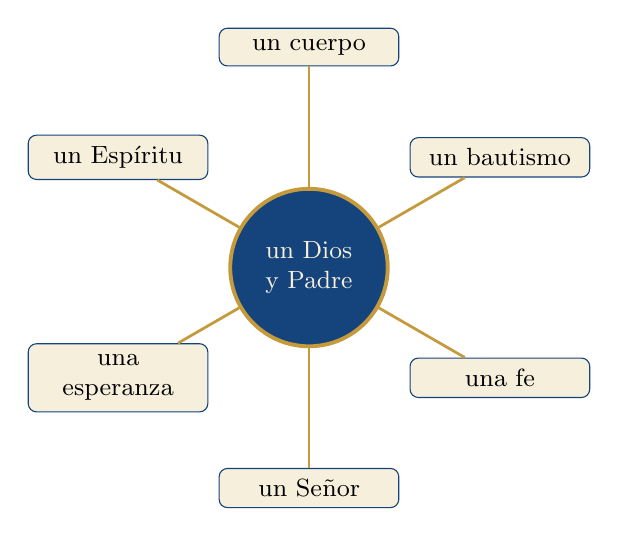
\begin{tikzpicture}[font=\small]
 \node[draw=dorado,line width=1.4pt,fill=azul,text=papiro,circle,minimum size=2.0cm,align=center] (d) at (0,0) {un Dios\\ y Padre};
 \foreach \a/\t in {90/{un cuerpo},150/{un Espíritu},210/{una esperanza},270/{un Señor},330/{una fe},30/{un bautismo}}{
   \node[draw=azul,fill=papiro,rounded corners=3pt,inner sep=4pt,text width=2.0cm,align=center] (n\a) at (\a:2.8) {\t};
   \draw[dorado,line width=1pt] (d)--(n\a);}
\end{tikzpicture}\par
{\footnotesize\color{gris}\textit{Figura 5.} Las siete unidades de Ef 4:4--6. \textit{Nota.} Elaboración propia.}
\end{center}

\subsection{Toda rodilla: Isaías 45 en Filipenses 2}
El texto más fuerte del monoteísmo de Isaías termina con un juramento:

\begin{verso}{Isaías 45:22–23}
Mirad a mí, y sed salvos, todos los términos de la tierra, porque yo soy Dios, y no hay más. Por mí mismo hice juramento, de mi boca salió palabra en justicia, y no será revocada: Que a mí se doblará toda rodilla, y jurará toda lengua.
\end{verso}

Pablo lo aplica a Jesús:

\begin{verso}{Filipenses 2:9–11}
Por lo cual Dios también le exaltó hasta lo sumo, y le dio un nombre que es sobre todo nombre, para que en el nombre de Jesús se doble toda rodilla de los que están en los cielos, y en la tierra, y debajo de la tierra; y toda lengua confiese que Jesucristo es el Señor, para gloria de Dios Padre.
\end{verso}

El ``nombre que es sobre todo nombre'' es el Nombre del Uno, y el ``uno su nombre'' de Zac 14:9 se cumple en la confesión ``Jesucristo es el Señor''. Todo termina ``para gloria de Dios Padre'': la unidad no se rompe. En Ro 14:11 Pablo cita el mismo Is 45:23 a propósito del juicio de Dios.

\precision{la lectura de Flp 2:9--11 a la luz de Is 45:22--23 es de Bauckham (2008). Que el ``nombre sobre todo nombre'' sea el Nombre divino es la interpretación mayoritaria; otros lo entienden como el título ``Señor''. Ambas lecturas convergen.}

\subsection{“Yo y el Padre uno somos”}
La confesión de Pablo hunde sus raíces en las palabras de Jesús. En Jerusalén, durante la fiesta de la Dedicación, los judíos le preguntan si él es el Cristo, y Jesús responde hablando de sus ovejas:

\begin{verso}{Juan 10:28–30}
y yo les doy vida eterna; y no perecerán jamás, ni nadie las arrebatará de mi mano. Mi Padre que me las dio, es mayor que todos, y nadie las puede arrebatar de la mano de mi Padre. Yo y el Padre uno somos.
\end{verso}

\begin{filologia}{Jn 10:30}
\grc{ἐγὼ καὶ ὁ πατὴρ} & --- & ``yo y el Padre'': dos sujetos que se nombran por separado. \\
\grc{ἕν ἐσμεν} & \grc{εἷς} & ``uno somos'': \grc{ἕν} es neutro, ``una sola cosa''; no dice ``una sola persona'' (que sería masculino, \grc{εἷς}), sino una sola realidad de vida, voluntad y obra. \\
\end{filologia}

El argumento de Jesús es el de las dos manos. Nadie arrebata las ovejas de la mano del Hijo (v.~28) y nadie las arrebata de la mano del Padre (v.~29), porque se trata de una sola mano: ``Yo y el Padre uno somos''. La estructura es la misma de Gn 2:24: dos que se nombran por separado y forman una sola unidad. Jesús lo explica en otros pasajes: ``todo lo que el Padre hace, también lo hace el Hijo igualmente'' (Jn 5:19); ``¿No crees que yo soy en el Padre, y el Padre en mí?'' (Jn 14:10). No hay en Dios dos voluntades que negocian, sino una armonía perfecta, y por eso, cuando ora por sus discípulos, Jesús pone esa unidad como modelo:

\begin{verso}{Juan 17:22}
La gloria que me diste, yo les he dado, para que sean uno, así como nosotros somos uno.
\end{verso}

\subsection{“Una sola carne”: el gran misterio}
Pablo toma el texto del matrimonio y lo lleva hasta Cristo:

\begin{verso}{Efesios 5:31–32}
Por esto dejará el hombre a su padre y a su madre, y se unirá a su mujer, y los dos serán una sola carne. Grande es este misterio; mas yo digo esto respecto de Cristo y de la iglesia.
\end{verso}

Pablo cita Gn 2:24 según la Septuaginta, \grc{οἱ δύο εἰς σάρκα μίαν}, y le da su alcance último: la unión de Cristo con su pueblo. En 1~Corintios vuelve al mismo texto con el mismo verbo: ``¿O no sabéis que el que se une con una ramera, es un cuerpo con ella? Porque dice: Los dos serán una sola carne. Pero el que se une al Señor, un espíritu es con él'' (1~Co 6:16--17). ``Se une'', \grc{κολλώμενος}, es el verbo con que la Septuaginta traduce el \heb{דבק} de Gn 2:24, \grc{προσκολληθήσεται}. La adhesión que Deuteronomio pedía al Dios uno (Dt 10:20) se cumple en la unión con Cristo.

\precision{la relación entre \grc{κολλάω} en 1~Co 6:17 y \heb{דבק} en Gn 2:24 y Dt 10:20 se apoya en el vocabulario de la Septuaginta; la conexión con Dt 10:20 es observación propia. La autoría paulina de Efesios se discute; 1~Co 6:16--17 dice lo mismo en una carta indiscutida.}

\subsection{La plenitud del Uno en Cristo}
Los demás escritos del Nuevo Testamento dicen lo mismo con otras palabras. Pablo llama a Cristo el único mediador, ``Porque hay un solo Dios, y un solo mediador entre Dios y los hombres, Jesucristo hombre'' (1~Ti 2:5), y formula la tesis de esta serie: ``en él habita corporalmente toda la plenitud de la Deidad'' (Col 2:9). El Uno no se divide en Cristo; en Cristo se da a conocer.

\begin{center}
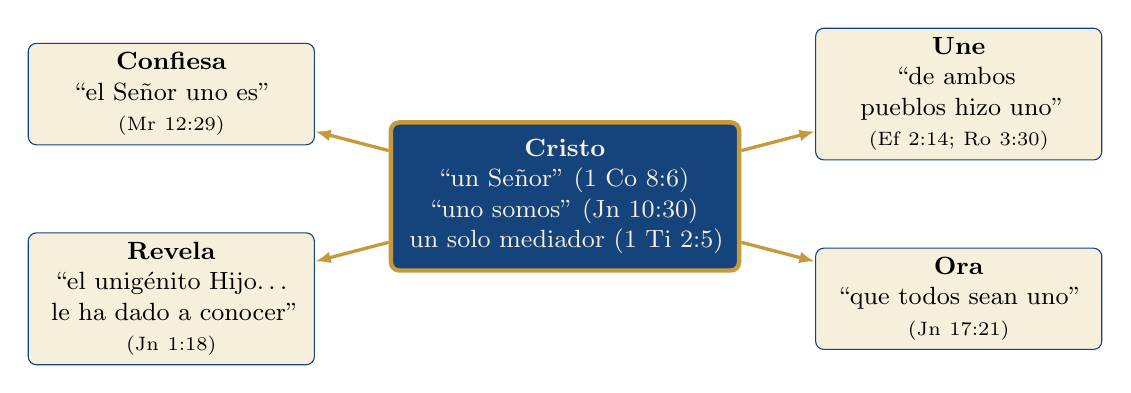
\begin{tikzpicture}[font=\small]
 \node[draw=azul,fill=papiro,rounded corners=3pt,text width=3.4cm,align=center] (a) at (-5.0,1.3) {\textbf{Confiesa}\\ ``el Señor uno es''\\ {\scriptsize(Mr 12:29)}};
 \node[draw=azul,fill=papiro,rounded corners=3pt,text width=3.4cm,align=center] (b) at (-5.0,-1.3) {\textbf{Revela}\\ ``el unigénito Hijo\ldots{} le ha dado a conocer''\\ {\scriptsize(Jn 1:18)}};
 \node[draw=azul,fill=papiro,rounded corners=3pt,text width=3.4cm,align=center] (c) at (5.0,1.3) {\textbf{Une}\\ ``de ambos pueblos hizo uno''\\ {\scriptsize(Ef 2:14; Ro 3:30)}};
 \node[draw=azul,fill=papiro,rounded corners=3pt,text width=3.4cm,align=center] (d) at (5.0,-1.3) {\textbf{Ora}\\ ``que todos sean uno''\\ {\scriptsize(Jn 17:21)}};
 \node[draw=dorado,line width=1.6pt,fill=azul,text=papiro,rounded corners=3pt,text width=4.0cm,align=center,inner sep=6pt] (x) at (0,0) {\textbf{Cristo}\\ ``un Señor'' (1~Co 8:6)\\ ``uno somos'' (Jn 10:30)\\ un solo mediador (1~Ti 2:5)};
 \foreach \n in {a,b,c,d}\draw[dorado,line width=1.2pt,-{Latex[length=2mm]}] (x)--(\n);
\end{tikzpicture}\par
{\footnotesize\color{gris}\textit{Figura 6.} La unidad de Dios en Cristo. \textit{Nota.} Elaboración propia.}
\end{center}

\precision{en Jn 10:30 ``uno'' es neutro (\grc{ἕν}): ``una sola cosa'', no ``una sola persona''. Juan no es de Pablo, y la autoría de 1~Timoteo y Colosenses se discute; la idea paulina central está en 1~Co 8:6, una carta indiscutida.}

%===================================================================
\section{Aplicación: un corazón no dividido}

La unidad de Dios es incomunicable: solo Dios es Dios. Pero el \emph{Shemá} no termina en el v.~4, sino que continúa con ``y amarás'' (v.~5), y lo que el atributo produce en el creyente es un corazón entero.

\begin{enumerate}
\item \textbf{No claudicar entre dos.} El corazón no se reparte entre Dios y otros ``dioses'', sean el dinero, el prestigio o el poder: ``¿Hasta cuándo claudicaréis vosotros entre dos pensamientos?'' (1~R 18:21). Jesús lo dijo con otras palabras: ``Ninguno puede servir a dos señores\ldots{} No podéis servir a Dios y a las riquezas'' (Mt 6:24).
\item \textbf{Pedir un corazón unido.} La petición del salmista, ``unifica mi corazón'' (Sal 86:11), es la oración que corresponde a un Dios uno.
\item \textbf{Oír cada día.} La confesión se convierte en hábito, como manda el propio texto: ``y hablarás de ellas estando en tu casa, y andando por el camino, y al acostarte, y cuando te levantes'' (Dt 6:7).
\item \textbf{Guardar la unidad.} El Dios uno vive en armonía, y su imagen se reconoce donde dos son uno sin dejar de ser dos: en el matrimonio, ``lo que Dios juntó, no lo separe el hombre'' (Mt 19:6), y en la iglesia, que contradice a su Dios cada vez que se divide. La unidad no se fabrica; se guarda (Ef 4:3), porque Cristo oró por ella: ``así como nosotros somos uno'' (Jn 17:22).
\item \textbf{Ser testigos.} Israel fue llamado a ser testigo del Uno ante las naciones (Is 43:10), y quien confiesa que Dios es uno lleva su Nombre a ``todos los términos de la tierra'' (Is 45:22; Ro 3:29).
\end{enumerate}

Santiago advierte contra una confesión sin corazón:

\begin{verso}{Santiago 2:19}
Tú crees que Dios es uno; bien haces. También los demonios creen, y tiemblan.
\end{verso}

Santiago cita el \emph{Shemá}, \grc{εἷς ἐστιν ὁ θεός}, para mostrar que es posible confesar la unidad de Dios con los labios y tener el corazón dividido: la ortodoxia sin amor es la fe de los demonios. La pregunta que deja el atributo alcanza a cada lector: entre qué dos pensamientos claudica hoy.

%===================================================================
\section{Síntesis}

\begin{tcolorbox}[colback=papiro,colframe=azul,boxrule=1pt,arc=3pt]
Dios es uno: no hay otro fuera de él (Dt 4:35), no tiene igual (Is 46:9) ni se divide (Dt 6:4). Israel lo confiesa cada día en el \emph{Shemá} y lo espera para toda la tierra: ``\SENOR{} será uno, y uno su nombre'' (Zac 14:9). En el Carmelo el pueblo deja de claudicar entre dos (1~R 18:39), y los sabios hacen del ``uno'' la aceptación del Reino y la última palabra de los mártires. Su unidad es armonía perfecta: el Dios que dijo ``hagamos'' (Gn 1:26) hizo de dos ``una sola carne'' (Gn 2:24), y en Cristo se oye: ``Yo y el Padre uno somos'' (Jn 10:30). Pablo confiesa el mismo \emph{Shemá} en Cristo, ``un Dios, el Padre\ldots{} y un Señor, Jesucristo'' (1~Co 8:6), y deduce de él un solo pueblo de judíos y gentiles (Ro 3:30).
\end{tcolorbox}

\begin{center}\small\renewcommand{\arraystretch}{1.3}
\begin{tabular}{@{}L{3.0cm}L{11.4cm}@{}}
\toprule
\textbf{Mirada} & \textbf{Aporte al atributo} \\ \midrule
Hebrea & Dt 6:4--9; 4:35, 39; 10:20; Éx 20:3; Zac 14:9; \emph{ejad} (Gn 2:24), \emph{levad}, \emph{ein od}; Is 43--46; Mal 2:10; Sal 86:10--11; Elías en el Carmelo (1~R 18). \\
Judía & Yugo del Reino (Misná \emph{Berajot} 2:2); prolongar el ``uno'' (\emph{Berajot} 13b); Jacob y sus hijos (\emph{Pesajim} 56a); ``no son dos poderes'' (\emph{Mejiltá}); el \emph{Sifré} y Rashi sobre Zac 14:9; Maimónides; Akiva (\emph{Berajot} 61b); \emph{Neilá}; filacterias y Papiro Nash. \\
Teológica & Dios ``está solo en su excelencia'': la unicidad, la autosuficiencia y el conocimiento por revelación; la unidad como armonía: ``hagamos'' (Gn 1:26), ``una sola carne'' (Gn 2:24), ``uno somos'' (Jn 10:30). \\
Paulina & 1~Co 8:4--6; 6:16--17; Ro 3:29--30; 10:12--13; Ef 4:3--6; 2:14--15; 5:31--32; Flp 2:9--11 con Is 45:23; Col 2:9. \\
\bottomrule
\end{tabular}\par
{\footnotesize\color{gris}\textit{Tabla 7.} Síntesis del capítulo. \textit{Nota.} Elaboración propia.}
\end{center}

\begin{verso}{Jeremías 9:24 [9:23]}
Mas alábese en esto el que se hubiere de alabar: en entenderme y conocerme, que yo soy \SENOR{}, que hago misericordia, juicio y justicia en la tierra; porque estas cosas quiero, dice \SENOR{}.
\end{verso}

``Que yo soy \SENOR'': conocer a Dios empieza por saber que no hay otro, y por amarlo con un corazón que tampoco tenga otro.

%===================================================================
\section*{Compendio bíblico}
\begin{center}\small\renewcommand{\arraystretch}{1.12}
\begin{tabular}{@{}L{2.2cm}L{5.0cm}|L{2.2cm}L{5.0cm}@{}}
\toprule
Gn 1:26 & ``Hagamos al hombre'' & Mt 19:6 & ``no son ya más dos'' \\
Gn 2:24 & ``serán una sola carne'' & Jn 5:19 & ``también lo hace el Hijo'' \\
Éx 15:11 & ``¿Quién como tú\ldots?'' & Mr 12:29 & ``el Señor uno es'' \\
Éx 20:3 & ``No tendrás dioses ajenos'' & Mr 12:32 & ``uno es Dios, y no hay otro'' \\
Dt 4:35 & ``no hay otro fuera de él'' & Jn 10:30 & ``Yo y el Padre uno somos'' \\
Dt 4:39 & ``arriba en el cielo y abajo'' & Jn 17:3 & ``el único Dios verdadero'' \\
Dt 6:4--5 & ``\SENOR{} uno es'' & Jn 17:22 & ``así como nosotros somos uno'' \\
Dt 32:39 & ``no hay dioses conmigo'' & Ro 3:29--30 & ``Dios es uno'' \\
1~R 18:21 & ``¿Hasta cuándo claudicaréis?'' & Ro 10:12 & ``el mismo que es Señor de todos'' \\
1~R 18:39 & ``¡\SENOR{} es el Dios!'' & Ro 16:27 & ``al único y sabio Dios'' \\
Neh 9:6 & ``Tú solo eres \SENOR'' & 1~Co 8:4--6 & ``un Dios\ldots{} y un Señor'' \\
Sal 86:10--11 & ``sólo tú eres Dios'' & 1~Co 6:17 & ``un espíritu es con él'' \\
Sal 96:5 & ``los dioses\ldots{} son ídolos'' & Gá 3:20 & ``Dios es uno'' \\
Is 43:10--11 & ``Vosotros sois mis testigos'' & Ef 4:4--6 & ``un Dios y Padre de todos'' \\
Dt 10:20 & ``a él seguirás'' & Ef 5:31--32 & ``Grande es este misterio'' \\
Is 44:6 & ``fuera de mí no hay Dios'' & Flp 2:10--11 & ``se doble toda rodilla'' \\
Is 45:5--6 & ``no hay más que yo'' & Col 2:9 & ``toda la plenitud de la Deidad'' \\
Is 45:22--23 & ``a mí se doblará toda rodilla'' & 1~Ti 1:17 & ``al único y sabio Dios'' \\
Is 46:9 & ``nada hay semejante a mí'' & 1~Ti 2:5 & ``un solo Dios, y un solo mediador'' \\
Jer 32:39 & ``un corazón, y un camino'' & 1~Ti 6:15--16 & ``el bienaventurado y solo Soberano'' \\
Zac 14:9 & ``uno su nombre'' & Stg 2:19 & ``Tú crees que Dios es uno'' \\
\bottomrule
\end{tabular}\par
{\footnotesize\color{gris}\textit{Tabla 8.} Compendio bíblico de la unidad de Dios. \textit{Nota.} Textos de la RVR1960.}
\end{center}

%===================================================================
\section*{Glosario del capítulo}
\begin{description}\setlength{\itemsep}{2pt}
\item[\emph{Alenu}] Oración que cierra los servicios de la sinagoga; termina con Zac 14:9.
\item[\emph{Ani hu}] (\heb{אֲנִי הוּא}). ``Yo (soy) él'' (Dt 32:39; Is 43:10); en la LXX, \grc{ἐγώ εἰμι}.
\item[\emph{Dabaq}] (\heb{דָּבַק}). Adherirse, unirse: al cónyuge (Gn 2:24) y a Dios (Dt 10:20).
\item[\emph{Ed}] (\heb{עֵד}). Testigo; lo forman las letras grandes de Dt 6:4.
\item[\emph{Ein od}] (\heb{אֵין עוֹד}). ``No hay otro'' (Dt 4:35; Is 45:5).
\item[\emph{Ejad}] (\heb{אֶחָד}). Uno, uno solo, el mismo (Dt 6:4; Zac 14:9).
\item[\emph{Heîs}] (\grc{εἷς}). Uno (Mr 12:29; 1~Co 8:6).
\item[\emph{Levad}] (\heb{לְבַד}). Solo, aparte (Neh 9:6; Sal 86:10).
\item[\emph{Mónos}] (\grc{μόνος}). Solo, único (Jn 17:3; Ro 16:27).
\item[\emph{Na'asé}] (\heb{נַעֲשֶׂה}). ``Hagamos'' (Gn 1:26).
\item[\emph{Neilá}] Oración final del Día de la Expiación.
\item[\emph{Ol maljut shamáyim}] ``Yugo del Reino de los cielos'' (Misná \emph{Berajot} 2:2).
\item[\emph{Pasaj}] (\heb{פסח}). Cojear, saltar: ``claudicar'' (1~R 18:21).
\item[\emph{Shemá}] (\heb{שְׁמַע}). ``Oye''; nombre de Dt 6:4--9 y de la oración diaria.
\item[Simplicidad] Término teológico: Dios no está compuesto de partes.
\item[\emph{Tefilín}] Filacterias: cajas pequeñas con Dt 6:4--9 y otros textos (Dt 6:8).
\item[\emph{Yajed}] (\heb{יַחֵד}). Unificar (Sal 86:11).
\item[\emph{Yajid}] (\heb{יָחִיד}). Único, hijo único (Gn 22:2).
\end{description}


% \chapter{...}% Capítulo: Dios es amor (generado desde ../02_Amor/02_Amor_capitulo.tex)
% Texto ancla: 1 Juan 4:7–16. Clasificación: Ser; incomunicable en su plenitud, comunicable como reflejo.

\section{Un atributo del ser}

Pocas palabras se usan tanto y se entienden tan poco como ``amor''. En el lenguaje de hoy suele significar un sentimiento intenso, espontáneo y cambiante; y, aplicado a Dios, una indulgencia que lo tolera todo. Pink advertía que muchos hablan del amor de Dios sin conocer al Dios de amor, y que la idea común lo reduce a una emoción blanda modelada según la nuestra (Pink, 2020, cap.~16). La Escritura no corrige ese error con una definición abstracta, sino con tres afirmaciones sobre lo que Dios \emph{es}:

\begin{center}\small\renewcommand{\arraystretch}{1.2}
\begin{tabular}{@{}L{3.6cm}L{3.0cm}L{8.2cm}@{}}
\toprule
\textbf{Afirmación} & \textbf{Texto} & \textbf{Lo que dice de Dios} \\ \midrule
``Dios es Espíritu'' & Jn 4:24 & Su modo de ser: no está limitado a un lugar ni a un cuerpo. \\
``Dios es luz'' & 1 Jn 1:5 & Su pureza: ``no hay ningunas tinieblas en él''. \\
``Dios es amor'' & 1 Jn 4:8, 16 & Su vida misma: el amor no es algo que Dios tenga, sino lo que es. \\
\bottomrule
\end{tabular}\par
{\footnotesize\color{gris}\textit{Tabla 1.} Las tres afirmaciones ``Dios es''. \textit{Nota.} Elaboración propia a partir de Pink (2020, cap.~16).}
\end{center}

Por eso esta serie pone el amor entre los atributos del \destacar{Ser}, junto a la unidad y la espiritualidad. Decir que Dios ama describe lo que hace; decir que Dios \emph{es} amor describe lo que es antes de hacer cualquier cosa, antes de que existiera una criatura a quien amar. Pink lo dice así: ``No es simplemente que Dios `ama', sino que Él es el amor mismo. El amor no es meramente uno de sus atributos, sino su propia naturaleza'' (Pink, 2020, p.~83).

\precision{clasificación propuesta: atributo del Ser. Es \emph{incomunicable} en su plenitud (solo el amor de Dios es eterno, sin causa fuera de sí e invariable) y \emph{comunicable} como reflejo: ``Amados, si Dios nos ha amado así, debemos también nosotros amarnos unos a otros'' (1 Jn 4:11). Queda sujeta a la revisión del autor de la serie.}

El autor de esta serie resumió el atributo en tres palabras: el amor de Dios es \destacar{eterno}, \destacar{soberano} e \destacar{inmutable}. Las tres responden a la misma pregunta desde ángulos distintos. ¿Cuándo empezó? Nunca: es eterno. ¿Qué lo causó? Nada fuera de Dios: es soberano. ¿Puede acabar? No: es inmutable. Los tres rasgos se siguen aquí desde los textos hebreos y desde Pablo; de ellos se desprende que ese amor es también santo, y que en Cristo se revela infinito y lleno de gracia (Ef 3:19; Ro 8:32).

\begin{center}\small\renewcommand{\arraystretch}{1.2}
\begin{tabular}{@{}L{2.4cm}L{4.6cm}L{4.0cm}L{3.8cm}@{}}
\toprule
\textbf{Rasgo} & \textbf{Pregunta} & \textbf{Texto hebreo} & \textbf{Texto paulino} \\ \midrule
Eterno & ¿Cuándo empezó? & ``Con amor eterno te he amado'' (Jer 31:3) & ``antes de la fundación del mundo'' (Ef 1:4--5) \\
Soberano & ¿Qué lo causó? & ``No por ser vosotros más\ldots{} sino por cuanto el \SENOR{} os amó'' (Dt 7:7--8) & ``según el puro afecto de su voluntad'' (Ef 1:5); ``A Jacob amé'' (Ro 9:13) \\
Inmutable & ¿Puede acabar? & ``Yo \SENOR{} no cambio'' (Mal 3:6); ``¿Cómo podré abandonarte?'' (Os 11:8) & ``nada nos podrá separar'' (Ro 8:38--39) \\
\bottomrule
\end{tabular}\par
{\footnotesize\color{gris}\textit{Tabla 2.} El eje del capítulo. \textit{Nota.} Elaboración propia.}
\end{center}

%===================================================================
\section{Texto ancla: 1 Juan 4:7--16}

\subsection{El contexto}
Juan escribe a iglesias sacudidas por maestros que se habían ido de la comunidad y negaban que Jesús fuera el Cristo venido en carne (1 Jn 2:18--19, 22; 4:1--3). Contra ellos, la carta da tres pruebas de la vida verdadera: creer que Jesús es el Hijo de Dios, obedecer sus mandamientos y amar a los hermanos. En el capítulo 4, la tercera prueba se apoya en la teología más alta de la carta: el amor entre hermanos no es una virtud social; viene de lo que Dios es.

\precision{1 Juan no es una carta de Pablo. Se usa como texto ancla porque contiene la afirmación ``Dios es amor'' y porque así lo pidió el autor de la serie. La lectura paulina del atributo se desarrolla en la sección~\ref{sec:cristo-amor}.}

\subsection{El texto}
\begin{verso}{1 Juan 4:7–10}
Amados, amémonos unos a otros; porque el amor es de Dios. Todo aquel que ama, es nacido de Dios, y conoce a Dios. El que no ama, no ha conocido a Dios; porque Dios es amor. En esto se mostró el amor de Dios para con nosotros, en que Dios envió a su Hijo unigénito al mundo, para que vivamos por él. En esto consiste el amor: no en que nosotros hayamos amado a Dios, sino en que él nos amó a nosotros, y envió a su Hijo en propiciación por nuestros pecados.
\end{verso}

\begin{verso}{1 Juan 4:11–16}
Amados, si Dios nos ha amado así, debemos también nosotros amarnos unos a otros. Nadie ha visto jamás a Dios. Si nos amamos unos a otros, Dios permanece en nosotros, y su amor se ha perfeccionado en nosotros. En esto conocemos que permanecemos en él, y él en nosotros, en que nos ha dado de su Espíritu. Y nosotros hemos visto y testificamos que el Padre ha enviado al Hijo, el Salvador del mundo. Todo aquel que confiese que Jesús es el Hijo de Dios, Dios permanece en él, y él en Dios. Y nosotros hemos conocido y creído el amor que Dios tiene para con nosotros. Dios es amor; y el que permanece en amor, permanece en Dios, y Dios en él.
\end{verso}

\begin{filologia}{1 Jn 4:8--10}
\grc{ὁ θεὸς ἀγάπη ἐστίν} & \grc{ἀγάπη} & ``Dios es amor'': \emph{ho theós} lleva artículo y es el sujeto; \emph{agápē} no lo lleva y es el predicado. La frase no es reversible: no dice ``el amor es Dios'', sino que el amor describe lo que Dios es. \\
\grc{ἐν τούτῳ ἐφανερώθη} & \grc{φανερόω} & ``En esto se mostró'': se hizo visible en la historia. El amor que Dios es se manifiesta en un acto: el envío del Hijo. \\
\grc{τὸν μονογενῆ} \emph{monogenē} & \grc{μόνος} & ``unigénito'', único en su clase: el Hijo amado y único (cf. Gn 22:2). \\
\grc{ἠγάπησεν ἡμᾶς} & \grc{ἀγαπάω} & ``él nos amó'': aoristo, un acto concreto. Contrasta con el perfecto \grc{ἠγαπήκαμεν}, ``nosotros hayamos amado''. \\
\grc{ἱλασμόν} \emph{hilasmós} & \grc{ἱλάσκομαι} & ``propiciación'': el sacrificio que aparta la ira (véase el capítulo sobre la ira santa). El amor de Dios no ignora el pecado: lo cubre a su propio costo. \\
\end{filologia}

\subsection{Cuatro veces “en esto”}
El pasaje se ordena con la fórmula \grc{ἐν τούτῳ}, ``en esto'' (4:9, 10, 13, 17). Cada vez responde a una pregunta distinta sobre el amor:

\begin{center}\small\renewcommand{\arraystretch}{1.2}
\begin{tabular}{@{}L{1.6cm}L{4.4cm}L{8.8cm}@{}}
\toprule
\textbf{Verso} & \textbf{``En esto\ldots''} & \textbf{Respuesta} \\ \midrule
4:9 & se \emph{mostró} el amor & Dios envió a su Hijo unigénito para que vivamos por él. \\
4:10 & \emph{consiste} el amor & No en nuestro amor a Dios, sino en que él nos amó primero y envió a su Hijo en propiciación. \\
4:13 & \emph{conocemos} que permanecemos & Nos ha dado de su Espíritu. \\
4:17 & se ha \emph{perfeccionado} el amor & Tenemos confianza en el día del juicio. \\
\bottomrule
\end{tabular}\par
{\footnotesize\color{gris}\textit{Tabla 3.} La estructura de 1 Jn 4:9--17. \textit{Nota.} Elaboración propia.}
\end{center}

El orden es teológico. Primero, lo que Dios es (``Dios es amor''); luego, cómo lo mostró (el envío); después, en qué consiste (la propiciación); finalmente, cómo llega a nosotros (el Espíritu) y adónde nos lleva (confianza ante el juicio). El Padre envía y el Hijo es enviado como propiciación: el amor que Dios es se revela en el Padre que da a su Hijo (Jn 3:16).

\begin{verso}{1 Juan 4:19}
Nosotros le amamos a él, porque él nos amó primero.
\end{verso}

El versículo 19 resume la carta: el amor de Dios va primero. No es respuesta a nuestro amor ni recompensa de él; es su causa. Ese ``primero'' (\grc{πρῶτος}) es la puerta a los tres rasgos de este capítulo: un amor que precede (eterno), que no tiene causa en nosotros (soberano) y que, por lo mismo, no depende de nosotros para seguir (inmutable).

%===================================================================
\section{La palabra: el amor en hebreo y en griego}

\subsection{La raíz \emph{ahav}}
El verbo hebreo principal es \heb{אָהַב} \emph{ahav}, ``amar'', con el sustantivo \heb{אַהֲבָה} \emph{ahavá}, ``amor''. Vine (1999) calcula unas 250 apariciones del verbo; el conteo propio en la BHS da 248 formas de la raíz en 227 versículos. La palabra cubre todo el arco del amor humano: el del esposo por la esposa (Gn 24:67; 29:20), el del padre por el hijo (Gn 22:2; 37:3), el del amigo (1 S 18:1), el del siervo por su señor (Éx 21:5) y la lealtad política (1 R 5:1 [5:15]). Puede designar también el apego a cosas (Pr 21:17) y aun la pasión que destruye (2 S 13:15).

\begin{verso}{Génesis 29:20}
Así sirvió Jacob por Raquel siete años; y le parecieron como pocos días, porque la amaba.
\end{verso}

\begin{verso}{1 Samuel 18:1}
Aconteció que cuando él hubo acabado de hablar con Saúl, el alma de Jonatán quedó ligada con la de David, y lo amó Jonatán como a sí mismo.
\end{verso}

\begin{filologia}{Gn 29:20; 1 S 18:1}
\heb{בְּאַהֲבָתוֹ אֹתָהּ} \emph{be'ahavató otah} & \heb{אהב} & ``porque la amaba'', literalmente ``en su amarla'': el amor acorta el tiempo del servicio. \\
\heb{נִקְשְׁרָה} \emph{niqsherá} & \heb{קשר} & ``quedó ligada'': atada como con un nudo. El amor de amistad une dos vidas. \\
\heb{כְּנַפְשׁוֹ} \emph{kenafshó} & \heb{נפשׁ} & ``como a sí mismo'', ``como a su propia vida''. \\
\end{filologia}

La raíz no tiene, en sí misma, un sentido ``espiritual'' reservado: es la palabra común del amor humano. Por eso sorprende tanto que Dios la use de sí mismo. Cuando lo hace, toma la palabra de la casa, del matrimonio y de la amistad para hablar de su relación con un pueblo.

\subsection{La primera vez: el hijo amado}
La primera aparición del verbo en la Biblia está en el monte Moriah:

\hebverso{קַח־נָא אֶת־בִּנְךָ אֶת־יְחִידְךָ אֲשֶׁר־אָהַבְתָּ אֶת־יִצְחָק}
\begin{verso}{Génesis 22:2}
Y dijo: Toma ahora tu hijo, tu único, Isaac, a quien amas, y vete a tierra de Moriah, y ofrécelo allí en holocausto sobre uno de los montes que yo te diré.
\end{verso}

\begin{filologia}{Gn 22:2}
\heb{יְחִידְךָ} \emph{yejidjá} & \heb{יחד} & ``tu único'': el hijo de la promesa, sin reemplazo. \\
\heb{אֲשֶׁר־אָהַבְתָּ} \emph{asher ahavta} & \heb{אהב} & ``a quien amas'': primera vez que aparece ``amar'' en la Biblia. \\
LXX \grc{τὸν ἀγαπητόν, ὃν ἠγάπησας} & \grc{ἀγαπάω} & La Septuaginta traduce \emph{yajid} por \grc{ἀγαπητός}, ``el amado'', y conserva el verbo: ``al amado, al que amaste''. \\
\end{filologia}

La Biblia empieza a hablar de amor con un padre que ama a su único hijo y un Dios que le pide entregarlo. El Nuevo Testamento retoma ese lenguaje: en el bautismo, el Padre dice ``Este es mi Hijo amado'' (\grc{ὁ υἱός μου ὁ ἀγαπητός}, Mt 3:17), y Pablo escribe que Dios ``no escatimó ni a su propio Hijo'' (Ro 8:32), con el mismo verbo que la Septuaginta usa para Abraham: \grc{οὐκ ἐφείσω τοῦ υἱοῦ σου τοῦ ἀγαπητοῦ}, ``no escatimaste a tu hijo, el amado'' (Gn 22:16 LXX).

\precision{la conexión entre Gn 22 y Ro 8:32 es un eco verbal (\grc{φείδομαι}, ``escatimar''), reconocido por varios comentaristas (Moo, 1996; Dunn, 1998). Es una lectura tipológica: Pablo no cita Génesis, pero su vocabulario remite a la escena de Moriah.}

\subsection{El amor del pacto}
En Deuteronomio, \emph{ahav} se vuelve palabra de pacto. Dios ama a los padres y elige a su descendencia (Dt 4:37; 7:8; 10:15); Israel debe amar a Dios con todo su ser (Dt 6:5; 10:12; 11:1, 13; 30:6, 16, 20). El amor se manda, se guarda y se demuestra en la obediencia: Dios ``guarda el pacto y la misericordia a los que le aman y guardan sus mandamientos'' (Dt 7:9; cf. Éx 20:6).

\hebverso{שְׁמַע יִשְׂרָאֵל יְהוָה אֱלֹהֵינוּ יְהוָה אֶחָד \\ וְאָהַבְתָּ אֵת יְהוָה אֱלֹהֶיךָ בְּכָל־לְבָבְךָ וּבְכָל־נַפְשְׁךָ וּבְכָל־מְאֹדֶךָ}
\begin{verso}{Deuteronomio 6:4–5}
Oye, Israel: \SENOR{} nuestro Dios, \SENOR{} uno es. Y amarás a \SENOR{} tu Dios de todo tu corazón, y de toda tu alma, y con todas tus fuerzas.
\end{verso}

\begin{filologia}{Dt 6:5}
\heb{וְאָהַבְתָּ} \emph{ve'ahavta} & \heb{אהב} & ``y amarás'': perfecto con \emph{vav}, mandato. El amor se puede mandar porque no es solo emoción: es lealtad del corazón. \\
\heb{לְבָבְךָ} \emph{levavjá} & \heb{לבב} & ``tu corazón'': en hebreo, el centro de la voluntad y el pensamiento, no solo del sentimiento. \\
\heb{נַפְשְׁךָ} \emph{nafshejá} & \heb{נפשׁ} & ``tu alma'': la vida misma. \\
\heb{מְאֹדֶךָ} \emph{me'odéja} & \heb{מאד} & ``tus fuerzas'': literalmente ``tu mucho'', todo lo que uno tiene y puede. \\
LXX \grc{ἀγαπήσεις} & \grc{ἀγαπάω} & ``amarás''; Jesús cita el texto como ``el primer mandamiento de todos'' (Mr 12:29--30). \\
\end{filologia}

\precision{el lenguaje de ``amar'' y ``guardar los mandamientos'' tiene paralelos en los tratados del antiguo Oriente, donde el vasallo debía ``amar'' a su soberano, es decir, serle leal. Moran (1963) mostró ese trasfondo para Deuteronomio. El paralelo ilumina el carácter de pacto del amor, pero no lo reduce a un contrato: Deuteronomio funda el amor de Israel en el amor previo y gratuito de Dios (Dt 7:7--8; 10:15).}

\subsection{Las demás palabras del amor}
La Reina-Valera 1960 traduce con ``amor, amores, amar, amado, amante'' varias palabras distintas. El espectro completo, sin contar ``amo'' y ``ama'' cuando significan señor o nodriza, da \textbf{713 apariciones en 608 versículos}: 346 en el Antiguo Testamento (309 versículos) y 367 en el Nuevo (299 versículos). ``Amor'' y ``amores'' suman 238; las formas de ``amado'', 160; las demás formas del verbo, 315.

\begin{center}\small\renewcommand{\arraystretch}{1.18}
\begin{tabular}{@{}L{4.0cm}L{1.5cm}L{4.4cm}L{5.0cm}@{}}
\toprule
\textbf{Término} & \textbf{Raíz} & \textbf{Sentido base} & \textbf{Textos y frecuencia} \\ \midrule
\heb{אָהַב} \emph{ahav}, \heb{אַהֲבָה} \emph{ahavá} & \heb{אהב} & amar, amor (toda clase) & ≈~250; en 195 de los versículos con ``amor/amar'' de la RVR1960 \\
\heb{דּוֹד} \emph{dod} & \heb{דוד} & amado; amores; tío & sobre todo Cantares (≈~35); Is 5:1; Ez 16:8 \\
\heb{יָדִיד} \emph{yedid} & \heb{ידד} & amado, querido & Dt 33:12; Sal 127:2; Is 5:1; Jer 11:15 \\
\heb{חָשַׁק} \emph{jashaq} & \heb{חשׁק} & ligarse, apegarse por amor & Dt 7:7; 10:15 (``os ha querido'', ``se agradó''); Sal 91:14 \\
\heb{רָחַם} \emph{rajam} & \heb{רחם} & amar entrañablemente & Sal 18:1 [18:2]: ``Te amo, oh \SENOR''; en arameo es el verbo común de ``amar'' \\
\heb{חָפֵץ} \emph{jafets}, \heb{רָצָה} \emph{ratsá} & --- & deleitarse, complacerse & Sal 51:6 [51:8]; 1 S 18:22 \\
\heb{לְמַעַן} \emph{lemá'an}, \heb{בַּעֲבוּר} & --- & ``a causa de'', ``por'' & la locución ``por amor de'' (73 veces), que no es vocabulario de amor \\ \midrule
\grc{ἀγαπάω} \emph{agapáō} & \grc{ἀγαπ-} & amar & 143 (NA27) \\
\grc{ἀγάπη} \emph{agápē} & \grc{ἀγαπ-} & amor & 116 \\
\grc{ἀγαπητός} \emph{agapētós} & \grc{ἀγαπ-} & amado & 61 \\
\grc{φιλέω} \emph{philéō}, \grc{φίλος} & \grc{φιλ-} & querer, tener afecto; amigo & 25 y 29 \\
\grc{φιλαδελφία}, \grc{φιλόστοργος}, \grc{φιλανθρωπία} & \grc{φιλ-} & amor fraternal, afecto familiar, amor a los hombres & Ro 12:10; 1 Ts 4:9; Tit 3:4 \\
\grc{σπλάγχνα} \emph{splánjna} & --- & entrañas, afecto & ``entrañable amor'' (Flp 1:8) \\
\bottomrule
\end{tabular}\par
{\footnotesize\color{gris}\textit{Tabla 4.} El espectro del amor en la RVR1960. \textit{Nota.} Conteo propio con la RVR1960 (sin títulos de sección), la BHS y NA27 con números Strong. Las cifras de \emph{dod} son aproximadas porque la misma grafía \heb{דוד} es también el nombre de David.}
\end{center}

\precision{en 73 lugares la RVR1960 dice ``por amor de'' (Sal 23:3; Is 43:25; 48:11; Ro 9:3; Flp 3:7). Casi siempre traduce una preposición causal (\heb{לְמַעַן}, \grc{διά}, \grc{ἕνεκεν}), ``a causa de, por'', y no una palabra de amor. No conviene apoyar en esos textos una doctrina del amor de Dios. El conteo propio debe verificarse en e-Sword.}

Dos palabras merecen nota. La primera es \heb{חָשַׁק} \emph{jashaq} (Dt 7:7; 10:15). Su sentido concreto es ``ligar, sujetar'' (las molduras que ``ciñen'' las columnas del tabernáculo se forman con esta raíz, Éx 27:17; 38:17); usada de afecto, significa poner el corazón sobre alguien y quedar ligado a él (Gn 34:8). La segunda es el arameo: el Targum Ónkelos traduce el ``amarás'' del Shemá con \heb{וְתִרְחַם}, de la raíz \emph{rjm}. En arameo, esa raíz es el verbo común de ``amar''; en hebreo, la misma raíz da \emph{rajamím}, las entrañas de misericordia. El amor y la misericordia de Dios comparten raíz (véase el capítulo sobre la misericordia).

\subsection{El griego: \emph{agapē} y \emph{phileō}}
La Septuaginta tradujo \emph{ahav} casi siempre con \grc{ἀγαπάω}: en el conteo propio, 172 de los 227 versículos con la raíz hebrea llevan esa familia y 23 llevan \grc{φιλέω}. El sustantivo \grc{ἀγάπη} era poco común antes de la Septuaginta, que lo usa sobre todo en Cantares (Cnt 2:4, 5, 7; 8:6, 7); el Nuevo Testamento lo convierte en la palabra central del amor de Dios. \grc{ἔρως}, el deseo, apenas aparece en la Septuaginta (Pr 7:18) y nunca en el Nuevo Testamento.

\precision{es frecuente oír que \emph{agapē} significa por sí misma un amor divino o superior y \emph{phileō} un amor humano o inferior. Carson (2013) llama a esto la ``falacia de la raíz''. Los datos no lo sostienen: en 2 S 13:15 (LXX) \grc{ἀγαπάω} y \grc{ἀγάπη} describen la pasión de Amnón por Tamar; Demas abandona a Pablo ``amando'' (\grc{ἀγαπήσας}) este mundo (2 Ti 4:10); el Padre ama al Hijo con \grc{ἀγαπάω} en Jn 3:35 y con \grc{φιλέω} en Jn 5:20, sin diferencia de sentido. Lo que da contenido a \emph{agapē} en el Nuevo Testamento no es la palabra, sino el acto que la define: ``En esto consiste el amor\ldots{} envió a su Hijo'' (1 Jn 4:10).}

\begin{center}
\begin{tikzpicture}[font=\small, node distance=0.6cm]
 \tikzset{b/.style={draw=azul,line width=0.8pt,fill=papiro,rounded corners=3pt,text width=3.4cm,align=center,inner sep=5pt}}
 \node[b] (h) {\textbf{Hebreo}\\ \heb{וְאַהֲבַת עוֹלָם אֲהַבְתִּיךְ}\\ {\footnotesize Jer 31:3}};
 \node[b,right=of h] (l) {\textbf{LXX}\\ \grc{ἀγάπησιν αἰωνίαν ἠγάπησά σε}\\ {\footnotesize Jer 38:3}};
 \node[b,right=of l] (p) {\textbf{Pablo}\\ \grc{ὁ ἀγαπήσας ἡμᾶς καὶ δοὺς παράκλησιν αἰωνίαν}\\ {\footnotesize 2 Ts 2:16}};
 \draw[-{Latex[length=3mm]},dorado,line width=1.4pt] (h)--(l);
 \draw[-{Latex[length=3mm]},dorado,line width=1.4pt] (l)--(p);
\end{tikzpicture}\par
{\footnotesize\color{gris}\textit{Figura 1.} De \emph{ahavá} a \emph{agapē}: el amor eterno pasa del profeta al apóstol. \textit{Nota.} Elaboración propia (BHS, Rahlfs-Hanhart, NA28).}
\end{center}

%===================================================================
\section{El Nombre que revela el amor}\label{sec:nombre-amor}

La Escritura hebrea no tiene un nombre propio de Dios formado con \emph{ahav}. El amor se revela, más bien, en los nombres que Dios \emph{da}: llama ``amado'' a quien ama. El Nuevo Testamento, en cambio, sí pone el amor en el nombre mismo de Dios y en los títulos del Hijo.

\precision{la tradición judía enseña que Dios es llamado según sus obras: Elohim cuando juzga, \emph{Tsevaot} cuando hace guerra contra los impíos, \emph{El Shadday} cuando suspende el castigo y el Nombre de cuatro letras cuando tiene misericordia (\emph{Shemot Rabá} 3:6). Esta sección aplica ese principio al amor: no hay un ``nombre de amor'' en la Torá, pero sí nombres que Dios da por amor.}

\subsection{“Jedidías”: amado del \SENOR}
Después del pecado de David con Betsabé y de la muerte del primer hijo, nace Salomón. El texto añade algo que no dice de ningún otro rey:

\hebverso{וַיִּקְרָא אֶת־שְׁמוֹ שְׁלֹמֹה וַיהוָה אֲהֵבוֹ \\ וַיִּשְׁלַח בְּיַד נָתָן הַנָּבִיא וַיִּקְרָא אֶת־שְׁמוֹ יְדִידְיָהּ בַּעֲבוּר יְהוָה}
\begin{verso}{2 Samuel 12:24–25}
Y consoló David a Betsabé su mujer, y llegándose a ella durmió con ella; y ella le dio a luz un hijo, y llamó su nombre Salomón, al cual amó \SENOR, y envió un mensaje por medio de Natán profeta; así llamó su nombre Jedidías, a causa de \SENOR.
\end{verso}

\begin{filologia}{2 S 12:24--25}
\heb{וַיהוָה אֲהֵבוֹ} \emph{vaAdonay ahevó} & \heb{אהב} & ``y el \SENOR{} lo amó'': el sujeto va primero, para destacar quién ama. \\
\heb{יְדִידְיָהּ} \emph{Yedidyah} & \heb{ידד} & ``amado de \emph{Yah}'': \emph{yedid}, ``amado, querido'', más la forma breve del Nombre. Es el único lugar donde aparece. \\
\heb{בַּעֲבוּר יְהוָה} \emph{ba'avur Adonay} & --- & ``a causa del \SENOR'': el nombre no se debe a David ni al niño, sino a Dios. \\
\end{filologia}

El nombre llega por medio de Natán, el mismo profeta que había denunciado el pecado de David (2 S 12:7). El amor de Dios se nombra justo donde menos se esperaba: en el hijo de una unión que había empezado con adulterio y homicidio. Es el amor soberano de Dt 7:7--8 hecho nombre propio.

\precision{ver en ``Jedidías'' una revelación del amor soberano y de la gracia después del pecado es una lectura propia de esta serie, apoyada en el contexto inmediato (2 S 12:13--25).}

\subsection{“El Dios de amor y de paz”}
El único lugar de la Biblia donde el amor forma parte del nombre de Dios está al final de 2 Corintios, la carta más dolorosa de Pablo:

\begin{verso}{2 Corintios 13:11}
Por lo demás, hermanos, tened gozo, perfeccionaos, consolaos, sed de un mismo sentir, y vivid en paz; y el Dios de paz y de amor estará con vosotros.
\end{verso}

\begin{filologia}{2 Co 13:11}
\grc{ὁ θεὸς τῆς ἀγάπης καὶ εἰρήνης} & \grc{ἀγάπη} & ``el Dios del amor y de la paz''. El griego pone primero el amor; la RVR1960 invierte el orden. La expresión ``Dios del amor'' no aparece en ningún otro lugar del Nuevo Testamento (conteo propio en NA27). \\
\grc{εἰρήνη} & \heb{שָׁלוֹם} & ``paz'': en Pablo, eco del \emph{shalom} hebreo, la plenitud de la relación restaurada. \\
\grc{ἔσται μεθ᾽ ὑμῶν} & \grc{εἰμί} & ``estará con vosotros'': promesa de presencia, como \heb{אֶהְיֶה עִמָּךְ}, ``yo estaré contigo'' (Éx 3:12). \\
\end{filologia}

Tres versículos después, la carta termina con la bendición más completa de Pablo: ``La gracia del Señor Jesucristo, el amor de Dios, y la comunión del Espíritu Santo sean con todos vosotros'' (2 Co 13:14). El amor se atribuye a Dios Padre, entre la gracia del Hijo y la comunión del Espíritu.

\subsection{“El Amado” y “el Hijo de su amor”}
Pablo también nombra al Hijo por el amor del Padre. Dios ``nos hizo aceptos en el Amado'' (\grc{ἐν τῷ ἠγαπημένῳ}, Ef 1:6), y ``nos ha trasladado al reino de su amado Hijo'', literalmente ``del Hijo de su amor'' (\grc{τοῦ υἱοῦ τῆς ἀγάπης αὐτοῦ}, Col 1:13). Los dos títulos remiten a la voz del bautismo, ``Este es mi Hijo amado'' (Mt 3:17), y detrás de ella a Moriah: ``tu hijo, tu único, a quien amas'' (Gn 22:2).

\subsection{La liturgia: “el que ama a su pueblo Israel”}
La oración judía cierra las dos bendiciones sobre el amor de Dios con un título. La de la tarde, \emph{Ahavat olam}, termina: \heb{בָּרוּךְ אַתָּה יְהוָה אוֹהֵב עַמּוֹ יִשְׂרָאֵל}, ``Bendito eres tú, \SENOR, que amas a tu pueblo Israel''. La de la mañana, \emph{Ahavá rabbá}, termina: \heb{הַבּוֹחֵר בְּעַמּוֹ יִשְׂרָאֵל בְּאַהֲבָה}, ``que escoges a tu pueblo Israel con amor''. Son participios usados como títulos: Dios es nombrado ``el que ama'' y ``el que elige en amor''.

\precision{las fórmulas son litúrgicas (sidur asquenazí, oraciones de la tarde y de la mañana), no bíblicas. Se citan como testimonio de cómo Israel nombra a Dios por su amor; la segunda une, como Deuteronomio 7, amor y elección.}

\begin{center}\small\renewcommand{\arraystretch}{1.2}
\begin{tabular}{@{}L{3.6cm}L{4.0cm}L{2.4cm}L{4.8cm}@{}}
\toprule
\textbf{Nombre o título} & \textbf{Hebreo / griego} & \textbf{Texto} & \textbf{Qué revela} \\ \midrule
Jedidías, ``amado del \SENOR'' & \heb{יְדִידְיָהּ} & 2 S 12:25 & El amor soberano que se nombra después del pecado. \\
``Dios es amor'' & \grc{ὁ θεὸς ἀγάπη ἐστίν} & 1 Jn 4:8, 16 & El amor como lo que Dios es. \\
El Dios del amor y de la paz & \grc{ὁ θεὸς τῆς ἀγάπης καὶ εἰρήνης} & 2 Co 13:11 & El amor en el nombre de Dios, con promesa de presencia. \\
El Amado & \grc{ὁ ἠγαπημένος} & Ef 1:6 & El Hijo amado, en quien somos aceptados. \\
El Hijo de su amor & \grc{ὁ υἱὸς τῆς ἀγάπης αὐτοῦ} & Col 1:13 & El amor eterno del Padre por el Hijo. \\
``El que ama a su pueblo Israel'' & \heb{אוֹהֵב עַמּוֹ יִשְׂרָאֵל} & Liturgia (\emph{Ahavat olam}) & El amor de pacto, confesado en la oración. \\
\bottomrule
\end{tabular}\par
{\footnotesize\color{gris}\textit{Tabla 5.} Nombres y títulos que revelan el amor de Dios. \textit{Nota.} Elaboración propia (BHS, NA28, sidur asquenazí).}
\end{center}

%===================================================================
\section{Definición}

\subsection{¿Qué es el amor de Dios?}
Reuniendo los textos, se propone esta definición:

\begin{tcolorbox}[enhanced,colback=papiro,colframe=azul,boxrule=1pt,arc=3pt,left=8pt,right=8pt]
El amor de Dios es la perfección eterna de su ser por la cual Dios, en la comunión del Padre y del Hijo, se da a sí mismo y quiere y procura el bien de aquellos a quienes ama. Es \textbf{eterno}, porque no tuvo principio (Jer 31:3; Jn 17:24; Ef 1:4); \textbf{soberano}, porque su única causa está en Dios mismo (Dt 7:7--8; Ef 1:5); e \textbf{inmutable}, porque nada en la criatura lo puede apagar (Mal 3:6; Ro 8:38--39). Es santo y no sentimental (1 Jn 1:5; He 12:6), y se mostró de una vez para siempre en el envío del Hijo como propiciación (1 Jn 4:9--10; Ro 5:8).
\end{tcolorbox}

\precision{la definición es una síntesis propuesta en esta serie a partir de los textos citados y del recorrido de Pink (2020, cap.~16). Queda sujeta a la revisión del autor de la serie.}

\subsection{Amor antes de la creación}
Si Dios \emph{es} amor y no solo \emph{ama}, su amor no puede depender de que exista una criatura. ¿A quién amaba Dios antes de crear? Jesús responde en su oración: ``Padre\ldots{} me has amado desde antes de la fundación del mundo'' (Jn 17:24). El Padre ama al Hijo (Jn 3:35; 5:20; 15:9), y ese amor llega a los creyentes: ``el amor de Dios ha sido derramado en nuestros corazones por el Espíritu Santo que nos fue dado'' (Ro 5:5). El amor de Dios no comenzó cuando hubo un mundo: es el amor eterno del Padre y el Hijo que, en la creación y en la redención, se abre hacia afuera.

\precision{leer el amor de Dios antes de la creación como amor del Padre al Hijo es lectura cristiana, apoyada en Jn 17:24 y 3:35; no está en la letra de 1 Juan.}

\subsection{Distinciones necesarias}
La Escritura no habla del amor de Dios de una sola manera. Carson (2000) distingue al menos cinco usos: el amor del Padre por el Hijo (Jn 3:35); el amor providencial de Dios por toda su creación, que ``hace salir su sol sobre malos y buenos'' (Mt 5:45); su disposición salvadora hacia el mundo caído (Jn 3:16); su amor particular y electivo por su pueblo (Dt 7:7--8; Ef 5:25); y el amor que se recibe dentro del pacto como fruto de la obediencia (Jn 15:10; Jud 21). Confundir esos usos lleva a dos errores opuestos: un amor tan general que no salva a nadie en particular, o un amor tan particular que Dios no tendría ninguna bondad hacia el mundo.

\precision{Pink (2020, cap.~17) lee el ``mundo'' de Jn 3:16 de modo restrictivo, en contraste con los judíos, y reserva el término ``amor'' para los elegidos. Otros autores reformados, como Carson (2000), mantienen la elección particular y a la vez sostienen que Jn 3:16 expresa una verdadera disposición amorosa de Dios hacia el mundo rebelde. La diferencia se señala; el capítulo no la resuelve.}


%===================================================================
\section{Teología: un amor eterno, soberano e inmutable}

\subsection{Eterno: “con amor eterno te he amado”}
El texto clásico está en el Libro de la Consolación de Jeremías (Jer 30--33), escrito para un pueblo que iba al exilio o ya estaba en él. Cuando todo parecía terminado, Dios habla de un amor que no empezó con Israel ni terminará con su derrota:

\hebverso{מֵרָחוֹק יְהוָה נִרְאָה לִי \\ וְאַהֲבַת עוֹלָם אֲהַבְתִּיךְ עַל־כֵּן מְשַׁכְתִּיךְ חָסֶד}
\begin{verso}{Jeremías 31:3}
\SENOR{} se manifestó a mí hace ya mucho tiempo, diciendo: Con amor eterno te he amado; por tanto, te prolongué mi misericordia.
\end{verso}

\begin{filologia}{Jer 31:3}
\heb{אַהֲבַת עוֹלָם} \emph{ahavat olam} & \heb{אהב} & ``amor de siglo'', amor eterno: \emph{olam} es el tiempo sin límite visible, hacia atrás y hacia adelante. \\
\heb{אֲהַבְתִּיךְ} \emph{ahavtij} & \heb{אהב} & ``te he amado'': perfecto, un amor ya dado y vigente. El sufijo es femenino: Dios habla a la ``virgen de Israel'' (31:4). \\
\heb{מְשַׁכְתִּיךְ חָסֶד} \emph{meshajtij jésed} & \heb{משׁך} & ``te atraje con \emph{jésed}'': \emph{mashaj} es ``tirar, arrastrar, prolongar''. La RVR1960 traduce ``te prolongué mi misericordia''; otras versiones, ``te he atraído con misericordia''. \\
LXX \grc{εἵλκυσά σε εἰς οἰκτίρημα} & \grc{ἕλκω} & ``te atraje a la compasión'' (Jer 38:3 LXX). \\
\end{filologia}

\precision{(textual) \heb{מֵרָחוֹק} \emph{merajoq} significa ``desde lejos''; puede entenderse en el espacio (desde lejos, desde el Sinaí) o en el tiempo (``hace ya mucho tiempo'', como la RVR1960). La Septuaginta dice \grc{πόρρωθεν ὤφθη αὐτῷ}, ``desde lejos se le apareció'', en tercera persona. Esta serie sigue el texto masorético.}

El amor eterno explica la historia: porque Dios amó desde siempre, ``atrajo'' a su pueblo con lealtad de pacto. El mismo verbo aparece en Oseas, en el encuentro que se estudia más abajo: ``Con cuerdas humanas los atraje (\heb{אֶמְשְׁכֵם}), con cuerdas de amor'' (Os 11:4). Y el verbo griego de la Septuaginta, \grc{ἕλκω}, reaparece en boca de Jesús: ``Ninguno puede venir a mí, si el Padre que me envió no le trajere (\grc{ἑλκύσῃ})'' (Jn 6:44).

\precision{la relación entre Jer 38:3 LXX y Jn 6:44 es un posible eco verbal, no una cita. Se señala como lectura intertextual propia de esta serie.}

Pablo dice lo mismo con el lenguaje del ``antes'':

\begin{verso}{Efesios 1:4–5}
Según nos escogió en él antes de la fundación del mundo, para que fuésemos santos y sin mancha delante de él, en amor habiéndonos predestinado para ser adoptados hijos suyos por medio de Jesucristo, según el puro afecto de su voluntad.
\end{verso}

El amor que eligió ``antes de la fundación del mundo'' (\grc{πρὸ καταβολῆς κόσμου}) es el mismo con que el Padre amó al Hijo ``desde antes de la fundación del mundo'' (Jn 17:24). Pink lo resume así: lo que no tuvo principio no puede tener final (Pink, 2020, cap.~16). Por eso Pablo une el amor pasado con una consolación sin término: Dios ``nos amó y nos dio consolación eterna'' (2 Ts 2:16).

\subsection{Soberano: “por cuanto el \SENOR{} os amó”}
Si el amor de Dios es eterno, nada de lo que hay en la criatura pudo causarlo. Deuteronomio lo dice con una frase que parece no explicar nada, y precisamente por eso lo explica todo:

\hebverso{לֹא מֵרֻבְּכֶם מִכָּל־הָעַמִּים חָשַׁק יְהוָה בָּכֶם וַיִּבְחַר בָּכֶם \\ כִּי־אַתֶּם הַמְעַט מִכָּל־הָעַמִּים כִּי מֵאַהֲבַת יְהוָה אֶתְכֶם}
\begin{verso}{Deuteronomio 7:6–8}
Porque tú eres pueblo santo para \SENOR{} tu Dios; \SENOR{} tu Dios te ha escogido para serle un pueblo especial, más que todos los pueblos que están sobre la tierra. No por ser vosotros más que todos los pueblos os ha querido \SENOR{} y os ha escogido, pues vosotros erais el más insignificante de todos los pueblos; sino por cuanto \SENOR{} os amó, y quiso guardar el juramento que juró a vuestros padres, os ha sacado \SENOR{} con mano poderosa, y os ha rescatado de servidumbre, de la mano de Faraón rey de Egipto.
\end{verso}

\begin{filologia}{Dt 7:7--8}
\heb{חָשַׁק בָּכֶם} \emph{jashaq bajem} & \heb{חשׁק} & ``puso su afecto en vosotros'', ``se ligó a vosotros'' (RVR: ``os ha querido''). \\
\heb{וַיִּבְחַר} \emph{vayyivjar} & \heb{בחר} & ``y escogió'': el amor precede a la elección y la explica. \\
\heb{הַמְעַט} \emph{hame'at} & \heb{מעט} & ``el poco'', el más pequeño. \\
\heb{מֵאַהֲבַת יְהוָה} \emph{me'ahavat Adonay} & \heb{אהב} & ``por el amar del \SENOR'': el amor es la única causa nombrada. \\
LXX \grc{παρὰ τὸ ἀγαπᾶν κύριον ὑμᾶς} & \grc{ἀγαπάω} & ``porque el Señor os ama''. \\
\end{filologia}

La lógica del texto es deliberadamente circular: Dios no los amó porque fueran muchos, ni porque fueran buenos (Dt 9:4--6); los amó porque los amó. El amor de Dios no tiene un ``porque'' fuera de sí. Deuteronomio 10 lo subraya con un contraste cósmico:

\begin{verso}{Deuteronomio 10:14–15}
He aquí, de \SENOR{} tu Dios son los cielos, y los cielos de los cielos, la tierra, y todas las cosas que hay en ella. Solamente de tus padres se agradó \SENOR{} para amarlos, y escogió su descendencia después de ellos, a vosotros, de entre todos los pueblos, como en este día.
\end{verso}

El dueño del universo, que no necesita nada, ``se ligó'' (\heb{חָשַׁק}) a unos patriarcas nómadas. El adverbio \heb{רַק} \emph{raq}, ``solamente'', marca la sorpresa.

\subsubsection*{“A Jacob amé”}
El último profeta abre su libro con la misma verdad, en forma de disputa:

\hebverso{אָהַבְתִּי אֶתְכֶם אָמַר יְהוָה וַאֲמַרְתֶּם בַּמָּה אֲהַבְתָּנוּ}
\begin{verso}{Malaquías 1:2–3}
Yo os he amado, dice \SENOR; y dijisteis: ¿En qué nos amaste? ¿No era Esaú hermano de Jacob? dice \SENOR. Y amé a Jacob, y a Esaú aborrecí, y convertí sus montes en desolación, y abandoné su heredad para los chacales del desierto.
\end{verso}

Pablo cita el texto en Romanos 9 para mostrar que la promesa nunca dependió de la carne ni de las obras:

\begin{verso}{Romanos 9:11–13}
(pues no habían aún nacido, ni habían hecho aún ni bien ni mal, para que el propósito de Dios conforme a la elección permaneciese, no por las obras sino por el que llama), se le dijo: El mayor servirá al menor. Como está escrito: A Jacob amé, mas a Esaú aborrecí.
\end{verso}

\precision{``Amar'' y ``aborrecer'' son aquí lenguaje de elección y de pacto, no de emoción. El mismo par describe a Jacob, que ``amó'' a Raquel ``más que a Lea'' y a Lea como ``menospreciada'' (\heb{שְׂנוּאָה}, ``aborrecida''; Gn 29:30--31); y Jesús dice ``aborrecer'' a padre y madre (Lc 14:26) donde Mateo dice ``amar más'' (Mt 10:37). Los comentaristas discuten si Pablo habla de pueblos (Jacob/Israel y Esaú/Edom, como Malaquías) o de personas; véanse Moo (1996) y Dunn (1998). En ambos casos, el punto de Pablo es que la elección depende ``del que llama''.}

Oseas añade una palabra preciosa a este rasgo. Al final de su libro, después de todas las infidelidades de Israel, Dios promete:

\hebverso{אֶרְפָּא מְשׁוּבָתָם אֹהֲבֵם נְדָבָה כִּי שָׁב אַפִּי מִמֶּנּוּ}
\begin{verso}{Oseas 14:4 [14:5]}
Yo sanaré su rebelión, los amaré de pura gracia; porque mi ira se apartó de ellos.
\end{verso}

\begin{filologia}{Os 14:4 (14:5 en hebreo)}
\heb{מְשׁוּבָתָם} \emph{meshuvatam} & \heb{שׁוב} & ``su apostasía'', su volverse atrás. Dios sana lo que ellos rompieron. \\
\heb{אֹהֲבֵם} \emph{ohavem} & \heb{אהב} & ``los amaré''. \\
\heb{נְדָבָה} \emph{nedavá} & \heb{נדב} & ``de buena voluntad'', ``libremente'': es la palabra de las ofrendas voluntarias (Éx 35:29; Lv 7:16). El amor de Dios es una ofrenda que nadie le exige. \\
\end{filologia}

En Pablo, la misma soberanía se expresa con \grc{εὐδοκία}: Dios nos predestinó ``según el puro afecto (\grc{κατὰ τὴν εὐδοκίαν}) de su voluntad'' (Ef 1:5). Soberano no significa arbitrario: el amor de Dios tiene razones, pero todas están en Dios, en su propósito, en su juramento a los padres y en su Hijo amado.

Decir que el amor de Dios es soberano es decir, por tanto, que no está ``influenciado'' por nada en la criatura (Pink, 2020, cap.~16): no responde a un atractivo que Dios encuentre en el amado, sino que crea en el amado lo que ama. Por eso Juan puede invertir el orden que el hombre espera: ``Nosotros le amamos a él, porque él nos amó primero'' (1 Jn 4:19).

\subsection{Inmutable: “yo \SENOR{} no cambio”}
Malaquías empieza con ``Yo os he amado'' (1:2) y, en medio de la reprensión, explica por qué Israel todavía existe:

\hebverso{כִּי אֲנִי יְהוָה לֹא שָׁנִיתִי וְאַתֶּם בְּנֵי־יַעֲקֹב לֹא כְלִיתֶם}
\begin{verso}{Malaquías 3:6}
Porque yo \SENOR{} no cambio; por esto, hijos de Jacob, no habéis sido consumidos.
\end{verso}

\begin{filologia}{Mal 3:6}
\heb{לֹא שָׁנִיתִי} \emph{lo shaniti} & \heb{שׁנה} & ``no he cambiado'': \emph{shaná} es ``repetir, alterar''. \\
\heb{בְּנֵי־יַעֲקֹב} \emph{bené Ya'aqov} & --- & ``hijos de Jacob'': el mismo Jacob de 1:2, ``Y amé a Jacob''. \\
\heb{לֹא כְלִיתֶם} \emph{lo jelitem} & \heb{כלה} & ``no habéis sido consumidos'', no habéis llegado a vuestro fin. \\
LXX \grc{οὐκ ἠλλοίωμαι} & \grc{ἀλλοιόω} & ``no he sido alterado''. \\
\end{filologia}

\precision{la relación entre Mal 1:2 (``Yo os he amado\ldots{} amé a Jacob'') y Mal 3:6 (``no cambio; por esto, hijos de Jacob, no habéis sido consumidos'') es una lectura propia de esta serie: el nombre ``Jacob'' une los dos textos y muestra que la inmutabilidad de Dios es, para Israel, la permanencia de su amor de elección.}

Isaías lo dice con una imagen geográfica: los montes, que parecen lo más estable, se moverán antes que su amor de pacto.

\begin{verso}{Isaías 54:10}
Porque los montes se moverán, y los collados temblarán, pero no se apartará de ti mi misericordia, ni el pacto de mi paz se quebrantará, dijo \SENOR, el que tiene misericordia de ti.
\end{verso}

El Cantar lleva la imagen al límite: ``fuerte es como la muerte el amor\ldots{} Las muchas aguas no podrán apagar el amor, ni lo ahogarán los ríos'' (Cnt 8:6--7). En el Nuevo Testamento, Juan abre la última cena con una frase que define el amor de Jesús por discípulos que esa misma noche lo negarían y huirían:

\begin{verso}{Juan 13:1}
Antes de la fiesta de la pascua, sabiendo Jesús que su hora había llegado para que pasase de este mundo al Padre, como había amado a los suyos que estaban en el mundo, los amó hasta el fin.
\end{verso}

\grc{εἰς τέλος ἠγάπησεν αὐτούς}: ``los amó hasta el fin'', es decir, hasta el final y hasta el extremo. Pablo cerrará su gran argumento con la misma certeza (Ro 8:38--39; véase la sección~\ref{sec:cristo-amor}).

\precision{que el amor de Dios sea inmutable no significa que Dios trate siempre igual a su pueblo. Su trato cambia: consuela, corrige, disciplina. Lo que no cambia es su disposición: ``el Señor al que ama, disciplina'' (He 12:6, citando Pr 3:12). Pink lo dice así: Dios varía sus providencias, no su afecto (Pink, 2020, cap.~17).}

\subsection{Santo, no sentimental}
El amor eterno, soberano e inmutable no es indulgencia. Juan dice ``Dios es luz'' (1 Jn 1:5) antes de decir ``Dios es amor'' (4:8), y define el amor por la propiciación (4:10). El Cantar pone el amor y el celo en paralelo: ``fuerte es como la muerte el amor (\heb{אַהֲבָה}); duros como el Seol los celos (\heb{קִנְאָה})'' (Cnt 8:6; véase el capítulo sobre el celo). El amor de Dios no tolera rivales ni deja intacto el pecado: lo juzga en el Hijo para salvar al pecador. Por eso la cruz es a la vez la mayor revelación de la ira y del amor de Dios (Ro 3:25--26; 5:8--9).

%===================================================================
\section{Un encuentro en la historia de Israel: Oseas}

\subsection{Un matrimonio como profecía}
Oseas predicó en el reino del norte en el siglo VIII a.\,e.\,c., en los años de prosperidad y apostasía que precedieron a la caída de Samaria (722 a.\,e.\,c.). Su predicación comenzó con una orden desconcertante: ``Ve, tómate una mujer fornicaria\ldots{} porque la tierra fornica apartándose de \SENOR'' (Os 1:2). Gomer le dio hijos con nombres de juicio: \emph{Lo-ruhamá}, ``no compadecida'', y \emph{Lo-ammí}, ``no pueblo mío'' (1:6, 9). Después lo abandonó. Entonces llegó una segunda orden:

\hebverso{לֵךְ אֱהַב־אִשָּׁה אֲהֻבַת רֵעַ וּמְנָאָפֶת \\ כְּאַהֲבַת יְהוָה אֶת־בְּנֵי יִשְׂרָאֵל}
\begin{verso}{Oseas 3:1}
Me dijo otra vez \SENOR: Ve, ama a una mujer amada de su compañero, aunque adúltera, como el amor de \SENOR{} para con los hijos de Israel, los cuales miran a dioses ajenos, y aman tortas de pasas.
\end{verso}

\begin{filologia}{Os 3:1}
\heb{אֱהַב} \emph{ehav} & \heb{אהב} & ``ama'': imperativo. El amor de Oseas es obediencia a una orden de Dios. \\
\heb{אֲהֻבַת רֵעַ} \emph{ahuvat re'a} & \heb{אהב} & ``amada de un compañero'': amada por otro. \\
\heb{וּמְנָאָפֶת} \emph{umena'afet} & \heb{נאף} & ``y adúltera''. \\
\heb{כְּאַהֲבַת יְהוָה} \emph{ke'ahavat Adonay} & \heb{אהב} & ``como el amor del \SENOR'': la conducta de Oseas es una parábola en acto. \\
\heb{אֲשִׁישֵׁי עֲנָבִים} \emph{ashishé anavim} & --- & ``tortas de pasas'', probablemente ofrendas de los cultos de fertilidad. \\
\end{filologia}

En el mismo versículo, la raíz \emph{ahav} aparece cuatro veces: Dios manda amar, Gomer es amada por otro, Dios ama a Israel e Israel ama las tortas de pasas. El texto pone frente a frente dos amores: el de Dios, fiel, y el de su pueblo, dividido. Oseas compró a su esposa (3:2) y le dio tiempo para volver (3:3--5). Así es el amor de Dios por un pueblo que no lo merece.

\subsection{“Cuando Israel era muchacho, yo lo amé”}
En el capítulo 11, la imagen pasa del esposo al padre:

\hebverso{כִּי נַעַר יִשְׂרָאֵל וָאֹהֲבֵהוּ וּמִמִּצְרַיִם קָרָאתִי לִבְנִי}
\begin{verso}{Oseas 11:1–4}
Cuando Israel era muchacho, yo lo amé, y de Egipto llamé a mi hijo. Cuanto más yo los llamaba, tanto más se alejaban de mí; a los baales sacrificaban, y a los ídolos ofrecían sahumerios. Yo con todo eso enseñaba a andar al mismo Efraín, tomándole de los brazos; y no conoció que yo le cuidaba. Con cuerdas humanas los atraje, con cuerdas de amor; y fui para ellos como los que alzan el yugo de sobre su cerviz, y puse delante de ellos la comida.
\end{verso}

Es el amor eterno en lenguaje doméstico: un padre que enseña a caminar a un niño y lo sostiene de los brazos. El amor empezó antes de cualquier respuesta (``cuando Israel era muchacho'') y es la causa del éxodo (``de Egipto llamé a mi hijo''; cf. Dt 7:8). Mateo verá en este versículo la historia de Jesús, el Hijo que recorre de nuevo el camino de Israel (Mt 2:15).

\subsection{Un corazón que se da vuelta}
El juicio es merecido (11:5--7). Pero entonces Dios habla consigo mismo:

\hebverso{אֵיךְ אֶתֶּנְךָ אֶפְרַיִם אֲמַגֶּנְךָ יִשְׂרָאֵל אֵיךְ אֶתֶּנְךָ כְאַדְמָה אֲשִׂימְךָ כִּצְבֹאיִם \\ נֶהְפַּךְ עָלַי לִבִּי יַחַד נִכְמְרוּ נִחוּמָי}
\begin{verso}{Oseas 11:8–9}
¿Cómo podré abandonarte, oh Efraín? ¿Te entregaré yo, Israel? ¿Cómo podré yo hacerte como Adma, o ponerte como a Zeboim? Mi corazón se conmueve dentro de mí, se inflama toda mi compasión. No ejecutaré el ardor de mi ira, ni volveré para destruir a Efraín; porque Dios soy, y no hombre, el Santo en medio de ti; y no entraré en la ciudad.
\end{verso}

\begin{filologia}{Os 11:8--9}
\heb{אַדְמָה}, \heb{צְבֹאיִם} & --- & Adma y Zeboim, ciudades destruidas junto con Sodoma y Gomorra (Dt 29:23 [29:22]). \\
\heb{נֶהְפַּךְ עָלַי לִבִּי} \emph{nehpaj alay libbí} & \heb{הפך} & ``se me da vuelta el corazón''. \emph{Hafaj} es el verbo de la destrucción de Sodoma (Gn 19:25; Dt 29:23): en lugar de ``trastornar'' a Efraín, Dios ``trastorna'' su propio corazón. \\
\heb{נִכְמְרוּ נִחוּמָי} \emph{nijmeru nijumay} & \heb{כמר} & ``se encienden mis compasiones'' (RVR: ``se inflama toda mi compasión''). \\
\heb{כִּי אֵל אָנֹכִי וְלֹא־אִישׁ} & --- & ``porque Dios soy, y no hombre'': la razón de la fidelidad es lo que Dios es. \\
\end{filologia}

\precision{la lectura del verbo \emph{hafaj} como juego de palabras con la destrucción de Sodoma es una observación propia apoyada en el uso del verbo en Gn 19:25 y Dt 29:23. El texto no dice que Dios cambie de naturaleza: dice que, por ser Dios y no hombre, no actúa como actuaría un hombre ofendido.}

Aquí se ven juntos los tres rasgos. El amor es \emph{eterno}: empezó cuando Israel era un niño. Es \emph{soberano}: no depende de la respuesta de Efraín, que ``no conoció'' que Dios lo cuidaba. Y es \emph{inmutable}: el pecado de Israel no lo apaga, porque ``Dios soy, y no hombre''. Pablo leerá Oseas exactamente así: ``Llamaré pueblo mío al que no era mi pueblo, y a la no amada, amada'' (Ro 9:25; Os 2:23).

%===================================================================
\section{El amor de Dios en el judaísmo}\label{sec:judaismo-amor}

\precision{esta sección expone interpretaciones judías antiguas y medievales. Se citan desde Sefaria: Misná y \emph{Pirké Avot} (Kulp, Mishnah Yomit), Talmud (edición William Davidson), \emph{Sifré Devarim} (trad. Jaffee), Rashi (Rosenbaum y Silbermann), targumes (Mikraot Gedolot) y Maimónides (trad. Touger). Las traducciones al español son propias.}

\subsection{El amor antes del Shemá}
Cada mañana y cada tarde, el judío recita el Shemá (Dt 6:4--9). Antes de recitarlo, dice una bendición sobre el amor de Dios. El Talmud registra la discusión sobre su comienzo: Rav Yehudá, en nombre de Shemuel, enseñaba ``Amor grande'' (\emph{Ahavá rabbá}); ``y los Rabinos dicen: Amor eterno (\emph{Ahavat olam}), y así dice el texto: `Con amor eterno te he amado; por tanto, te atraje con misericordia' (Jer 31:3)'' (\emph{Berajot} 11b). La tradición posterior conservó ambas: \emph{Ahavá rabbá} por la mañana y \emph{Ahavat olam} por la tarde.

\hebverso{אַהֲבַת עוֹלָם בֵּית יִשְׂרָאֵל עַמְּךָ אָהָבְתָּ}

``Con amor eterno amaste a la casa de Israel, tu pueblo'' (\emph{Ahavat olam}). La bendición agradece que ese amor se haya mostrado en el don de la Torá, y desemboca en el Shemá: ``Oye, Israel\ldots{} y amarás''. El orden litúrgico dice lo mismo que 1 Jn 4:19: primero el amor de Dios, después el mandamiento de amarlo.

\precision{la estructura ``amor de Dios → Shemá → amarás'' es un dato litúrgico; su correspondencia con 1 Jn 4:19 (``le amamos a él, porque él nos amó primero'') es una observación propia de esta serie.}

\subsection{“Con todo tu corazón, con toda tu alma”}
La Misná interpreta las tres expresiones del Shemá: ``Con todo tu corazón: con tus dos inclinaciones, la buena y la mala. Con toda tu alma: aunque te quite la vida. Con todas tus fuerzas: con todo tu dinero. Otra explicación: con cada medida que él te mida, sea buena o de castigo, dale gracias'' (Misná \emph{Berajot} 9:5). El \emph{Sifré} a Deuteronomio desarrolla lo mismo y, para ``con toda tu alma'', cita un salmo: ``Pero por causa de ti nos matan cada día; somos contados como ovejas para el matadero'' (Sal 44:22 [44:23]; \emph{Sifré Devarim} 32).

\precision{pablo cita el mismo Sal 44:22 en Ro 8:36, en medio de su himno al amor de Dios: ``¿Quién nos separará del amor de Cristo?\ldots{} Como está escrito: Por causa de ti somos muertos todo el tiempo''. El \emph{Sifré} es posterior a Pablo (siglo III e.\,c.), pero muestra que el salmo se leía en Israel como expresión del amor a Dios hasta la muerte. La coincidencia se señala como paralelo, no como dependencia.}

\subsection{Rabí Akiva: “hasta que su alma salió en `uno' ”}
El Talmud narra la muerte de Rabí Akiva, torturado por los romanos tras la rebelión de Bar Kojba (135 e.\,c.). Era la hora de recitar el Shemá. Sus discípulos le preguntaron cómo podía hacerlo en ese momento, y respondió: ``Toda mi vida me afligía este versículo, `con toda tu alma', aunque te quite la vida. Me decía: ¿cuándo tendré ocasión de cumplirlo? Y ahora que la tengo, ¿no lo cumpliré?''. Prolongó la palabra \emph{ejad}, ``uno'', hasta que su alma salió con ella (\emph{Berajot} 61b).

\hebverso{הָיָה מַאֲרִיךְ בְּאֶחָד עַד שֶׁיָּצְתָה נִשְׁמָתוֹ בְּאֶחָד}

Para la tradición judía, Akiva es el modelo del amor a Dios ``con toda el alma''. El mismo Akiva defendió el Cantar de los Cantares: ``Todos los escritos son santos, pero el Cantar de los Cantares es santo de santos'' (Misná \emph{Yadayim} 3:5). Rashi, en la introducción a su comentario al Cantar, lee el libro como el diálogo de amor entre Dios y la congregación de Israel.

\subsection{“Amados son Israel”}
Akiva enseñaba también: ``Amado es el hombre, porque fue creado a imagen. Mayor amor le fue dado a conocer, que fue creado a imagen\ldots{} Amados son Israel, porque fueron llamados hijos del Omnipresente. Mayor amor les fue dado a conocer, que son llamados hijos, como está dicho: `Hijos sois de \SENOR{} vuestro Dios' (Dt 14:1)'' (\emph{Pirké Avot} 3:14).

\hebverso{חָבִיב אָדָם שֶׁנִּבְרָא בְצֶלֶם \\ חֲבִיבִין יִשְׂרָאֵל שֶׁנִּקְרְאוּ בָנִים לַמָּקוֹם}

La palabra es \heb{חָבִיב} \emph{javiv}, ``amado, querido''. El amor de Dios no solo se da: se \emph{da a conocer}. Juan expresará la misma admiración: ``Mirad cuál amor nos ha dado el Padre, para que seamos llamados hijos de Dios'' (1 Jn 3:1).

\subsection{“Porque os empequeñecéis”}
Sobre Dt 7:7, ``no por ser vosotros más que todos los pueblos'', el Talmud recoge una lectura de Rabí Eliézer, hijo de Rabí Yosé el Galileo: ``Dijo el Santo, bendito sea, a Israel: Os amo porque, aun cuando os concedo grandeza, os empequeñecéis delante de mí'' (\emph{Julín} 89a). Rashi la cita como explicación midráshica, después de aceptar el sentido llano: ``no porque seáis numerosos''. Pone como ejemplos a Abraham (``soy polvo y ceniza'', Gn 18:27) y a Moisés y Aarón (``¿qué somos nosotros?'', Éx 16:7), frente a Nabucodonosor y Senaquerib (Rashi, Dt 7:7).

\precision{el sentido llano de Dt 7:7--8, que Rashi reconoce primero, coincide con la lectura de esta serie: la única causa del amor es el amor mismo. La lectura midráshica busca una razón en la humildad de Israel; Pink (2020, cap.~16), en cambio, insiste en que no hubo nada en la criatura que moviera a Dios. Las dos lecturas se presentan sin armonizarlas.}

Otra sentencia de los sabios ilumina el rasgo ``inmutable'': ``Todo amor que depende de algo, cuando ese algo cesa, cesa el amor; y el que no depende de nada, no cesa jamás'' (\emph{Pirké Avot} 5:16). Los sabios ponen como ejemplos humanos a Amnón y Tamar, y a David y Jonatán. Aplicada a Dios, la sentencia describe lo que Deuteronomio afirma: porque su amor no depende de nada en Israel, nada en Israel lo puede terminar.

\subsection{El Targum: “amar” y “tener entrañas”}
El Targum Ónkelos traduce el Shemá así: \heb{וְתִרְחַם יָת יְיָ אֱלָהָךְ}, ``y amarás al \SENOR{} tu Dios'' (Dt 6:5). En arameo, el amor y la entraña compasiva comparten la raíz \emph{rjm}: el mismo verbo que manda amar a Dios es el que, en hebreo, nombra su misericordia.

\precision{el Targum de Jonatán a Jer 31:3 traduce también el amor de Dios con la raíz \emph{rjm}, pero su texto arameo no pudo cotejarse en Sefaria para esta edición; queda pendiente antes de citarlo.}

\subsection{Maimónides: el enfermo de amor}
Maimónides describe el grado más alto del amor a Dios con una comparación audaz: amar a Dios ``con un amor grande, desbordante y muy fuerte, hasta que el alma quede atada al amor de Dios'', como el enfermo de amor que no deja de pensar en la persona amada, ``cuando se sienta y cuando se levanta, cuando come y cuando bebe''. Cita ``porque estoy enferma de amor'' (Cnt 2:5) y concluye: ``todo el Cantar de los Cantares es una parábola de esto'' (Maimónides, \emph{Mishné Torá}, Teshuvá 10:3).

\subsection{Qumrán: amar a los hijos de la luz}
La \emph{Regla de la Comunidad} de Qumrán pide a sus miembros ``amar a todos los hijos de la luz, a cada uno según su lote en el designio de Dios, y aborrecer a todos los hijos de las tinieblas, a cada uno según su culpa'' (1QS I 9--10; trad. de Vermes, 2004). Es el trasfondo más cercano de la frase que Jesús cita y corrige: ``Oísteis que fue dicho: Amarás a tu prójimo, y aborrecerás a tu enemigo. Pero yo os digo: Amad a vuestros enemigos\ldots{} para que seáis hijos de vuestro Padre que está en los cielos, que hace salir su sol sobre malos y buenos'' (Mt 5:43--45).

\precision{``Aborrecerás a tu enemigo'' no está escrito en la Torá; la relación con 1QS es una propuesta frecuente en los estudios de Qumrán, no una certeza. La traducción española de 1QS es propia a partir de Vermes (2004); véase también García Martínez (1992).}

%===================================================================
\section{El amor en Cristo, leído con Pablo}\label{sec:cristo-amor}

Pablo era un judío que recitaba el Shemá y conocía el amor de Deuteronomio, de Jeremías y de Oseas. Cuando habla del amor de Dios, no inventa una idea nueva: dice que ese amor eterno, soberano e inmutable se hizo visible en un acontecimiento, la cruz de Cristo. Juan lo dijo con ``en esto se mostró'' (1 Jn 4:9); Pablo lo dice con tres verbos.

\subsection{Derramado, demostrado, inseparable}
\begin{verso}{Romanos 5:5}
Y la esperanza no avergüenza; porque el amor de Dios ha sido derramado en nuestros corazones por el Espíritu Santo que nos fue dado.
\end{verso}

\begin{verso}{Romanos 5:6–8}
Porque Cristo, cuando aún éramos débiles, a su tiempo murió por los impíos. Ciertamente, apenas morirá alguno por un justo; con todo, pudiera ser que alguno osara morir por el bueno. Mas Dios muestra su amor para con nosotros, en que siendo aún pecadores, Cristo murió por nosotros.
\end{verso}

\begin{filologia}{Ro 5:5, 8}
\grc{ἐκκέχυται} \emph{ekkéjytai} & \grc{ἐκχέω} & ``ha sido derramado'': perfecto, una acción pasada con efecto presente. Es el verbo de la promesa del Espíritu ``derramado'' (Jl 2:28 LXX; Hch 2:17, 33). El amor no se mide con gotero. \\
\grc{συνίστησιν} \emph{synístēsin} & \grc{συνίστημι} & ``muestra'', ``demuestra'', ``acredita'': presente. La cruz ocurrió una vez, pero sigue probando el amor de Dios hoy. \\
\grc{τὴν ἑαυτοῦ ἀγάπην} & \grc{ἀγάπη} & ``su propio amor'': el amor de la cruz es el de Dios Padre, no un amor del Hijo que convence a un Padre reacio. \\
\grc{ἔτι ἁμαρτωλῶν ὄντων} & \grc{ἁμαρτωλός} & ``siendo aún pecadores'': el amor llega antes del cambio, no después (cf. Dt 7:7; Os 14:4). \\
\end{filologia}

El argumento de Ro 5:6--8 es el de Deuteronomio 7 con otra escena. Allí, Dios amó a ``el más insignificante de todos los pueblos''; aquí, a ``débiles'', ``impíos'', ``pecadores'' y ``enemigos'' (5:6, 8, 10). Pink lo resume: ``Cristo no murió para hacer que Dios nos amara, sino porque Él amaba a su pueblo'' (Pink, 2020, p.~87).

El tercer verbo está al final de Romanos 8, donde Pablo cierra su argumento con una lista de todo lo que podría separar al creyente de Dios:

\begin{verso}{Romanos 8:35–39}
¿Quién nos separará del amor de Cristo? ¿Tribulación, o angustia, o persecución, o hambre, o desnudez, o peligro, o espada? Como está escrito: Por causa de ti somos muertos todo el tiempo; Somos contados como ovejas de matadero. Antes, en todas estas cosas somos más que vencedores por medio de aquel que nos amó. Por lo cual estoy seguro de que ni la muerte, ni la vida, ni ángeles, ni principados, ni potestades, ni lo presente, ni lo por venir, ni lo alto, ni lo profundo, ni ninguna otra cosa creada nos podrá separar del amor de Dios, que es en Cristo Jesús Señor nuestro.
\end{verso}

\begin{filologia}{Ro 8:35--39}
\grc{χωρίσει} / \grc{χωρίσαι} & \grc{χωρίζω} & ``separará'', ``separar'': la pregunta del v.~35 y la respuesta del v.~39 usan el mismo verbo. \\
\grc{ὑπερνικῶμεν} \emph{hypernikōmen} & \grc{νικάω} & ``somos más que vencedores'': ``supervencemos''. No por fuerza propia, sino ``por medio de aquel que nos amó'' (aoristo: la cruz). \\
\grc{οὔτε τις κτίσις ἑτέρα} & \grc{κτίσις} & ``ni ninguna otra cosa creada'': todo lo que no es Dios queda incluido. Solo el Creador podría separar, y él es el que ama. \\
\grc{τῆς ἀγάπης τοῦ θεοῦ τῆς ἐν Χριστῷ Ἰησοῦ} & --- & ``el amor de Dios que es en Cristo Jesús'': el amor del v.~35 es ``de Cristo''; el del v.~39 es ``de Dios en Cristo''. Para Pablo es un solo amor. \\
\end{filologia}

En el centro de la lista está la cita de Sal 44:22 [44:23], el mismo salmo que el \emph{Sifré} leía como amor a Dios ``con toda tu alma'' (véase la sección~\ref{sec:judaismo-amor}). Pablo lo invierte: el texto que hablaba del amor de Israel a Dios hasta la muerte se convierte en prueba de que el amor de Dios no suelta a los suyos en la muerte. Y el v.~32, ``el que no escatimó ni a su propio Hijo'', remite a Moriah (Gn 22:16 LXX): lo que Abraham estuvo dispuesto a dar, Dios lo dio.

\begin{center}
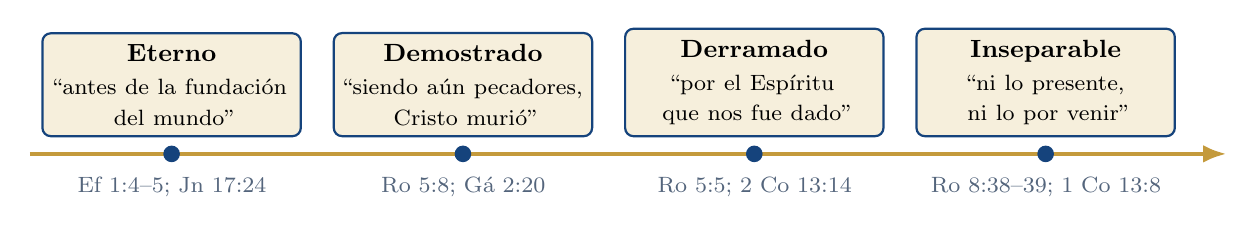
\begin{tikzpicture}[font=\small]
 \tikzset{hito/.style={draw=azul,line width=0.8pt,fill=papiro,rounded corners=3pt,text width=3.0cm,align=center,inner sep=4pt}}
 \draw[-{Latex[length=3mm]},dorado,line width=1.6pt] (0,0) -- (15.2,0);
 \foreach \x/\t/\r/\p in {0.9/Eterno/{antes de la fundación del mundo}/{Ef 1:4--5; Jn 17:24},
                          4.6/Demostrado/{siendo aún pecadores, Cristo murió}/{Ro 5:8; Gá 2:20},
                          8.3/Derramado/{por el Espíritu que nos fue dado}/{Ro 5:5; 2 Co 13:14},
                          12.0/Inseparable/{ni lo presente, ni lo por venir}/{Ro 8:38--39; 1 Co 13:8}} {
   \fill[azul] (\x+0.9,0) circle (3pt);
   \node[hito,above=6pt] at (\x+0.9,0) {\textbf{\t}\\[1pt]{\footnotesize ``\r''}};
   \node[below=5pt,text width=3.0cm,align=center,font=\footnotesize\color{gris}] at (\x+0.9,0) {\p};
 }
\end{tikzpicture}\par
{\footnotesize\color{gris}\textit{Figura 2.} El amor de Dios en Pablo: de antes del tiempo a más allá de la muerte. \textit{Nota.} Elaboración propia.}
\end{center}

\subsection{“El cual me amó y se entregó a sí mismo por mí”}
El amor eterno y soberano de Dios por un pueblo se vuelve, en Pablo, amor personal:

\begin{verso}{Gálatas 2:20}
Con Cristo estoy juntamente crucificado, y ya no vivo yo, mas vive Cristo en mí; y lo que ahora vivo en la carne, lo vivo en la fe del Hijo de Dios, el cual me amó y se entregó a sí mismo por mí.
\end{verso}

\begin{filologia}{Gá 2:20}
\grc{τοῦ ἀγαπήσαντός με} & \grc{ἀγαπάω} & ``que me amó'': aoristo, un acto concreto en la historia. Singular: Pablo, que había perseguido a la iglesia (Gá 1:13), se sabe amado en persona. \\
\grc{παραδόντος ἑαυτόν} & \grc{παραδίδωμι} & ``que se entregó a sí mismo'': el amor no da algo, se da. El mismo verbo describe al Padre que ``entregó'' al Hijo (Ro 8:32). \\
\end{filologia}

Lo mismo dice Pablo del amor de Cristo por la iglesia, con la imagen de Oseas: ``Maridos, amad a vuestras mujeres, así como Cristo amó a la iglesia, y se entregó a sí mismo por ella'' (Ef 5:25). El profeta compró a una esposa infiel (Os 3:1--2); Cristo se entregó por una esposa que no era santa para hacerla santa (Ef 5:26--27).

\precision{pablo no cita Oseas en Efesios 5; su texto explícito es Gn 2:24 (Ef 5:31). La relación con Oseas 3 es una lectura tipológica propia de esta serie, apoyada en que Pablo sí cita Oseas para hablar del amor que llama ``amada'' a la que no lo era (Ro 9:25; Os 2:23).}

\subsection{Los tres rasgos en Pablo}
\subsubsection*{Eterno}
``Según nos escogió en él antes de la fundación del mundo\ldots{} en amor habiéndonos predestinado'' (Ef 1:4--5). Pablo llama a los tesalonicenses ``hermanos amados por el Señor'', escogidos ``desde el principio'' (2 Ts 2:13), y alaba a ``Dios nuestro Padre, el cual nos amó y nos dio consolación eterna'' (2 Ts 2:16). El amor que precede al tiempo da una consolación que no se termina.

\subsubsection*{Soberano}
``Pero Dios, que es rico en misericordia, por su gran amor con que nos amó, aun estando nosotros muertos en pecados, nos dio vida juntamente con Cristo (por gracia sois salvos)'' (Ef 2:4--5). La única causa nombrada es ``su gran amor'' (\grc{διὰ τὴν πολλὴν ἀγάπην αὐτοῦ}). Tito lo dice con otra palabra: ``cuando se manifestó la bondad de Dios nuestro Salvador, y su amor para con los hombres (\grc{φιλανθρωπία}), nos salvó, no por obras de justicia que nosotros hubiéramos hecho'' (Tit 3:4--5).

\subsubsection*{Inmutable}
``Nada nos podrá separar'' (Ro 8:39) es la versión paulina de ``yo \SENOR{} no cambio; por esto, hijos de Jacob, no habéis sido consumidos'' (Mal 3:6). Y en el himno al amor, Pablo aplica al amor lo que Malaquías dijo de Dios: ``El amor nunca deja de ser'' (\grc{ἡ ἀγάπη οὐδέποτε πίπτει}, 1 Co 13:8), mientras profecías, lenguas y ciencia se acabarán.

\begin{center}\small\renewcommand{\arraystretch}{1.2}
\begin{tabular}{@{}L{2.2cm}L{4.2cm}L{4.2cm}L{4.2cm}@{}}
\toprule
\textbf{Rasgo} & \textbf{Escrituras de Israel} & \textbf{Pablo} & \textbf{Lo que muestra la cruz} \\ \midrule
Eterno & Jer 31:3; Os 11:1 & Ef 1:4--5; 2 Ts 2:13, 16 & El Hijo amado ``desde antes de la fundación del mundo'' es el que se entrega (Jn 17:24; Gá 2:20). \\
Soberano & Dt 7:7--8; 10:15; Mal 1:2; Os 14:4 & Ro 5:8; 9:13; Ef 2:4--5; Tit 3:4--5 & Cristo muere por débiles, impíos, pecadores y enemigos. \\
Inmutable & Mal 3:6; Os 11:8--9; Is 54:10; Cnt 8:7 & Ro 8:35--39; 1 Co 13:8 & Ni la muerte separa: el Amado resucitó y ``intercede por nosotros'' (Ro 8:34). \\
\bottomrule
\end{tabular}\par
{\footnotesize\color{gris}\textit{Tabla 6.} El amor eterno, soberano e inmutable, de Israel a Pablo. \textit{Nota.} Elaboración propia.}
\end{center}

\subsection{La plenitud del amor en Cristo}
``Para que, arraigados y cimentados en amor, seáis plenamente capaces de comprender con todos los santos cuál sea la anchura, la longitud, la profundidad y la altura, y de conocer el amor de Cristo, que excede a todo conocimiento, para que seáis llenos de toda la plenitud de Dios'' (Ef 3:17--19). Pablo ora para conocer lo que no se puede abarcar; Pink lo llama el amor ``infinito'' de Dios (Pink, 2020, p.~86). La oración termina en ``la plenitud de Dios'', la misma plenitud que ``habita corporalmente'' en Cristo (Col 2:9). Esa es la tesis de esta obra aplicada al amor: el amor que Dios es se ve entero en el Hijo, porque el Padre ama al Hijo desde siempre y en él ama a los suyos ``como también a mí me has amado'' (Jn 17:23).

%===================================================================
\section{Aplicación a la vida}

Juan saca la consecuencia en una frase: ``Amados, si Dios nos ha amado así, debemos también nosotros amarnos unos a otros'' (1 Jn 4:11). El amor de Dios es incomunicable como fuente, pero se comunica como reflejo. Cada rasgo tiene su eco en la vida del creyente.

\subsection{Porque es eterno: seguridad}
Un amor que no empezó con mi obediencia no depende de mi desempeño para seguir. ``En el amor no hay temor, sino que el perfecto amor echa fuera el temor'' (1 Jn 4:18). El creyente no sirve a Dios para ganar su amor, sino porque ya es amado: ``Nosotros le amamos a él, porque él nos amó primero'' (1 Jn 4:19).

\subsection{Porque es soberano: humildad y gratitud}
Si Dios no amó a Israel por ser numeroso, ni a nosotros por ser buenos, nadie puede gloriarse: ``¿qué tienes que no hayas recibido? Y si lo recibiste, ¿por qué te glorías como si no lo hubieras recibido?'' (1 Co 4:7). El amor soberano también enseña a amar sin condiciones previas. Deuteronomio funda el mandamiento en el carácter de Dios: Dios ``ama también al extranjero dándole pan y vestido. Amaréis, pues, al extranjero; porque extranjeros fuisteis en la tierra de Egipto'' (Dt 10:18--19). Jesús lo lleva al extremo: ``Amad a vuestros enemigos\ldots{} para que seáis hijos de vuestro Padre que está en los cielos'' (Mt 5:44--45).

\subsection{Porque es inmutable: perseverancia en la prueba}
La disciplina no contradice el amor: ``el Señor al que ama, disciplina'' (He 12:6). Pink advierte que ningún cristiano debe dudar del amor de Dios cuando sufre, porque el Padre amaba al Hijo y no lo eximió del sufrimiento (Pink, 2020, p.~87). Ante la tribulación, la pregunta de Pablo no es ``¿por qué?'', sino ``¿quién nos separará?'' (Ro 8:35). Judas resume la tarea: ``conservaos en el amor de Dios'' (Jud 21); el amor no se gana, pero se habita.

\subsection{Amar como él}
El amor que se pide al creyente tiene la forma del amor de Dios: ``Sed, pues, imitadores de Dios como hijos amados. Y andad en amor, como también Cristo nos amó, y se entregó a sí mismo por nosotros'' (Ef 5:1--2). Pablo lo resume con la Torá: ``el cumplimiento de la ley es el amor'' (Ro 13:10), citando ``Amarás a tu prójimo como a ti mismo'' (Lv 19:18; Ro 13:9). Y lo describe en 1 Corintios 13 con rasgos que, leídos de nuevo, son los del amor de Dios: ``El amor es sufrido, es benigno\ldots{} no guarda rencor\ldots{} Todo lo sufre, todo lo cree, todo lo espera, todo lo soporta. El amor nunca deja de ser'' (1 Co 13:4--8).

\begin{center}\small\renewcommand{\arraystretch}{1.2}
\begin{tabular}{@{}L{2.4cm}L{5.4cm}L{7.0cm}@{}}
\toprule
\textbf{Rasgo} & \textbf{En Dios} & \textbf{Reflejo en el creyente} \\ \midrule
Eterno & Amó antes de que existiéramos (Jer 31:3; Ef 1:4) & Seguridad sin temor (1 Jn 4:18--19) \\
Soberano & Amó sin causa en nosotros (Dt 7:7--8; Ro 5:8) & Humildad (1 Co 4:7) y amor al que no lo merece (Dt 10:19; Mt 5:44) \\
Inmutable & No deja de amar (Mal 3:6; Ro 8:39) & Perseverancia en la prueba (Ro 8:35; Jud 21) y un amor que ``nunca deja de ser'' (1 Co 13:8) \\
\bottomrule
\end{tabular}\par
{\footnotesize\color{gris}\textit{Tabla 7.} Del amor de Dios al amor del creyente. \textit{Nota.} Elaboración propia.}
\end{center}

\subsection{Conclusión}
El verso que une esta obra dice: ``alábese en esto el que se hubiere de alabar: en entenderme y conocerme, que yo soy \SENOR, que hago misericordia, juicio y justicia en la tierra; porque estas cosas quiero'' (Jer 9:24). Conocer a Dios como amor no es conocer un sentimiento, sino a una persona que ama desde siempre, sin causa fuera de sí y sin cambio. Ese amor se dejó ver en Moriah, en el Sinaí, en la casa de Oseas y, por último, en la cruz, donde el Padre ``no escatimó ni a su propio Hijo''. Por eso la confesión de Juan es también la de esta serie: ``nosotros hemos conocido y creído el amor que Dios tiene para con nosotros. Dios es amor'' (1 Jn 4:16).

%===================================================================

% \chapter{...}% Capítulo: Dios es Espíritu (generado desde ../03_Espiritu/03_Espiritu_capitulo.tex)
% Texto ancla: Juan 4:19–24. Clasificación: Ser; incomunicable en su esencia, comunicable como reflejo.

\section{Tres palabras en un pozo}

Es mediodía en Samaria. Jesús, ``cansado del camino'', se sienta junto al pozo de Jacob, y una mujer llega a sacar agua (Jn 4:6--7). La conversación empieza con agua y termina con una de las frases más densas de toda la Escritura:

\begin{verso}{Juan 4:24}
Dios es Espíritu; y los que le adoran, en espíritu y en verdad es necesario que adoren.
\end{verso}

En griego son tres palabras: \grc{πνεῦμα ὁ θεός}, ``espíritu (es) Dios''. No es una definición dicha en una escuela de filosofía, sino en una conversación sobre dónde se debe adorar. La mujer pregunta por un \destacar{lugar}, Gerizim o Jerusalén; Jesús responde con el \destacar{ser} de Dios. Porque Dios es Espíritu, el lugar deja de ser la pregunta. El atributo no se presenta como especulación: se presenta como la razón de una adoración nueva.

Esta serie agrupa en el Ser lo que responde a la pregunta ``¿qué es Dios?''. Juan da tres fórmulas con la misma forma: ``Dios es Espíritu'' (Jn 4:24), ``Dios es luz'' (1 Jn 1:5) y ``Dios es amor'' (1 Jn 4:8). Pink las reúne como las ``tres cosas que nos dicen las Escrituras con respecto a la naturaleza de Dios'' (Pink, 2020, cap. 16, p. 83).

\begin{center}
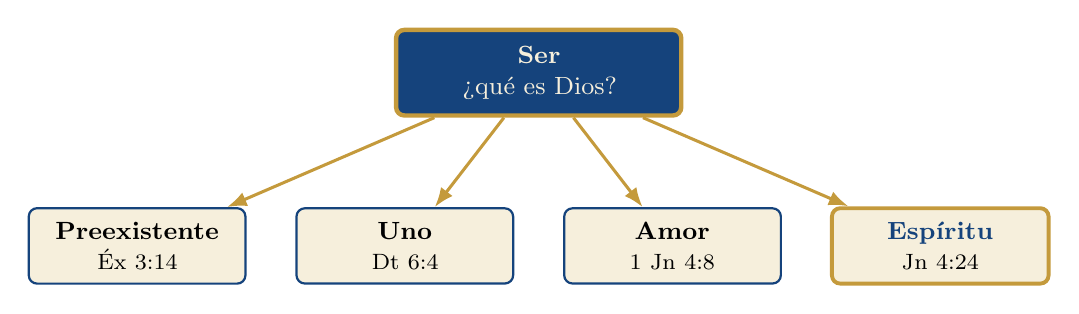
\begin{tikzpicture}[font=\small,
  caja/.style={draw=azul,line width=0.8pt,fill=papiro,rounded corners=3pt,inner sep=5pt,align=center}]
 \node[draw=dorado,line width=1.6pt,fill=azul,text=papiro,rounded corners=3pt,text width=3.2cm,align=center,inner sep=6pt] (s) at (0,1.9) {\textbf{Ser}\\ ¿qué es Dios?};
 \node[caja,text width=2.4cm] (p) at (-5.1,-0.3) {\textbf{Preexistente}\\ {\footnotesize Éx 3:14}};
 \node[caja,text width=2.4cm] (u) at (-1.7,-0.3) {\textbf{Uno}\\ {\footnotesize Dt 6:4}};
 \node[caja,text width=2.4cm] (a) at (1.7,-0.3) {\textbf{Amor}\\ {\footnotesize 1 Jn 4:8}};
 \node[draw=dorado,line width=1.4pt,fill=papiro,rounded corners=3pt,text width=2.4cm,align=center,inner sep=5pt] (e) at (5.1,-0.3) {\textbf{\textcolor{azul}{Espíritu}}\\ {\footnotesize Jn 4:24}};
 \foreach \i in {p,u,a,e}\draw[-{Latex[length=2.5mm]},dorado,line width=1.1pt](s)--(\i);
\end{tikzpicture}\par
{\footnotesize\color{gris}\textit{Figura 1.} El atributo dentro de la Parte I (Ser). \textit{Nota.} Elaboración propia según la clasificación de la serie.}
\end{center}

\precision{clasificación propuesta: atributo del Ser; \emph{incomunicable} en su esencia, porque Dios es espíritu increado, infinito y fuente de todo espíritu; \emph{comunicable} como reflejo, porque Dios ``forma el espíritu del hombre dentro de él'' (Zac 12:1).}

La palabra ``espíritu'' es de las más frecuentes de la Biblia. El conteo propio con la RVR1960 (sin títulos de sección, con números Strong) da estas cifras:

\begin{center}\small\renewcommand{\arraystretch}{1.18}
\begin{tabular}{@{}L{4.2cm}L{5.4cm}r@{}}
\toprule
\textbf{Forma (RVR1960)} & \textbf{Original más frecuente} & \textbf{Veces} \\ \midrule
espíritu & \heb{רוּחַ} \emph{rúaj}, \grc{πνεῦμα} \emph{pneûma} & 608 \\
espíritus & \heb{רוּחוֹת}, \grc{πνεύματα} & 36 \\
espiritual & \grc{πνευματικός} & 19 \\
espirituales & \grc{πνευματικός} & 10 \\
espiritualmente & \grc{πνευματικῶς} & 1 \\ \midrule
\textbf{Total} & \textbf{607 versículos (262 AT, 412 NT)} & \textbf{674} \\
\bottomrule
\end{tabular}\par
{\footnotesize\color{gris}\textit{Tabla 1.} ``Espíritu'' y sus formas en la RVR1960. \textit{Nota.} Conteo propio con la RVR1960 sin títulos de sección; los versículos del AT y del NT suman más de 607 porque se cuentan las apariciones por testamento. Verificar en e-Sword.}
\end{center}

El verso que une esta obra pide gloriarse en ``entenderme y conocerme'' (Jer 9:24 [9:23]). Saber que Dios es Espíritu es saber, ante todo, que no se le conoce como se conoce a una cosa: no se le ve, no se le toca, no se le encierra. Y, sin embargo, se le conoce, porque él habla y se acerca.

%===================================================================
\section{Texto ancla: Juan 4:19--24}

\subsection{Sicar, el pozo de Jacob}

\begin{verso}{Juan 4:5–6}
Vino, pues, a una ciudad de Samaria llamada Sicar, junto a la heredad que Jacob dio a su hijo José. Y estaba allí el pozo de Jacob.
\end{verso}

El diálogo ocurre en tierra de patriarcas. Allí Abram levantó su primer altar en Canaán, en ``el lugar de Siquem'' (Gn 12:6--7); allí Jacob compró un campo y erigió un altar al que llamó ``El-Elohe-Israel'' (Gn 33:18--20); frente a Siquem se alza Gerizim, el monte de la bendición (Dt 11:29; 27:12). Después de la caída de Samaria, los colonos traídos por Asiria ``temían a \SENOR, y honraban a sus dioses'' (2 R 17:24, 33). La pregunta de la mujer tiene siglos de historia.

\begin{center}
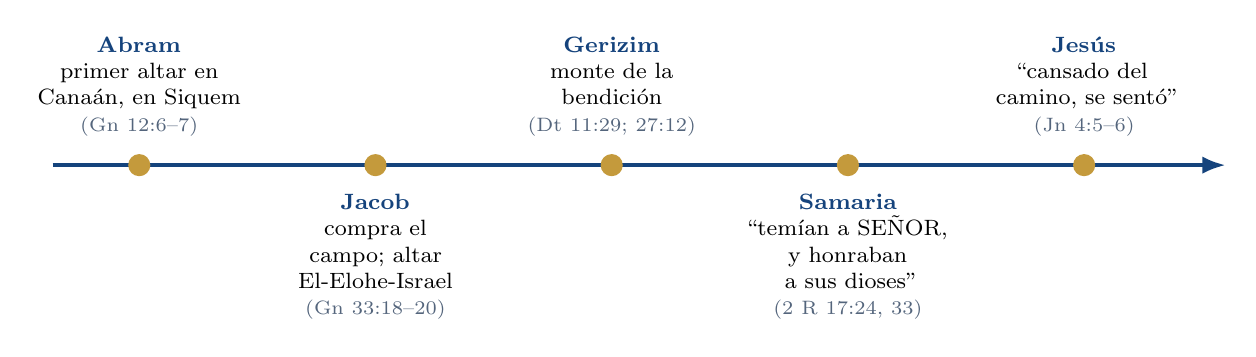
\begin{tikzpicture}[font=\footnotesize]
 \draw[line width=1.6pt,azul,-{Latex[length=3mm]}] (-0.3,0) -- (14.6,0);
 \foreach \x/\t/\b/\r/\pos in {0.8/{Abram}/{primer altar en Canaán, en Siquem}/{Gn 12:6--7}/above,
   3.8/{Jacob}/{compra el campo; altar El-Elohe-Israel}/{Gn 33:18--20}/below,
   6.8/{Gerizim}/{monte de la bendición}/{Dt 11:29; 27:12}/above,
   9.8/{Samaria}/{``temían a \SENOR, y honraban a sus dioses''}/{2 R 17:24, 33}/below,
   12.8/{Jesús}/{``cansado del camino, se sentó''}/{Jn 4:5--6}/above}{
  \fill[dorado] (\x,0) circle (4pt);
  \node[\pos=7pt,text width=2.6cm,align=center] at (\x,0) {\textbf{\textcolor{azul}{\t}}\\ \b\\ {\scriptsize\color{gris}(\r)}};}
\end{tikzpicture}\par
{\footnotesize\color{gris}\textit{Figura 2.} Siquem y Gerizim en la historia bíblica. \textit{Nota.} Elaboración propia.}
\end{center}

\subsection{``¿Este monte o Jerusalén?''}

\begin{verso}{Juan 4:19–20}
Le dijo la mujer: Señor, me parece que tú eres profeta. Nuestros padres adoraron en este monte, y vosotros decís que en Jerusalén es el lugar donde se debe adorar.
\end{verso}

Samaritanos y judíos compartían la Torá, pero no el lugar de culto. La disputa tenía base textual y una historia de violencia:

\begin{center}\small\renewcommand{\arraystretch}{1.22}
\begin{tabular}{@{}L{2.2cm}L{6.0cm}L{6.0cm}@{}}
\toprule
 & \textbf{Samaritanos: Gerizim} & \textbf{Judíos: Jerusalén} \\ \midrule
Canon & solo el Pentateuco & Ley, Profetas y Escritos \\
Base & altares de Abram y Jacob en Siquem (Gn 12:6--7; 33:20); la bendición en Gerizim (Dt 11:29; 27:12) & ``el lugar que \SENOR{} vuestro Dios escogiere'' (Dt 12:5), identificado con Sion (2 Cr 6:6; Sal 132:13) \\
Texto & el Pentateuco samaritano lee ``Gerizim'' en Dt 27:4 (TM: ``Ebal'') y añade Gerizim al Decálogo & el TM lee ``Ebal'' en Dt 27:4 \\
Templo & construido en Gerizim; destruido por Juan Hircano (129 a.\,e.\,c.) & segundo templo, en pie en tiempos de Jesús \\
\bottomrule
\end{tabular}\par
{\footnotesize\color{gris}\textit{Tabla 2.} La disputa sobre el lugar de culto. \textit{Nota.} Elaboración propia a partir de Tov (2012), la \emph{Encyclopaedia Judaica} (2007, ``Gerizim, Mount'') y MacArthur (2011, nota a Jn 4:20).}
\end{center}

\precision{(textual) las lecturas del Pentateuco samaritano siguen a Tov (2012). La \emph{Encyclopaedia Judaica} (2007) fecha la destrucción del templo de Gerizim en 129 a.\,e.\,c., según Josefo (\emph{Antigüedades} 13.255--256).}

\subsection{El texto}

\begin{verso}{Juan 4:21–24}
Jesús le dijo: Mujer, créeme, que la hora viene cuando ni en este monte ni en Jerusalén adoraréis al Padre. Vosotros adoráis lo que no sabéis; nosotros adoramos lo que sabemos; porque la salvación viene de los judíos. Mas la hora viene, y ahora es, cuando los verdaderos adoradores adorarán al Padre en espíritu y en verdad; porque también el Padre tales adoradores busca que le adoren. Dios es Espíritu; y los que le adoran, en espíritu y en verdad es necesario que adoren.
\end{verso}

\begin{filologia}{Jn 4:23--24}
\grc{ἔρχεται ὥρα καὶ νῦν ἐστιν} & \grc{ἔρχομαι} & ``viene la hora, y ahora es'': lo futuro ya empezó con Jesús (cf. Jn 5:25). \\
\grc{προσκυνέω} \emph{proskynéō} & \grc{κυνέω} & ``adorar'', postrarse; 9 veces en 4:20--24. La LXX lo usa para \heb{הִשְׁתַּחֲוָה} \emph{hishtajavá}, ``inclinarse'' (Éx 20:5). \\
\grc{πνεῦμα ὁ θεός} & \grc{πνέω} & ``Espíritu (es) Dios'': el predicado va primero y sin artículo; describe qué es Dios, no lo pone en una clase (``un espíritu''). \\
\grc{ἐν πνεύματι καὶ ἀληθείᾳ} & --- & una sola preposición para los dos sustantivos: una sola manera de adorar. \\
\grc{δεῖ} \emph{deî} & --- & ``es necesario'': el mismo verbo de la mujer en 4:20 (``donde se debe adorar''). Jesús cambia el dónde por el cómo. \\
\end{filologia}

Pink observa lo mismo sobre la gramática: ``En el griego, no hay un artículo indefinido y decir `Dios es un espíritu' es muy objetable, puesto que lo ubica en una clase con otros. Dios es `espíritu' en el sentido más elevado'' (Pink, 2020, cap. 16, p. 83).

\subsection{Del lugar a la manera}

El argumento de Jesús avanza en cuatro pasos. La mujer pregunta \emph{dónde} (4:20); Jesús anuncia una \emph{hora} en que ni este monte ni Jerusalén serán el centro (4:21); afirma la \emph{historia} de la revelación, porque ``la salvación viene de los judíos'' (4:22); y funda todo en el \emph{ser} de Dios (4:24).

\begin{center}
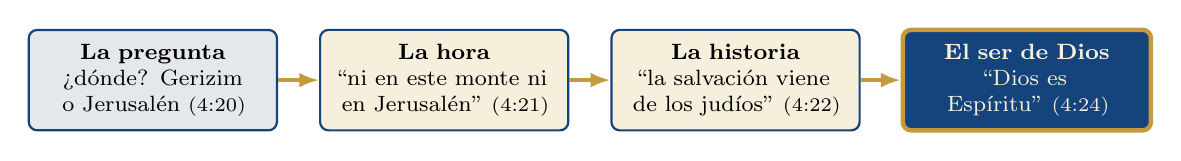
\begin{tikzpicture}[font=\footnotesize,
  caja/.style={draw=azul,line width=0.8pt,fill=papiro,rounded corners=3pt,inner sep=5pt,align=center,text width=2.8cm}]
 \node[caja,fill=gris!15] (a) at (0,0) {\textbf{La pregunta}\\ ¿dónde? Gerizim o Jerusalén {\scriptsize(4:20)}};
 \node[caja] (b) at (3.7,0) {\textbf{La hora}\\ ``ni en este monte ni en Jerusalén'' {\scriptsize(4:21)}};
 \node[caja] (c) at (7.4,0) {\textbf{La historia}\\ ``la salvación viene de los judíos'' {\scriptsize(4:22)}};
 \node[draw=dorado,line width=1.6pt,fill=azul,text=papiro,rounded corners=3pt,text width=2.8cm,align=center,inner sep=5pt] (d) at (11.1,0) {\textbf{El ser de Dios}\\ ``Dios es Espíritu'' {\scriptsize(4:24)}};
 \draw[-{Latex[length=2.5mm]},dorado,line width=1.2pt] (a)--(b); \draw[-{Latex[length=2.5mm]},dorado,line width=1.2pt] (b)--(c); \draw[-{Latex[length=2.5mm]},dorado,line width=1.2pt] (c)--(d);
\end{tikzpicture}\par
{\footnotesize\color{gris}\textit{Figura 3.} El argumento de Jn 4:20--24. \textit{Nota.} Elaboración propia.}
\end{center}

Jesús no relativiza la revelación: ``nosotros adoramos lo que sabemos''. La salvación tiene historia y pueblo. Pero el Dios de esa historia no está atado a un monte. Lo que estaba ligado a un lugar se liga ahora a una persona y a una manera. Y la iniciativa es de Dios: el Padre ``busca'' (\grc{ζητεῖ}) adoradores. Salomón ya lo había dicho al dedicar el templo:

\begin{verso}{1 Reyes 8:27}
Pero ¿es verdad que Dios morará sobre la tierra? He aquí que los cielos, los cielos de los cielos, no te pueden contener; ¿cuánto menos esta casa que yo he edificado?
\end{verso}

\subsection{``En espíritu y en verdad''}

La expresión se ha leído de dos maneras principales:

\begin{center}\small\renewcommand{\arraystretch}{1.22}
\begin{tabular}{@{}L{3.0cm}L{5.6cm}L{5.6cm}@{}}
\toprule
\textbf{Lectura} & \textbf{Sentido} & \textbf{Apoyo} \\ \midrule
Espíritu humano & adorar desde lo interior, no solo con ritos y lugares & MacArthur (2011, nota a Jn 4:24); Is 66:2, ``humilde de espíritu'' \\
Espíritu Santo & adorar movidos por el Espíritu que Jesús dará & Jn 3:5--6; 7:38--39: el agua viva ``dijo del Espíritu'' \\
``Verdad'' & conforme a la revelación, centrada en Jesús & Jn 1:14, 17; 14:6 \\
\bottomrule
\end{tabular}\par
{\footnotesize\color{gris}\textit{Tabla 3.} Lecturas de ``en espíritu y en verdad''. \textit{Nota.} Elaboración propia.}
\end{center}

En el mismo capítulo, Jesús había ofrecido a la mujer un agua distinta:

\begin{verso}{Juan 4:14}
mas el que bebiere del agua que yo le daré, no tendrá sed jamás; sino que el agua que yo le daré será en él una fuente de agua que salte para vida eterna.
\end{verso}

Y más adelante el evangelista explica qué es esa agua: ``Esto dijo del Espíritu que habían de recibir los que creyesen en él'' (Jn 7:39). La adoración ``en espíritu'' corresponde a lo que Dios \destacar{es}: el adorador debe ser semejante al adorado. Por eso el agua viva (4:14) y la adoración nueva (4:24) van juntas.

\precision{la referencia de ``espíritu'' en Jn 4:23--24 (espíritu humano o Espíritu Santo) se discute. El contexto de Juan, donde el agua viva es el Espíritu (7:39), favorece que el espíritu humano adore movido por el Espíritu de Dios. Es una lectura propia de esta serie.}

%===================================================================
\section{La palabra: \emph{rúaj}, viento, aliento, espíritu}

\subsection{Una palabra con cuatro rostros}

El hebreo no tiene una palabra para ``inmaterial''. Para decir lo que Dios es, usa una palabra concreta: \heb{רוּחַ} \emph{rúaj}, que dice a la vez viento, aliento y espíritu. Lo común a todos sus sentidos es algo \destacar{real, invisible y poderoso}. No se ve el viento, se ven sus efectos; no se ve el aliento, se ve la vida.

\begin{center}
\begin{tikzpicture}[font=\footnotesize,
  caja/.style={draw=azul,line width=0.8pt,fill=papiro,rounded corners=3pt,inner sep=5pt,align=center,text width=3.6cm}]
 \node[draw=dorado,line width=1.6pt,fill=azul,text=papiro,circle,minimum size=2cm,align=center] (c) at (0,0) {\heb{רוּחַ}\\ \emph{rúaj}};
 \node[caja] (v) at (-4.6,1.3) {\textbf{Viento}\\ ``por recio viento oriental'' {\scriptsize(Éx 14:21)}};
 \node[caja] (a) at (4.6,1.3) {\textbf{Aliento}\\ ``por el aliento de su boca'' {\scriptsize(Sal 33:6)}};
 \node[caja] (h) at (-4.6,-1.4) {\textbf{Vida, ánimo}\\ ``el espíritu vuelva a Dios que lo dio'' {\scriptsize(Ec 12:7)}};
 \node[caja] (e) at (4.6,-1.4) {\textbf{Espíritu de Dios}\\ ``el Espíritu de Dios se movía'' {\scriptsize(Gn 1:2)}};
 \foreach \i in {v,a,h,e}\draw[dorado,line width=1.1pt] (c)--(\i);
\end{tikzpicture}\par
{\footnotesize\color{gris}\textit{Figura 4.} Los sentidos de \emph{rúaj}. \textit{Nota.} Elaboración propia a partir de Vine (1999) y Chávez (1992).}
\end{center}

Vine (1999) agrupa los usos en aliento, aire fugaz, viento, ánimo y espíritu; Chávez (1992) distingue, entre ellos, el ``espíritu, distinto e independiente del factor material'' (Pr 16:2; Is 31:3).

\subsection{Génesis 1:2 y 2:7: el Espíritu que se cierne y el aliento que da vida}

\hebverso{וְרוּחַ אֱלֹהִים מְרַחֶפֶת עַל־פְּנֵי הַמָּיִם}
\begin{verso}{Génesis 1:2}
Y la tierra estaba desordenada y vacía, y las tinieblas estaban sobre la faz del abismo, y el Espíritu de Dios se movía sobre la faz de las aguas.
\end{verso}

\begin{filologia}{Gn 1:2}
\heb{רוּחַ אֱלֹהִים} \emph{rúaj Elohim} & \heb{רוח} & ``Espíritu de Dios''. Es la primera aparición de \emph{rúaj} en la Biblia: el Espíritu de Dios presente en la creación. \\
\heb{מְרַחֶפֶת} \emph{merajéfet} & \heb{רחף} & ``se cernía'', ``revoloteaba''. El mismo verbo describe al águila que ``revolotea sobre sus pollos'' (\heb{יְרַחֵף}, Dt 32:11). \\
\end{filologia}

\precision{la lectura de Gn 1:2 como ``viento de Dios'' es antigua. El Targum Ónkelos traduce \heb{וְרוּחָא מִן קֳדָם יְיָ מְנַשְּׁבָא}, ``y un viento de delante del \SENOR{} soplaba''. La RVR1960 lee ``Espíritu''.}

\hebverso{וַיִּפַּח בְּאַפָּיו נִשְׁמַת חַיִּים}
\begin{verso}{Génesis 2:7}
Entonces \SENOR{} Dios formó al hombre del polvo de la tierra, y sopló en su nariz aliento de vida, y fue el hombre un ser viviente.
\end{verso}

\begin{filologia}{Gn 2:7}
\heb{וַיִּפַּח} \emph{vayyipaj} & \heb{נפח} & ``y sopló'': el hombre vive porque Dios sopla. \\
\heb{נִשְׁמַת חַיִּים} \emph{nishmat jayyim} & \heb{נשׁם} & ``aliento de vida''. \emph{Neshamá} es ``aliento, hálito''; la RVR1960 la traduce ``espíritu'' en Job 26:4 y Pr 20:27: ``Lámpara de \SENOR{} es el espíritu del hombre''. \\
\end{filologia}

El mismo vocabulario sirve para la creación del cosmos y para la del hombre: ``Por la palabra de \SENOR{} fueron hechos los cielos, y todo el ejército de ellos por el aliento de su boca'' (Sal 33:6, \heb{וּבְרוּחַ פִּיו}). Lo que Dios dice y lo que Dios sopla dan existencia y vida.

\subsection{El espectro completo}

La tabla reúne el espectro completo: los términos hebreos, arameos y griegos que la RVR1960 traduce con ``espíritu'' y las palabras emparentadas.

\begin{center}\small\renewcommand{\arraystretch}{1.18}
\begin{tabular}{@{}L{3.3cm}L{3.3cm}L{4.0cm}L{3.6cm}@{}}
\toprule
\textbf{Término} & \textbf{Sentido} & \textbf{RVR1960} & \textbf{Textos} \\ \midrule
\heb{רוּחַ} \emph{rúaj} (H7307) & viento, aliento, ánimo, espíritu & espíritu ($\approx$\,200), viento(s) ($\approx$\,74), aliento, soplo, hálito, aire, lado & Gn 1:2; 8:1; Nm 16:22; Is 31:3; Ez 37:9 \\
\heb{רוּחַ} \emph{rúaj} (arameo, H7308) & viento; espíritu, mente & espíritu, viento & Dn 2:35; 4:8; 5:12; 7:15 \\
\heb{נְשָׁמָה} \emph{neshamá} (H5397) & soplo, aliento vital & aliento, espíritu, soplo & Gn 2:7; Job 26:4; Pr 20:27 \\
\heb{נֶפֶשׁ} \emph{néfesh} & aliento, vida, persona & ``amargura de espíritu'' (\heb{מַר־נֶפֶשׁ}) & 1 S 22:2 \\ \midrule
\grc{πνεῦμα} \emph{pneûma} (379) & viento, aliento, espíritu, Espíritu & espíritu, viento, aliento & Jn 3:8; 4:24; Ro 8:16; 2 Ts 2:8 \\
\grc{πνευματικός} (26) & espiritual & espiritual(es) & Ro 7:14; 1 Co 2:13--15; 15:44 \\
\grc{πνευματικῶς} (2) & espiritualmente & espiritualmente, en sentido espiritual & 1 Co 2:14; Ap 11:8 \\
\grc{πνοή} (2) & soplo, aliento & viento, aliento & Hch 2:2; 17:25 \\
\grc{πνέω} (7) & soplar & soplar & Jn 3:8; Hch 27:40 \\
\grc{ἐκπνέω} (3) & expirar & expirar & Mr 15:37; Lc 23:46 \\
\grc{θεόπνευστος} (1) & ``soplada por Dios'' & inspirada por Dios & 2 Ti 3:16 \\
\bottomrule
\end{tabular}\par
{\footnotesize\color{gris}\textit{Tabla 4.} Espectro hebreo, arameo y griego de ``espíritu''. \textit{Nota.} Conteo propio con la BHS y la NA27 (números Strong) y la RVR1960; los conteos por traducción son aproximados. Verificar en e-Sword.}
\end{center}

El conteo propio en la BHS da para \emph{rúaj} 376 apariciones en 349 versículos (366 en hebreo y 10 en arameo), con el etiquetado Strong incompleto; Vine (1999) da ``unas 378'' para el hebreo. Los libros donde más aparece son Ezequiel (51) e Isaías (49). No hay que confundirla con \heb{רָוַח} (1 S 16:23, ``tenía alivio''), de la misma raíz \emph{r-w-ḥ}, ``respirar, tener holgura''.

La Septuaginta traduce \emph{rúaj} casi siempre con \grc{πνεῦμα}, y el griego conserva el doble sentido. Jesús juega con él ante Nicodemo:

\begin{verso}{Juan 3:8}
El viento sopla de donde quiere, y oyes su sonido; mas ni sabes de dónde viene, ni a dónde va; así es todo aquel que es nacido del Espíritu.
\end{verso}

``El viento'' es \grc{τὸ πνεῦμα}; ``del Espíritu'' es \grc{ἐκ τοῦ πνεύματος}. La misma palabra dice las dos cosas.

\precision{\grc{φάντασμα} (``fantasma'', Mt 14:26; Mr 6:49) no se traduce ``espíritu''. En Lc 24:37 la RVR1960 traduce \grc{πνεῦμα} ``espíritu''.}

\subsection{``Carne, y no espíritu''}

El texto del Antiguo Testamento que más se acerca a Jn 4:24 no está en un salmo, sino en una advertencia política. Judá buscaba ayuda militar en Egipto, y confiaba en sus carros y caballos (Is 31:1). Isaías responde:

\hebverso{וּמִצְרַיִם אָדָם וְלֹא־אֵל \\ וְסוּסֵיהֶם בָּשָׂר וְלֹא־רוּחַ}
\begin{verso}{Isaías 31:3}
Y los egipcios hombres son, y no Dios; y sus caballos carne, y no espíritu; de manera que al extender \SENOR{} su mano, caerá el ayudador y caerá el ayudado, y todos ellos desfallecerán a una.
\end{verso}

El paralelismo es exacto: hombre // carne; Dios // espíritu. Isaías opone la \destacar{carne} perecedera al \destacar{espíritu} que pertenece a Dios. Lo que se ve y se cuenta (caballos, carros, ejércitos) es lo débil; lo que no se ve es lo fuerte.

\begin{center}
\begin{tikzpicture}[font=\small,
  caja/.style={draw=azul,line width=0.8pt,fill=gris!15,rounded corners=3pt,inner sep=5pt,align=center,text width=2.6cm},
  dios/.style={draw=dorado,line width=1.4pt,fill=azul,text=papiro,rounded corners=3pt,inner sep=5pt,align=center,text width=2.6cm}]
 \node[caja] (a) at (0,1.2) {\heb{אָדָם} hombre};
 \node[dios] (b) at (5,1.2) {\heb{אֵל} Dios};
 \node[caja] (c) at (0,0) {\heb{בָּשָׂר} carne};
 \node[dios] (d) at (5,0) {\heb{רוּחַ} espíritu};
 \draw[<->,gris,thick] (a)--(b) node[midway,above,font=\footnotesize]{no es};
 \draw[<->,gris,thick] (c)--(d) node[midway,above,font=\footnotesize]{no es};
\end{tikzpicture}\par
{\footnotesize\color{gris}\textit{Figura 5.} El paralelismo de Is 31:3. \textit{Nota.} Elaboración propia.}
\end{center}

\precision{(textual) la LXX no tiene ``y no espíritu'': lee \grc{καὶ οὐκ ἔστιν βοήθεια}, ``y no hay ayuda''. El Targum conserva \heb{בְּסַר וְלָא רוּחַ}.}

\subsection{Los ídolos: forma sin espíritu}

Si Dios es espíritu sin forma, el ídolo es lo contrario: forma sin espíritu.

\begin{verso}{Jeremías 10:14}
Todo hombre se embrutece, y le falta ciencia; se avergüenza de su ídolo todo fundidor, porque mentirosa es su obra de fundición, y no hay espíritu en ella.
\end{verso}

\begin{verso}{Habacuc 2:19}
¡Ay del que dice al palo: Despiértate; y a la piedra muda: Levántate! ¿Podrá él enseñar? He aquí está cubierto de oro y plata, y no hay espíritu dentro de él.
\end{verso}

En hebreo, \heb{וְלֹא־רוּחַ בָּם} (Jer 10:14) y \heb{וְכָל־רוּחַ אֵין בְּקִרְבּוֹ} (Hab 2:19). El Salmo lo dice del aliento: ``Tampoco hay aliento en sus bocas'' (Sal 135:17, \heb{רוּחַ}). El ídolo tiene boca y no respira; el Dios verdadero no tiene forma visible y es todo vida.

\precision{jer 10:14 pertenece al texto ancla del atributo Verdadero (Jer 10:1--16): allí el ídolo es mentira porque no tiene espíritu.}

%===================================================================
\section{El Nombre que revela su ser espiritual}

\subsection{``Dios de los espíritus de toda carne''}

El Antiguo Testamento no tiene un nombre propio ``Espíritu'' para Dios. Tiene, en cambio, un título que aparece dos veces en Números, siempre en boca de Moisés y siempre en oración:

\hebverso{אֵל אֱלֹהֵי הָרוּחֹת לְכָל־בָּשָׂר}
\begin{verso}{Números 16:22}
Y ellos se postraron sobre sus rostros, y dijeron: Dios, Dios de los espíritus de toda carne, ¿no es un solo hombre el que pecó? ¿Por qué airarte contra toda la congregación?
\end{verso}

\begin{verso}{Números 27:16}
Ponga \SENOR, Dios de los espíritus de toda carne, un varón sobre la congregación.
\end{verso}

\begin{filologia}{Nm 16:22}
\heb{אֵל אֱלֹהֵי} & \heb{אל} & ``Dios, Dios de\ldots'': vocativo doble en la oración de Moisés y Aarón. \\
\heb{הָרוּחֹת} \emph{harujot} & \heb{רוח} & ``los espíritus'', plural de \emph{rúaj}: el aliento vital de cada ser humano. \\
\heb{לְכָל־בָּשָׂר} & \heb{בשׂר} & ``de toda carne'': toda criatura viviente. \\
LXX & --- & \grc{θεὸς θεὸς τῶν πνευμάτων καὶ πάσης σαρκός}: ``Dios de los espíritus y de toda carne''. \\
Ónkelos & --- & \heb{אֵל אֱלָהּ רוּחַיָּא לְכָל בִּשְׂרָא}: conserva la fórmula. \\
\end{filologia}

Las dos veces la fórmula aparece en una situación límite. En Nm 16, tras la rebelión de Coré, Moisés apela al Dios que conoce cada espíritu para que no castigue a toda la congregación por el pecado de unos pocos. En Nm 27, al acercarse su muerte, pide al mismo Dios un sucesor: Josué. El Dios de los espíritus juzga con justicia porque conoce el interior de cada uno, y provee pastores porque sabe lo que cada uno necesita.

Rashi lo entendió así en ambos textos:

\begin{quote}\itshape
``Conoce los pensamientos'' (\heb{יוֹדֵעַ מַחֲשָׁבוֹת}). Un rey de carne y sangre, si una provincia peca contra él, no sabe quién pecó y castiga a todos; ``pero tú, ante ti están revelados todos los pensamientos''.\par\hfill{\upshape\small\bfseries\textcolor{azul}{(Rashi a Nm 16:22)}}
\end{quote}

\begin{quote}\itshape
``Manifiesto ante ti es el pensamiento de cada uno, y no se parecen entre sí''; pon sobre ellos un guía que soporte a cada uno según su manera de pensar.\par\hfill{\upshape\small\bfseries\textcolor{azul}{(Rashi a Nm 27:16)}}
\end{quote}

\precision{comentario rabínico medieval (Sefaria); traducción propia.}

\subsection{El que forma y da el espíritu}

Los profetas desarrollan el título en forma de participios: Dios es ``el que da aliento al pueblo que mora sobre ella, y espíritu a los que por ella andan'' (Is 42:5), y el que ``forma el espíritu del hombre dentro de él'':

\begin{verso}{Zacarías 12:1}
Profecía de la palabra de \SENOR{} acerca de Israel. \SENOR, que extiende los cielos y funda la tierra, y forma el espíritu del hombre dentro de él, ha dicho:
\end{verso}

El Nuevo Testamento recoge la fórmula: ``¿Por qué no obedeceremos mucho mejor al Padre de los espíritus, y viviremos?'' (He 12:9).

\begin{center}\small\renewcommand{\arraystretch}{1.22}
\begin{tabular}{@{}L{4.3cm}L{4.6cm}L{2.0cm}L{3.4cm}@{}}
\toprule
\textbf{Nombre o título} & \textbf{Hebreo / griego} & \textbf{Texto} & \textbf{Qué revela} \\ \midrule
Dios de los espíritus de toda carne & \heb{אֱלֹהֵי הָרוּחֹת לְכָל־בָּשָׂר} & Nm 16:22; 27:16 & dueño y conocedor de todo espíritu \\
El que forma el espíritu del hombre & \heb{יֹצֵר רוּחַ־אָדָם} & Zac 12:1 & fuente del espíritu humano \\
El que da aliento y espíritu & \heb{נֹתֵן נְשָׁמָה}\ldots{} \heb{וְרוּחַ} & Is 42:5 & dador de la vida \\
Padre de los espíritus & \grc{τῷ πατρὶ τῶν πνευμάτων} & He 12:9 & relación paternal \\
Dios de los espíritus de los profetas & \grc{ὁ θεὸς τῶν πνευμάτων τῶν προφητῶν} & Ap 22:6 & el que habla por los profetas \\
El Invisible & \grc{τὸν ἀόρατον} & He 11:27 & no se le ve, pero sostiene \\
\bottomrule
\end{tabular}\par
{\footnotesize\color{gris}\textit{Tabla 5.} Los nombres y títulos que revelan que Dios es Espíritu. \textit{Nota.} Elaboración propia.}
\end{center}

\precision{no hay un nombre propio ``Espíritu'' en el Antiguo Testamento. Se usa el título ``Dios de los espíritus'', que lo revela como fuente y dueño de todo espíritu. El Nombre que revela el atributo es, en esta serie, Nm 16:22, como se anunció en el mapa de los nombres de la Introducción.}

%===================================================================
\section{Definición}

\begin{tcolorbox}[colback=papiro,colframe=azul,boxrule=1pt,arc=3pt,title={Definición},colbacktitle=azul,coltitle=papiro]
Que Dios es Espíritu es la perfección eterna de su ser por la cual Dios existe sin cuerpo, sin partes y sin forma visible; es vida en sí mismo y fuente de toda vida; no está limitado por lugar ni puede ser representado por imagen; y se da a conocer por su palabra, por su Espíritu y, en plenitud, en el Hijo hecho carne.
\end{tcolorbox}

\precision{definición de síntesis de esta serie, a partir de los textos estudiados.}

La definición reúne seis rasgos, cada uno con su base bíblica:

\begin{center}\small\renewcommand{\arraystretch}{1.22}
\begin{tabular}{@{}L{3.6cm}L{10.6cm}@{}}
\toprule
\textbf{Rasgo} & \textbf{Texto} \\ \midrule
Incorpóreo & ``un espíritu no tiene carne ni huesos, como veis que yo tengo'' (Lc 24:39) \\
Invisible & ``al Rey de los siglos, inmortal, invisible, al único y sabio Dios'' (1 Ti 1:17) \\
Vivo y vivificante & ``El espíritu es el que da vida; la carne para nada aprovecha'' (Jn 6:63) \\
Sin límite de lugar & ``¿A dónde me iré de tu Espíritu?'' (Sal 139:7) \\
Sin imagen & ``ninguna figura visteis el día que \SENOR{} habló con vosotros'' (Dt 4:15) \\
Personal & ``el Padre tales adoradores busca que le adoren'' (Jn 4:23) \\
\bottomrule
\end{tabular}\par
{\footnotesize\color{gris}\textit{Tabla 6.} Los rasgos del atributo. \textit{Nota.} Elaboración propia.}
\end{center}

\subsection{Lo que no significa}

Decir que Dios es Espíritu puede entenderse mal. Cinco malentendidos frecuentes, y lo que responde la Escritura:

\begin{center}\small\renewcommand{\arraystretch}{1.25}
\begin{tabular}{@{}L{4.0cm}L{10.2cm}@{}}
\toprule
\textbf{Malentendido} & \textbf{Respuesta bíblica} \\ \midrule
``Un espíritu entre otros'' & Es ``Padre de los espíritus'' (He 12:9); los demás espíritus son criaturas (Zac 12:1). \\
Fuerza impersonal, energía & Habla, busca, ama: ``el Padre tales adoradores busca'' (Jn 4:23). \\
Irreal, vago, lejano & Es lo más real: ``las cosas que se ven son temporales, pero las que no se ven son eternas'' (2 Co 4:18). \\
Hostil a lo material & Creó la materia y la llamó ``bueno en gran manera'' (Gn 1:31); en Cristo habita ``corporalmente'' (Col 2:9). \\
Solo ``el Espíritu Santo'' & ``Dios es Espíritu'' dice qué es Dios (Padre, Hijo y Espíritu); ``el Espíritu Santo'' es una de las personas. \\
\bottomrule
\end{tabular}\par
{\footnotesize\color{gris}\textit{Tabla 7.} Malentendidos sobre el atributo. \textit{Nota.} Elaboración propia.}
\end{center}

\subsection{Manos, ojos, alas: el lenguaje de los hombres}

La Biblia describe a Dios con imágenes del cuerpo: ``al extender \SENOR{} su mano'' (Is 31:3); ``los ojos de \SENOR{} contemplan toda la tierra'' (2 Cr 16:9); ``bajo sus alas estarás seguro'' (Sal 91:4); ``El cielo es mi trono'' (Is 66:1). Son \emph{antropomorfismos}: lenguaje humano para hablar del poder, el cuidado y el gobierno de Dios. Las imágenes son verdaderas \emph{como imágenes}: Dios realmente actúa, ve y protege; pero no tiene miembros. La misma Torá que dice ``mano'' prohíbe hacer una figura de Dios (Dt 4:15--16).

Los sabios lo resumieron en una frase que Maimónides hizo clásica:

\hebverso{דִּבְּרָה תוֹרָה כִּלְשׁוֹן בְּנֵי אָדָם}
\begin{quote}\itshape
``La Torá habló en el lenguaje de los hombres''.\par\hfill{\upshape\small\bfseries\textcolor{azul}{(Berajot 31b, citado por Maimónides, Yesodé haTorá 1:9)}}
\end{quote}

\precision{el principio rabínico se cita según Maimónides, \emph{Mishné Torá}, Yesodé haTorá 1:9, y su comentario a la Misná, Sanedrín 10:1 (Sefaria).}

%===================================================================
\section{Teología: Pink y el Dios que es Espíritu}

\subsection{Incorpóreo, y por eso presente en todo lugar}

Pink no dedica un capítulo propio a este atributo, pero lo pone como la primera de las ``tres cosas'' que la Escritura dice de la naturaleza de Dios, y saca de él una consecuencia:

\begin{quote}\itshape
Debido a que es ``espíritu'', es incorpóreo, no tiene sustancia visible. Si Dios tuviera un cuerpo tangible, no sería omnipresente, estaría limitado a un lugar; pero precisamente porque es ``espíritu'', llena el cielo y la tierra.\par\hfill{\upshape\small\bfseries\textcolor{azul}{(Pink, 2020, cap. 16, p. 83)}}
\end{quote}

El Salmo 139 dice lo mismo con el paralelismo hebreo:

\hebverso{אָנָה אֵלֵךְ מֵרוּחֶךָ וְאָנָה מִפָּנֶיךָ אֶבְרָח}
\begin{verso}{Salmo 139:7–8}
¿A dónde me iré de tu Espíritu? ¿Y a dónde huiré de tu presencia? Si subiere a los cielos, allí estás tú; Y si en el Seol hiciere mi estrado, he aquí, allí tú estás.
\end{verso}

``Tu Espíritu'' // ``tu presencia'' (\heb{פָּנֶיךָ}, literalmente ``tu rostro''). Porque es Espíritu, Dios no ocupa un lugar: está en todo lugar. ``¿No lleno yo, dice \SENOR, el cielo y la tierra?'' (Jer 23:24). Lo que en Jn 4 suprime el monte, en el Salmo 139 suprime la huida. Este rasgo se estudiará en el atributo \emph{Omnipresente}.

\subsection{Invisible, pero revelado}

\begin{verso}{Éxodo 33:20}
Dijo más: No podrás ver mi rostro; porque no me verá hombre, y vivirá.
\end{verso}

\begin{verso}{1 Timoteo 6:16}
el único que tiene inmortalidad, que habita en luz inaccesible; a quien ninguno de los hombres ha visto ni puede ver, al cual sea la honra y el imperio sempiterno. Amén.
\end{verso}

Ningún ser humano ``ha visto ni puede ver'' a Dios: no por distancia, sino por lo que Dios es. Pink cita este mismo texto al presentar a Dios ``independiente de todo'', y añade que ese Dios ``sólo puede ser conocido cuando es revelado al corazón por el Espíritu Santo, a través de la Palabra''. Y lo funda en Jn 4:24:

\begin{quote}\itshape
Tampoco Dios es conocido por el intelecto. Dios es Espíritu (Jn. 4:24) y, por lo tanto, sólo puede ser conocido espiritualmente.\par\hfill{\upshape\small\bfseries\textcolor{azul}{(Pink, 2020, cap. 1, p. 9)}}
\end{quote}

Para Pink, el conocimiento salvador viene cuando el Espíritu Santo resplandece ``en nuestros corazones (y no en nuestros intelectos)'' para dar ``el conocimiento de la gloria de Dios en la faz de Jesucristo'' (2 Co 4:6). El Dios invisible no es un Dios mudo: Moisés no vio su rostro, pero oyó su Nombre (Éx 34:5--7).

\precision{la autoría paulina de 1 Timoteo se discute; la misma idea aparece en cartas indiscutidas: ``las cosas invisibles de él, su eterno poder y deidad'' (Ro 1:20).}

\subsection{Espíritu que da vida}

\hebverso{מֵאַרְבַּע רוּחוֹת בֹּאִי הָרוּחַ}
\begin{verso}{Ezequiel 37:9}
Y me dijo: Profetiza al espíritu, profetiza, hijo de hombre, y dí al espíritu: Así ha dicho \SENOR{} el Señor: Espíritu, ven de los cuatro vientos, y sopla sobre estos muertos, y vivirán.
\end{verso}

``De los cuatro \emph{rujot} ven, \emph{rúaj}'': viento, aliento y Espíritu en una sola frase. Y Dios explica la visión: ``Y pondré mi Espíritu en vosotros, y viviréis'' (Ez 37:14, \heb{רוּחִי}). El Dios que es Espíritu es vivo y da vida; Jesús lo dirá con palabras semejantes: ``El espíritu es el que da vida; la carne para nada aprovecha; las palabras que yo os he hablado son espíritu y son vida'' (Jn 6:63). Los ídolos no tienen \emph{rúaj} (Jer 10:14); el Dios vivo la \emph{da}.

\subsection{Un reflejo en el ser humano}

Dios \destacar{dio} espíritu al ser humano (Gn 2:7; Zac 12:1; Ec 12:7): por eso el atributo es comunicable como reflejo. Pablo usa la analogía para hablar del conocimiento de Dios:

\begin{verso}{1 Corintios 2:11}
Porque ¿quién de los hombres sabe las cosas del hombre, sino el espíritu del hombre que está en él? Así tampoco nadie conoció las cosas de Dios, sino el Espíritu de Dios.
\end{verso}

Como el espíritu del hombre conoce lo íntimo del hombre, solo el Espíritu de Dios conoce lo íntimo de Dios. Pero la analogía tiene un límite: el espíritu humano es dado, limitado y unido a un cuerpo; el de Dios es increado. ``El polvo vuelva a la tierra, como era, y el espíritu vuelva a Dios que lo dio'' (Ec 12:7).

\precision{1 Co 2:10--11 es el texto que este libro usa como marco de humildad: lo profundo de Dios solo lo conoce su Espíritu, y lo conocemos porque ``Dios nos las reveló a nosotros por el Espíritu'' (1 Co 2:10).}

%===================================================================
\section{Un encuentro en la historia de Israel: Horeb, una voz sin figura}

\subsection{``Ninguna figura visteis''}

Cuarenta años después del Sinaí, en las llanuras de Moab, Moisés recuerda a la nueva generación lo que sus padres vivieron al pie del monte. El centro del recuerdo es lo que Israel \emph{no} vio:

\hebverso{קוֹל דְּבָרִים אַתֶּם שֹׁמְעִים וּתְמוּנָה אֵינְכֶם רֹאִים זוּלָתִי קוֹל}
\begin{verso}{Deuteronomio 4:12}
y habló \SENOR{} con vosotros de en medio del fuego; oísteis la voz de sus palabras, mas a excepción de oír la voz, ninguna figura visteis.
\end{verso}

\begin{verso}{Deuteronomio 4:15}
Guardad, pues, mucho vuestras almas; pues ninguna figura visteis el día que \SENOR{} habló con vosotros de en medio del fuego;
\end{verso}

\begin{filologia}{Dt 4:12--18}
\heb{קוֹל דְּבָרִים} & \heb{קול} & ``voz de palabras'': Israel recibió palabras, no una imagen. \\
\heb{תְּמוּנָה} \emph{temuná} & \heb{מין} & ``figura, forma visible''. Lo que Israel no vio. \\
\heb{פֶּסֶל} \emph{pésel} & \heb{פסל} & ``escultura, imagen tallada'' (4:16). \\
\heb{סֶמֶל} \emph{sémel} & --- & ``efigie, estatua'' (4:16). \\
\heb{תַּבְנִית} \emph{tavnit} & \heb{בנה} & ``figura, modelo'': de varón, hembra, animal, ave, reptil, pez (4:16--18). \\
LXX 4:12 & --- & \grc{ὁμοίωμα οὐκ εἴδετε ἀλλ’ ἢ φωνήν}: ``semejanza no visteis, sino una voz''. \\
\end{filologia}

Moisés saca la consecuencia: como no hubo figura, no se hará figura. ``Para que no os corrompáis y hagáis para vosotros escultura, imagen de figura alguna, efigie de varón o hembra'' (Dt 4:16). La forma de la revelación (una voz sin imagen) corresponde al ser de Dios (Espíritu sin cuerpo).

\subsection{El becerro y la voz}

Entre Horeb y Moab ocurrió la caída. Al pie del mismo monte donde Dios se había revelado como voz, Israel quiso un dios que se \emph{viera}: Aarón hizo ``un becerro de fundición. Entonces dijeron: Israel, estos son tus dioses, que te sacaron de la tierra de Egipto'' (Éx 32:4). El Salmo lo recuerda con una frase amarga:

\begin{verso}{Salmo 106:19–20}
Hicieron becerro en Horeb, Se postraron ante una imagen de fundición. Así cambiaron su gloria Por la imagen de un buey que come hierba.
\end{verso}

\begin{center}
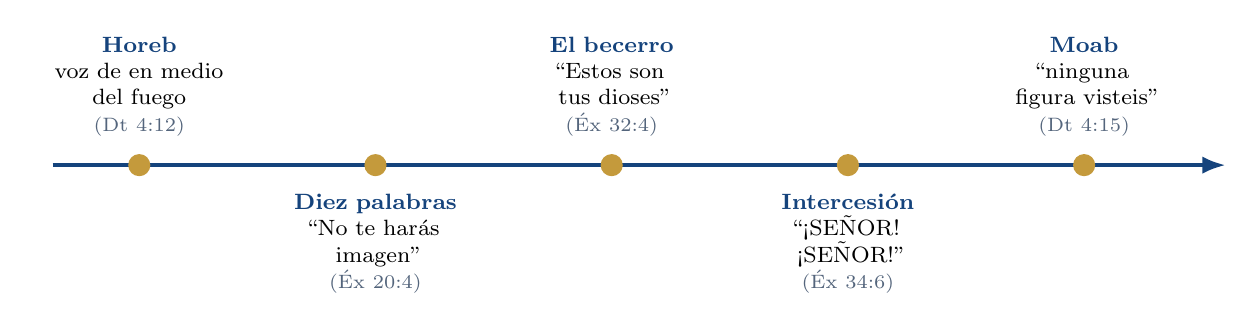
\begin{tikzpicture}[font=\footnotesize]
 \draw[line width=1.6pt,azul,-{Latex[length=3mm]}] (-0.3,0) -- (14.6,0);
 \foreach \x/\t/\b/\r/\pos in {0.8/{Horeb}/{voz de en medio del fuego}/{Dt 4:12}/above,
   3.8/{Diez palabras}/{``No te harás imagen''}/{Éx 20:4}/below,
   6.8/{El becerro}/{``Estos son tus dioses''}/{Éx 32:4}/above,
   9.8/{Intercesión}/{``¡\SENOR! ¡\SENOR!''}/{Éx 34:6}/below,
   12.8/{Moab}/{``ninguna figura visteis''}/{Dt 4:15}/above}{
  \fill[dorado] (\x,0) circle (4pt);
  \node[\pos=7pt,text width=2.6cm,align=center] at (\x,0) {\textbf{\textcolor{azul}{\t}}\\ \b\\ {\scriptsize\color{gris}(\r)}};}
\end{tikzpicture}\par
{\footnotesize\color{gris}\textit{Figura 6.} De Horeb a Moab. \textit{Nota.} Elaboración propia.}
\end{center}

La idolatría empieza por querer ver. Dios respondió al becerro no con una imagen, sino con su Nombre proclamado: ``¡\SENOR! ¡\SENOR! fuerte, misericordioso y piadoso'' (Éx 34:6). Aun en el perdón, se dio a conocer por palabra.

\subsection{La lista de figuras, en Pablo}

La lista de Dt 4:16--18 reaparece, siglos después, en la carta a los Romanos. Pablo describe la idolatría humana con el vocabulario de la Septuaginta:

\begin{center}\small\renewcommand{\arraystretch}{1.2}
\begin{tabular}{@{}L{3.6cm}L{5.2cm}L{5.2cm}@{}}
\toprule
\textbf{Dt 4:16--18} & \textbf{LXX} & \textbf{Ro 1:23} \\ \midrule
figura, efigie & \grc{ὁμοίωμα}, \grc{εἰκών} & \grc{ἐν ὁμοιώματι εἰκόνος} \\
varón o hembra & \grc{ἀρσενικοῦ ἢ θηλυκοῦ} & \grc{φθαρτοῦ ἀνθρώπου} \\
animal de la tierra & \grc{κτήνους} & \grc{τετραπόδων} \\
ave alada & \grc{ὀρνέου πτερωτοῦ} & \grc{πετεινῶν} \\
lo que se arrastra & \grc{ἑρπετοῦ} & \grc{ἑρπετῶν} \\
\bottomrule
\end{tabular}\par
{\footnotesize\color{gris}\textit{Tabla 8.} Dt 4:16--18 y Ro 1:23. \textit{Nota.} Elaboración propia con la LXX de Rahlfs-Hanhart y NA28.}
\end{center}

\begin{verso}{Romanos 1:23}
y cambiaron la gloria del Dios incorruptible en semejanza de imagen de hombre corruptible, de aves, de cuadrúpedos y de reptiles.
\end{verso}

``Cambiaron la gloria'' (\grc{ἤλλαξαν τὴν δόξαν}) es también el lenguaje del Sal 106:20 en la LXX (\grc{ἠλλάξαντο τὴν δόξαν}). Lo que Horeb prohibió, el mundo lo hizo.

\precision{el eco de Dt 4:16--18 y Sal 106:20 en Ro 1:23 es lectura de varios intérpretes (cf. Dunn, 1998); se apoya en el vocabulario común de la LXX.}

%===================================================================
\section{Dios es Espíritu en el judaísmo}\label{sec:judaismo-esp}

\subsection{El alma y el Santo}

El Talmud pregunta por qué David dijo cinco veces ``Bendice, alma mía, a \SENOR'' (Sal 103--104). Rabí Yehoshúa ben Leví responde que el alma se parece al Santo, bendito sea:

\hebverso{מָה הַקָּדוֹשׁ בָּרוּךְ הוּא רוֹאֶה וְאֵינוֹ נִרְאֶה \\ אַף נְשָׁמָה רוֹאָה וְאֵינָהּ נִרְאֵית}
\begin{quote}\itshape
``Como el Santo, bendito sea, ve y no es visto, así el alma ve y no es vista''.\par\hfill{\upshape\small\bfseries\textcolor{azul}{(Talmud de Babilonia, Berajot 10a)}}
\end{quote}

\begin{center}\small\renewcommand{\arraystretch}{1.2}
\begin{tabular}{@{}L{5.6cm}L{5.6cm}@{}}
\toprule
\textbf{El Santo} & \textbf{El alma} \\ \midrule
llena todo el mundo & llena todo el cuerpo \\
ve y no es visto & ve y no es vista \\
sustenta el mundo & sustenta el cuerpo \\
es puro & es pura \\
mora en lo más íntimo & mora en lo más íntimo \\
\bottomrule
\end{tabular}\par
{\footnotesize\color{gris}\textit{Tabla 9.} Las cinco semejanzas de \emph{Berajot} 10a. \textit{Nota.} Elaboración propia a partir del Talmud (edición William Davidson, Sefaria).}
\end{center}

Y concluye: ``Venga quien tiene estas cinco cosas y alabe al que tiene estas cinco cosas''.

\precision{interpretación rabínica (Talmud de Babilonia, edición William Davidson, Sefaria); traducción propia. Es una analogía: el alma es criatura, Dios no.}

\subsection{Maimónides: ``no es cuerpo''}

Para Maimónides, la incorporeidad de Dios no es un detalle filosófico, sino parte de la fe misma de Israel. En su comentario a la Misná (Sanedrín 10:1) la pone como el tercero de sus trece principios, ``la negación de la corporeidad'': Dios ``no es cuerpo ni fuerza en un cuerpo''; y la funda en Dt 4:15, \heb{כִּי לֹא רְאִיתֶם כָּל תְּמוּנָה}. En el \emph{Mishné Torá} lo dice así:

\hebverso{שֶׁאֵין הַקָּדוֹשׁ בָּרוּךְ הוּא גּוּף וּגְוִיָּה}
\begin{quote}\itshape
``El Santo, bendito sea, no es cuerpo ni figura''; y un cuerpo no puede estar en dos lugares.\par\hfill{\upshape\small\bfseries\textcolor{azul}{(Maimónides, Yesodé haTorá 1:8)}}
\end{quote}

En las leyes del arrepentimiento (Teshuvá 3:7) cuenta entre los herejes (\emph{minim}) al que dice que hay un solo Señor, ``pero que es cuerpo y tiene figura''. Y recoge la enseñanza de \emph{Jaguigá} 15a: ``arriba no hay sentarse ni estar de pie''.

La liturgia lo canta cada mañana. El himno \emph{Yigdal}, basado en los trece principios, dice:

\hebverso{אֵין לוֹ דְמוּת הַגּוּף וְאֵינוֹ גוּף}
\begin{quote}\itshape
``No tiene semejanza de cuerpo, ni es cuerpo''.\par\hfill{\upshape\small\bfseries\textcolor{azul}{(\emph{Yigdal}, oración de la mañana)}}
\end{quote}

\precision{lecturas judías medievales; el \emph{Yigdal} se atribuye a Daniel ben Yehudá de Roma (siglo XIV). Textos según Sefaria; traducción propia.}

\subsection{\emph{Rúaj} en la \emph{Guía de los perplejos}}

En la \emph{Guía} (I:40), Maimónides abre con una advertencia: \heb{רוּחַ שֵׁם מִשְׁתַּתֵּף}, ``\emph{rúaj} es un nombre equívoco'', de varios sentidos. Distingue seis:

\begin{center}\small\renewcommand{\arraystretch}{1.18}
\begin{tabular}{@{}L{0.6cm}L{5.6cm}L{8.0cm}@{}}
\toprule
& \textbf{Sentido} & \textbf{Texto que cita} \\ \midrule
1 & el aire, uno de los cuatro elementos & ``el Espíritu de Dios se movía'' (Gn 1:2) \\
2 & el viento que sopla & ``el viento oriental trajo la langosta'' (Éx 10:13) \\
3 & el espíritu vital & ``soplo que va y no vuelve'' (Sal 78:39); Gn 7:15 \\
4 & lo que queda del hombre después de la muerte & ``el espíritu vuelva a Dios que lo dio'' (Ec 12:7) \\
5 & la influencia intelectual divina sobre los profetas & ``tomaré del espíritu que está en ti'' (Nm 11:17); 2 S 23:2 \\
6 & la intención, la voluntad & ``¿Quién enseñó al Espíritu de \SENOR?'' (Is 40:13) \\
\bottomrule
\end{tabular}\par
{\footnotesize\color{gris}\textit{Tabla 10.} Los sentidos de \emph{rúaj} en Maimónides, \emph{Guía de los perplejos} I:40. \textit{Nota.} Elaboración propia a partir de la versión hebrea de Samuel ibn Tibbon (Sefaria).}
\end{center}

Todo \emph{rúaj} atribuido a Dios es, para él, el sentido 5 o el 6.

\precision{versión hebrea de Samuel ibn Tibbon (Sefaria); traducción propia. La lectura filosófica de Maimónides, que entiende el Espíritu como ``influencia'', no coincide con la lectura cristiana del Espíritu como persona.}

\subsection{Los targumes y Rashi: la gloria, la voz}

Las traducciones arameas evitan decir que alguien \emph{vio} a Dios. Donde el hebreo dice ``y vieron al Dios de Israel'' (Éx 24:10), Ónkelos traduce \heb{וַחֲזוֹ יָת יְקַר אֱלָהָא דְיִשְׂרָאֵל}, ``y vieron \emph{la gloria} del Dios de Israel''. En Dt 4:12 lee \heb{וּדְמוּת לֵיתֵיכוֹן חָזָן אֶלָּהֵן קָלָא}, ``y semejanza no veis, sino la voz''. Es la misma convicción de Deuteronomio.

Rashi, en Gn 1:2, explica la imagen de la creación sin darle cuerpo a Dios: ``el trono de gloria estaba en el aire y se cernía sobre las aguas por el aliento de su boca'' (\heb{בְּרוּחַ פִּיו}), ``como paloma que se cierne sobre el nido''.

\precision{interpretaciones judías antiguas y medievales (Sefaria); traducción propia.}

\subsection{Qumrán: espíritu y verdad}

La \emph{Regla de la Comunidad} de Qumrán (1QS) enseña que Dios puso en el hombre ``dos espíritus'', el de la verdad y el de la falsedad, hasta el tiempo de su visita (1QS III 17--19). Al final, Dios purificará al hombre con ``espíritu de santidad'' y rociará sobre él ``el espíritu de verdad como aguas de purificación'' (1QS IV 20--21). Espíritu, verdad y agua: las tres palabras de Jn 4:14, 23--24 aparecen juntas en un texto judío anterior al evangelio.

\precision{paráfrasis según García Martínez (1992) y Vermes (2004); conviene cotejar en la Leon Levy Dead Sea Scrolls Digital Library. La relación con Juan es un paralelo de lenguaje, no una dependencia demostrada.}

%===================================================================
\section{Dios es Espíritu en Cristo, leído con Pablo}\label{sec:cristo-esp}

\subsection{La imagen del Dios invisible}

Israel no podía hacer una imagen de Dios porque en Horeb no vio ninguna figura. Pablo, judío formado en Dt 4 y en Is 31, no hace imágenes de Dios. Pero confiesa que Dios mismo tiene una imagen, y que no la hizo el hombre:

\begin{verso}{Colosenses 1:15}
El es la imagen del Dios invisible, el primogénito de toda creación.
\end{verso}

\begin{verso}{Colosenses 2:9}
Porque en él habita corporalmente toda la plenitud de la Deidad,
\end{verso}

\begin{filologia}{Col 1:15 y 2:9}
\grc{εἰκὼν τοῦ θεοῦ τοῦ ἀοράτου} & \grc{εἰκών} & ``imagen del Dios invisible'': la misma palabra de Ro 1:23 (\grc{εἰκόνος}), ahora para el Hijo. \\
\grc{κατοικεῖ} & \grc{οἰκέω} & ``habita'' de modo permanente. \\
\grc{σωματικῶς} & \grc{σῶμα} & ``corporalmente'': la plenitud de la Deidad, que no tiene cuerpo, habita en un cuerpo. \\
\end{filologia}

La única ``imagen'' legítima de Dios es el Hijo. El Dios que es Espíritu, sin cuerpo, habita en plenitud en un \destacar{cuerpo}. Esto no niega Jn 4:24: lo cumple. Dios no se hizo visible renunciando a ser Espíritu, sino uniendo a sí una humanidad verdadera.

\precision{la autoría paulina de Colosenses se discute; la misma idea aparece en una carta indiscutida: Cristo, ``el cual es la imagen de Dios'' (2 Co 4:4).}

\subsection{Deuteronomio 4 cumplido: Dios se deja ver}

\begin{verso}{Juan 1:18}
A Dios nadie le vio jamás; el unigénito Hijo, que está en el seno del Padre, él le ha dado a conocer.
\end{verso}

``Le ha dado a conocer'' es \grc{ἐξηγήσατο}: ``lo explicó, lo narró''. El Hijo es la exégesis del Padre. El que dijo ``no me verá hombre, y vivirá'' (Éx 33:20) se deja ver en el Hijo: ``El que me ha visto a mí, ha visto al Padre'' (Jn 14:9). Y Pablo lo dice en su propio lenguaje: Dios ``resplandeció en nuestros corazones, para iluminación del conocimiento de la gloria de Dios en la faz de Jesucristo'' (2 Co 4:6).

\begin{center}
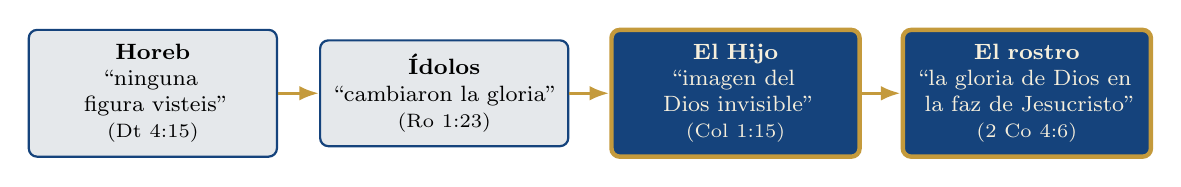
\begin{tikzpicture}[font=\footnotesize,
  caja/.style={draw=azul,line width=0.8pt,fill=gris!15,rounded corners=3pt,inner sep=5pt,align=center,text width=2.8cm},
  luz/.style={draw=dorado,line width=1.6pt,fill=azul,text=papiro,rounded corners=3pt,inner sep=5pt,align=center,text width=2.8cm}]
 \node[caja] (a) at (0,0) {\textbf{Horeb}\\ ``ninguna figura visteis''\\ {\scriptsize(Dt 4:15)}};
 \node[caja] (b) at (3.7,0) {\textbf{Ídolos}\\ ``cambiaron la gloria''\\ {\scriptsize(Ro 1:23)}};
 \node[luz] (c) at (7.4,0) {\textbf{El Hijo}\\ ``imagen del Dios invisible''\\ {\scriptsize(Col 1:15)}};
 \node[luz] (d) at (11.1,0) {\textbf{El rostro}\\ ``la gloria de Dios en la faz de Jesucristo''\\ {\scriptsize(2 Co 4:6)}};
 \draw[-{Latex[length=2.5mm]},dorado,line width=1.2pt] (a)--(b); \draw[-{Latex[length=2.5mm]},dorado,line width=1.2pt] (b)--(c); \draw[-{Latex[length=2.5mm]},dorado,line width=1.2pt] (c)--(d);
\end{tikzpicture}\par
{\footnotesize\color{gris}\textit{Figura 7.} Del Dios sin figura al rostro de Cristo. \textit{Nota.} Elaboración propia.}
\end{center}

\precision{(textual) en Jn 1:18 la NA28 lee \grc{μονογενὴς θεός}, ``el unigénito Dios''; la RVR1960 sigue el texto bizantino \grc{ὁ μονογενὴς υἱός}, ``el unigénito Hijo''.}

\subsection{``El Señor es el Espíritu''}

\begin{verso}{2 Corintios 3:16–18}
Pero cuando se conviertan al Señor, el velo se quitará. Porque el Señor es el Espíritu; y donde está el Espíritu del Señor, allí hay libertad. Por tanto, nosotros todos, mirando a cara descubierta como en un espejo la gloria del Señor, somos transformados de gloria en gloria en la misma imagen, como por el Espíritu del Señor.
\end{verso}

Pablo cita Éx 34:34 casi palabra por palabra:

\begin{center}\small\renewcommand{\arraystretch}{1.22}
\begin{tabular}{@{}L{2.0cm}L{7.0cm}L{5.2cm}@{}}
\toprule
\textbf{Texto} & \textbf{Original} & \textbf{RVR1960} \\ \midrule
Éx 34:34 TM & \heb{וּבְבֹא מֹשֶׁה לִפְנֵי יְהוָה}\ldots{} \heb{יָסִיר אֶת־הַמַּסְוֶה} & ``Cuando venía Moisés delante de \SENOR\ldots{} se quitaba el velo'' \\
Éx 34:34 LXX & \grc{ἡνίκα δ’ ἂν εἰσεπορεύετο Μωυσῆς ἔναντι κυρίου\ldots{} περιῃρεῖτο τὸ κάλυμμα} & --- \\
2 Co 3:16 & \grc{ἡνίκα δὲ ἐὰν ἐπιστρέψῃ πρὸς κύριον, περιαιρεῖται τὸ κάλυμμα} & ``cuando se conviertan al Señor, el velo se quitará'' \\
2 Co 3:17 & \grc{ὁ δὲ κύριος τὸ πνεῦμά ἐστιν} & ``el Señor es el Espíritu'' \\
\bottomrule
\end{tabular}\par
{\footnotesize\color{gris}\textit{Tabla 11.} Éx 34:34 en 2 Co 3:16--17. \textit{Nota.} Elaboración propia con la BHS, la LXX y NA28.}
\end{center}

El ``Señor'' (\grc{κύριος}) ante quien Moisés se quitaba el velo es el \SENOR{} del Sinaí. Pablo explica que ese \SENOR{} se encuentra hoy ``en el Espíritu'': el velo se quita cuando uno se vuelve al Señor que es Espíritu. El Dios que en Horeb habló sin figura es el que ahora, por su Espíritu, transforma a los suyos ``en la misma imagen'': la imagen del Hijo.

\precision{``El Señor es el Espíritu'' no confunde al Hijo con el Espíritu: es una exégesis de Éx 34, donde ``el Señor'' del texto se refiere al Espíritu que vivifica (2 Co 3:6). Lectura sostenida por Dunn (1998) y Hays (1989).}

\subsection{Pablo en Atenas}

Ante los filósofos de Atenas, Pablo predica al Dios que es Espíritu con el lenguaje de Israel:

\begin{verso}{Hechos 17:24–25}
El Dios que hizo el mundo y todas las cosas que en él hay, siendo Señor del cielo y de la tierra, no habita en templos hechos por manos humanas, ni es honrado por manos de hombres, como si necesitase de algo; pues él es quien da a todos vida y aliento y todas las cosas.
\end{verso}

\begin{verso}{Hechos 17:29}
Siendo, pues, linaje de Dios, no debemos pensar que la Divinidad sea semejante a oro, o plata, o piedra, escultura de arte y de imaginación de hombres.
\end{verso}

``No en templos hechos de mano'' (\grc{οὐκ ἐν χειροποιήτοις ναοῖς}) recoge a Salomón (1 R 8:27) y a Isaías (66:1); ``aliento'' (\grc{πνοή}) recoge el soplo de Gn 2:7 e Is 42:5. Y la prohibición de imaginar a Dios ``semejante a oro, o plata, o piedra'' es Dt 4 predicado a griegos.

\precision{el discurso fue transmitido por Lucas; se usa aquí como testimonio de la predicación de Pablo.}

\subsection{El nuevo templo: ni Gerizim ni Jerusalén}

\begin{verso}{Efesios 2:18, 22}
porque por medio de él los unos y los otros tenemos entrada por un mismo Espíritu al Padre\ldots{} en quien vosotros también sois juntamente edificados para morada de Dios en el Espíritu.
\end{verso}

\begin{verso}{1 Corintios 3:16}
¿No sabéis que sois templo de Dios, y que el Espíritu de Dios mora en vosotros?
\end{verso}

Lo que Jesús anunció en Sicar (``ni en este monte ni en Jerusalén'') Pablo lo ve cumplido: el templo es un pueblo, y Dios lo habita \grc{ἐν πνεύματι}, ``en el Espíritu''. Samaritanos y judíos discutían por un monte; Pablo ve a judíos y gentiles, ``los unos y los otros'', con acceso ``por un mismo Espíritu al Padre''. Es la adoración ``al Padre'' de Jn 4:21, 23.

\begin{center}
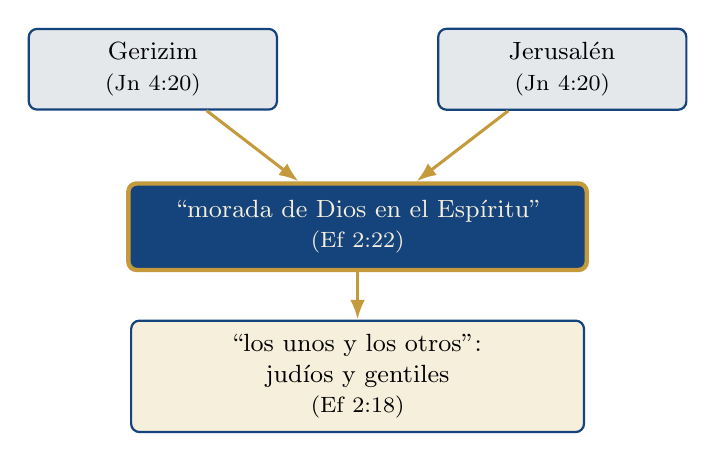
\begin{tikzpicture}[font=\small,
  caja/.style={draw=azul,line width=0.8pt,fill=papiro,rounded corners=3pt,inner sep=5pt,align=center}]
 \node[caja,text width=2.8cm,fill=gris!15] (g) at (-2.6,2.0) {Gerizim\\ {\footnotesize(Jn 4:20)}};
 \node[caja,text width=2.8cm,fill=gris!15] (j) at (2.6,2.0) {Jerusalén\\ {\footnotesize(Jn 4:20)}};
 \node[draw=dorado,line width=1.6pt,fill=azul,text=papiro,rounded corners=3pt,text width=5.4cm,align=center,inner sep=6pt] (t) at (0,0) {``morada de Dios en el Espíritu''\\ {\footnotesize(Ef 2:22)}};
 \node[caja,text width=5.4cm] (p) at (0,-1.9) {``los unos y los otros'': judíos y gentiles\\ {\footnotesize(Ef 2:18)}};
 \draw[-{Latex[length=2.5mm]},dorado,line width=1.1pt](g)--(t); \draw[-{Latex[length=2.5mm]},dorado,line width=1.1pt](j)--(t); \draw[-{Latex[length=2.5mm]},dorado,line width=1.1pt](t)--(p);
\end{tikzpicture}\par
{\footnotesize\color{gris}\textit{Figura 8.} Del monte al pueblo: la morada en el Espíritu. \textit{Nota.} Elaboración propia.}
\end{center}

\precision{la autoría paulina de Efesios se discute; 1 Co 3:16 dice lo mismo en una carta indiscutida.}

\subsection{``En espíritu servimos a Dios''}

\begin{verso}{Filipenses 3:3}
Porque nosotros somos la circuncisión, los que en espíritu servimos a Dios y nos gloriamos en Cristo Jesús, no teniendo confianza en la carne.
\end{verso}

\begin{verso}{Romanos 12:1}
Así que, hermanos, os ruego por las misericordias de Dios, que presentéis vuestros cuerpos en sacrificio vivo, santo, agradable a Dios, que es vuestro culto racional.
\end{verso}

Pablo usa el vocabulario del culto del templo: \grc{λατρεύοντες} (Flp 3:3) y \grc{λατρεία} (Ro 12:1). Opone ``espíritu'' a ``carne'' (Flp 3:3), como Is 31:3. Pero el culto nuevo no suprime el cuerpo: lo ofrece entero. El ``culto racional'' (\grc{λογικὴν λατρείαν}) es la adoración de Jn 4:24 vivida en lo cotidiano.

\precision{(textual) en Flp 3:3, NA28 y el texto bizantino leen \grc{πνεύματι θεοῦ λατρεύοντες}, ``los que servimos por el Espíritu de Dios''; la RVR1960 sigue la lectura ``servimos a Dios''.}

\subsection{``¡Abba, Padre!''}

\begin{verso}{Romanos 8:15–16}
Pues no habéis recibido el espíritu de esclavitud para estar otra vez en temor, sino que habéis recibido el espíritu de adopción, por el cual clamamos: ¡Abba, Padre! El Espíritu mismo da testimonio a nuestro espíritu, de que somos hijos de Dios.
\end{verso}

Jesús habló de adorar ``al Padre'' (Jn 4:21, 23); Pablo muestra cómo: el Espíritu nos hace decir ``Abba''. \grc{αὐτὸ τὸ πνεῦμα συμμαρτυρεῖ τῷ πνεύματι ἡμῶν}: el Espíritu de Dios testifica \emph{con} nuestro espíritu. Espíritu con espíritu: es la comunión que Jn 4:24 pide. Y esa comunión alcanza al cuerpo: ``si el Espíritu de aquel que levantó de los muertos a Jesús mora en vosotros, el que levantó de los muertos a Cristo Jesús vivificará también vuestros cuerpos mortales por su Espíritu que mora en vosotros'' (Ro 8:11).

\subsection{El postrer Adán, espíritu vivificante}

\begin{verso}{1 Corintios 15:45}
Así también está escrito: Fue hecho el primer hombre Adán alma viviente; el postrer Adán, espíritu vivificante.
\end{verso}

\begin{filologia}{1 Co 15:45 y Gn 2:7}
Gn 2:7 LXX & --- & \grc{ἐγένετο ὁ ἄνθρωπος εἰς ψυχὴν ζῶσαν}: ``fue el hombre un alma viviente''. \\
1 Co 15:45 & --- & \grc{ὁ ἔσχατος Ἀδὰμ εἰς πνεῦμα ζῳοποιοῦν}: ``el postrer Adán, espíritu que da vida''. \\
\grc{πνευματικόν} & \grc{πνεῦμα} & ``espiritual'' (15:44): el cuerpo de resurrección no es inmaterial, sino animado por el Espíritu. \\
\end{filologia}

El primer Adán \destacar{recibió} aliento (Gn 2:7); el último Adán \destacar{da} vida. Cristo resucitado hace lo que solo el Dios que es Espíritu hace: vivificar (Ez 37:14; Jn 6:63).

\subsection{Síntesis paulina}

\begin{center}
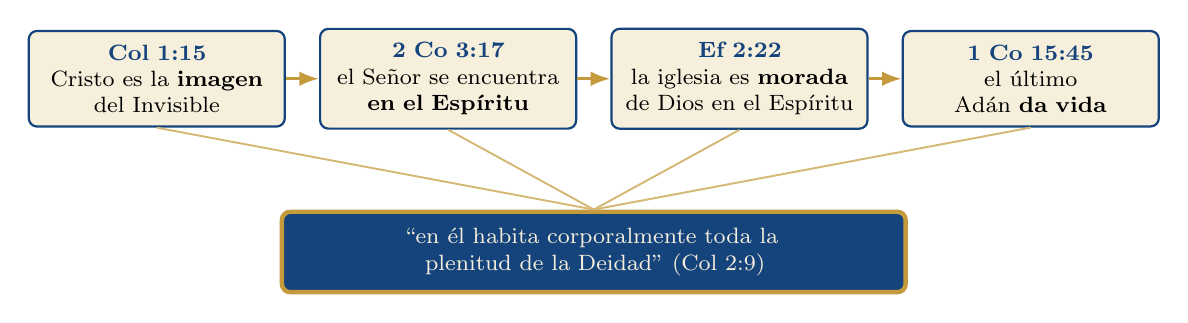
\begin{tikzpicture}[font=\footnotesize,
  caja/.style={draw=azul,line width=0.8pt,fill=papiro,rounded corners=3pt,inner sep=5pt,align=center,text width=2.9cm}]
 \node[caja] (a) at (0,0) {\textbf{\textcolor{azul}{Col 1:15}}\\ Cristo es la \textbf{imagen} del Invisible};
 \node[caja] (b) at (3.7,0) {\textbf{\textcolor{azul}{2 Co 3:17}}\\ el Señor se encuentra \textbf{en el Espíritu}};
 \node[caja] (c) at (7.4,0) {\textbf{\textcolor{azul}{Ef 2:22}}\\ la iglesia es \textbf{morada} de Dios en el Espíritu};
 \node[caja] (d) at (11.1,0) {\textbf{\textcolor{azul}{1 Co 15:45}}\\ el último Adán \textbf{da vida}};
 \draw[-{Latex[length=2.5mm]},dorado,line width=1.1pt](a)--(b); \draw[-{Latex[length=2.5mm]},dorado,line width=1.1pt](b)--(c); \draw[-{Latex[length=2.5mm]},dorado,line width=1.1pt](c)--(d);
 \node[draw=dorado,line width=1.6pt,fill=azul,text=papiro,rounded corners=3pt,text width=7.5cm,align=center,inner sep=6pt] (e) at (5.55,-2.2) {``en él habita corporalmente toda la plenitud de la Deidad'' (Col 2:9)};
 \foreach \i in {a,b,c,d}\draw[dorado!70,line width=0.7pt](\i.south)--(e.north);
\end{tikzpicture}\par
{\footnotesize\color{gris}\textit{Figura 9.} Dios es Espíritu, revelado en Cristo. \textit{Nota.} Elaboración propia.}
\end{center}

El Dios que es Espíritu se da a conocer en el Hijo y se da a sí mismo en el Espíritu. La tesis de esta obra (la plenitud de los atributos habita en Cristo, Col 2:9) tiene aquí una forma particular: la plenitud de un Dios sin cuerpo habita ``corporalmente'' en Jesús.

%===================================================================
\section{Aplicación: adorar al Dios que es Espíritu}

Jesús no dijo ``Dios es Espíritu'' para describir a Dios en abstracto, sino para responder cómo se le adora. La aplicación nace del mismo texto.

\subsection{Adorar sin monte}

\begin{verso}{Isaías 66:1–2}
\SENOR{} dijo así: El cielo es mi trono, y la tierra estrado de mis pies; ¿dónde está la casa que me habréis de edificar, y dónde el lugar de mi reposo?\ldots{} pero miraré a aquel que es pobre y humilde de espíritu, y que tiembla a mi palabra.
\end{verso}

Los lugares sirven, pero no contienen a Dios. El \SENOR{} mira al ``humilde de espíritu'' (\heb{נְכֵה־רוּחַ}). Ningún edificio, ritual o emoción garantiza la adoración; tampoco la impiden. ``Mas tú, cuando ores, entra en tu aposento, y cerrada la puerta, ora a tu Padre que está en secreto; y tu Padre que ve en lo secreto te recompensará en público'' (Mt 6:6).

\subsection{Sin imágenes, ni de piedra ni de la mente}

\begin{verso}{Isaías 40:18}
¿A qué, pues, haréis semejante a Dios, o qué imagen le compondréis?
\end{verso}

``¿Qué semejanza le pondréis?'' (\heb{וּמַה־דְּמוּת תַּעַרְכוּ לוֹ}). Hoy pocos tallan ídolos, pero muchos se forman un dios a su medida: un Dios solo ``útil'', solo ``cercano'' o solo ``lejano''. Conocemos a Dios por lo que \emph{dice} de sí mismo (Dt 4:12) y por el Hijo (Jn 1:18), no por lo que imaginamos. ``Hijitos, guardaos de los ídolos'' (1 Jn 5:21).

\subsection{Cuatro respuestas}

\begin{enumerate}
\item \textbf{Adorar} en espíritu y en verdad, en cualquier lugar y con toda la vida: ``que presentéis vuestros cuerpos en sacrificio vivo'' (Jn 4:24; Ro 12:1).
\item \textbf{Escuchar}: Dios se da a conocer por su palabra, no por imágenes. En Horeb hubo ``voz de palabras'' y ninguna figura (Dt 4:12).
\item \textbf{Andar} conducidos por su Espíritu, no por la carne: ``Andad en el Espíritu, y no satisfagáis los deseos de la carne'' (Gá 5:16); ``Si vivimos por el Espíritu, andemos también por el Espíritu'' (Gá 5:25).
\item \textbf{Esperar}: el Espíritu que mora en nosotros ``vivificará también vuestros cuerpos mortales'' (Ro 8:11). El Dios que sopló en el polvo (Gn 2:7) y sobre los huesos secos (Ez 37:9) soplará otra vez.
\end{enumerate}

Como atributo, ser Espíritu es incomunicable: solo Dios es espíritu increado, infinito y fuente de toda vida. Pero es comunicable como reflejo: Dios formó el espíritu del hombre dentro de él (Zac 12:1), y por su Espíritu lo hace capaz de adorarle. Las preguntas que deja el atributo son personales:

\begin{itemize}
\item ¿Dónde está hoy mi ``monte'': el lugar, el estilo o la emoción sin los que creo que no puedo adorar?
\item ¿Qué imagen de Dios me he formado que no viene de su palabra?
\item ¿Mi culto se queda en la reunión, o llega a mi cuerpo y a mi semana (Ro 12:1)?
\item ¿Vivo como quien tiene en sí el Espíritu del Dios vivo (Ro 8:11)?
\end{itemize}

%===================================================================
\section{Síntesis}

\begin{tcolorbox}[colback=papiro,colframe=azul,boxrule=1pt,arc=3pt]
``Dios es Espíritu'' (Jn 4:24). La palabra hebrea \emph{rúaj} une viento, aliento y espíritu: lo invisible que es real y da vida. Dios es el ``Dios de los espíritus de toda carne'' (Nm 16:22): sin cuerpo, sin figura, presente en todo lugar y fuente de toda vida. En Horeb se reveló como voz sin figura (Dt 4:12), y por eso Israel no debía hacer imágenes. En Sicar, Jesús dejó atrás la disputa de los montes: el Padre busca adoradores en espíritu y en verdad. Pablo lo ve cumplido: Cristo es ``la imagen del Dios invisible'' (Col 1:15), en él habita la plenitud ``corporalmente'' (Col 2:9), y la iglesia es ``morada de Dios en el Espíritu'' (Ef 2:22).
\end{tcolorbox}

\begin{center}\small\renewcommand{\arraystretch}{1.3}
\begin{tabular}{@{}L{3.0cm}L{11.4cm}@{}}
\toprule
\textbf{Mirada} & \textbf{Aporte al atributo} \\ \midrule
Hebrea & \emph{rúaj} (viento, aliento, espíritu); ``carne, y no espíritu'' (Is 31:3); voz sin figura (Dt 4:12); ``Dios de los espíritus de toda carne'' (Nm 16:22); los ídolos sin \emph{rúaj} (Jer 10:14). \\
Judía & El alma y el Santo (\emph{Berajot} 10a); ``no es cuerpo'' (Maimónides; \emph{Yigdal}); la Torá habla en lenguaje humano; los targumes: ``la gloria'', ``la voz''; Qumrán: espíritu de verdad y aguas. \\
Pink & No ``un espíritu'' entre otros; incorpóreo y por eso omnipresente; conocido solo espiritualmente, por revelación. \\
Paulina & Imagen del Invisible (Col 1:15); ``el Señor es el Espíritu'' (2 Co 3:17); templo en el Espíritu (Ef 2:22); culto racional (Ro 12:1); ``¡Abba, Padre!'' (Ro 8:15); el postrer Adán da vida (1 Co 15:45). \\
\bottomrule
\end{tabular}\end{center}

\begin{verso}{Jeremías 9:24 [9:23]}
Mas alábese en esto el que se hubiere de alabar: en entenderme y conocerme, que yo soy \SENOR{}, que hago misericordia, juicio y justicia en la tierra; porque estas cosas quiero, dice \SENOR{}.
\end{verso}

``Entenderme y conocerme'': al Dios que es Espíritu no se le conoce mirando, sino escuchando; y, en la plenitud de los tiempos, mirando el rostro de Jesucristo.

%===================================================================
\section*{Compendio bíblico}
\begin{center}\small\renewcommand{\arraystretch}{1.12}
\begin{tabular}{@{}L{2.2cm}L{5.0cm}|L{2.2cm}L{5.0cm}@{}}
\toprule
Gn 1:2 & ``el Espíritu de Dios se movía'' & Jn 1:18 & ``A Dios nadie le vio jamás'' \\
Gn 2:7 & ``sopló en su nariz aliento de vida'' & Jn 3:8 & ``El viento sopla de donde quiere'' \\
Éx 33:20 & ``no me verá hombre, y vivirá'' & Jn 4:24 & ``Dios es Espíritu'' \\
Nm 16:22 & ``Dios de los espíritus de toda carne'' & Jn 6:63 & ``El espíritu es el que da vida'' \\
Nm 27:16 & ``Dios de los espíritus de toda carne'' & Jn 14:9 & ``ha visto al Padre'' \\
Dt 4:12 & ``ninguna figura visteis'' & Lc 24:39 & ``un espíritu no tiene carne ni huesos'' \\
1 R 8:27 & ``los cielos\ldots{} no te pueden contener'' & Hch 17:24--29 & ``no habita en templos'' \\
Sal 33:6 & ``por el aliento de su boca'' & Ro 1:23 & ``cambiaron la gloria'' \\
Sal 139:7 & ``¿A dónde me iré de tu Espíritu?'' & Ro 8:15--16 & ``¡Abba, Padre!'' \\
Ec 12:7 & ``el espíritu vuelva a Dios'' & Ro 12:1 & ``vuestro culto racional'' \\
Is 31:3 & ``carne, y no espíritu'' & 1 Co 2:11 & ``el Espíritu de Dios'' \\
Is 40:18 & ``¿qué imagen le compondréis?'' & 1 Co 15:45 & ``espíritu vivificante'' \\
Is 42:5 & ``espíritu a los que por ella andan'' & 2 Co 3:17 & ``el Señor es el Espíritu'' \\
Is 66:1--2 & ``humilde de espíritu'' & 2 Co 4:6 & ``en la faz de Jesucristo'' \\
Jer 10:14 & ``no hay espíritu en ella'' & Ef 2:22 & ``morada de Dios en el Espíritu'' \\
Jer 23:24 & ``¿No lleno yo\ldots{} el cielo y la tierra?'' & Col 1:15 & ``la imagen del Dios invisible'' \\
Ez 37:9, 14 & ``pondré mi Espíritu en vosotros'' & Col 2:9 & ``corporalmente'' \\
Zac 12:1 & ``forma el espíritu del hombre'' & He 12:9 & ``Padre de los espíritus'' \\
\bottomrule
\end{tabular}\par
{\footnotesize\color{gris}\textit{Tabla 12.} Compendio bíblico del atributo. \textit{Nota.} Textos de la RVR1960.}
\end{center}

%===================================================================
\section*{Glosario del capítulo}
\begin{description}\setlength{\itemsep}{2pt}
\item[Antropomorfismo] Lenguaje que describe a Dios con rasgos del cuerpo humano (mano, ojos, brazo).
\item[\emph{Aóratos}] (\grc{ἀόρατος}). Invisible (Col 1:15; 1 Ti 1:17; He 11:27).
\item[\emph{Basar}] (\heb{בָּשָׂר}). Carne; lo perecedero frente al espíritu (Is 31:3).
\item[\emph{Eikón}] (\grc{εἰκών}). Imagen (Ro 1:23; 2 Co 4:4; Col 1:15).
\item[\emph{Elohé harujot}] (\heb{אֱלֹהֵי הָרוּחֹת}). ``Dios de los espíritus'' (Nm 16:22; 27:16).
\item[\emph{Exegéomai}] (\grc{ἐξηγέομαι}). Explicar, narrar, dar a conocer (Jn 1:18).
\item[Gerizim] (\heb{גְּרִזִּים}). Monte de la bendición (Dt 11:29); centro del culto samaritano.
\item[Incorporeidad] Condición de lo que no tiene cuerpo.
\item[\emph{Latreía}] (\grc{λατρεία}). Culto, servicio sagrado (Ro 12:1; Flp 3:3).
\item[\emph{Neshamá}] (\heb{נְשָׁמָה}). Aliento vital (Gn 2:7; Pr 20:27).
\item[\emph{Pneûma}] (\grc{πνεῦμα}). Viento, aliento, espíritu (Jn 3:8; 4:24).
\item[\emph{Pneumatikós}] (\grc{πνευματικός}). Espiritual (1 Co 2:15; 15:44).
\item[\emph{Proskynéō}] (\grc{προσκυνέω}). Adorar, postrarse (Jn 4:20--24).
\item[\emph{Rúaj}] (\heb{רוּחַ}). Viento, aliento, espíritu (Gn 1:2; Ez 37:9).
\item[\emph{Somatikós}] (\grc{σωματικῶς}). Corporalmente (Col 2:9).
\item[\emph{Temuná}] (\heb{תְּמוּנָה}). Figura, forma visible (Dt 4:12, 15).
\item[\emph{Tsélem}] (\heb{צֶלֶם}). Imagen (Gn 1:27).
\item[\emph{Yigdal}] (\heb{יִגְדַּל}). Himno litúrgico basado en los trece principios de Maimónides.
\end{description}


% ===== Parte II. Identidad =====
\setcounter{part}{1}
\part{Identidad}
\chapter[Santo]{Santo, santo, santo}
% Capítulo: La santidad de Dios (generado desde 04_Santo/latex/04_Santo_capitulo.tex)
% Texto ancla: Isaías 6:1–8. Clasificación: Identidad; incomunicable en su plenitud, comunicable como reflejo.

\section{Texto ancla: Isaías 6:1--8}

\subsection{El año en que murió Uzías}
Isaías fecha su visión por la muerte de un rey: ``en el año que murió el rey Uzías'' (Is 6:1), hacia el 740~a.\,e.\,c. Uzías reinó cincuenta y dos años (2~Cr 26:3) y fue un rey próspero, pero al final de su vida entró al templo para quemar incienso, una tarea reservada a los sacerdotes, y fue herido de lepra hasta su muerte (2~Cr 26:16--21). El rey que quiso entrar en lo santo sin derecho muere; ese mismo año el profeta ve al Rey que está sentado en el trono y que no muere.

\precision{el contraste entre Uzías, que profanó el santuario, y el Rey santo de Is 6 es una lectura de varios intérpretes (p.~ej., Oswalt, 1986). Isaías solo da la fecha; no hace explícita la comparación.}

\subsection{La visión}
\hebverso{קָדוֹשׁ ׀ קָדוֹשׁ קָדוֹשׁ יְהוָה צְבָאוֹת \\ מְלֹא כָל־הָאָרֶץ כְּבוֹדוֹ}
\begin{verso}{Isaías 6:1–4}
En el año que murió el rey Uzías vi yo al Señor sentado sobre un trono alto y sublime, y sus faldas llenaban el templo. Por encima de él había serafines; cada uno tenía seis alas; con dos cubrían sus rostros, con dos cubrían sus pies, y con dos volaban. Y el uno al otro daba voces, diciendo: Santo, santo, santo, \SENOR{} de los ejércitos; toda la tierra está llena de su gloria. Y los quiciales de las puertas se estremecieron con la voz del que clamaba, y la casa se llenó de humo.
\end{verso}

\begin{filologia}{Is 6:1--4}
\heb{אֲדֹנָי} \emph{Adonay} & \heb{אדן} & ``Señor'' (v.~1): título de soberanía, ``mi Señor''. En el v.~3 aparece el nombre propio, \heb{יהוה}. \\
\heb{רָם וְנִשָּׂא} \emph{ram venissá} & \heb{רום}, \heb{נשׂא} & ``alto y sublime'': el trono está elevado. Las mismas dos raíces vuelven en Is 52:13 (el Siervo) y 57:15 (Dios). \\
\heb{שְׂרָפִים} \emph{serafim} & \heb{שׂרף} & ``los ardientes''; la raíz significa ``quemar''. Son seres que arden y, aun así, se cubren ante Dios. \\
\heb{קָדוֹשׁ} \emph{qadosh} & \heb{קדשׁ} & ``santo'': apartado, propio del ámbito de Dios, distinto de lo común (Koehler y Baumgartner, 2001). Repetido tres veces. \\
\heb{צְבָאוֹת} \emph{tseva'ot} & \heb{צבא} & ``ejércitos'': las huestes del cielo. Presenta a Dios como Rey y comandante. \\
\heb{מְלֹא} \emph{melo} & \heb{מלא} & ``plenitud'': literalmente, ``la plenitud de toda la tierra es su gloria''. \\
\heb{כָּבוֹד} \emph{kavod} & \heb{כבד} & ``gloria''; la raíz significa ``ser pesado''. La gloria es el peso de Dios, su santidad hecha visible. \\
\end{filologia}

\subsection{¿Por qué tres veces?}
El hebreo intensifica repitiendo. ``La justicia, la justicia seguirás'' (Dt 16:20; \heb{צֶדֶק צֶדֶק}, \emph{tsédeq tsédeq}) significa ``solo la justicia, de verdad la justicia''; dos repeticiones ya expresan intensidad. Tres repeticiones son raras y señalan el grado máximo: ``¡Tierra, tierra, tierra!'' (Jer 22:29); ``A ruina, a ruina, a ruina'' (Ez 21:27 [21:32]). Ningún otro atributo de Dios recibe en la Escritura esta triple aclamación. Los serafines no cantan ``eterno, eterno, eterno'' ni ``poderoso, poderoso, poderoso''. La santidad es lo que el cielo proclama, y lo sigue proclamando:

\begin{verso}{Apocalipsis 4:8}
y no cesaban día y noche de decir: Santo, santo, santo es el Señor Dios Todopoderoso, el que era, el que es, y el que ha de venir.
\end{verso}

\begin{filologiatexto}{Ap 4:8}
\grc{ἅγιος ἅγιος ἅγιος κύριος ὁ θεὸς ὁ παντοκράτωρ}. La LXX de Is 6:3 dice \grc{ἅγιος ἅγιος ἅγιος κύριος σαβαωθ}; Apocalipsis cambia \emph{sabaōth} por \grc{παντοκράτωρ} (\emph{pantokrátōr}, ``Todopoderoso''), la palabra con que la LXX traduce \emph{tseva'ot} en otros libros. \grc{ἅγιος} (\emph{hágios}) es la traducción habitual de \emph{qadosh} en la LXX (Bauer et~al., 2000).
\end{filologiatexto}


\subsection{Confesión, expiación y envío}
\begin{verso}{Isaías 6:5–8}
Entonces dije: ¡Ay de mí! que soy muerto; porque siendo hombre inmundo de labios, y habitando en medio de pueblo que tiene labios inmundos, han visto mis ojos al Rey, \SENOR{} de los ejércitos. Y voló hacia mí uno de los serafines, teniendo en su mano un carbón encendido, tomado del altar con unas tenazas; y tocando con él sobre mi boca, dijo: He aquí que esto tocó tus labios, y es quitada tu culpa, y limpio tu pecado. Después oí la voz del Señor, que decía: ¿A quién enviaré, y quién irá por nosotros? Entonces respondí yo: Heme aquí, envíame a mí.
\end{verso}

\begin{filologia}{Is 6:5--7}
\heb{אוֹי־לִי} \emph{oy-li} & --- & ``¡Ay de mí!'': fórmula de lamento fúnebre. En el capítulo anterior Isaías pronunció seis ``¡ay!'' sobre Judá (Is 5:8--22); ahora lo dice sobre sí mismo. \\
\heb{נִדְמֵיתִי} \emph{nidmeti} & \heb{דמה} & ``soy muerto'' (RVR1960); también puede traducirse ``estoy perdido'' o ``he sido silenciado''. El de labios inmundos queda sin voz ante el trisagio. \\
\heb{טְמֵא־שְׂפָתַיִם} \emph{teme sefatayim} & \heb{טמא} & ``inmundo de labios'': lo opuesto a lo santo. El serafín toca justamente los labios. \\
\heb{תְּכֻפָּר} \emph{tekuppar} & \heb{כפר} & ``es expiado'' (RVR1960: ``limpio tu pecado''). Es la raíz de \emph{Yom Kippur} y de \heb{כַּפֹּרֶת} (\emph{kapporet}), la tapa del arca o propiciatorio. \\
\end{filologia}

El orden del pasaje es parte del mensaje: visión, confesión, expiación y envío. La santidad de Dios primero deja a Isaías sin palabras y luego le devuelve la voz. El mismo fuego que lo condenaría es el que, tomado del altar, quita su culpa. Rudolf Otto (1917/1980) describió la experiencia de lo santo como un misterio que a la vez hace temblar y atrae; Isaías vive las dos cosas: tiembla y luego se ofrece.

\begin{center}
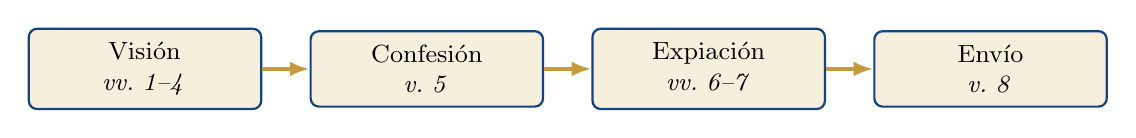
\begin{tikzpicture}[font=\small,node distance=0.6cm,
  b/.style={draw=azul,line width=0.8pt,fill=papiro,rounded corners=3pt,text width=2.6cm,align=center,inner sep=5pt}]
 \node[b] (a) {Visión\\ \emph{vv.~1--4}};
 \node[b,right=of a] (b2) {Confesión\\ \emph{v.~5}};
 \node[b,right=of b2] (c) {Expiación\\ \emph{vv.~6--7}};
 \node[b,right=of c] (d) {Envío\\ \emph{v.~8}};
 \foreach \i/\j in {a/b2,b2/c,c/d}\draw[-{Latex[length=2.5mm]},dorado,line width=1.2pt](\i)--(\j);
\end{tikzpicture}\par
{\footnotesize\color{gris}\textit{Figura 1.} Secuencia de Is 6:1--8. \textit{Nota.} Elaboración propia.}
\end{center}

%===================================================================
\section{Sin igual: “No hay santo como el \SENOR”}

La santidad es lo que hace a Dios único. Lo dice Ana, madre de Samuel, en la oración que pronuncia cuando entrega al hijo que había pedido (1~S 1:27--2:1):

\hebverso{אֵין־קָדוֹשׁ כַּיהוָה כִּי־אֵין בִּלְתֶּךָ \\ וְאֵין צוּר כֵּאלֹהֵינוּ}
\begin{verso}{1 Samuel 2:2}
No hay santo como \SENOR; Porque no hay ninguno fuera de ti, Y no hay refugio como el Dios nuestro.
\end{verso}

\begin{filologia}{1~S 2:2}
\heb{אֵין} \emph{eyn} & --- & ``no hay'': niega la existencia. Se repite tres veces en el verso. \\
\heb{כַּיהוָה} \emph{ka-Adonay} & --- & ``como el \SENOR'': la partícula \heb{כְּ} introduce la comparación que se niega. \\
\heb{בִּלְתֶּךָ} \emph{biltéja} & \heb{בלה} & ``fuera de ti'', ``excepto tú''. \\
\heb{צוּר} \emph{tsur} & \heb{צור} & ``roca''; la RVR1960 traduce ``refugio''. La roca es imagen de estabilidad y amparo (Dt 32:4). \\
\end{filologia}

El paralelismo del verso iguala dos afirmaciones: ``no hay santo como el \SENOR'' y ``no hay ninguno fuera de ti''. Ser santo y ser sin igual son, en la boca de Ana, la misma cosa. La misma idea aparece en la pregunta que canta Israel junto al mar:

\hebverso{מִי־כָמֹכָה בָּאֵלִם יְהוָה \\ מִי כָּמֹכָה נֶאְדָּר בַּקֹּדֶשׁ}
\begin{verso}{Éxodo 15:11}
¿Quién como tú, oh \SENOR, entre los dioses? ¿Quién como tú, magnífico en santidad, terrible en maravillosas hazañas, hacedor de prodigios?
\end{verso}

\begin{filologiatexto}{Éx 15:11}
\heb{מִי כָמֹכָה} (\emph{mi jamoja}), ``¿quién como tú?'', es una pregunta sin respuesta: nadie. \heb{נֶאְדָּר} (\emph{ne'dar}, raíz \heb{אדר}) significa ``majestuoso, glorioso''; \heb{בַּקֹּדֶשׁ} (\emph{baqódesh}), ``en santidad''. Dios es incomparable precisamente en su santidad.
\end{filologiatexto}

Isaías lleva la idea hasta el cosmos. Dios mismo pregunta con quién se le puede comparar, y responde señalando las estrellas:

\hebverso{וְאֶל־מִי תְדַמְּיוּנִי וְאֶשְׁוֶה יֹאמַר קָדוֹשׁ}
\begin{verso}{Isaías 40:25–26}
¿A qué, pues, me haréis semejante o me compararéis? dice el Santo. Levantad en alto vuestros ojos, y mirad quién creó estas cosas; él saca y cuenta su ejército; a todas llama por sus nombres; ninguna faltará; tal es la grandeza de su fuerza, y el poder de su dominio.
\end{verso}

\begin{filologiatexto}{Is 40:25}
\heb{דמה} (\emph{damah}) es ``asemejar, comparar''. \heb{קָדוֹשׁ} aparece aquí sin artículo, como nombre propio: ``dice Santo''. Las estrellas, que los pueblos vecinos adoraban, son el ``ejército'' que Dios cuenta y llama por nombre.
\end{filologiatexto}

Por eso la santidad hace a Dios más grande que el universo. Todo lo que existe, desde los serafines hasta las estrellas, está del lado de lo creado. Dios está del otro lado de esa línea, y nada la cruza por sí mismo. Salomón lo dijo al dedicar el templo: ``He aquí que los cielos, los cielos de los cielos, no te pueden contener'' (1~R 8:27).

\begin{center}
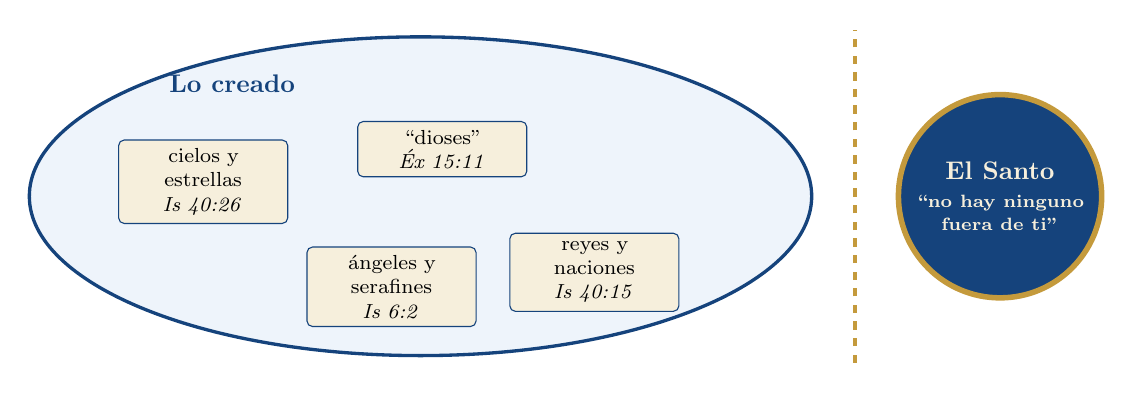
\begin{tikzpicture}[font=\small,scale=0.92,transform shape]
 \draw[azul,line width=1.2pt,fill=celeste!10] (0,0) ellipse (5.4cm and 2.2cm);
 \node[azul,font=\bfseries] at (-2.6,1.55) {Lo creado};
 \foreach \p/\t in {{(-3.0,0.2)}/{cielos y estrellas\\ \emph{Is 40:26}},{(-0.4,-1.25)}/{ángeles y serafines\\ \emph{Is 6:2}},{(2.4,-1.05)}/{reyes y naciones\\ \emph{Is 40:15}},{(0.3,0.65)}/{``dioses''\\ \emph{Éx 15:11}}}
  \node[draw=azul,fill=papiro,rounded corners=2pt,text width=2.1cm,align=center,font=\footnotesize] at \p {\t};
 \draw[dorado,line width=1.4pt,dashed] (6.0,-2.3) -- (6.0,2.3);
 \node[draw=dorado,line width=2pt,fill=azul,text=papiro,circle,minimum size=2.4cm,align=center,font=\bfseries] at (8.0,0) {El Santo\\[-1pt]{\scriptsize ``no hay ninguno}\\[-3pt]{\scriptsize fuera de ti''}};
\end{tikzpicture}\par
{\footnotesize\color{gris}\textit{Figura 2.} La santidad como distinción entre Dios y todo lo creado. \textit{Nota.} Elaboración propia.}
\end{center}

%===================================================================
\section{La palabra: la raíz \heb{קדשׁ}}

\subsection{Familia de palabras}
La raíz \heb{קדשׁ} produce el adjetivo \heb{קָדוֹשׁ} (\emph{qadosh}, ``santo''), el sustantivo \heb{קֹדֶשׁ} (\emph{qódesh}, ``santidad, lo sagrado''), el verbo \heb{קָדַשׁ} (\emph{qadash}, ``ser santo''; en las formas intensivas, ``santificar, consagrar'') y el sustantivo \heb{מִקְדָּשׁ} (\emph{miqdash}, ``santuario''). Su sentido básico es lo \destacar{apartado}: lo que pertenece al ámbito de Dios y queda separado del uso común.

Los usos son concretos antes que abstractos: hay ``tierra santa'' (\heb{אַדְמַת־קֹדֶשׁ}, Éx 3:5), un ``lugar santísimo'' (\heb{קֹדֶשׁ הַקֳּדָשִׁים}, literalmente ``santo de santos'', otro superlativo por repetición), vestiduras santas, aceite santo y un día santo. Isaías llama a Dios \heb{קְדוֹשׁ יִשְׂרָאֵל} (\emph{qedosh Yisra'el}), ``el Santo de Israel'', su título característico.

\precision{la etimología de \heb{קדשׁ} es discutida. Unos la relacionan con la idea de ``separar'' o ``cortar''; otros, con el acadio \emph{qadāšu}, ``ser puro, limpio'' (Koehler y Baumgartner, 2001). El uso bíblico une las dos ideas: lo santo está apartado y es puro. Según un conteo propio sobre la BHS y la RVR1960, Isaías usa ``el Santo de Israel'' 25 veces (31 en todo el Antiguo Testamento; véase la sección sobre el Nombre).}

\subsection{Lo santo y lo profano}
\hebverso{וּלֲהַבְדִּיל בֵּין הַקֹּדֶשׁ וּבֵין הַחֹל \\ וּבֵין הַטָּמֵא וּבֵין הַטָּהוֹר}
\begin{verso}{Levítico 10:10}
para poder discernir entre lo santo y lo profano, y entre lo inmundo y lo limpio.
\end{verso}

\begin{filologiatexto}{Lv 10:10}
\heb{הַבְדִּיל} (\emph{havdil}, raíz \heb{בדל}) es ``separar, distinguir''; es el verbo de la creación: ``separó Dios la luz de las tinieblas'' (Gn 1:4). \heb{חֹל} (\emph{jol}) es lo profano o común, lo que no está consagrado. \heb{טָמֵא} (\emph{tame}) es lo inmundo y \heb{טָהוֹר} (\emph{tahor}), lo limpio.
\end{filologiatexto}

El sacerdote debía enseñar a Israel a distinguir. Lo común no es necesariamente malo; simplemente no está apartado para Dios. Lo inmundo, en cambio, no puede acercarse a lo santo. La santidad de Dios ordena toda la vida de Israel alrededor de esa doble distinción.

\subsection{Del hebreo a Pablo}
La Septuaginta traduce casi siempre \emph{qadosh} con \grc{ἅγιος} (\emph{hágios}) y el verbo con \grc{ἁγιάζω} (\emph{hagiázō}). Pablo hereda esas palabras con su carga hebrea y añade dos sustantivos: \grc{ἁγιασμός} (\emph{hagiasmós}, ``santificación'', 1~Ts 4:3, 7; 1~Co 1:30) y \grc{ἁγιωσύνη} (\emph{hagiōsýnē}, ``santidad'' como cualidad), que en el Nuevo Testamento solo aparece en Pablo (Ro 1:4; 2~Co 7:1; 1~Ts 3:13; Bauer et~al., 2000).

\begin{center}
\begin{tikzpicture}[font=\small,node distance=0.8cm,
  b/.style={draw=azul,line width=0.8pt,fill=papiro,rounded corners=3pt,text width=3.4cm,align=center,inner sep=5pt}]
 \node[b] (h) {\textbf{Hebreo}\\ \heb{קָדוֹשׁ} \emph{qadosh}\\ \heb{קֹדֶשׁ} \emph{qódesh}};
 \node[b,right=of h] (l) {\textbf{Septuaginta}\\ \grc{ἅγιος} \emph{hágios}\\ \grc{ἁγιάζω} \emph{hagiázō}};
 \node[b,right=of l] (p) {\textbf{Pablo}\\ \grc{ἁγιασμός} \emph{hagiasmós}\\ \grc{ἁγιωσύνη} \emph{hagiōsýnē}};
 \draw[-{Latex[length=2.5mm]},dorado,line width=1.2pt](h)--(l);
 \draw[-{Latex[length=2.5mm]},dorado,line width=1.2pt](l)--(p);
\end{tikzpicture}\par
{\footnotesize\color{gris}\textit{Figura 3.} El vocabulario de la santidad del hebreo a Pablo. \textit{Nota.} Elaboración propia.}
\end{center}

%===================================================================
\section{El Nombre que revela la santidad}

En la Escritura el nombre de Dios no es una etiqueta: es la revelación de lo que él es. Moisés pidió ver la gloria y Dios respondió proclamando su Nombre (Éx 33:18--19; 34:5--7). Con la santidad la Biblia va más lejos que con cualquier otro atributo: no solo dice que Dios es santo, sino que \destacar{su nombre es ``Santo''}.

\subsection{“Cuyo nombre es el Santo”}
\hebverso{כִּי כֹה אָמַר רָם וְנִשָּׂא שֹׁכֵן עַד וְקָדוֹשׁ שְׁמוֹ \\ מָרוֹם וְקָדוֹשׁ אֶשְׁכּוֹן וְאֶת־דַּכָּא וּשְׁפַל־רוּחַ}
\begin{verso}{Isaías 57:15a}
Porque así dijo el Alto y Sublime, el que habita la eternidad, y cuyo nombre es el Santo: \ldots
\end{verso}

\begin{filologia}{Is 57:15}
\heb{קָדוֹשׁ שְׁמוֹ} \emph{qadosh shemó} & \heb{קדשׁ}, \heb{שׁם} & ``santo (es) su nombre''; la RVR1960 traduce ``cuyo nombre es el Santo''. La santidad no se agrega al Nombre: es el Nombre. La misma fórmula aparece en Sal 111:9 y en el cántico de María (Lc 1:49). \\
\heb{רָם וְנִשָּׂא} \emph{ram venissá} & \heb{רום}, \heb{נשׂא} & ``alto y sublime'': los mismos dos participios que describen el trono de Is 6:1. Isaías vuelve a la visión del texto ancla. \\
\heb{שֹׁכֵן עַד} \emph{shojen ad} & \heb{שׁכן} & ``el que habita la eternidad''. De la raíz \heb{שׁכן}, ``habitar'', viene \heb{מִשְׁכָּן} (\emph{mishkán}), el tabernáculo. \\
\heb{דַּכָּא} \emph{dakká} & \heb{דכא} & ``quebrantado, molido'' (v.~15b; el texto completo se cita en la definición): el mismo verbo de Is 53:5 (``molido por nuestros pecados''). \\
\end{filologia}

El verso completo, que se cita en la definición, une lo que parecería imposible de unir. El que se llama ``Santo'' y habita la eternidad habita también con el quebrantado y humilde de espíritu. Su nombre lo separa de todo lo creado, pero esa separación no lo aleja del humilde: lo acerca para darle vida.

\precision{de la raíz \heb{שׁכן} la tradición rabínica formó el término \emph{Shejiná}, la presencia de Dios que habita en medio de su pueblo. La palabra no aparece en la Biblia hebrea; es posterior.}

\subsection{“El Santo de Israel”}
\hebverso{אֲנִי עֲזַרְתִּיךְ נְאֻם־יְהוָה \\ וְגֹאֲלֵךְ קְדוֹשׁ יִשְׂרָאֵל}
\begin{verso}{Isaías 41:14}
No temas, gusano de Jacob, oh vosotros los pocos de Israel; yo soy tu socorro, dice \SENOR{}; el Santo de Israel es tu Redentor.
\end{verso}

\begin{filologia}{Is 41:14}
\heb{קְדוֹשׁ יִשְׂרָאֵל} \emph{qedosh Yisra'el} & \heb{קדשׁ} & ``el Santo de Israel'', en estado constructo: el Santo que se ha ligado a un pueblo. El título une las dos caras de la santidad: separado de todo, comprometido con Israel. \\
\heb{גֹּאֲלֵךְ} \emph{go'alej} & \heb{גאל} & ``tu redentor''. El \emph{go'el} es el pariente cercano que rescata la tierra o la persona de su familia (Lv 25:25; Rt 4:4--6). El Santo se presenta como pariente. \\
\heb{תּוֹלַעַת יַעֲקֹב} \emph{tola'at Ya'aqov} & \heb{תולע} & ``gusano de Jacob'': lo más pequeño y despreciable. \\
\end{filologia}

``El Santo de Israel'' es el título característico de Isaías. Según un conteo propio sobre la BHS y la RVR1960, aparece 31 veces en el Antiguo Testamento: 25 en Isaías, repartidas en todo el libro (desde 1:4 hasta 60:14), 3 en los Salmos (71:22; 78:41; 89:18 [19]), 2 en Jeremías (50:29; 51:5) y 1 en 2~Reyes (19:22, el mismo oráculo de Is 37:23). Isaías, que vio al Santo en el templo (Is 6:3), no dejó de llamarlo así.

\subsection{“Yo \SENOR{} que os santifico”}
\hebverso{וּשְׁמַרְתֶּם אֶת־חֻקֹּתַי וַעֲשִׂיתֶם אֹתָם \\ אֲנִי יְהוָה מְקַדִּשְׁכֶם}
\begin{verso}{Levítico 20:8}
Y guardad mis estatutos, y ponedlos por obra. Yo \SENOR{} que os santifico.
\end{verso}

\begin{filologiatexto}{Lv 20:8}
\heb{מְקַדִּשְׁכֶם} (\emph{meqaddishjem}) es el participio piel de \heb{קדשׁ}: ``el que os santifica'', una acción continua. La fórmula ``Yo \SENOR{} que os santifico'' acompaña al Nombre en Éx 31:13 (el día de reposo como señal) y en Lv 20:8; 21:8; 22:32. El Nombre santo es también el Nombre que hace santos.
\end{filologiatexto}

Aquí se ve la clasificación del atributo. La santidad de Dios es incomunicable en su plenitud: solo él es ``el Santo''. Pero se comunica como reflejo, porque el mismo Nombre que separa a Dios de todo santifica a su pueblo.

\subsection{El Nombre santo en Cristo, leído con Pablo}
El Nuevo Testamento da a Jesús los títulos del Santo: ``el Santo de Dios'' (\grc{ὁ ἅγιος τοῦ θεοῦ}, Mr 1:24), ``el Santo y el Justo'' (Hch 3:14) y, en boca del Resucitado, ``el Santo, el Verdadero'' (Ap 3:7). Pablo une el Nombre con la santificación del creyente:

\begin{verso}{1 Corintios 6:11}
Y esto erais algunos; mas ya habéis sido lavados, ya habéis sido santificados, ya habéis sido justificados en el nombre del Señor Jesús, y por el Espíritu de nuestro Dios.
\end{verso}

\begin{filologiatexto}{1~Co 6:11}
\grc{ἡγιάσθητε} (\emph{hēgiásthēte}) es aoristo pasivo de \grc{ἁγιάζω}: ``fuisteis santificados'', una acción ya cumplida por otro. \grc{ἐν τῷ ὀνόματι τοῦ κυρίου} (\emph{en tō onómati tou kyríou}): ``en el nombre del Señor''. Lo que Levítico atribuía al \SENOR{} que santifica (\emph{meqaddishjem}), Pablo lo atribuye al nombre del Señor Jesús.
\end{filologiatexto}

\precision{el paralelo entre Lv 20:8 y 1~Co 6:11 es lectura propia: Pablo no cita Levítico en este verso. En la literatura rabínica, una de las designaciones más frecuentes de Dios es \emph{HaQadosh Barukh Hu} (\heb{הַקָּדוֹשׁ בָּרוּךְ הוּא}), ``el Santo, bendito sea'': con ella comienza, por ejemplo, el diálogo de \emph{Shemot Rabá} 3:6 sobre el Nombre.}

\begin{center}
\small\renewcommand{\arraystretch}{1.2}
\begin{tabular}{@{}L{4.2cm}L{3.6cm}L{3.0cm}L{4.6cm}@{}}
\toprule
\textbf{Nombre o título} & \textbf{Hebreo / griego} & \textbf{Texto} & \textbf{Qué revela} \\ \midrule
``Santo es su nombre'' & \heb{קָדוֹשׁ שְׁמוֹ} & Is 57:15; Sal 111:9; Lc 1:49 & La santidad es el Nombre \\
``El Santo'' & \heb{קָדוֹשׁ} & Is 40:25 & Sin igual, sin comparación \\
``El Santo de Israel'' & \heb{קְדוֹשׁ יִשְׂרָאֵל} & Is 41:14 (31 veces) & El Santo ligado a su pueblo \\
``\SENOR{} de los ejércitos'' & \heb{יְהוָה צְבָאוֹת} & Is 6:3 & El Nombre en el trisagio \\
``\SENOR{} que os santifico'' & \heb{יְהוָה מְקַדִּשְׁכֶם} & Lv 20:8; Éx 31:13 & El Santo que hace santos \\
``El Santo de Dios'', ``el Santo y el Justo'' & \grc{ὁ ἅγιος τοῦ θεοῦ} & Mr 1:24; Hch 3:14; Ap 3:7 & El título en Jesús \\
\emph{HaQadosh Barukh Hu} & \heb{הַקָּדוֹשׁ בָּרוּךְ הוּא} & Literatura rabínica & Nombre habitual en los sabios \\ \bottomrule
\end{tabular}\par\smallskip
{\footnotesize\color{gris}\textit{Tabla.} La santidad en los nombres de Dios. \textit{Nota.} Elaboración propia; conteo propio sobre la BHS y la RVR1960.}
\end{center}

%===================================================================
\section{Definición}

\begin{tcolorbox}[colback=papiro,colframe=azul,boxrule=1pt,arc=3pt,fonttitle=\bfseries,title=La santidad de Dios]
La santidad es la perfección eterna por la cual Dios es \destacar{absolutamente distinto} de todo lo creado y \destacar{absolutamente puro} de todo mal. Es lo que lo hace único, sin igual (1~S 2:2), y lo que da a cada uno de sus atributos su carácter divino.
\end{tcolorbox}

La definición tiene dos dimensiones y una consecuencia. La primera es la \emph{majestad}: Dios es distinto de toda criatura y nada se le compara (Éx 15:11; Is 40:25). La segunda es la \emph{pureza}: Dios es limpio de todo mal. ``Muy limpio eres de ojos para ver el mal, ni puedes ver el agravio'' (Hab 1:13). La consecuencia sorprende: el Dios que está infinitamente por encima es el mismo que se acerca.

\begin{verso}{Isaías 57:15}
Porque así dijo el Alto y Sublime, el que habita la eternidad, y cuyo nombre es el Santo: Yo habito en la altura y la santidad, y con el quebrantado y humilde de espíritu, para hacer vivir el espíritu de los humildes, y para vivificar el corazón de los quebrantados.
\end{verso}

\begin{filologiatexto}{Is 57:15}
\heb{רָם וְנִשָּׂא} (\emph{ram venissá}), ``alto y sublime'', repite las palabras del trono de Is 6:1. \heb{דַּכָּא} (\emph{dakká}) es ``quebrantado, triturado''. El verso pone juntas ``la altura y la santidad'' y la morada con el humilde.
\end{filologiatexto}

\begin{center}\small\renewcommand{\arraystretch}{1.3}
\begin{tabular}{@{}L{3.6cm}L{5.4cm}L{5.4cm}@{}}
\toprule
\textbf{Clasificación} & \textbf{Ubicación} & \textbf{Comentario} \\ \midrule
Grupo & Identidad (¿quién es?) & La santidad define quién es Dios: su Nombre es ``el Santo'' (Is 57:15). \\
Tipo & Incomunicable en su plenitud; comunicable como reflejo & Nadie es santo como él (1~S 2:2), pero manda: ``Santos seréis, porque santo soy yo'' (Lv 19:2). \\
\bottomrule
\end{tabular}\end{center}

\precision{la clasificación doble (incomunicable en su plenitud, comunicable como reflejo) es una propuesta de este estudio para recoger los dos grupos de textos.}

%===================================================================
\section{La santidad que permea todos sus atributos}

La Escritura no se limita a decir que Dios es poderoso, justo, fiel o misericordioso. Dice que su brazo es \emph{santo}, que su justicia lo muestra \emph{santo}, que jura por su \emph{santidad} y que perdona porque es el \emph{Santo}. La santidad no se suma a los demás atributos: los califica a todos. Por eso el poder de Dios no es arbitrario, su celo no es egoísta y su misericordia no es complicidad con el mal.

\begin{center}
\begin{tikzpicture}[font=\small]
 \node[draw=dorado,line width=2pt,fill=azul,text=papiro,circle,minimum size=2.4cm,font=\large\bfseries,align=center] (c) at (0,0) {SANTO\\[-2pt]{\small\heb{קָדוֹשׁ}}};
 \foreach \ang/\t/\r in {90/{Nombre}/{Sal 111:9},45/{Poder}/{Is 52:10},0/{Justicia}/{Is 5:16},-45/{Fidelidad}/{Sal 89:35},-90/{Celo}/{Jos 24:19},-135/{Misericordia}/{Os 11:9},180/{Sabiduría}/{Pr 9:10},135/{Eternidad}/{Is 57:15}}{
  \node[draw=azul,fill=papiro,rounded corners=3pt,text width=2.1cm,align=center,inner sep=4pt] (n) at (\ang:3.4cm) {\textbf{\textcolor{azul}{\t}}\\ {\footnotesize\r}};
  \draw[dorado,line width=1.1pt] (c) -- (n);}
\end{tikzpicture}\par
{\footnotesize\color{gris}\textit{Figura 4.} La santidad como centro que califica a los demás atributos. \textit{Nota.} Elaboración propia.}
\end{center}

\begin{center}\small\renewcommand{\arraystretch}{1.25}
\begin{tabular}{@{}L{2.2cm}L{6.6cm}L{1.8cm}L{3.6cm}@{}}
\toprule
\textbf{Atributo} & \textbf{Texto (RVR1960)} & \textbf{Cita} & \textbf{Lo que muestra} \\ \midrule
Nombre & ``Santo y temible es su nombre.'' & Sal 111:9 & la santidad es su identidad \\
Eternidad & ``el que habita la eternidad, y cuyo nombre es el Santo'' & Is 57:15 & eterno y santo a la vez \\
Poder & ``\SENOR{} desnudó su santo brazo ante los ojos de todas las naciones'' & Is 52:10 & poder que salva, sin abuso \\
Justicia & ``el Dios Santo será santificado con justicia'' & Is 5:16 & juicio sin corrupción \\
Fidelidad & ``Una vez he jurado por mi santidad, y no mentiré a David.'' & Sal 89:35 [89:36] & jura por lo más alto que es \\
Celo & ``él es Dios santo, y Dios celoso'' & Jos 24:19 & celo sin egoísmo \\
Misericordia & ``porque Dios soy, y no hombre, el Santo en medio de ti'' & Os 11:9 & perdona \emph{porque} es santo \\
Sabiduría & ``el conocimiento del Santísimo es la inteligencia'' & Pr 9:10 & la sabiduría comienza en él \\
Verdad & ``Esto dice el Santo, el Verdadero'' & Ap 3:7 & santo y verdadero (dicho de Cristo) \\
\bottomrule
\end{tabular}\end{center}

Oseas 11:9 merece atención. Israel merecía el juicio, y Dios dice: ``No ejecutaré el ardor de mi ira, ni volveré para destruir a Efraín; porque Dios soy, y no hombre, el Santo en medio de ti''. La razón de la misericordia es la santidad: Dios no reacciona como un hombre ofendido, porque no es hombre.

\begin{filologiatexto}{Os 11:9}
\heb{כִּי אֵל אָנֹכִי וְלֹא־אִישׁ בְּקִרְבְּךָ קָדוֹשׁ}: ``porque Dios (\heb{אֵל}, \emph{El}) soy yo, y no hombre (\heb{אִישׁ}, \emph{ish}); en medio de ti, santo''. La santidad aparece aquí como alteridad: Dios es distinto del hombre incluso en su manera de perdonar.
\end{filologiatexto}

%===================================================================
\section{Teología: el Santo frente al pecado}

Si la santidad califica todos los atributos, también determina cómo se relaciona Dios con el pecado y cómo debe acercarse a él la criatura. La pregunta de Moisés después del mar abre el camino:

\begin{verso}{Éxodo 15:11}
¿Quién como tú, oh \SENOR{}, entre los dioses? ¿Quién como tú, magnífico en santidad, terrible en maravillosas hazañas, hacedor de prodigios?
\end{verso}

La pregunta no espera respuesta, porque no la hay. Solo Dios es santo en sí mismo; todo lo demás que la Escritura llama santo (la tierra de la zarza, el sábado, el altar, el pueblo) lo es porque él lo aparta para sí: ``Yo \SENOR{} que os santifico'' (Lv 20:8). La santidad de la criatura es siempre derivada; la de Dios, original. Ana lo confiesa con la misma fórmula: ``No hay santo como \SENOR{}'' (1~S 2:2).

Esa santidad no queda escondida. Se muestra en lo que Dios hace y, de modo especial, en lo que manda. Pablo, que conocía la ley desde dentro, no la culpa por el pecado del hombre: ``De manera que la ley a la verdad es santa, y el mandamiento santo, justo y bueno'' (Ro 7:12). La ley es santa porque refleja al Dios que la dio. Pero el lugar donde la santidad se ve con más claridad es la cruz: allí Dios no pasó por alto el pecado ni siquiera cuando lo cargó su propio Hijo, el que ``no escatimó ni a su propio Hijo, sino que lo entregó por todos nosotros'' (Ro 8:32). Esta lectura de la cruz como la mayor revelación de la santidad la desarrolla Pink en su exposición del atributo (Pink, 2020).

De aquí se siguen dos consecuencias que la Escritura une. La primera es que el Santo no puede ser indiferente al mal: ``Muy limpio eres de ojos para ver el mal, ni puedes ver el agravio'' (Hab 1:13; cf. Sal 5:4--5). Su rechazo del pecado no es un enojo pasajero, sino la reacción de su pureza ante lo que la contradice. La segunda es que nadie puede presentarse ante él apoyado en su propio mérito. Isaías, el profeta más recto de su generación, al ver al Santo dijo ``¡Ay de mí! que soy muerto'' (Is 6:5), y más tarde confesó por todo el pueblo: ``todas nuestras justicias como trapo de inmundicia'' (Is 64:6). Si la santidad de Dios es la medida, ninguna obra humana alcanza; por eso el carbón del altar tuvo que venir de Dios a los labios del profeta, y no al revés.

La consecuencia final es la adoración. Al Dios santo no se le trata con familiaridad descuidada: ``Dios temible en la gran congregación de los santos, y formidable sobre todos cuantos están alrededor de él'' (Sal 89:7 [89:8]). El Salmo 99 convierte esa reverencia en canto:

\begin{verso}{Salmo 99:9}
Exaltad a \SENOR{} nuestro Dios, y postraos ante su santo monte, porque \SENOR{} nuestro Dios es santo.
\end{verso}

\begin{filologiatexto}{Sal 99}
El salmo repite como estribillo ``él es santo'' (\heb{קָדוֹשׁ הוּא}, vv.~3 y 5) y cierra con ``santo es el \SENOR{} nuestro Dios'' (v.~9). La forma del salmo reproduce el trisagio: tres veces, en tres estrofas.
\end{filologiatexto}

\precision{la idea de la santidad como la ``hermosura'' de Dios, que da brillo a todos sus demás atributos, viene de Stephen Charnock (1682/1996), autor puritano al que Pink sigue de cerca. Lo que en esta sección se atribuye a Pink es paráfrasis de su exposición, no cita textual.}

%===================================================================
\section{Un encuentro en la historia de Israel: Moisés en la zarza}

Moisés lleva cuarenta años como pastor en Madián. Junto a Horeb ve una zarza que arde sin consumirse y se acerca a mirar (Éx 3:1--3). Entonces Dios lo llama por su nombre y lo detiene:

\hebverso{אַל־תִּקְרַב הֲלֹם שַׁל־נְעָלֶיךָ מֵעַל רַגְלֶיךָ \\ כִּי הַמָּקוֹם אֲשֶׁר אַתָּה עוֹמֵד עָלָיו אַדְמַת־קֹדֶשׁ הוּא}
\begin{verso}{Éxodo 3:5–6}
Y dijo: No te acerques; quita tu calzado de tus pies, porque el lugar en que tú estás, tierra santa es. Y dijo: Yo soy el Dios de tu padre, Dios de Abraham, Dios de Isaac, y Dios de Jacob. Entonces Moisés cubrió su rostro, porque tuvo miedo de mirar a Dios.
\end{verso}

\begin{filologia}{Éx 3:5}
\heb{אַל־תִּקְרַב} \emph{al-tiqrav} & \heb{קרב} & ``no te acerques''. Es la raíz de \emph{qorbán}, la ofrenda que ``se acerca'' al altar. A Dios solo se llega por el camino que él abre. \\
\heb{שַׁל} \emph{shal} & \heb{נשׁל} & ``quita'', ``desata''. Descalzarse era señal de respeto ante un superior y de reconocer que el lugar no es propio. \\
\heb{אַדְמַת־קֹדֶשׁ} \emph{admat-qódesh} & \heb{קדשׁ} & ``tierra de santidad'': el hebreo usa el sustantivo en construcción donde el español usa un adjetivo. \\
\end{filologia}

La tierra no es santa por sí misma. Era desierto común el día anterior y lo volvería a ser. La hace santa la presencia del Dios santo. La santidad, en primer lugar, no es una cualidad de las cosas sino de Dios, que santifica todo lo que toca.

\precision{según un conteo propio, Éx 3:5 es la primera aparición del sustantivo \emph{qódesh} en la Torá; conviene verificarlo en la BHS o en e-Sword. La raíz aparece antes como verbo en Gn 2:3, donde Dios ``santificó'' el séptimo día.}

Los encuentros de Moisés y de Isaías siguen el mismo patrón:

\begin{center}\small\renewcommand{\arraystretch}{1.3}
\begin{tabular}{@{}L{3.0cm}L{5.6cm}L{5.6cm}@{}}
\toprule
& \textbf{Moisés (Éx 3)} & \textbf{Isaías (Is 6)} \\ \midrule
Dios se manifiesta & fuego en la zarza (3:2) & trono, serafines ``ardientes'' y humo (6:1--4) \\
Se declara la santidad & ``tierra santa es'' (3:5) & ``Santo, santo, santo'' (6:3) \\
El hombre se cubre & ``cubrió su rostro'' (3:6) & ``¡Ay de mí!'' (6:5); los serafines cubren su rostro (6:2) \\
Dios se acerca & ``he descendido para librarlos'' (3:8) & el carbón del altar quita la culpa (6:7) \\
Envío & ``Ven, por tanto, ahora, y te enviaré'' (3:10) & ``¿A quién enviaré?''; ``Envíame a mí'' (6:8) \\
\bottomrule
\end{tabular}\end{center}

\precision{el paralelo es una lectura propia. Los dos relatos comparten la secuencia típica de los relatos de llamado profético: manifestación, objeción o temor, provisión de Dios y envío.}

En los dos casos, la santidad primero aparta al hombre y luego lo envía. El Santo no desciende para destruir, sino para librar.

%===================================================================
\section{La santidad en Cristo, leída con Pablo}

\subsection{Isaías vio su gloria}
El puente entre el trono de Isaías y Jesús lo tiende el evangelio de Juan. Después de citar Is 6:10, el evangelista afirma:

\begin{verso}{Juan 12:41}
Isaías dijo esto cuando vio su gloria, y habló acerca de él.
\end{verso}

La gloria que llenaba el templo era la gloria de Cristo. Pablo llega al mismo lugar por otro camino. En 2~Corintios 3 compara el rostro de Moisés, que brillaba después de hablar con Dios (Éx 34:29--35), con la gloria del nuevo pacto, y concluye:

\begin{verso}{2 Corintios 4:6}
Porque Dios, que mandó que de las tinieblas resplandeciese la luz, es el que resplandeció en nuestros corazones, para iluminación del conocimiento de la gloria de Dios en la faz de Jesucristo.
\end{verso}

\begin{filologiatexto}{2~Co 4:6}
\grc{δόξα} (\emph{dóxa}) es la palabra con que la Septuaginta traduce \heb{כָּבוֹד}. \grc{ἐν προσώπῳ Ἰησοῦ Χριστοῦ} (\emph{en prosōpō Iēsoû Christoû}): ``en el rostro de Jesucristo''. El \emph{kavod} que llena la tierra en Is 6:3 tiene ahora un rostro humano.
\end{filologiatexto}

\precision{el puente explícito entre Is 6 y Cristo es de Juan, no de Pablo. En 2~Co 4:6 el eco directo es Gn 1:3 (``sea la luz''); la relación con la gloria de Is 6 es un eco posible dentro del tema de la gloria (Hays, 1989).}

\subsection{“Según el Espíritu de santidad”}
Pablo presenta su evangelio con una fórmula de sabor hebreo:

\begin{verso}{Romanos 1:4}
que fue declarado Hijo de Dios con poder, según el Espíritu de santidad, por la resurrección de entre los muertos.
\end{verso}

\begin{filologiatexto}{Ro 1:4}
\grc{κατὰ πνεῦμα ἁγιωσύνης} (\emph{katà pneûma hagiōsýnēs}), ``según el espíritu de santidad''. Es un hebraísmo: reproduce la construcción de \heb{רוּחַ קָדְשְׁךָ} (\emph{rúaj qodshéja}, ``tu santo espíritu'', literalmente ``espíritu de tu santidad'', Sal 51:11 [51:13]; Is 63:10--11). \grc{ἁγιωσύνη} es un sustantivo de cualidad que en el Nuevo Testamento solo usa Pablo.
\end{filologiatexto}

Pablo, judío formado en las Escrituras de Israel, usa una expresión de los salmos para decir quién es Jesús: el Mesías resucitado pertenece a la esfera de la santidad de Dios.

\precision{se discute si ``Espíritu de santidad'' designa al Espíritu Santo o la naturaleza espiritual de Cristo en contraste con ``según la carne'' (v.~3). Moo (1996) se inclina por el Espíritu Santo; Dunn (1998) subraya el contraste entre las dos esferas de la existencia del Hijo.}

\subsection{El carbón del altar y la cruz}
En Is 6:7 el pecado de Isaías ``es expiado'' (\heb{תְּכֻפָּר}) con un carbón tomado del altar. Pablo describe la cruz con el vocabulario del mismo altar:

\begin{verso}{Romanos 3:23–26}
por cuanto todos pecaron, y están destituidos de la gloria de Dios, siendo justificados gratuitamente por su gracia, mediante la redención que es en Cristo Jesús, a quien Dios puso como propiciación por medio de la fe en su sangre, para manifestar su justicia, a causa de haber pasado por alto, en su paciencia, los pecados pasados, con la mira de manifestar en este tiempo su justicia, a fin de que él sea el justo, y el que justifica al que es de la fe de Jesús.
\end{verso}

\begin{filologiatexto}{Ro 3:25}
\grc{ἱλαστήριον} (\emph{hilastērion}), ``propiciación'' o ``propiciatorio'', es la palabra con que la Septuaginta traduce \heb{כַּפֹּרֶת} (\emph{kapporet}), la tapa del arca donde se rociaba la sangre en el Día de la Expiación (Éx 25:17; Lv 16:14--15). \emph{Kapporet} y \emph{tekuppar} (Is 6:7) comparten la raíz \heb{כפר}. Notar también ``destituidos de la gloria'' (\grc{δόξα}, v.~23): lo que el pecador pierde es justamente el \emph{kavod} que llena la tierra en Is 6:3.
\end{filologiatexto}

\begin{center}
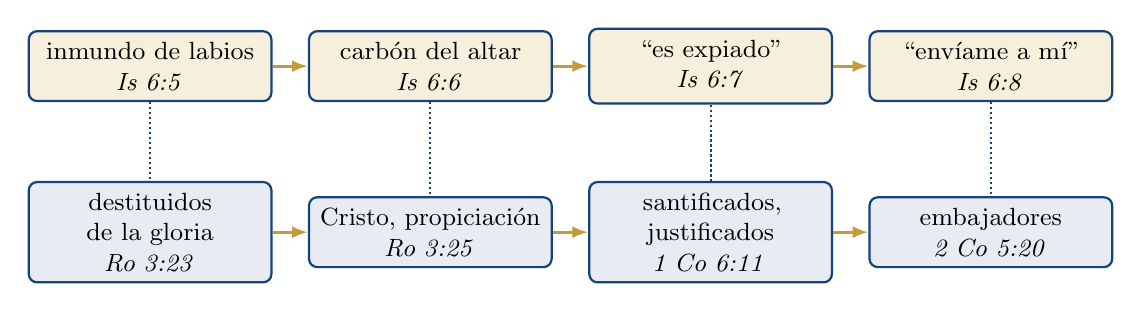
\begin{tikzpicture}[font=\small,node distance=0.45cm,
  b/.style={draw=azul,line width=0.8pt,fill=papiro,rounded corners=3pt,text width=2.8cm,align=center,inner sep=4pt}]
 \node[b] (i1) {inmundo de labios\\ \emph{Is 6:5}};
 \node[b,right=of i1] (i2) {carbón del altar\\ \emph{Is 6:6}};
 \node[b,right=of i2] (i3) {``es expiado''\\ \emph{Is 6:7}};
 \node[b,right=of i3] (i4) {``envíame a mí''\\ \emph{Is 6:8}};
 \node[b,below=1.0cm of i1,fill=azul!10] (p1) {destituidos de la gloria\\ \emph{Ro 3:23}};
 \node[b,right=of p1,fill=azul!10] (p2) {Cristo, propiciación\\ \emph{Ro 3:25}};
 \node[b,right=of p2,fill=azul!10] (p3) {santificados, justificados\\ \emph{1~Co 6:11}};
 \node[b,right=of p3,fill=azul!10] (p4) {embajadores\\ \emph{2~Co 5:20}};
 \foreach \a/\b in {i1/i2,i2/i3,i3/i4,p1/p2,p2/p3,p3/p4}\draw[-{Latex[length=2mm]},dorado,line width=1pt](\a)--(\b);
 \foreach \n in {1,2,3,4}\draw[densely dotted,azul,line width=0.8pt](i\n)--(p\n);
\end{tikzpicture}\par
{\footnotesize\color{gris}\textit{Figura 5.} La secuencia de Isaías 6 y su correspondencia en Pablo. \textit{Nota.} Elaboración propia.}
\end{center}

En la cruz se resuelve la tensión que Isaías sintió en el templo. La santidad de Dios no puede pasar por alto el pecado; si lo hiciera, dejaría de ser justo. En Cristo, Dios es ``el justo, y el que justifica'': la santidad se satisface y el pecador es limpiado.

\precision{la correspondencia entre el carbón de Is 6 y la cruz es tipológica. Pablo no cita Is 6 en Romanos 3; el vínculo es la raíz \heb{כפר} y el tema común del altar y la expiación.}

\subsection{Cristo, nuestra santificación}
Para Pablo la santidad del creyente no comienza como logro, sino como don:

\begin{verso}{1 Corintios 1:30–31}
Mas por él estáis vosotros en Cristo Jesús, el cual nos ha sido hecho por Dios sabiduría, justificación, santificación y redención, para que, como está escrito: El que se gloría, gloríese en el Señor.
\end{verso}

\begin{filologiatexto}{1~Co 1:30}
\grc{ἁγιασμός} (\emph{hagiasmós}): ``santificación'', tanto el estado de estar apartado para Dios como el proceso de vivir de acuerdo con ello (Bauer et~al., 2000). El v.~31 cita Jer 9:24, el versículo que une toda esta obra: gloriarse en conocer al Señor.
\end{filologiatexto}

\begin{verso}{1 Corintios 6:11}
Y esto erais algunos; mas ya habéis sido lavados, ya habéis sido santificados, ya habéis sido justificados en el nombre del Señor Jesús, y por el Espíritu de nuestro Dios.
\end{verso}

\begin{filologiatexto}{1~Co 6:11}
\grc{ἡγιάσθητε} (\emph{hēgiásthēte}), ``fuisteis santificados'', está en aoristo pasivo: un hecho ya cumplido y realizado por Dios. La santificación aparece aquí junto al lavamiento y la justificación como obra pasada.
\end{filologiatexto}

Lo que Isaías recibió en los labios, el creyente lo recibe en Cristo. Por eso Pablo puede llamar ``santos'' a los corintios (1~Co 1:2) al mismo tiempo que corrige sus pecados: son santos porque pertenecen al Santo, y deben llegar a ser lo que ya son. La misma idea aparece en Colosenses:

\begin{verso}{Colosenses 1:22}
en su cuerpo de carne, por medio de la muerte, para presentaros santos y sin mancha e irreprensibles delante de él.
\end{verso}

\precision{la autoría paulina de Colosenses es discutida. La enseñanza de Col 1:22 tiene respaldo en cartas indiscutidas: 1~Co 6:11 y 1~Ts 3:13.}

\subsection{La plenitud santa habita en Cristo}
La tesis de esta obra encuentra aquí su lugar: ``en él habita corporalmente toda la plenitud de la Deidad'' (Col 2:9). La santidad que los serafines proclaman está entera en Cristo, a quien Pedro llama ``el Santo y el Justo'' (Hch 3:14). En él, el Dios que Isaías no podía mirar sin decir ``¡Ay de mí!'' se deja ver, y el fuego que quema se convierte en perdón.

%===================================================================
\section{Aplicación: vivir ante el Dios santo}

\hebverso{קְדֹשִׁים תִּהְיוּ כִּי קָדוֹשׁ אֲנִי יְהוָה אֱלֹהֵיכֶם}
\begin{verso}{Levítico 19:2}
Habla a toda la congregación de los hijos de Israel, y diles: Santos seréis, porque santo soy yo \SENOR{} vuestro Dios.
\end{verso}

\begin{filologiatexto}{Lv 19:2}
\heb{תִּהְיוּ} (\emph{tihyú}), ``seréis'', es a la vez mandato y promesa. \heb{כִּי} (\emph{ki}), ``porque'', da el fundamento: la santidad de Israel deriva de la de Dios. Pedro cita este verso en 1~P 1:16.
\end{filologiatexto}

La santidad de Dios no es solo una doctrina para entender; es una realidad ante la cual se vive. El texto ancla y los demás pasajes sugieren cinco respuestas:

\begin{enumerate}
\item \textbf{Adorar con reverencia.} Moisés se quitó el calzado y los serafines se cubren el rostro (Éx 3:5; Is 6:2). La adoración no es un trato casual con Dios. ¿Qué ``tierra santa'' pisamos cada domingo sin darnos cuenta?
\item \textbf{Confesar.} Ante el Santo, Isaías no se comparó con sus vecinos: se vio a sí mismo (Is 6:5). La santidad de Dios es la única medida verdadera de nuestra condición.
\item \textbf{Recibir la santidad como don.} El carbón vino del altar, no de Isaías. Cristo nos ha sido hecho santificación (1~Co 1:30; 6:11). La vida santa empieza recibiendo, no produciendo.
\item \textbf{Vivir apartados.} ``Pues no nos ha llamado Dios a inmundicia, sino a santificación'' (1~Ts 4:7). Esto incluye el cuerpo, que Pablo pide presentar ``en sacrificio vivo, santo, agradable a Dios'' (Ro 12:1).
\item \textbf{Responder al envío.} El que ha sido limpiado escucha la pregunta ``¿A quién enviaré?'' y responde ``Heme aquí'' (Is 6:8). Pablo lo dice así: ``somos embajadores en nombre de Cristo'' (2~Co 5:20).
\end{enumerate}

\begin{verso}{1 Pedro 1:15–16}
sino, como aquel que os llamó es santo, sed también vosotros santos en toda vuestra manera de vivir; porque escrito está: Sed santos, porque yo soy santo.
\end{verso}

%===================================================================
\section{Síntesis}

\begin{tcolorbox}[colback=papiro,colframe=azul,boxrule=1pt,arc=3pt]
Dios es santo: absolutamente distinto de todo lo creado y puro de todo mal. ``No hay santo como el \SENOR; porque no hay ninguno fuera de ti'' (1~S 2:2). Por eso el cielo no canta ``eterno'' ni ``poderoso'' tres veces, sino ``Santo, santo, santo'' (Is 6:3; Ap 4:8). Su santidad califica cada atributo: su brazo es santo, su justicia lo muestra santo, jura por su santidad y perdona porque es ``Dios y no hombre'' (Os 11:9). El trono que vio Isaías es el de Cristo (Jn 12:41); la gloria de Dios brilla en su rostro (2~Co 4:6); en él habita toda la plenitud (Col 2:9), y él nos ha sido hecho santificación (1~Co 1:30).
\end{tcolorbox}

\begin{center}\small\renewcommand{\arraystretch}{1.3}
\begin{tabular}{@{}L{3.0cm}L{11.4cm}@{}}
\toprule
\textbf{Mirada} & \textbf{Aporte al atributo} \\ \midrule
Hebrea & \emph{qadosh}: lo apartado; la triple aclamación; la pregunta ``¿quién como tú?''; la tierra santa de la zarza; la santidad como alteridad que perdona (Os 11:9). \\
Teológica & Solo Dios es santo en sí mismo; su santidad se ve en la ley y en la cruz; rechaza el mal; nadie se acerca por mérito propio; pide reverencia. \\
Paulina & El Mesías declarado Hijo ``según el Espíritu de santidad''; la gloria del Santo en el rostro de Cristo; la expiación en la cruz; Cristo, nuestra santificación. \\
\bottomrule
\end{tabular}\end{center}

%===================================================================
\section*{Glosario del capítulo}
\begin{description}\setlength{\itemsep}{2pt}
\item[\emph{Adonay}] (\heb{אֲדֹנָי}). ``Señor''. Título de soberanía; también la lectura judía del tetragrama.
\item[\emph{Hagiasmós}] (\grc{ἁγιασμός}). Santificación: estado y proceso de ser apartado para Dios.
\item[\emph{Hagiōsýnē}] (\grc{ἁγιωσύνη}). Santidad como cualidad. En el Nuevo Testamento, solo en Pablo.
\item[\emph{Hilastērion}] (\grc{ἱλαστήριον}). Propiciatorio o propiciación (Ro 3:25); en la Septuaginta, la tapa del arca.
\item[\emph{Jol}] (\heb{חֹל}). Lo profano o común; lo que no está consagrado.
\item[\emph{Kapporet}] (\heb{כַּפֹּרֶת}). Tapa del arca del pacto, el propiciatorio.
\item[\emph{Kavod}] (\heb{כָּבוֹד}). Gloria; de una raíz que significa ``ser pesado''.
\item[\emph{Kipper}] (\heb{כִּפֶּר}). Expiar, cubrir la culpa.
\item[\emph{Qadosh}] (\heb{קָדוֹשׁ}). Santo, apartado para Dios.
\item[\emph{Qódesh}] (\heb{קֹדֶשׁ}). Santidad; lo sagrado.
\item[\emph{Serafim}] (\heb{שְׂרָפִים}). ``Los ardientes'', seres celestiales de Is 6:2.
\item[Tetragrama] (\heb{יהוה}). El nombre propio de Dios; en esta obra, \SENOR.
\item[Trisagio] La triple aclamación ``Santo, santo, santo'' (Is 6:3; Ap 4:8).
\item[\emph{Tseva'ot}] (\heb{צְבָאוֹת}). ``Ejércitos''; las huestes del cielo.
\item[\emph{Tsur}] (\heb{צוּר}). Roca; imagen de estabilidad y amparo (1~S 2:2).
\end{description}


% \chapter{...}\input{capitulos/05_eterno}  ...
% ===== Parte III. Relación (Sabiduría · Verdadero · Misericordioso · Fiel · Celo · Ira santa · Bondad · Paciencia · Gracia) =====
\part{Relación}
% \chapter{...}% Capítulo: La multiforme sabiduría de Dios (generado desde ../12_Sabiduria/12_Sabiduria_capitulo.tex)
% Texto ancla: Proverbios 8:22–31 (con Pr 3:19–20). Clasificación: Relación; incomunicable en su plenitud, comunicable como don.

\section{Introducción: no se alabe el sabio}

El verso que une esta obra comienza hablando de la sabiduría. Antes de decir en qué debe gloriarse el ser humano, Jeremías dice en qué no:

\hebverso{כֹּה אָמַר יְהוָה אַל־יִתְהַלֵּל חָכָם בְּחָכְמָתוֹ\\ הַשְׂכֵּל וְיָדֹעַ אוֹתִי כִּי אֲנִי יְהוָה}
\begin{verso}{Jeremías 9:23–24 [9:22–23]}
Así dijo \SENOR: No se alabe el sabio en su sabiduría, ni en su valentía se alabe el valiente, ni el rico se alabe en sus riquezas. Mas alábese en esto el que se hubiere de alabar: en entenderme y conocerme, que yo soy \SENOR, que hago misericordia, juicio y justicia en la tierra; porque estas cosas quiero, dice \SENOR.
\end{verso}

La primera gloria que el profeta descarta es la del \emph{jajam} en su \emph{jojmá}, el sabio en su sabiduría. La única gloria legítima es \heb{הַשְׂכֵּל וְיָדֹעַ אוֹתִי} (\emph{haskel veyadoa otí}), ``entender y conocer'' a Dios. El orden no es casual: la sabiduría humana es la primera que debe rendirse, porque es la que con más facilidad se cree autosuficiente. Este capítulo estudia la sabiduría que no se rinde ante nadie, porque no la recibió de nadie: la de Dios.

El libro de Job formula la pregunta de fondo. El capítulo 28 describe al minero que perfora la roca, desvía los ríos y saca a la luz el oro y las piedras preciosas, pero no encuentra la sabiduría:

\begin{verso}{Job 28:12}
Mas ¿dónde se hallará la sabiduría? ¿Dónde está el lugar de la inteligencia?
\end{verso}

La respuesta llega al final del poema: solo Dios conoce su lugar, porque la usó al crear.

\begin{verso}{Job 28:23–28}
Dios entiende el camino de ella, y conoce su lugar. Porque él mira hasta los fines de la tierra, y ve cuanto hay bajo los cielos. Al dar peso al viento, y poner las aguas por medida; cuando él dio ley a la lluvia, y camino al relámpago de los truenos, entonces la veía él, y la manifestaba; la preparó y la descubrió también. Y dijo al hombre: He aquí que el temor del Señor es la sabiduría, y el apartarse del mal, la inteligencia.
\end{verso}

Dios ``dio peso al viento'' y puso ``las aguas por medida'': la sabiduría aparece como la destreza con que el Creador calibra el mundo. Al ser humano le toca la sabiduría bajo otra forma, como \emph{temor del Señor}. No la posee como Dios; la recibe en una relación.

Por eso esta serie coloca la sabiduría entre los atributos de la \emph{relación}, los que responden a la pregunta ¿cómo se revela Dios? Como todos los atributos, es una perfección eterna de Dios. Es \emph{incomunicable} en su plenitud, porque solo Dios es ``el único y sabio Dios'' (Ro 16:27) y nadie le enseñó ni lo aconsejó (Is 40:13--14); y es \emph{comunicable} como don, porque ``\SENOR{} da la sabiduría'' (Pr 2:6) y la da ``a todos abundantemente y sin reproche'' (Stg 1:5).

\begin{center}\small\renewcommand{\arraystretch}{1.25}
\begin{tabular}{@{}L{3.4cm}L{5.4cm}L{5.6cm}@{}}
\toprule
\textbf{Mirada} & \textbf{Pregunta} & \textbf{Textos centrales} \\ \midrule
Hebrea & ¿Cómo dice Israel la sabiduría de Dios? & Pr 3:19--20; 8:22--31; Sal 104:24; Jer 10:12; Gn 50:20 \\
Judía & ¿Cómo la leen los sabios de Israel? & \emph{Bereshit Rabá} 1:1; Rashi a Éx 31:3; \emph{Berajot} 58a, 60b; 1QS III \\
Pink & ¿Qué afirma la Escritura y qué exige? & Pink (2020, caps. 2 y 8) \\
Paulina & ¿Qué lugar tiene en Cristo? & 1~Co 1:18--31; 2:7--8; Ro 11:33--36; Ef 1:10; 3:10; Col 1:15--17; 2:3 \\
\bottomrule
\end{tabular}\end{center}

%===================================================================
\section{Texto ancla: Proverbios 8:22--31}

\subsection{La Sabiduría junto al Creador}

En Proverbios 8 la Sabiduría habla en primera persona. Después de llamar a los hombres en las puertas de la ciudad (8:1--21), cuenta su origen: estaba con Dios antes de que existiera el mundo, y estaba presente cuando lo hizo.

\hebverso{יְהוָה קָנָנִי רֵאשִׁית דַּרְכּוֹ קֶדֶם מִפְעָלָיו מֵאָז\\ וָאֶהְיֶה אֶצְלוֹ אָמוֹן וָאֶהְיֶה שַׁעֲשֻׁעִים יוֹם יוֹם}
\begin{verso}{Proverbios 8:22–31}
\SENOR{} me poseía en el principio, ya de antiguo, antes de sus obras. Eternamente tuve el principado, desde el principio, antes de la tierra. Antes de los abismos fui engendrada; antes que fuesen las fuentes de las muchas aguas. Antes que los montes fuesen formados, antes de los collados, ya había sido yo engendrada; no había aún hecho la tierra, ni los campos, ni el principio del polvo del mundo. Cuando formaba los cielos, allí estaba yo; cuando trazaba el círculo sobre la faz del abismo; cuando afirmaba los cielos arriba, cuando afirmaba las fuentes del abismo; cuando ponía al mar su estatuto, para que las aguas no traspasasen su mandamiento; cuando establecía los fundamentos de la tierra, con él estaba yo ordenándolo todo, y era su delicia de día en día, teniendo solaz delante de él en todo tiempo. Me regocijo en la parte habitable de su tierra; y mis delicias son con los hijos de los hombres.
\end{verso}

\begin{filologia}{Pr 8:22--31}
\heb{קָנָנִי} \emph{qanani} (v. 22) & \heb{קנה} & ``me adquirió, me poseyó''. La LXX traduce \grc{ἔκτισέν με}, ``me creó'', lectura que pesó en los debates cristológicos de los siglos IV y V. \\
\heb{רֵאשִׁית דַּרְכּוֹ} (v. 22) & \heb{ראשׁ} & ``principio de su camino'': la misma palabra con que empieza Gn 1:1 (\heb{בְּרֵאשִׁית}). \\
\heb{נִסַּכְתִּי} \emph{nissajti} (v. 23) & \heb{נסך} & ``fui establecida'' (RVR1960: ``tuve el principado''). \\
\heb{חוּג} \emph{jug} (v. 27) & \heb{חוג} & ``círculo, bóveda'': Dios traza con compás el horizonte sobre el abismo. \\
\heb{חֻקּוֹ} \emph{juqqó} (v. 29) & \heb{חקק} & ``su estatuto'', de ``grabar'': el mar tiene un límite grabado. \\
\heb{אָמוֹן} \emph{amón} (v. 30) & \heb{אמן} & ``artesano, maestro de obras'' (cf. \heb{אָמָּן} \emph{ommán}, ``artista'', Cnt 7:1 [7:2]); otros vocalizan \heb{אָמוּן}, ``niño criado''. RVR1960: ``ordenándolo todo''; LXX: \grc{ἁρμόζουσα}, ``ajustando, armonizando''. \\
\heb{מְשַׂחֶקֶת} \emph{mesajéqet} (vv. 30--31) & \heb{שׂחק} & ``jugando, regocijándose'': la creación es obra de deleite, no de esfuerzo. \\
\end{filologia}

El texto no presenta a una Sabiduría que observa desde afuera. La presenta \emph{junto} a Dios (\heb{אֶצְלוֹ}) mientras traza el horizonte, fija el límite del mar y pone los cimientos de la tierra. El término clave es \emph{amón}. Leído como ``artesano'', describe a la Sabiduría como el maestro de obras del cosmos; leído como ``niño criado'', la describe como la hija en que Dios se deleita. La RVR1960 tradujo el sentido con una frase: ``con él estaba yo ordenándolo todo''. La Septuaginta, siglos antes, había escogido \grc{ἁρμόζουσα}: la que ajusta y pone en armonía las partes. Las dos versiones coinciden en lo esencial: la sabiduría es lo que hace que el mundo no sea un amontonamiento de cosas, sino una obra ordenada.

\precision{la Sabiduría de Proverbios 8 es una personificación poética de un atributo de Dios. Leerla como figura de Cristo es una lectura tipológica del Nuevo Testamento y de la tradición cristiana (ver sección~\ref{sec:cristo}); el texto de Proverbios no la identifica con una persona divina.}

\subsection{Con sabiduría fundó la tierra}

Proverbios 3 dice lo mismo en forma de sentencia, y Jeremías lo repite casi con las mismas palabras:

\hebverso{יְהוָה בְּחָכְמָה יָסַד־אָרֶץ כּוֹנֵן שָׁמַיִם בִּתְבוּנָה\\ בְּדַעְתּוֹ תְּהוֹמוֹת נִבְקָעוּ וּשְׁחָקִים יִרְעֲפוּ־טָל}
\begin{verso}{Proverbios 3:19–20}
\SENOR{} con sabiduría fundó la tierra; afirmó los cielos con inteligencia. Con su ciencia los abismos fueron divididos, y destilan rocío los cielos.
\end{verso}

\hebverso{עֹשֵׂה אֶרֶץ בְּכֹחוֹ מֵכִין תֵּבֵל בְּחָכְמָתוֹ וּבִתְבוּנָתוֹ נָטָה שָׁמָיִם}
\begin{verso}{Jeremías 10:12}
El que hizo la tierra con su poder, el que puso en orden el mundo con su saber, y extendió los cielos con su sabiduría.
\end{verso}

\begin{filologia}{Pr 3:19--20 y Jer 10:12}
\heb{בְּחָכְמָה} \emph{bejojmá} & \heb{חכם} & ``con sabiduría'': el instrumento con que Dios ``fundó'' (\heb{יָסַד}) la tierra. \\
\heb{בִּתְבוּנָה} \emph{bitvuná} & \heb{בין} & ``con inteligencia, discernimiento'': la capacidad de distinguir y relacionar. \\
\heb{בְּדַעְתּוֹ} \emph{beda'tó} & \heb{ידע} & ``con su conocimiento'' dividió los abismos. \\
\heb{מֵכִין} \emph{mejín} & \heb{כון} & ``establece, deja a punto'' (RVR1960: ``puso en orden''). En Jer 10:12 la RVR1960 vierte \emph{jojmá} como ``saber'' y \emph{tevuná} como ``sabiduría''. \\
\end{filologia}

Sabiduría, inteligencia y conocimiento forman una tríada. La misma tríada vuelve en Éxodo 31:3, cuando Dios llena a Bezalel ``en sabiduría y en inteligencia, en ciencia y en todo arte'' para construir el tabernáculo. La destreza con que Dios hizo el cosmos es la que da al artesano que construye su casa. Jeremías, además, une la sabiduría al poder (\heb{בְּכֹחוֹ}): en Dios la capacidad de hacer y el saber cómo hacerlo no se separan (Job 12:13).

%===================================================================
\section{La palabra}

\subsection{La raíz \heb{ח־כ־ם}}

\emph{Jojmá} (\heb{חָכְמָה}) proviene de la raíz \heb{ח־כ־ם} (\emph{j-k-m}; Strong H2449--H2451). En hebreo bíblico esta raíz no habla de ideas abstractas, sino de habilidad experta, de destreza para hacer algo correctamente, de capacidad de producir un resultado bien hecho. Por eso un artesano, un gobernante o un justo pueden tener \emph{jojmá}. La palabra siempre implica capacidad eficaz con propósito correcto: saber hacer, y hacerlo bien (Koehler y Baumgartner, 2001). En el arameo de Daniel la palabra es la misma (\heb{חָכְמְתָא}, Dn 2:20--23), y la Septuaginta y el Nuevo Testamento la traducen \grc{σοφία} (\emph{sophía}).

\begin{center}\small\renewcommand{\arraystretch}{1.25}
\begin{tabular}{@{}L{2.4cm}L{2.3cm}L{5.6cm}L{4.1cm}@{}}
\toprule
\textbf{Ámbito} & \textbf{Ejemplo} & \textbf{Descripción} & \textbf{Texto} \\ \midrule
Destreza, técnica & Bezalel & hacer correctamente una obra (arte, oficio) bajo dirección divina & Éx 31:3 \\
Gobierno, juicio & Salomón & discernimiento para gobernar y juzgar con justicia & 1~R 3:9, 28 \\
Consejo, dirección & Jetro & ver un problema y dar una solución sabia y ordenada & Éx 18:17--21 \\
Vida justa & el justo (\emph{tsaddiq}) & conducta recta que refleja sabiduría en la vida diaria & Pr 20:7 \\
Hablar sabio & el justo & expresar sabiduría con la boca: enseñanza, consejo & Sal 37:30 \\
Consejo colectivo & los consejeros & seguridad y dirección por muchos consejos & Pr 11:14; 20:18 \\
\bottomrule
\end{tabular}\end{center}

\begin{verso}{Éxodo 31:3–4}
y lo he llenado del Espíritu de Dios, en sabiduría y en inteligencia, en ciencia y en todo arte, para inventar diseños, para trabajar en oro, en plata y en bronce.
\end{verso}

\begin{filologia}{Éx 31:3--4, 1~R 3:9 y Sal 37:30}
\heb{לַחְשֹׁב מַחֲשָׁבֹת} \emph{lajshov majashavot} & \heb{חשׁב} & ``para diseñar diseños'' (RVR1960: ``para inventar diseños''). La sabiduría de Bezalel se expresa en planos. \\
\heb{לֵב שֹׁמֵעַ} \emph{lev shoméa} & \heb{שׁמע} & ``corazón que escucha'' (RVR1960: ``corazón entendido''): lo que pide Salomón para juzgar (1~R 3:9). \\
\heb{יֶהְגֶּה חָכְמָה} \emph{yehgé jojmá} & \heb{הגה} & ``medita, musita sabiduría'': la boca del justo la repite en voz baja (Sal 37:30). \\
\end{filologia}

\subsection{“Sabiduría” en la Reina-Valera 1960}

El material de estudio de esta serie cuenta 226 apariciones de ``sabiduría''. Un conteo propio en la RVR1960, sin los títulos de sección que agregan los editores, da 245 apariciones de ``sabiduría'' o ``sabidurías'' en 233 versículos: 195 en el Antiguo Testamento y 50 en el Nuevo. Si se incluyen los títulos de sección, la cifra sube a 262. La tabla muestra qué palabras del original hay detrás.

\begin{center}\small\renewcommand{\arraystretch}{1.2}
\begin{tabular}{@{}L{5.6cm}L{5.2cm}r@{}}
\toprule
\textbf{Término original} & \textbf{Sentido} & \textbf{Veces} \\ \midrule
\heb{חָכְמָה} \emph{jojmá} (hebreo y arameo) & destreza sabia & 161 \\
\heb{דַּעַת} \emph{da'at}, \heb{דֵּעָה} \emph{de'á} & conocimiento & 24 \\
\heb{שֵׂכֶל} \emph{sékel}, \heb{הִשְׂכִּיל} \emph{hiskil} & perspicacia, éxito & 4 \\
\heb{תּוּשִׁיָּה} \emph{tushiyá} & sabiduría eficaz & 3 \\
\heb{בִּינָה} \emph{biná} & discernimiento & 1 \\
\heb{כֹּחַ לֵב} \emph{kóaj lev} (Job 36:5) & ``fuerza de corazón'' & 1 \\
sin término equivalente (Job 40:2) & --- & 1 \\
\grc{σοφία} \emph{sophía} & sabiduría & 50 \\
\bottomrule
\end{tabular}\end{center}

\precision{conteo propio con la RVR1960 y la BHS con números Strong; los casos sin etiqueta Strong se asignaron por la raíz del verso hebreo. Conviene verificarlo en e-Sword: la diferencia con la cifra de 226 puede venir de contar versículos en lugar de apariciones, o de otra edición.}

\subsection{La familia de la sabiduría}

La sabiduría tiene parientes en hebreo. Job 12:13 los reúne: ``Con Dios está la sabiduría y el poder; suyo es el consejo y la inteligencia'' (\heb{עִמּוֹ חָכְמָה וּגְבוּרָה לוֹ עֵצָה וּתְבוּנָה}).

\begin{center}\small\renewcommand{\arraystretch}{1.25}
\begin{tabular}{@{}L{3.0cm}L{1.4cm}L{6.0cm}L{4.0cm}@{}}
\toprule
\textbf{Término} & \textbf{Raíz} & \textbf{Imagen y sentido} & \textbf{Textos} \\ \midrule
\heb{חָכְמָה} \emph{jojmá} & \heb{חכם} & destreza para hacer bien las cosas; el ``arte'' de vivir y de obrar & Pr 3:19; Sal 104:24 \\
\heb{תְּבוּנָה} \emph{tevuná}, \heb{בִּינָה} \emph{biná} & \heb{בין} & de \heb{בֵּין}, ``entre'': distinguir una cosa de otra & Pr 3:19; Is 40:28; 1~R 3:9 \\
\heb{דַּעַת} \emph{da'at} & \heb{ידע} & conocimiento por experiencia y trato personal & Pr 3:20; Sal 19:2 [19:3] \\
\heb{עֵצָה} \emph{etsá} & \heb{יעץ} & consejo, plan, designio & Job 12:13; Is 28:29 \\
\heb{תּוּשִׁיָּה} \emph{tushiyá} & discutida & sabiduría que da resultado; éxito sólido & Is 28:29; Pr 2:7 \\
\heb{מַחֲשָׁבָה} \emph{majashavá} & \heb{חשׁב} & ``diseño, plan'' (Bezalel) y ``pensamiento'' de Dios & Éx 31:4; Is 55:8 \\
\bottomrule
\end{tabular}\end{center}

\begin{verso}{Isaías 28:29}
También esto salió de \SENOR{} de los ejércitos, para hacer maravilloso el consejo y engrandecer la sabiduría.
\end{verso}

Isaías 28:23--29 es una parábola del labrador: sabe cuándo arar, qué semilla poner en cada surco y con qué instrumento trillar cada grano. Esa destreza, dice el profeta, ``salió de \SENOR''. La palabra traducida ``sabiduría'' es \heb{תּוּשִׁיָּה} (\emph{tushiyá}): la sabiduría que funciona, que produce el resultado buscado.

\subsection{Del hebreo a Pablo}

La Septuaginta tradujo \emph{jojmá} por \grc{σοφία}: ``Dios con la sabiduría fundó la tierra'' (\grc{ὁ θεὸς τῇ σοφίᾳ ἐθεμελίωσεν τὴν γῆν}, Pr 3:19 LXX). Pablo, formado en las Escrituras de Israel, usa la misma palabra para hablar de Cristo crucificado:

\begin{verso}{1 Corintios 1:22–24}
Porque los judíos piden señales, y los griegos buscan sabiduría; pero nosotros predicamos a Cristo crucificado, para los judíos ciertamente tropezadero, y para los gentiles locura; mas para los llamados, así judíos como griegos, Cristo poder de Dios, y sabiduría de Dios.
\end{verso}

La palabra que en Proverbios describe cómo Dios hizo el mundo describe en Pablo cómo Dios lo redime. El puente léxico \heb{חָכְמָה} $\rightarrow$ \grc{σοφία} $\rightarrow$ \grc{θεοῦ σοφία} une las dos obras.

%===================================================================
\section{El Nombre que revela la sabiduría}

En la Escritura el nombre de Dios es la revelación de lo que él es (Éx 33:18--19; 34:5--7). La sabiduría no le da un nombre propio como ``el Santo'', pero la Biblia la une expresamente a su Nombre: Daniel bendice el Nombre porque la sabiduría es suya, Isaías anuncia a un Hijo que se llamará ``Admirable, Consejero'', y Pablo termina Romanos con una doxología ``al único y sabio Dios''.

\subsection{“Sea bendito el nombre de Dios”}
\hebverso{לֶהֱוֵא שְׁמֵהּ דִּי־אֱלָהָא מְבָרַךְ מִן־עָלְמָא וְעַד־עָלְמָא \\ דִּי חָכְמְתָא וּגְבוּרְתָא דִּי לֵהּ־הִיא}
\begin{verso}{Daniel 2:20–22}
Y Daniel habló y dijo: Sea bendito el nombre de Dios de siglos en siglos, porque suyos son el poder y la sabiduría. El muda los tiempos y las edades; quita reyes, y pone reyes; da la sabiduría a los sabios, y la ciencia a los entendidos. El revela lo profundo y lo escondido; conoce lo que está en tinieblas, y con él mora la luz.
\end{verso}

\begin{filologia}{Dn 2:20--22}
\heb{שְׁמֵהּ} \emph{shemeh} & \heb{שׁם} & ``su nombre'' (arameo). Daniel no bendice una idea sobre Dios, sino su Nombre. \\
\heb{חָכְמְתָא} \emph{jojmetá} & \heb{חכם} & ``la sabiduría'', forma aramea de \emph{jojmá}. \\
\heb{גְּבוּרְתָא} \emph{gevurtá} & \heb{גבר} & ``el poder''. Sabiduría y poder van juntos, como en Job 12:13: ``Con Dios está la sabiduría y el poder''. \\
\heb{גָּלֵא} \emph{galé} & \heb{גלה} & ``revela'', ``descubre'' (v.~22): la sabiduría de Dios se conoce cuando él muestra lo que estaba oculto. \\
\end{filologia}

El contexto es el sueño de Nabucodonosor. Ningún sabio de Babilonia pudo decir al rey lo que había soñado; Dios lo reveló a Daniel ``en visión de noche'' (Dn 2:19), y Daniel respondió bendiciendo el Nombre. Es la escena de Jeremías 9:23--24 en la corte de Babilonia: los sabios del imperio no pueden alabarse de su sabiduría, y el que sabe algo lo sabe porque Dios se lo ha dado.

\subsection{“Admirable, Consejero”}
\hebverso{וַיִּקְרָא שְׁמוֹ פֶּלֶא יוֹעֵץ אֵל גִּבּוֹר \\ אֲבִיעַד שַׂר־שָׁלוֹם}
\begin{verso}{Isaías 9:6 [9:5]}
Porque un niño nos es nacido, hijo nos es dado, y el principado sobre su hombro; y se llamará su nombre Admirable, Consejero, Dios Fuerte, Padre Eterno, Príncipe de Paz.
\end{verso}

\begin{filologia}{Is 9:6 (9:5 en hebreo)}
\heb{פֶּלֶא} \emph{pele} & \heb{פלא} & ``maravilla'': lo que sobrepasa la capacidad humana. Es la respuesta del ángel a Manoa: ``¿Por qué preguntas por mi nombre, que es admirable?'' (Jue 13:18). \\
\heb{יוֹעֵץ} \emph{yo'ets} & \heb{יעץ} & ``consejero'': el que concibe el plan y lo lleva a término. \\
\grc{μεγάλης βουλῆς ἄγγελος} & --- & la Septuaginta traduce ``mensajero del gran consejo'' (Is 9:5 LXX). \\
\end{filologia}

Isaías ya había usado las mismas dos raíces para describir al \SENOR{}: ``También esto salió de \SENOR{} de los ejércitos, para hacer maravilloso el consejo (\heb{הִפְלִיא עֵצָה}, \emph{hifli etsá}) y engrandecer la sabiduría'' (Is 28:29). El niño recibe un nombre hecho con el vocabulario de la sabiduría divina.

\precision{la RVR1960 separa ``Admirable'' y ``Consejero''. Muchos intérpretes leen el hebreo como cuatro pares (\emph{pele-yo'ets, El-gibbor, Avi-ad, Sar-shalom}), es decir, ``Consejero maravilloso''. La relación entre Is 9:6 e Is 28:29 es lectura propia, apoyada en el vocabulario común.}

\subsection{“El Dios de todo saber”}
\hebverso{כִּי אֵל דֵּעוֹת יְהוָה \\ וְלֹא נִתְכְּנוּ עֲלִלוֹת}
\begin{verso}{1 Samuel 2:3}
No multipliquéis palabras de grandeza y altanería; Cesen las palabras arrogantes de vuestra boca; Porque el Dios de todo saber es \SENOR{}, Y a él toca el pesar las acciones.
\end{verso}

\begin{filologiatexto}{1~S 2:3}
\heb{אֵל דֵּעוֹת} (\emph{El de'ot}) significa literalmente ``Dios de conocimientos''. \emph{De'ot} es el plural de \heb{דֵּעָה}, de la raíz \heb{ידע}, ``conocer''; el plural intensifica (RVR1960: ``Dios de todo saber''). \heb{נִתְכְּנוּ} (\emph{nitkenu}, raíz \heb{תכן}) es ``ser pesadas, medidas'': Dios pesa las acciones. El título lo comparte la sabiduría con la omnisciencia.
\end{filologiatexto}

\precision{(textual) en 1~S 2:3 el texto consonántico (\emph{ketiv}) dice \heb{וְלֹא}, ``y no'', y la lectura masorética (\emph{qeré}) indica \heb{וְלוֹ}, ``y a él''. La RVR1960 sigue el \emph{qeré}: ``y a él toca el pesar las acciones''.}

Lo dice Ana en el mismo cántico en que confiesa ``No hay santo como \SENOR{}'' (1~S 2:2). Frente a la arrogancia de quienes hablan con altanería, el Nombre de Dios es ``Dios de conocimientos'': nadie puede engañarlo ni corregirlo.

\subsection{“Al único y sabio Dios”, con Pablo}
\begin{verso}{Romanos 16:27}
al único y sabio Dios, sea gloria mediante Jesucristo para siempre. Amén.
\end{verso}

\begin{filologiatexto}{Ro 16:27}
\grc{μόνῳ σοφῷ θεῷ} (\emph{mónō sophō theō}): ``al solo sabio Dios''. \grc{διὰ Ἰησοῦ Χριστοῦ} (\emph{dia Iēsou Christou}): ``por medio de Jesucristo''. La gloria del Dios sabio pasa por Cristo.
\end{filologiatexto}

Pablo cierra Romanos, la carta que exclamó ``¡Oh profundidad de las riquezas de la sabiduría y de la ciencia de Dios!'' (Ro 11:33), nombrando a Dios por su sabiduría. Y lo hace ``mediante Jesucristo'', a quien llama ``sabiduría de Dios'' (\grc{θεοῦ σοφίαν}, 1~Co 1:24). El Nombre que Daniel bendijo y el Consejero que Isaías anunció se encuentran en él.

\precision{(textual) en 1~Ti 1:17 la RVR1960 dice ``al único y sabio Dios'' siguiendo el Texto Recibido; las ediciones críticas (NA27/NA28) leen \grc{μόνῳ θεῷ}, ``al único Dios'', sin ``sabio''. En Ro 16:27, en cambio, ``sabio'' está en todas las ediciones.}

\begin{center}
\small\renewcommand{\arraystretch}{1.2}
\begin{tabular}{@{}L{4.2cm}L{3.6cm}L{3.0cm}L{4.6cm}@{}}
\toprule
\textbf{Nombre o título} & \textbf{Hebreo / griego} & \textbf{Texto} & \textbf{Qué revela} \\ \midrule
``Bendito sea el nombre de Dios'' & \heb{שְׁמֵהּ דִּי־אֱלָהָא} & Dn 2:20 & Suya es la sabiduría \\
``Admirable, Consejero'' & \heb{פֶּלֶא יוֹעֵץ} & Is 9:6 [9:5] & El Hijo con nombre de sabiduría \\
``Maravilloso en el consejo'' & \heb{הִפְלִיא עֵצָה} & Is 28:29 & El \SENOR{} de los ejércitos \\
``Dios de todo saber'' & \heb{אֵל דֵּעוֹת} & 1~S 2:3 & Conoce y pesa las acciones \\
``Único y sabio Dios'' & \grc{μόνῳ σοφῷ θεῷ} & Ro 16:27 & La doxología de Pablo \\
``Sabiduría de Dios'' & \grc{θεοῦ σοφία} & 1~Co 1:24 & Cristo \\ \bottomrule
\end{tabular}\par\smallskip
{\footnotesize\color{gris}\textit{Tabla.} La sabiduría en los nombres de Dios. \textit{Nota.} Elaboración propia.}
\end{center}

%===================================================================
\section{Definición}

\subsection{Qué es la sabiduría según la Escritura}

Tres textos, leídos juntos, muestran tres rostros de la sabiduría. Salomón la ve como \emph{maestría creadora}: Dios fundó la tierra con ella (Pr 3:19) y ella estaba junto a él ``ordenándolo todo'' (Pr 8:30). Daniel la ve como \emph{habilidad para sostener la creación y sus tiempos}:

\hebverso{דִּי חָכְמְתָא וּגְבוּרְתָא דִּי לֵהּ־הִיא\\ וְהוּא מְהַשְׁנֵא עִדָּנַיָּא וְזִמְנַיָּא}
\begin{verso}{Daniel 2:20–21}
Sea bendito el nombre de Dios de siglos en siglos, porque suyos son el poder y la sabiduría. El muda los tiempos y las edades; quita reyes, y pone reyes; da la sabiduría a los sabios, y la ciencia a los entendidos.
\end{verso}

E Isaías la ve como \emph{diseño perfecto} que nadie le enseñó:

\begin{verso}{Isaías 40:13–14}
¿Quién enseñó al Espíritu de \SENOR, o le aconsejó enseñándole? ¿A quién pidió consejo para ser avisado? ¿Quién le enseñó el camino del juicio, o le enseñó ciencia, o le mostró la senda de la prudencia?
\end{verso}

La sabiduría, entonces, no es solo conocimiento. Es maestría creadora, habilidad para sostener la creación y conducir sus tiempos, y diseño perfecto de redención y consejo. Aplicada a Dios, la sabiduría es el ``arte'' con el que estructuró el universo; el orden detrás de las leyes de la naturaleza; la coherencia que sostiene y guía la historia; el diseño previo a que existieran el tiempo, el espacio y la materia; y el diseño perfecto de la redención.

\subsection{Definición}

\begin{tcolorbox}[colback=papiro,colframe=azul,boxrule=1pt,arc=3pt]
La \heb{חָכְמָה} (\emph{jojmá}) de Dios es su capacidad perfecta y activa para obrar con maestría, mediante la cual \destacar{diseña, ordena, sostiene y dirige} la creación y la historia conforme a su propósito y para su gloria.
\end{tcolorbox}

En forma desarrollada:

\begin{tcolorbox}[colback=papiro,colframe=azul,boxrule=1pt,arc=3pt]
La \heb{חָכְמָה} (\emph{jojmá}) de Dios es un atributo intrínseco e inseparable de su naturaleza, que consiste en su capacidad perfecta y activa de obrar con maestría, mediante la cual Él ---en la unidad absoluta de su ser--- sincroniza de manera perfecta su omnisciencia y omnipresencia con su poder, amor, misericordia y justicia, haciendo que todos sus atributos operen en perfecta armonía para ordenar, sostener y dirigir la creación, la providencia y la redención, cumpliendo su propósito eterno, manifestando su gloria y obrando el bien óptimo de sus hijos.
\end{tcolorbox}

La fórmula ``en la unidad absoluta de su ser'' es importante. En Dios los atributos no son piezas separadas que alguien deba coordinar desde afuera: cada atributo es Dios mismo, y todos son uno en él. Cuando se dice que la sabiduría ``sincroniza'' los demás atributos, se describe cómo los conocemos nosotros: vemos el poder, la justicia y la misericordia obrar juntos sin contradecirse, y llamamos sabiduría a esa concordia.

\precision{las dos definiciones son del autor de la serie. La observación sobre la unidad de los atributos sigue la doctrina clásica de la simplicidad divina (Charnock, 1682/1996; Berkhof, 1938).}

\subsection{Omnisciencia y sabiduría}

La sabiduría se distingue de la omnisciencia, aunque nunca está sin ella.

\begin{center}\small\renewcommand{\arraystretch}{1.3}
\begin{tabular}{@{}L{2.4cm}L{6.0cm}L{6.0cm}@{}}
\toprule
 & \textbf{Omnisciencia} & \textbf{Sabiduría} \\ \midrule
Definición & Dios conoce todas las cosas: pasadas, presentes y futuras. Posee conocimiento perfecto de toda la realidad. & Capacidad divina de usar los mejores medios para lograr los mejores fines, para su gloria. Habilidad perfecta para ordenar todo según su propósito. \\
Pregunta & ¿Qué sabe Dios? & ¿Qué hace Dios con lo que sabe? \\
Imagen & el mapa completo & el camino trazado sobre el mapa \\
Texto & ``conoce lo que está en tinieblas'' (Dn 2:22) & ``Hiciste todas ellas con sabiduría'' (Sal 104:24) \\
\bottomrule
\end{tabular}\end{center}

Pink lo dice al hablar de los decretos de Dios: su sabiduría ``se muestra en la selección de los mejores fines posibles y los medios más adecuados para cumplir sus decretos'' (Pink, 2020, cap. 2). La omnisciencia ve todo; la sabiduría elige y ordena.

%===================================================================
\section{La sabiduría en la creación}

\subsection{“En el principio”}

La primera manifestación de la sabiduría de Dios se observa en la creación misma. La Biblia comienza con una afirmación fundamental:

\hebverso{בְּרֵאשִׁית בָּרָא אֱלֹהִים אֵת הַשָּׁמַיִם וְאֵת הָאָרֶץ}
\begin{verso}{Génesis 1:1}
En el principio creó Dios los cielos y la tierra.
\end{verso}

Desde una perspectiva creacionista, esta frase contiene los elementos fundamentales de la realidad: el \emph{tiempo} (``en el principio''), el \emph{espacio} (``los cielos'') y la \emph{materia} (``la tierra''). El principio marca el inicio de la dimensión temporal, que el ser humano experimenta como pasado, presente y futuro; toda la historia de la creación y de la humanidad ocurre dentro de ella. Los cielos representan la dimensión espacial, con su largo, ancho y alto, que hace posible el movimiento, la relación y la interacción entre las criaturas. La tierra representa la realidad material, que se presenta en estados sólido, líquido y gaseoso. Dios crea esta realidad de manera ordenada, para que exista un universo coherente y funcional donde las criaturas puedan vivir.

\precision{leer Gn 1:1 como ``tiempo, espacio y materia'' es una lectura del autor, de raíz creacionista, no un análisis gramatical. En hebreo, ``los cielos y la tierra'' es un merismo: dos extremos que nombran la totalidad, ``todo lo que existe''. Las dos lecturas convergen: nada queda fuera de lo que Dios hizo.}

\subsection{Un sistema ordenado}

\hebverso{מָה־רַבּוּ מַעֲשֶׂיךָ יְהוָה כֻּלָּם בְּחָכְמָה עָשִׂיתָ מָלְאָה הָאָרֶץ קִנְיָנֶךָ}
\begin{verso}{Salmo 104:24}
¡Cuán innumerables son tus obras, oh \SENOR! Hiciste todas ellas con sabiduría; la tierra está llena de tus beneficios.
\end{verso}

\begin{filologia}{Sal 104:24}
\heb{כֻּלָּם בְּחָכְמָה עָשִׂיתָ} & \heb{חכם} & ``todas ellas con sabiduría hiciste'': el adverbio precede al verbo; el acento cae en el \emph{cómo}. \\
\heb{קִנְיָנֶךָ} \emph{qinyaneja} & \heb{קנה} & ``tus posesiones, tus criaturas'' (RVR1960: ``tus beneficios''): la misma raíz de Pr 8:22, ``\SENOR{} me \emph{poseía}''. \\
\end{filologia}

El Salmo 104 recorre la creación como un sistema: las fuentes riegan los valles, los asnos monteses beben, las aves anidan junto a las aguas, la hierba crece para el ganado, la luna señala los tiempos y el sol conoce su ocaso; el león sale de noche y el hombre trabaja de día (104:10--23). Cada criatura tiene su lugar y su hora. Dios no creó un universo caótico; creó un mundo con estructura, leyes y equilibrio: ciclos de la naturaleza, equilibrio de los ecosistemas, interacción entre las criaturas y dependencia mutua en la vida. Todo eso refleja orden y diseño, y las criaturas fueron creadas dentro de ese sistema para moverse en el tiempo, el espacio y la materia en armonía.

Isaías lleva la imagen al taller del ingeniero:

\begin{verso}{Isaías 40:12}
¿Quién midió las aguas con el hueco de su mano y los cielos con su palmo, con tres dedos juntó el polvo de la tierra, y pesó los montes con balanza y con pesas los collados?
\end{verso}

\begin{filologia}{Is 40:12--14, 28}
\heb{מָדַד} \emph{madad} & \heb{מדד} & ``midió'': las medidas de un constructor. \\
\heb{תִּכֵּן} \emph{tikkén} & \heb{תכן} & ``ajustó, calibró'' los cielos (v. 12). El mismo verbo abre el v. 13: ``¿quién \emph{calibró} el Espíritu del \SENOR?'' (\heb{מִי־תִכֵּן אֶת־רוּחַ יְהוָה}). \\
\heb{שָׁקַל} \emph{shaqal} & \heb{שׁקל} & ``pesó'' con balanza. \\
\heb{אֵין חֵקֶר לִתְבוּנָתוֹ} & \heb{חקר} & ``no hay sondeo para su entendimiento'' (v. 28): nadie puede llegar al fondo. \\
\end{filologia}

El juego de Isaías es preciso: el Creador calibra el universo, pero nadie calibra al Creador. La sabiduría que dio medida a todo no tiene medida.

\subsection{La creación del ser humano}

La culminación de la creación es el ser humano. La Biblia enseña que Dios no solo lo creó, sino que lo conoce íntimamente desde antes de su nacimiento.

\hebverso{כִּי־אַתָּה קָנִיתָ כִלְיֹתָי תְּסֻכֵּנִי בְּבֶטֶן אִמִּי\\ גָּלְמִי רָאוּ עֵינֶיךָ וְעַל־סִפְרְךָ כֻּלָּם יִכָּתֵבוּ}
\begin{verso}{Salmo 139:13–16}
Porque tú formaste mis entrañas; tú me hiciste en el vientre de mi madre. Te alabaré; porque formidables, maravillosas son tus obras; estoy maravillado, y mi alma lo sabe muy bien. No fue encubierto de ti mi cuerpo, bien que en oculto fui formado, y entretejido en lo más profundo de la tierra. Mi embrión vieron tus ojos, y en tu libro estaban escritas todas aquellas cosas que fueron luego formadas, sin faltar una de ellas.
\end{verso}

\begin{filologia}{Sal 139:13--16}
\heb{קָנִיתָ} \emph{qanita} (v. 13) & \heb{קנה} & ``formaste, adquiriste'': otra vez la raíz de Pr 8:22. \\
\heb{תְּסֻכֵּנִי} \emph{tesukkeni} (v. 13) & \heb{סכך} & ``me tejiste'', ``me entrelazaste''. \\
\heb{רֻקַּמְתִּי} \emph{ruqqamti} (v. 15) & \heb{רקם} & ``fui bordado'' (RVR1960: ``entretejido''). Es el oficio del bordador del tabernáculo (Éx 35:35). \\
\heb{גָּלְמִי} \emph{golmí} (v. 16) & \heb{גלם} & ``mi embrión'': la masa todavía sin forma. \\
\end{filologia}

David describe su formación con el vocabulario del taller sagrado: Dios lo tejió y lo bordó como Bezalel y sus artesanos tejían y bordaban las cortinas del tabernáculo. La vida humana no es un accidente biológico, sino parte del diseño consciente de Dios.

La biología describe el mismo proceso desde otra perspectiva. El desarrollo humano comienza en la concepción, cuando una célula del padre y una de la madre se unen y forman una nueva célula, el cigoto, que contiene toda la información genética necesaria para formar un ser humano completo. Después comienza la división celular (mitosis): una célula, dos, cuatro, ocho, dieciséis. A medida que se multiplican, las células se organizan en estructuras cada vez más complejas. Luego ocurre la diferenciación celular: algunas células se convierten en neuronas, otras en células sanguíneas, musculares u óseas; unas forman el cerebro, el corazón, los pulmones, la piel; otras, estructuras pequeñas como uñas, cabello y tejidos de los órganos. Todo el proceso está regulado por la información contenida en el ADN, que dirige el crecimiento, la organización y la función de cada parte del cuerpo.

Lo sorprendente es la coordinación. Las células ``saben'' cuándo dividirse, cuándo detenerse, en qué tejido convertirse y dónde ubicarse dentro del cuerpo. La Biblia interpreta esta realidad como manifestación de la sabiduría divina: Dios diseñó un sistema donde el tiempo permite el desarrollo de la historia, el espacio permite la interacción de la creación y la materia permite la existencia de la vida; y dentro de ese sistema formó al ser humano con una complejidad extraordinaria. ``Mi alma lo sabe muy bien'' (\heb{וְנַפְשִׁי יֹדַעַת מְאֹד}, Sal 139:14).

\precision{``Saben'' es una manera de hablar: la coordinación celular la regula la información genética y química, no un conocimiento consciente de las células. Que esa regulación exprese la sabiduría de Dios es una lectura de fe, la misma del Salmo 139.}

%===================================================================
\section{La sabiduría en la providencia}

Después de contemplar la sabiduría de Dios en la creación, la Escritura enseña que esa misma sabiduría se manifiesta en la providencia: en la manera en que Dios sostiene, dirige y gobierna la historia y la vida de los seres humanos para cumplir su propósito. La providencia puede definirse como la ejecución del plan de Dios dentro de la historia: la forma en que Dios hace que su voluntad se cumpla en el mundo.

\subsection{Dios gobierna la historia}

\begin{verso}{Daniel 2:21}
El muda los tiempos y las edades; quita reyes, y pone reyes; da la sabiduría a los sabios, y la ciencia a los entendidos.
\end{verso}

Daniel pronuncia estas palabras en Babilonia, en la corte del imperio más poderoso de su tiempo, después de que Dios le revela el sueño de Nabucodonosor. Las palabras arameas \heb{עִדָּנִין} (\emph{iddanín}, ``tiempos'') y \heb{זִמְנִין} (\emph{zimnín}, ``plazos, momentos fijados'') describen a Dios como Señor del calendario de los imperios. La historia no avanza al azar. Dios está por encima de los imperios, de los reyes y de los gobiernos. Las naciones pueden parecer poderosas, pero la autoridad última pertenece a Dios, que decide cuándo se levantan y cuándo terminan los reinados. Los acontecimientos políticos, sociales y culturales de la historia humana están bajo su soberanía providencial.

\subsection{Dios dirige el camino de las personas}

La providencia no se manifiesta solo en la historia mundial, sino también en la vida de cada ser humano.

\hebverso{לֵב אָדָם יְחַשֵּׁב דַּרְכּוֹ וַיהוָה יָכִין צַעֲדוֹ}
\begin{verso}{Proverbios 16:9}
El corazón del hombre piensa su camino; mas \SENOR{} endereza sus pasos.
\end{verso}

\begin{filologia}{Pr 16:9}
\heb{יְחַשֵּׁב} \emph{yejashshev} & \heb{חשׁב} & ``piensa, planea'': el hombre diseña su camino, como Bezalel sus planos. \\
\heb{יָכִין} \emph{yajín} & \heb{כון} & ``afirma, establece'': el mismo verbo de Jer 10:12 (\heb{מֵכִין תֵּבֵל}). El que ``puso en orden el mundo'' pone en orden los pasos. \\
\end{filologia}

El verso describe la experiencia humana: hacemos planes, tomamos decisiones, proyectamos el futuro; sin embargo, Dios dirige finalmente el resultado de nuestras vidas. Esto no significa que el ser humano no tenga responsabilidad, sino que la vida ocurre dentro del marco de la providencia divina.

Pablo lo afirma ante los filósofos de Atenas:

\begin{verso}{Hechos 17:26}
Y de una sangre ha hecho todo el linaje de los hombres, para que habiten sobre toda la faz de la tierra; y les ha prefijado el orden de los tiempos, y los límites de su habitación.
\end{verso}

Dios estableció las épocas de la historia y los lugares donde las personas habitan. No elegimos a nuestros padres, ni el país donde nacemos, ni el tiempo histórico en que vivimos. No decidimos qué acontecimientos globales ocurrirán, y aun en las decisiones políticas o sociales nuestra influencia suele ser mínima. Muchas cosas parecen escapar de nuestro control; en realidad forman parte del gobierno providencial de Dios. Nuestra existencia no es accidental.

\subsection{La voluntad buena, agradable y perfecta}

La providencia tiene un propósito: cumplir la voluntad de Dios.

\begin{verso}{Romanos 12:2}
No os conforméis a este siglo, sino transformaos por medio de la renovación de vuestro entendimiento, para que comprobéis cuál sea la buena voluntad de Dios, agradable y perfecta.
\end{verso}

\begin{center}\small\renewcommand{\arraystretch}{1.25}
\begin{tabular}{@{}L{1.8cm}L{2.6cm}L{6.0cm}L{4.0cm}@{}}
\toprule
\textbf{Español} & \textbf{Griego} & \textbf{Acepciones} & \textbf{Idea central} \\ \midrule
Buena & \grc{ἀγαθός} (\emph{agathós}) & bueno, beneficioso, útil, virtuoso, noble; aquello que produce bienestar real; lo moralmente correcto y provechoso & lo que produce verdadero bien y beneficio para la vida \\
Agradable & \grc{εὐάρεστος} (\emph{euárestos}) & aceptable, grato, que produce satisfacción, que agrada, aprobado por Dios & lo que agrada plenamente a Dios \\
Perfecta & \grc{τέλειος} (\emph{téleios}) & completo, pleno, maduro, acabado; que alcanza su meta (\grc{τέλος}), que cumple su propósito final & lo que alcanza el propósito para el cual fue diseñado \\
\bottomrule
\end{tabular}\end{center}

La providencia de Dios no es arbitraria. Dios dirige la historia y nuestras vidas con sabiduría perfecta, hacia un \emph{télos}. La sabiduría de Dios coordina, sostiene y dirige la historia mediante la providencia para que su voluntad perfecta se cumpla.

\subsection{Dios usa el mal para un bien mayor}

El texto más claro sobre este principio está en Romanos:

\begin{verso}{Romanos 8:28–29}
Y sabemos que a los que aman a Dios, todas las cosas les ayudan a bien, esto es, a los que conforme a su propósito son llamados. Porque a los que antes conoció, también los predestinó para que fuesen hechos conformes a la imagen de su Hijo, para que él sea el primogénito entre muchos hermanos.
\end{verso}

El versículo no dice que todo lo que ocurre es bueno, sino que Dios hace que todo coopere para un bien final dentro de su propósito eterno. Eso incluye el sufrimiento, las pruebas, las injusticias y las dificultades. El verbo es \grc{συνεργεῖ}: ``trabajan juntas'', ``cooperan''. Y el bien final que Dios busca es formar el carácter de sus hijos: transformar su vida, moldear su carácter, hacerlos \grc{συμμόρφους τῆς εἰκόνος τοῦ υἱοῦ αὐτοῦ}, ``conformes a la imagen de su Hijo''.

\precision{(textual) algunos manuscritos antiguos (P\textsuperscript{46}, A, B) leen \grc{πάντα συνεργεῖ ὁ θεός}: ``Dios hace cooperar todas las cosas''. NA28 no incluye \grc{ὁ θεός} en el texto, y la RVR1960 tampoco. Con o sin el sujeto explícito, el contexto (``conforme a su propósito'') atribuye la cooperación a Dios.}

\subsection{El misterio}

La Escritura reconoce también que esta realidad supera nuestra comprensión. La providencia opera en un nivel de sabiduría mucho más amplio que nuestra perspectiva:

\begin{verso}{Isaías 55:8–9}
Porque mis pensamientos no son vuestros pensamientos, ni vuestros caminos mis caminos, dijo \SENOR. Como son más altos los cielos que la tierra, así son mis caminos más altos que vuestros caminos, y mis pensamientos más que vuestros pensamientos.
\end{verso}

\begin{verso}{Eclesiastés 3:11}
Todo lo hizo hermoso en su tiempo; y ha puesto eternidad en el corazón de ellos, sin que alcance el hombre a entender la obra que ha hecho Dios desde el principio hasta el fin.
\end{verso}

El Predicador dice \heb{יָפֶה בְעִתּוֹ} (\emph{yafé be-ittó}), ``hermoso en su tiempo''. Lo que hoy parece fuera de lugar tiene su hora en el diseño completo. El ser humano tiene la eternidad en el corazón ---anhela ver el conjunto--- pero no alcanza a ver la obra ``desde el principio hasta el fin''.

%===================================================================
\section{Teología: la exposición de Pink}

A.~W. Pink no dedica un capítulo propio a la sabiduría de Dios; la trata al hablar de los decretos divinos. Su recorrido aporta cuatro ideas. Primera: la Escritura llama ``consejo'' a los decretos de Dios ``para indicar que son perfectamente sabios'', y en los procedimientos divinos ``la sabiduría siempre está asociada con la `voluntad'\,'' (Pink, 2020, cap. 2). En el ser humano la voluntad que no da razones suele ser caprichosa; en Dios, nunca: por eso Pablo habla del ``designio de su voluntad'' (Ef 1:11). Segunda: la sabiduría de Dios ``se muestra en la selección de los mejores fines posibles y los medios más adecuados'' (cap. 2). Tercera: conocemos una parte muy pequeña de sus obras, y debemos ``juzgar el todo por la parte; es decir, lo desconocido por medio de lo conocido''. Pink lo ilustra con una máquina:

\begin{quote}\small
Aquel que percibe el admirable ingenio en el funcionamiento de las partes de una máquina después de haber tenido la oportunidad de examinarla, naturalmente, es conducido a creer que las demás partes de esta máquina son igualmente admirables. (Pink, 2020, cap. 2)
\end{quote}

Cuando lo que no entendemos choca con nuestras nociones de lo bueno y lo sabio, Pink invita a terminar como Pablo: ``¡Oh profundidad de las riquezas de la sabiduría y de la ciencia de Dios!'' (Ro 11:33). Cuarta: los decretos son libres; Dios ``estaba solo cuando hizo sus decretos'' (Is 40:13--14).

En el capítulo sobre la santidad, Pink cita a Stephen Charnock, que une los dos atributos: ``Su justicia es una justicia santa, su sabiduría es una sabiduría santa y su poder es `su santo brazo'\,'' (Pink, 2020, cap. 8). La sabiduría de Dios no es astucia ni mera eficacia. Es eficacia santa: nunca logra un fin bueno por un medio impuro.

\precision{pink es aquí una referencia para algunos conceptos; el orden y la estructura del estudio son de la serie.}

%===================================================================
\section{Un encuentro en la historia de Israel: José}

\subsection{Trece años de desorden aparente}

La historia de José expresa la sabiduría de Dios en la providencia con más claridad que ningún otro relato del Antiguo Testamento. Sus hermanos lo venden ``por veinte piezas de plata'' (Gn 37:28); en Egipto es esclavo en casa de Potifar, donde ``\SENOR{} estaba con José'' (39:2); acusado injustamente, termina en la cárcel (39:20); trece años después de ser vendido (37:2; 41:46), interpreta los sueños de Faraón y es puesto ``sobre toda la tierra de Egipto'' (41:41). Ninguno de esos pasos parecía conducir al trono; todos conducían a él. Faraón reconoce de dónde viene su sabiduría:

\hebverso{אַחֲרֵי הוֹדִיעַ אֱלֹהִים אוֹתְךָ אֶת־כָּל־זֹאת אֵין־נָבוֹן וְחָכָם כָּמוֹךָ}
\begin{verso}{Génesis 41:39}
Y dijo Faraón a José: Pues que Dios te ha hecho saber todo esto, no hay entendido ni sabio como tú.
\end{verso}

\subsection{“Dios lo encaminó a bien”}

Cuando el hambre lleva a sus hermanos a Egipto, José lee su propia historia en dos momentos. Al darse a conocer:

\begin{verso}{Génesis 45:5, 8}
Ahora, pues, no os entristezcáis, ni os pese de haberme vendido acá; porque para preservación de vida me envió Dios delante de vosotros\ldots{} Así, pues, no me enviasteis acá vosotros, sino Dios, que me ha puesto por padre de Faraón y por señor de toda su casa, y por gobernador en toda la tierra de Egipto.
\end{verso}

Y después de la muerte de Jacob, cuando sus hermanos temen su venganza:

\hebverso{וְאַתֶּם חֲשַׁבְתֶּם עָלַי רָעָה אֱלֹהִים חֲשָׁבָהּ לְטֹבָה\\ לְמַעַן עֲשֹׂה כַּיּוֹם הַזֶּה לְהַחֲיֹת עַם־רָב}
\begin{verso}{Génesis 50:20}
Vosotros pensasteis mal contra mí, mas Dios lo encaminó a bien, para hacer lo que vemos hoy, para mantener en vida a mucho pueblo.
\end{verso}

\begin{filologia}{Gn 41:39 y 50:20--21}
\heb{נָבוֹן וְחָכָם} \emph{navón vejajam} & \heb{בין}, \heb{חכם} & ``entendido y sabio'': la sabiduría de José es recibida (``Dios te ha hecho saber''). \\
\heb{חֲשַׁבְתֶּם} \emph{jashavtem} & \heb{חשׁב} & ``vosotros planeasteis'' el mal. \\
\heb{חֲשָׁבָהּ לְטֹבָה} \emph{jashaváh letová} & \heb{חשׁב} & ``Dios lo planeó para bien'': el mismo verbo con otro sujeto. Es el verbo de Bezalel, ``para diseñar diseños'' (Éx 31:4). \\
\heb{לְהַחֲיֹת} \emph{lehajayot} & \heb{חיה} & ``para mantener en vida'': el fin del diseño. \\
\heb{אֲכַלְכֵּל} \emph{ajalkel} (v. 21) & \heb{כול} & ``yo os sustentaré'': quien vio el diseño puede perdonar y alimentar. \\
\end{filologia}

En Génesis 50:20 aparecen dos intenciones simultáneas sobre el mismo hecho: los hermanos actuaron con maldad, y Dios utilizó esa misma situación para salvar a muchas personas. El texto no borra la culpa de los hermanos ni convierte el mal en bien; dice que Dios ``diseñó'' sobre el diseño de ellos. La providencia de Dios puede transformar el mal humano en instrumento de un bien mayor. Ese es el corazón de la sabiduría en la historia: no evita que el hilo se enrede, sino que teje con el hilo enredado.

\precision{el paralelo entre el \emph{jashav} de Gn 50:20 y el de Bezalel (Éx 31:4) es una observación léxica de este estudio: el verbo es el mismo, pero los textos no se citan entre sí.}

%===================================================================
\section{La sabiduría en el judaísmo}

\subsection{La Torá, plano del Artesano}

El Midrash \emph{Bereshit Rabá} abre su comentario a Génesis con Proverbios 8:30. Explica \heb{אָמוֹן} con cuatro sentidos ---``pedagogo'', ``cubierto'', ``escondido'' y, según algunos, ``grande''--- y luego propone una parábola. Un rey de carne y sangre que construye un palacio no lo hace de su propia idea, sino con un artesano; y el artesano no lo hace de su propia idea, sino que tiene \heb{דִּפְתְּרָאוֹת וּפִנְקְסָאוֹת}, ``rollos y cuadernos'', para saber cómo hacer las habitaciones y las puertas. Así:

\hebverso{הַתּוֹרָה אוֹמֶרֶת אֲנִי הָיִיתִי כְּלִי אֻמְנוּתוֹ שֶׁל הַקָּדוֹשׁ בָּרוּךְ הוּא}

``La Torá dice: yo era el instrumento del oficio del Santo, bendito sea''. El Santo miraba en la Torá y creaba el mundo. Y el Midrash une Gn 1:1 con Pr 8:22: si la Sabiduría es ``principio'' (\heb{רֵאשִׁית}) del camino de Dios, ``en el principio creó Dios'' puede leerse ``con la sabiduría creó Dios'' (\emph{Bereshit Rabá} 1:1).

El Targum Neofiti, una traducción aramea de la Torá usada en la sinagoga, lo dice en el mismo versículo: ``Desde el principio, con sabiduría, el Memra del \SENOR{} creó y perfeccionó los cielos y la tierra'' (Gn 1:1, en McNamara, 1992).

\precision{interpretación rabínica. El Midrash identifica la Sabiduría de Proverbios con la Torá, como ya lo hacía Ben Sirá (Sir 24:23). El Nuevo Testamento hará una identificación distinta: con Cristo (sección~\ref{sec:cristo}).}

\subsection{Sabiduría, inteligencia y conocimiento}

Rashi, el gran comentarista medieval, distingue la tríada con que Dios llenó a Bezalel (Éx 31:3):

\begin{center}\small\renewcommand{\arraystretch}{1.3}
\begin{tabular}{@{}L{2.4cm}L{6.2cm}L{5.8cm}@{}}
\toprule
\textbf{Término} & \textbf{Rashi} & \textbf{Traducción} \\ \midrule
\heb{חָכְמָה} & \heb{מַה שֶּׁאָדָם שׁוֹמֵעַ מֵאֲחֵרִים וְלָמֵד} & lo que uno oye de otros y aprende \\
\heb{תְּבוּנָה} & \heb{מֵבִין דָּבָר מִלִּבּוֹ מִתּוֹךְ דְּבָרִים שֶׁלָּמַד} & entiende algo por sí mismo, a partir de lo que aprendió \\
\heb{דַּעַת} & \heb{רוּחַ הַקֹּדֶשׁ} & el Espíritu Santo \\
\bottomrule
\end{tabular}\end{center}

La lectura de Rashi coincide con el texto bíblico en un punto decisivo: la sabiduría más alta del artesano es don del Espíritu (``lo he llenado del Espíritu de Dios'', Éx 31:3).

\subsection{¿Quién es sabio?}

La Misná conserva la definición de Ben Zomá: \heb{אֵיזֶהוּ חָכָם הַלּוֹמֵד מִכָּל אָדָם}, ``¿quién es sabio? El que aprende de todo hombre'', y la apoya en Sal 119:99 (\emph{Pirké Avot} 4:1). El Talmud cuenta que unos sabios del Néguev respondieron a un rey con otra definición: \heb{אֵיזֶהוּ חָכָם הָרוֹאֶה אֶת הַנּוֹלָד}, ``¿quién es sabio? El que ve lo que va a nacer'' (\emph{Tamid} 32a): el que ve el resultado antes de que llegue. En el ser humano es prudencia; en Dios es perfección, porque él anuncia ``lo por venir desde el principio'' (Is 46:10).

\subsection{Bendecir la sabiduría de Dios}

El judaísmo convirtió la sabiduría de Dios en bendición cotidiana. El Talmud enseña (\emph{Berajot} 58a) que quien ve a los sabios de Israel bendice a Dios \heb{שֶׁחָלַק מֵחׇכְמָתוֹ לִירֵאָיו}, ``que repartió de su sabiduría a los que le temen''; y quien ve a los sabios de las naciones, \heb{שֶׁנָּתַן מֵחׇכְמָתוֹ לְבָשָׂר וָדָם}, ``que dio de su sabiduría a carne y sangre''. Toda sabiduría humana, la de Israel y la de los gentiles, es una porción de la sabiduría de Dios. Y quien ve una multitud de Israel bendice al \heb{חֲכַם הָרָזִים}, ``Sabio de los secretos'', porque ``sus mentes no se parecen unas a otras, ni sus rostros'': solo Dios conoce a cada uno.

La bendición más cercana a la reflexión sobre el cuerpo humano es la que se dice cada mañana (\emph{Berajot} 60b):

\hebverso{אֲשֶׁר יָצַר אֶת הָאָדָם בְּחׇכְמָה\\ וּבָרָא בּוֹ נְקָבִים נְקָבִים חֲלָלִים חֲלָלִים}

``\ldots{} que formó al hombre con sabiduría y creó en él orificios y cavidades''. La bendición continúa: si uno de ellos se abriera o se cerrara fuera de su tiempo, sería imposible subsistir y estar delante de Dios. Es el Salmo 139 hecho oración diaria: el cuerpo que funciona a su tiempo es motivo de alabanza cada mañana. Y la oración de la mañana (\emph{Yotser}) recita el Salmo 104:24: ``¡Cuán innumerables son tus obras, \SENOR! Todas las hiciste con sabiduría'' (Elbogen, 1993).

\subsection{La Sabiduría en el judaísmo del Segundo Templo}

Entre el Antiguo y el Nuevo Testamento, la reflexión judía sobre la Sabiduría de Proverbios 8 creció. La \emph{Sabiduría de Salomón}, escrita en griego por un judío de Alejandría (s.~I a.\,e.\,c.), la llama ``artesana de todas las cosas'':

\begin{quote}\small
\grc{ἡ γὰρ πάντων τεχνῖτις ἐδίδαξέ με σοφία}.\\
Porque me enseñó la sabiduría, artesana de todas las cosas. (Sab 7:22)
\end{quote}

\begin{quote}\small
\grc{διατείνει δὲ ἀπὸ πέρατος ἐπὶ πέρας εὐρώστως καὶ διοικεῖ τὰ πάντα χρηστῶς}.\\
Se extiende con fuerza de un extremo al otro, y gobierna todas las cosas con bondad. (Sab 8:1)
\end{quote}

En 7:26 la llama ``resplandor (\grc{ἀπαύγασμα}) de la luz eterna, espejo sin mancha de la actividad de Dios e imagen (\grc{εἰκών}) de su bondad'': un vocabulario que reaparece en Colosenses 1:15 y Hebreos 1:3. Ben Sirá (s.~II a.\,e.\,c.) comienza con ``Toda sabiduría viene del Señor'' (\grc{Πᾶσα σοφία παρὰ κυρίου}, Sir 1:1), y en el capítulo 24 hace que la Sabiduría busque dónde morar hasta plantar su tienda en Jacob; luego la identifica con la Ley: ``Todo esto es el libro de la alianza del Dios Altísimo, la ley que Moisés nos prescribió'' (Sir 24:23).

\precision{libros deuterocanónicos, citados en traducción propia desde la LXX (Rahlfs y Hanhart, 2006). Se presentan como testigos de la fe judía del Segundo Templo, no como Escritura de esta serie.}

\subsection{Qumrán: el diseño antes de que existieran}

La \emph{Regla de la Comunidad} de Qumrán abre su tratado de los dos espíritus con una afirmación sobre el plan de Dios:

\hebverso{מֵאֵל הַדֵּעוֹת כּוֹל הוֹוֶה וְנִהְיֶה\\ וְלִפְנֵי הֱיוֹתָם הֵכִין כּוֹל מַחֲשַׁבְתָּם}

``Del Dios de los conocimientos viene todo lo que es y lo que será; y antes de que existieran, estableció todo su diseño; y cuando existen, según su testimonio, cumplen su obra conforme a su glorioso designio, y nada se puede cambiar. En su mano están las leyes de todo, y él los sustenta en todas sus necesidades'' (1QS III 15--17). Las raíces son las de este capítulo: \heb{הֵכִין} (\emph{kun}, ``establecer'', como en Jer 10:12), \heb{מַחֲשָׁבָה} (``diseño'', como en Gn 50:20 y Éx 31:4) y \heb{יְכַלְכְּלֵם} (``los sustenta'', como José en Gn 50:21).

El Gran Rollo de los Salmos de la cueva 11 (11QSal\textsuperscript{a}) contiene un ``Himno al Creador'' desconocido fuera de Qumrán. Sus líneas 13--15 convierten Jeremías 10:12 en bendición: ``Bendito el que hace la tierra con su poder, el que establece el mundo con su sabiduría; con su entendimiento extendió los cielos'' (11QSal\textsuperscript{a} XXVI 13--15).

\precision{1QS según la transcripción de Qumran-Digital (2022); el Himno al Creador en traducción propia desde la edición de Sanders (1965). Conviene cotejar las imágenes de ambos rollos en la Leon Levy Dead Sea Scrolls Digital Library.}

%===================================================================
\section{La sabiduría en Cristo, leída con Pablo}\label{sec:cristo}

\subsection{Cristo, sabiduría de Dios}

Pablo escribe a una iglesia de Corinto dividida por la admiración a la elocuencia y a la ``sabiduría de palabras'' (1~Co 1:17). Su respuesta es la cruz:

\begin{verso}{1 Corintios 1:21–25}
Pues ya que en la sabiduría de Dios, el mundo no conoció a Dios mediante la sabiduría, agradó a Dios salvar a los creyentes por la locura de la predicación. Porque los judíos piden señales, y los griegos buscan sabiduría; pero nosotros predicamos a Cristo crucificado, para los judíos ciertamente tropezadero, y para los gentiles locura; mas para los llamados, así judíos como griegos, Cristo poder de Dios, y sabiduría de Dios. Porque lo insensato de Dios es más sabio que los hombres, y lo débil de Dios es más fuerte que los hombres.
\end{verso}

\begin{filologia}{1~Co 1:21--25}
\grc{μωρία} \emph{mōría} & --- & ``locura, necedad'': así ve el mundo la cruz. \\
\grc{σημεῖα\ldots{} σοφίαν} & --- & ``señales\ldots{} sabiduría'': las dos búsquedas, la de Israel y la de Grecia. \\
\grc{θεοῦ δύναμιν καὶ θεοῦ σοφίαν} & --- & ``poder de Dios y sabiduría de Dios'': el genitivo antepuesto da énfasis: \emph{de Dios}, no de los hombres. Une los dos atributos que Job 12:13 y Dn 2:20 ponen juntos. \\
\end{filologia}

Cristo crucificado responde a las dos búsquedas: es el poder que pedía Israel y la sabiduría que buscaba Grecia, pero no en la forma esperada. La cruz parece locura; es la obra maestra del Artesano, el lugar donde la justicia que condena el pecado y la misericordia que perdona al pecador se encuentran sin anularse (Ro 3:26).

\subsection{El verso de Jeremías cumplido}

Pablo termina el argumento citando el verso que une esta obra:

\begin{verso}{1 Corintios 1:30–31}
Mas por él estáis vosotros en Cristo Jesús, el cual nos ha sido hecho por Dios sabiduría, justificación, santificación y redención; para que, como está escrito: El que se gloría, gloríese en el Señor.
\end{verso}

\begin{center}\small\renewcommand{\arraystretch}{1.3}
\begin{tabular}{@{}L{2.4cm}L{6.0cm}L{6.0cm}@{}}
\toprule
\textbf{Texto} & \textbf{Hebreo / griego} & \textbf{Sentido} \\ \midrule
Jer 9:23 & \heb{אַל־יִתְהַלֵּל חָכָם בְּחָכְמָתוֹ} & ``No se alabe el sabio en su sabiduría'' \\
Jer 9:24 LXX (9:23) & \grc{ἐν τούτῳ καυχάσθω ὁ καυχώμενος} & ``en esto gloríese el que se gloría'' \\
1~Co 1:31 & \grc{ὁ καυχώμενος ἐν κυρίῳ καυχάσθω} & resumen paulino de Jeremías \\
\bottomrule
\end{tabular}\end{center}

Jeremías le quitaba al sabio la gloria de su sabiduría; Pablo muestra dónde está la sabiduría que sí permite gloriarse: en Cristo, ``hecho por Dios sabiduría'' para nosotros. Los cuatro sustantivos de 1~Co 1:30 explican en qué consiste esa sabiduría: justificación, santificación y redención. La sabiduría de Dios en Cristo no es una doctrina para admirar, sino una salvación para recibir.

\precision{la cita de 1~Co 1:31 resume Jer 9:23--24 (LXX 9:22--23); la conexión la reconocen los comentaristas (Hays, 1989).}

\subsection{La sabiduría oculta}

\begin{verso}{1 Corintios 2:7–8}
Mas hablamos sabiduría de Dios en misterio, la sabiduría oculta, la cual Dios predestinó antes de los siglos para nuestra gloria, la que ninguno de los príncipes de este siglo conoció; porque si la hubieran conocido, nunca habrían crucificado al Señor de gloria.
\end{verso}

La sabiduría de la cruz fue ``predestinada antes de los siglos'' (\grc{προώρισεν\ldots{} πρὸ τῶν αἰώνων}): el diseño es anterior al tiempo, como la Sabiduría de Proverbios 8:23, establecida ``antes de la tierra''. Los poderes de este siglo creyeron destruir a Cristo y cumplieron el plan: es Génesis 50:20 a escala cósmica. Pablo llama a ese plan \grc{μυστήριον}, no un enigma sin solución, sino un plan escondido y ahora revelado (Ro 16:25--26).

\subsection{“¡Oh profundidad!”}

Romanos 9--11 recorre la historia de Israel: su elección, su tropiezo, el injerto de los gentiles y la promesa de que ``todo Israel será salvo'' (11:26). Pablo no termina con una explicación, sino con adoración:

\begin{verso}{Romanos 11:33–36}
¡Oh profundidad de las riquezas de la sabiduría y de la ciencia de Dios! ¡Cuán insondables son sus juicios, e inescrutables sus caminos! Porque ¿quién entendió la mente del Señor? ¿O quién fue su consejero? ¿O quién le dio a él primero, para que le fuese recompensado? Porque de él, y por él, y para él, son todas las cosas. A él sea la gloria por los siglos. Amén.
\end{verso}

\begin{center}\small\renewcommand{\arraystretch}{1.3}
\begin{tabular}{@{}L{2.0cm}L{12.4cm}@{}}
\toprule
Is 40:13 TM & \heb{מִי־תִכֵּן אֶת־רוּחַ יְהוָה וְאִישׁ עֲצָתוֹ יוֹדִיעֶנּוּ} \\
Is 40:13 LXX & \grc{τίς ἔγνω νοῦν κυρίου, καὶ τίς αὐτοῦ σύμβουλος ἐγένετο} \\
Ro 11:34 & \grc{τίς γὰρ ἔγνω νοῦν κυρίου; ἢ τίς σύμβουλος αὐτοῦ ἐγένετο;} \\
\bottomrule
\end{tabular}\end{center}

\begin{filologia}{Ro 11:33--36}
\grc{βάθος} \emph{báthos} & --- & ``profundidad'', como un abismo sin fondo. \\
\grc{ἀνεξεραύνητα} \emph{anexeraúnēta} & --- & ``imposibles de rastrear'': juicios que no se pueden investigar hasta el fondo. \\
\grc{ἀνεξιχνίαστοι} \emph{anexijníastoi} & --- & ``sin huellas'': caminos de los que no se pueden seguir las pisadas. \\
\grc{ἐξ\ldots{} δι᾽\ldots{} εἰς} & --- & ``de él, por él, para él'': origen, medio y meta de todas las cosas. \\
\end{filologia}

Pablo cita Isaías 40:13 según la Septuaginta y recuerda Job 41:11 [41:3] (\heb{מִי הִקְדִּימַנִי וַאֲשַׁלֵּם}, ``¿quién me ha dado a mí primero, para que yo restituya?''). El Dios que nadie calibró (Is 40:12--13) es el que conduce la historia de Israel y de las naciones hacia su fin. La reacción correcta ante su sabiduría no es la explicación exhaustiva, sino la doxología.

\subsection{La multiforme sabiduría de Dios}

\begin{verso}{Efesios 3:9–11}
y de aclarar a todos cuál sea la dispensación del misterio escondido desde los siglos en Dios, que creó todas las cosas; para que la multiforme sabiduría de Dios sea ahora dada a conocer por medio de la iglesia a los principados y potestades en los lugares celestiales, conforme al propósito eterno que hizo en Cristo Jesús nuestro Señor.
\end{verso}

\begin{filologia}{Ef 3:10}
\grc{πολυποίκιλος} \emph{polypoíkilos} & --- & ``de muchos colores, ricamente variada''. \grc{ποικίλος} describe tejidos bordados de varios colores; en la LXX, la túnica de José es \grc{χιτὼν ποικίλος} (Gn 37:3). \\
\grc{οἰκονομία} \emph{oikonomía} & --- & ``administración, plan de una casa'' (RVR1960: ``dispensación''). \\
\grc{πρόθεσις τῶν αἰώνων} & --- & ``propósito de los siglos'': el designio eterno. \\
\end{filologia}

El ``misterio'' que Pablo explica en Efesios 3:6 es que los gentiles son ``coherederos y miembros del mismo cuerpo'' con Israel. La iglesia, hecha de judíos y gentiles reconciliados, es la pieza bordada de muchos colores que exhibe la sabiduría de Dios ante los poderes celestiales. La sabiduría no se exhibe en una idea, sino en un pueblo.

\subsection{Todo reunido en Cristo}

En Efesios 1 y Colosenses 1, Pablo describe la sabiduría de Dios en Cristo con palabras de unión:

\begin{verso}{Efesios 1:8–10}
que hizo sobreabundar para con nosotros en toda sabiduría e inteligencia, dándonos a conocer el misterio de su voluntad, según su beneplácito, el cual se había propuesto en sí mismo, de reunir todas las cosas en Cristo, en la dispensación del cumplimiento de los tiempos, así las que están en los cielos, como las que están en la tierra.
\end{verso}

\begin{verso}{Colosenses 1:15–17}
El es la imagen del Dios invisible, el primogénito de toda creación. Porque en él fueron creadas todas las cosas, las que hay en los cielos y las que hay en la tierra, visibles e invisibles\ldots{} todo fue creado por medio de él y para él. Y él es antes de todas las cosas, y todas las cosas en él subsisten.
\end{verso}

\begin{verso}{Colosenses 2:3}
en quien están escondidos todos los tesoros de la sabiduría y del conocimiento.
\end{verso}

\begin{filologia}{Ro 8:28, Col 1:17 y Ef 1:10}
\grc{συνεργεῖ} \emph{synergeî} & \grc{σύν} & ``trabajan juntas, cooperan'' (Ro 8:28): todas las cosas en la historia. \\
\grc{συνέστηκεν} \emph{synéstēken} & \grc{σύν} & ``se mantienen unidas, subsisten juntas'' (Col 1:17): todas las cosas en la creación. En la LXX de Job 28:23, Dios ``bien compuso'' (\grc{εὖ συνέστησεν}) el camino de la sabiduría. \\
\grc{ἀνακεφαλαιώσασθαι} \emph{anakephalaiōsasthai} & \grc{κεφαλή} & ``reunir bajo una cabeza, recapitular'' (Ef 1:10): todas las cosas al final de los tiempos. \\
\end{filologia}

Lo que coopera en la historia (Ro 8:28), lo que se mantiene unido en la creación (Col 1:17) y lo que será reunido al final (Ef 1:10) tienen el mismo centro: Cristo. Pablo atribuye a Cristo lo que Israel decía de la Sabiduría: estaba antes de todas las cosas (Pr 8:22--23), por ella fueron hechas (Pr 3:19), es imagen de la bondad de Dios (Sab 7:26). Por eso puede decir que en él ``están escondidos todos los tesoros de la sabiduría'' (Col 2:3), y que en él ``habita corporalmente toda la plenitud de la Deidad'' (Col 2:9): la tesis de esta obra.

\precision{la lectura de Col 1:15--20 como cristología de la Sabiduría es amplia en la investigación (Dunn, 1998; Wright, 2013). La autoría paulina de Efesios y Colosenses se discute en la academia; la misma enseñanza aparece en cartas indiscutidas (Ro 11:33--36; 1~Co 1--2; 8:6).}

%===================================================================
\section{Aplicación: vivir a la luz de la sabiduría de Dios}

\subsection{Cómo se adquiere la sabiduría}

La sabiduría de Dios es incomunicable en su plenitud, pero Dios la comparte. La Escritura señala varios caminos.

\begin{enumerate}
\item \textbf{El temor del Señor.} ``El temor de \SENOR{} es el principio de la sabiduría, y el conocimiento del Santísimo es la inteligencia'' (Pr 9:10). La sabiduría empieza por reconocer quién es Dios: no es una técnica, sino una relación (Job 28:28).
\item \textbf{Pedirla.} ``Y si alguno de vosotros tiene falta de sabiduría, pídala a Dios, el cual da a todos abundantemente y sin reproche, y le será dada'' (Stg 1:5). Salomón la pidió y la recibió (1~R 3:9--12).
\item \textbf{La Palabra.} ``El testimonio de \SENOR{} es fiel, que hace sabio al sencillo'' (Sal 19:7 [19:8]); ``me has hecho más sabio que mis enemigos con tus mandamientos'' (Sal 119:98); ``la exposición de tus palabras alumbra; hace entender a los simples'' (Sal 119:130); las Escrituras ``te pueden hacer sabio para la salvación por la fe que es en Cristo Jesús'' (2~Ti 3:15). El \heb{פֶּתִי} (\emph{petí}) de Sal 19:8 es el ingenuo que se deja llevar por cualquiera: la Palabra le da criterio.
\item \textbf{Contar los días.} ``Enséñanos de tal modo a contar nuestros días, que traigamos al corazón sabiduría'' (Sal 90:12). La sabiduría crece al ver la vida desde su final.
\end{enumerate}

\subsection{Dos sabidurías}

Santiago distingue la sabiduría que viene de abajo y la que viene de arriba:

\begin{verso}{Santiago 3:15}
porque esta sabiduría no es la que desciende de lo alto, sino terrenal, animal, diabólica.
\end{verso}

\begin{verso}{Santiago 3:17}
Pero la sabiduría que es de lo alto es primeramente pura, después pacífica, amable, benigna, llena de misericordia y de buenos frutos, sin incertidumbre ni hipocresía.
\end{verso}

La sabiduría ``de lo alto'' se reconoce por su carácter, no por su brillo: es pura antes que eficaz, como la ``sabiduría santa'' de Charnock. La otra produce ``celos y contención'' (Stg 3:16), y es la que Pablo describe en Romanos 1:22: ``Profesando ser sabios, se hicieron necios''.

\subsection{Quién la da a conocer}

Dios encargó a su pueblo difundir su sabiduría. La \emph{iglesia} la da a conocer incluso a los poderes celestiales (Ef 3:10). La \emph{enseñanza mutua} la transmite: ``La palabra de Cristo more en abundancia en vosotros, enseñándoos y exhortándoos unos a otros en toda sabiduría'' (Col 3:16). La \emph{predicación} la anuncia: ``a quien anunciamos, amonestando a todo hombre, y enseñando a todo hombre en toda sabiduría'' (Col 1:28). Y la \emph{oración} la pide para otros: ``os dé espíritu de sabiduría y de revelación en el conocimiento de él'' (Ef 1:17). Al final de la historia, la sabiduría vuelve a quien le pertenece: ``El Cordero que fue inmolado es digno de tomar el poder, las riquezas, la sabiduría, la fortaleza, la honra, la gloria y la alabanza'' (Ap 5:12).

\subsection{Cuando duele}

La sabiduría de Dios no siempre se ve \emph{en} el momento; muchas veces se ve \emph{desde} el final. José esperó trece años para decir ``Dios lo encaminó a bien''. Pablo escribió Romanos 8:28 a creyentes que sufrían ``tribulación, angustia, persecución'' (Ro 8:35). El creyente que no entiende lo que le ocurre puede confiar, porque conoce a quien entiende: ``Dios entiende el camino de ella'' (Job 28:23).

\begin{verso}{Proverbios 3:5–6}
Fíate de \SENOR{} de todo tu corazón, y no te apoyes en tu propia prudencia. Reconócelo en todos tus caminos, y él enderezará tus veredas.
\end{verso}

``No te apoyes'' en tu \heb{בִּינָה} (\emph{biná}): la inteligencia humana es buena, pero no es un fundamento. El fundamento es el Dios sabio.

%===================================================================
\section{Reflexión final: la sincronía perfecta}

\subsection{La naturaleza que se orquesta}

Al atardecer, miles de estorninos giran sobre un río como un solo cuerpo. Se estiran, se contraen, cambian de dirección en un instante, y ninguno choca con otro. Nadie los dirige. Un estudio de campo en Roma mostró que cada ave no atiende a toda la bandada, sino a seis o siete vecinos, y que esa regla sencilla basta para que miles se muevan juntas (Ballerini et al., 2008). Las abejas van y vienen de la colmena, y la danza de una obrera indica a las demás la dirección y la distancia del alimento (von Frisch, 1967). Los salmones remontan el río en que nacieron, guiados por el olor de sus aguas (Hasler y Scholz, 1983). En algunos bosques, miles de luciérnagas encienden su luz al mismo tiempo, sin director (Strogatz, 2003). El río baja al mar, el agua sube en vapor, cae en lluvia y vuelve al río.

\begin{verso}{Eclesiastés 1:7}
Los ríos todos van al mar, y el mar no se llena; al lugar de donde los ríos vinieron, allí vuelven para correr de nuevo.
\end{verso}

La naturaleza se orquesta: cada movimiento ocurre en su tiempo, uno al lado del otro, sin hacerse daño. Es una sincronía perfecta. La Escritura ya lo había observado. De las langostas dice que ``no tienen rey, y salen todas por cuadrillas'' (Pr 30:27), y la Septuaginta precisa que marchan ``a una sola orden, en buen orden'' (\grc{ἀφ᾽ ἑνὸς κελεύσματος εὐτάκτως}). De las aves migratorias dice:

\hebverso{גַּם־חֲסִידָה בַשָּׁמַיִם יָדְעָה מוֹעֲדֶיהָ}
\begin{verso}{Jeremías 8:7}
Aun la cigüeña en el cielo conoce su tiempo, y la tórtola y la grulla y la golondrina guardan el tiempo de su venida; pero mi pueblo no conoce el juicio de \SENOR.
\end{verso}

Y de las criaturas más pequeñas:

\hebverso{אַרְבָּעָה הֵם קְטַנֵּי־אָרֶץ וְהֵמָּה חֲכָמִים מְחֻכָּמִים}
\begin{verso}{Proverbios 30:24}
Cuatro cosas son de las más pequeñas de la tierra, y las mismas son más sabias que los sabios.
\end{verso}

\begin{filologia}{Jer 8:7 y Pr 30:24}
\heb{חֲסִידָה} \emph{jasidá} & \heb{חסד} & ``cigüeña'': lleva la raíz de \emph{jésed}, ``la leal''. \\
\heb{מוֹעֲדֶיהָ} \emph{moadeha} & \heb{יעד} & ``sus tiempos señalados'': la palabra de las fiestas de Israel. Las aves guardan sus tiempos; el pueblo olvida los de Dios. \\
\heb{חֲכָמִים מְחֻכָּמִים} & \heb{חכם} & ``sabias, hechas sabias'': el participio pasivo (\emph{pual}) dice que su sabiduría es recibida. \\
\end{filologia}

Para ver esta sincronía, el video \emph{Murmuration} de Sophie Windsor Clive y Liberty Smith (2011) muestra una bandada de estorninos sobre el río Shannon, en Irlanda, filmada desde una canoa (\url{https://vimeo.com/31158841}).

\subsection{Más que la naturaleza}

Pero la sabiduría de Dios es más que la naturaleza. ``Los cielos cuentan la gloria de Dios, y el firmamento anuncia la obra de sus manos'' (Sal 19:1 [19:2]); la creación \emph{cuenta} la gloria. La sabiduría, sin embargo, se ve todavía más en la creación del ser humano, tejido y bordado en el vientre de su madre (Sal 139); en la soberanía de Dios, que ``quita reyes, y pone reyes'' (Dn 2:21); en la manera en que Dios permite o usa lo que está mal para transformarlo en bien, como en la historia de José (Gn 50:20); y, sobre todo, en el plan de redención: Cristo crucificado, ``sabiduría de Dios'' (1~Co 1:24), y una iglesia de judíos y gentiles que exhibe su ``multiforme sabiduría'' (Ef 3:10).

\subsection{El sincronizador de los atributos}

La sabiduría es superlativa. Es el sincronizador perfecto de todos los atributos de Dios: por ella el poder nunca actúa sin amor, la justicia nunca sin misericordia, la misericordia nunca contra la santidad, la fidelidad nunca sin verdad. En la cruz se ve con más claridad que en cualquier otro lugar: Dios es ``justo, y el que justifica'' (Ro 3:26). Junto con la santidad, la sabiduría es un atributo que se ve en todos los demás. Si la santidad es su \emph{brillo} ---``la pureza es el esplendor de cada atributo'', dice Charnock (en Pink, 2020, cap. 8)---, la sabiduría es su \emph{concierto}.

\precision{``Sincronizador de los atributos'' es una lectura propia de la serie. Es una analogía: en Dios no hay piezas que deban ajustarse, porque cada atributo es Dios mismo (Charnock, 1682/1996). La imagen describe cómo percibimos la unidad de Dios cuando lo vemos obrar.}

\subsection{Una definición gráfica}

\begin{tcolorbox}[colback=papiro,colframe=azul,boxrule=1pt,arc=3pt]
La sabiduría de Dios es la perfección eterna por la cual Él \destacar{concibe}, \destacar{ordena} y \destacar{conduce} todas las cosas ---desde el átomo hasta la historia de la redención--- hacia su fin, de modo que cada parte se mueve en su tiempo y en su lugar, en concierto con todas las demás, sin choque ni desperdicio; y todos sus atributos obran en Él como una sola voluntad: reunir todas las cosas en Cristo para su gloria (Pr 3:19; Ro 11:36; Ef 1:10; Col 1:17).
\end{tcolorbox}

Si el universo fuera una orquesta, la sabiduría de Dios no sería un instrumento más: sería a la vez la \emph{partitura}, el diseño eterno escrito antes de que existieran el tiempo, el espacio y la materia (Pr 8:22--23; 1~Co 2:7); la \emph{batuta}, la providencia que marca a cada criatura su entrada y su tiempo (Dn 2:21; Ro 8:28); y el \emph{acorde final}, la redención, cuando todas las cosas sean reunidas bajo una sola cabeza, Cristo (Ef 1:10). ``Sincronía'' viene del griego \grc{σύν} y \grc{χρόνος}: tiempo compartido. Eso es lo que hace la sabiduría de Dios con todo lo que existe.

%===================================================================
\section{Síntesis}

\begin{tcolorbox}[colback=papiro,colframe=azul,boxrule=1pt,arc=3pt]
La \emph{jojmá} de Dios es destreza perfecta: con ella fundó la tierra (Pr 3:19), estuvo ``ordenándolo todo'' (Pr 8:30), formó al ser humano (Sal 139), gobierna los tiempos (Dn 2:21) y convirtió en bien el mal hecho a José (Gn 50:20). Israel la bendice cada día; Pablo la ve en Cristo crucificado, ``poder de Dios y sabiduría de Dios'' (1~Co 1:24), en quien todas las cosas subsisten (Col 1:17) y serán reunidas (Ef 1:10). Quien la recibe deja de gloriarse en su propia sabiduría y se gloría en el Señor (Jer 9:23--24; 1~Co 1:31).
\end{tcolorbox}

\begin{center}\small\renewcommand{\arraystretch}{1.3}
\begin{tabular}{@{}L{3.0cm}L{11.4cm}@{}}
\toprule
\textbf{Mirada} & \textbf{Aporte al atributo} \\ \midrule
Hebrea & \emph{Jojmá} como destreza (Bezalel, Salomón, Jetro); Pr 8 y el \emph{amón} que lo ordena todo; Pr 3:19--20 y Jer 10:12; Sal 104 y 139; José y el verbo \emph{jashav}. \\
Judía & La Torá como plano del Artesano (\emph{Bereshit Rabá} 1:1; Targum Neofiti); Rashi; ``el que ve lo que va a nacer''; las bendiciones por la sabiduría y \emph{Asher yatsar}; Sabiduría de Salomón y Ben Sirá; 1QS y el Himno al Creador. \\
Pink & Los decretos son sabios: los mejores fines y los medios más adecuados; la máquina; la sabiduría santa. \\
Paulina & Cristo, poder y sabiduría de Dios; Jer 9:24 en 1~Co 1:31; la sabiduría oculta; Ro 11:33--36; la multiforme sabiduría (Ef 3:10); todo coopera, subsiste y se reúne en Cristo. \\
\bottomrule
\end{tabular}\end{center}

\begin{verso}{Jeremías 9:24 [9:23]}
Mas alábese en esto el que se hubiere de alabar: en entenderme y conocerme, que yo soy \SENOR, que hago misericordia, juicio y justicia en la tierra; porque estas cosas quiero, dice \SENOR.
\end{verso}

El verso que une esta obra empieza quitándole la gloria al sabio y termina dándosela al que conoce a Dios. Conocer a Dios es conocer al único sabio.

%===================================================================
\section*{Glosario del capítulo}

\begin{description}\setlength{\itemsep}{2pt}
\item[\emph{Amón}] (\heb{אָמוֹן}) artesano, maestro de obras; o niño criado (Pr 8:30).
\item[\emph{Anakephalaiōsis}] (\grc{ἀνακεφαλαίωσις}) recapitulación: reunir todo bajo una cabeza (Ef 1:10).
\item[\emph{Biná}] (\heb{בִּינָה}) discernimiento, entendimiento.
\item[\emph{Da'at}] (\heb{דַּעַת}) conocimiento por experiencia.
\item[\emph{Etsá}] (\heb{עֵצָה}) consejo, designio.
\item[\emph{Jajam}] (\heb{חָכָם}) sabio, hábil.
\item[\emph{Jashav}] (\heb{חָשַׁב}) pensar, planear, diseñar (Gn 50:20; Éx 31:4).
\item[\emph{Jojmá}] (\heb{חָכְמָה}) sabiduría, destreza.
\item[\emph{Majashavá}] (\heb{מַחֲשָׁבָה}) diseño, plan, pensamiento.
\item[\emph{Mystērion}] (\grc{μυστήριον}) plan oculto y ahora revelado (1~Co 2:7).
\item[\emph{Polypoíkilos}] (\grc{πολυποίκιλος}) multiforme, de muchos colores (Ef 3:10).
\item[\emph{Sophía}] (\grc{σοφία}) sabiduría.
\item[\emph{Synergéō}] (\grc{συνεργέω}) cooperar (Ro 8:28).
\item[\emph{Synístēmi}] (\grc{συνίστημι}) mantener unido, subsistir (Col 1:17).
\item[\emph{Tevuná}] (\heb{תְּבוּנָה}) inteligencia, entendimiento.
\item[\emph{Tushiyá}] (\heb{תּוּשִׁיָּה}) sabiduría eficaz (Is 28:29).
\end{description}

%===================================================================
 · 13_verdadero
\chapter[Misericordioso]{La misericordia de Dios}
% Capítulo: La misericordia de Dios (generado desde /home/claude/work/14_Misericordia/14_Misericordia_capitulo.tex)
% Texto ancla: Éxodo 34:6–7. Clasificación: Relación con el ser humano; comunicable.

\section{Una palabra para muchas}

En español, ``tiempo'' sirve para preguntar por el clima (``¿qué tiempo hace hoy?'') y por la duración (``¿cuánto tiempo falta?''). Una sola palabra junta conceptos distintos, y el contexto decide cuál. Con la Escritura ocurre lo inverso: varias palabras hebreas y griegas, cada una con su imagen propia, terminaron traducidas con una sola palabra española. Así pasa con ``misericordia''.

El material de estudio de esta serie dice que ``misericordia'' aparece más de 290 veces y traduce seis palabras del original. Un conteo en la RVR1960, sin los títulos de sección que agregan los editores, da 403 apariciones de ``misericordia'' o ``misericordias'' en 385 versículos (331 en el Antiguo Testamento y 72 en el Nuevo); si se suman ``misericordioso'', ``misericordiosa'' y las demás formas, son 432 apariciones en 403 versículos. Detrás de esa única palabra española hay ocho raíces hebreas, dos términos arameos y cuatro familias de palabras griegas. La tabla resume el espectro; la sección~\ref{sec:espectro} lo desarrolla.

\begin{center}\small\renewcommand{\arraystretch}{1.18}
\begin{tabular}{@{}L{5.2cm}L{4.4cm}r@{}}
\toprule
\textbf{Raíz o familia} & \textbf{Sentido base} & \textbf{Versículos} \\ \midrule
\heb{חסד}: \emph{jésed}, \emph{jasid} & amor leal del pacto & $\approx$\,220 \\
\heb{רחם}: \emph{rajamím}, \emph{rajam}, \emph{rajum} & entrañas, compasión & $\approx$\,77 \\
\heb{חנן}: \emph{janán}, \emph{jannun}, \emph{jen}, \emph{tejinná} & gracia; gracia suplicada & $\approx$\,63 \\
\heb{חוס}: \emph{jus} & tener lástima & $\approx$\,11 \\
\heb{חמל}: \emph{jamal}, \emph{jemlá} & perdonar la vida & 10 \\
\heb{נחם}: \emph{nijam} & conmoverse & 1 \\
\heb{טוֹב־עַיִן}: \emph{tov ayin} & ``bueno de ojo'' & 1 \\
Arameo: \emph{rajamín}; \emph{mijan} (de \emph{janán}) & compasión; gracia & 1; 1 \\
\grc{ἔλεος}, \grc{ἐλεέω}, \grc{ἐλεήμων} y sus negativos & compasión activa & 58 \\
\grc{σπλάγχνα}, \grc{σπλαγχνίζομαι} y compuestos & entrañas & 11 \\
\grc{οἰκτιρμός}, \grc{οἰκτίρμων} & compasión & 6 \\
\grc{ὅσιος} (Hch 13:34) & lealtad (= \emph{jésed}) & 1 \\
\bottomrule
\end{tabular}\par
{\footnotesize\color{gris}\textit{Tabla 1.} El espectro de ``misericordia'' en la RVR1960. \textit{Nota.} Conteo propio por versículo con la RVR1960, la BHS y NA27 con números Strong; un versículo puede contener dos raíces.}
\end{center}

\precision{el conteo es propio y aproximado: depende de la versión, de la edición del texto original y de cómo se agrupen las formas; conviene verificarlo en una concordancia (e-Sword). Las ``seis palabras'' del material de estudio corresponden al núcleo: cuatro hebreas (\emph{jésed}, \emph{janán}, \emph{rajam}, \emph{jamal}) y dos griegas (\emph{éleos}, \emph{oiktirmós}). El resto del espectro son términos menos frecuentes, pero cada uno aporta un matiz.}

%===================================================================
\section{Contexto: la gloria cambiada}

\subsection{Babel, la “puerta de dios”}
La revelación de la misericordia en el Sinaí tiene un trasfondo largo: la historia de un hombre que busca su propia gloria. En Babel los hombres dicen: ``edifiquémonos una ciudad y una torre, cuya cúspide llegue al cielo; y hagámonos un nombre'' (Gn 11:4).

\hebverso{עַל־כֵּן קָרָא שְׁמָהּ בָּבֶל כִּי־שָׁם בָּלַל יְהוָה שְׂפַת כָּל־הָאָרֶץ}
\begin{verso}{Génesis 11:9}
Por esto fue llamado el nombre de ella Babel, porque allí confundió \SENOR{} el lenguaje de toda la tierra, y desde allí los esparció sobre la faz de toda la tierra.
\end{verso}

\begin{filologia}{Gn 11:9}
\heb{בָּבֶל} \emph{Bavel} & --- & En acadio, \emph{Bāb-ilim}: \emph{bāb}, ``puerta'', e \emph{ilim}, ``de dios''. Para los babilonios, su ciudad era el punto de contacto entre el cielo y la tierra, el centro del cosmos. \\
\heb{בָּלַל} \emph{balal} & \heb{בלל} & ``confundir, mezclar, revolver''. Moisés hace un juego de palabras: la ``puerta de dios'' es en realidad ``confusión''. \\
\end{filologia}

\precision{la etimología acadia y el juego de palabras con \emph{balal} siguen a Wenham (1987) y a Koehler y Baumgartner (2001). El juego no pretende ser etimología científica: es un comentario teológico del narrador sobre la pretensión de Babilonia.}

\subsection{Cambiaron la gloria}
Pablo describe el mismo movimiento en toda la humanidad:

\begin{verso}{Romanos 1:22–23}
Profesando ser sabios, se hicieron necios, y cambiaron la gloria del Dios incorruptible en semejanza de imagen de hombre corruptible, de aves, de cuadrúpedos y de reptiles.
\end{verso}

Su lenguaje viene del Salmo que recuerda el pecado de Israel en el Sinaí:

\hebverso{יַעֲשׂוּ־עֵגֶל בְּחֹרֵב וַיִּשְׁתַּחֲווּ לְמַסֵּכָה \\ וַיָּמִירוּ אֶת־כְּבוֹדָם בְּתַבְנִית שׁוֹר אֹכֵל עֵשֶׂב}
\begin{verso}{Salmo 106:19–20}
Hicieron becerro en Horeb, Se postraron ante una imagen de fundición. Así cambiaron su gloria Por la imagen de un buey que come hierba.
\end{verso}

\begin{filologia}{Sal 106:20 y Ro 1:23}
\heb{וַיָּמִירוּ} \emph{vayyamiru} & \heb{מור} & ``y cambiaron, trocaron'': cambiar una cosa por otra de menor valor. \\
\heb{כְּבוֹדָם} \emph{kevodam} & \heb{כבד} & ``su gloria'': el Dios que era la gloria de Israel. \emph{Kavod} es literalmente ``peso''. \\
\grc{ἤλλαξαν} \emph{éllaxan} & \grc{ἀλλάσσω} & ``cambiaron'' (Ro 1:23). La LXX del Salmo usa el mismo verbo: \grc{ἠλλάξαντο τὴν δόξαν αὐτῶν} (Sal 105:20 LXX). \\
\end{filologia}

\precision{el eco de Sal 106:20 en Ro 1:23 es reconocido por los comentaristas (Moo, 1996). Para Pablo, lo que hizo Israel ante el becerro es un retrato de lo que hace toda la humanidad.}

\subsection{Abram: elegir la gloria del Dios verdadero}
La historia bíblica traza un arco: de la gloria del Eterno a la gloria de los dioses paganos, y de ahí de vuelta a la gloria del Eterno. El punto de giro es Abram. ``Desde Abram hacia adelante se comienza a llamar a los hombres a elegir la gloria del Dios verdadero.'' Se dan los primeros pasos para formar un pueblo libre de pensamientos errados: un pueblo que tomaría conceptos de los pueblos antiguos, corrigiendo su error y su significado.

\begin{center}
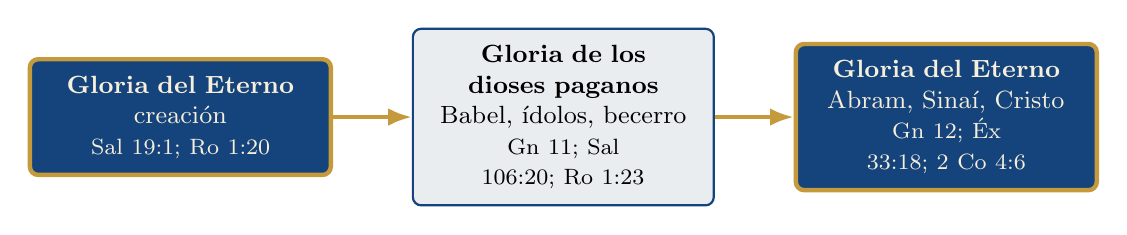
\begin{tikzpicture}[font=\small,node distance=1.0cm]
 \node[draw=dorado,line width=1.6pt,fill=azul,text=papiro,rounded corners=3pt,text width=3.4cm,align=center,inner sep=6pt] (a) {\textbf{Gloria del Eterno}\\ creación\\ \footnotesize Sal 19:1; Ro 1:20};
 \node[draw=azul,line width=0.8pt,fill=gris!12,rounded corners=3pt,text width=3.4cm,align=center,inner sep=6pt,right=of a] (b) {\textbf{Gloria de los dioses paganos}\\ Babel, ídolos, becerro\\ \footnotesize Gn 11; Sal 106:20; Ro 1:23};
 \node[draw=dorado,line width=1.6pt,fill=azul,text=papiro,rounded corners=3pt,text width=3.4cm,align=center,inner sep=6pt,right=of b] (c) {\textbf{Gloria del Eterno}\\ Abram, Sinaí, Cristo\\ \footnotesize Gn 12; Éx 33:18; 2 Co 4:6};
 \draw[-{Latex[length=3mm]},dorado,line width=1.4pt] (a)--(b);
 \draw[-{Latex[length=3mm]},dorado,line width=1.4pt] (b)--(c);
\end{tikzpicture}\par
{\footnotesize\color{gris}\textit{Figura 1.} De la gloria del Eterno a la gloria del Eterno. \textit{Nota.} Elaboración propia a partir del material de estudio de la serie.}
\end{center}

\hebverso{וְאֶעֶשְׂךָ לְגוֹי גָּדוֹל וַאֲבָרֶכְךָ וַאֲגַדְּלָה שְׁמֶךָ וֶהְיֵה בְּרָכָה}
\begin{verso}{Génesis 12:1–2}
Pero \SENOR{} había dicho a Abram: Vete de tu tierra y de tu parentela, y de la casa de tu padre, a la tierra que te mostraré. Y haré de ti una nación grande, y te bendeciré, y engrandeceré tu nombre, y serás bendición.
\end{verso}

En Babel el hombre quería ``hacerse un nombre'' (\heb{שֵׁם}, Gn 11:4); a Abram, Dios le dice: ``engrandeceré tu nombre'' (\heb{וַאֲגַדְּלָה שְׁמֶךָ}). El nombre que el hombre no pudo fabricarse, Dios lo da. Y cuando Abram llega a Canaán, el texto anota dónde estaba:

\begin{verso}{Génesis 12:6–7}
Y pasó Abram por aquella tierra hasta el lugar de Siquem, hasta el encino de More; y el cananeo estaba entonces en la tierra. Y apareció \SENOR{} a Abram, y le dijo: A tu descendencia daré esta tierra. Y edificó allí un altar a \SENOR, quien le había aparecido.
\end{verso}

En medio del culto cananeo, Abram levanta un altar al \SENOR. Es su primer ``no'' a los dioses de la tierra. Siglos después, en ese mismo lugar, Israel dirá ``sí'' a un dios cananeo (sección~\ref{sec:siquem}).

\precision{el contraste ``Babel busca un nombre / Abram lo recibe'' es común entre los comentaristas (Wenham, 1987). La lectura de Gn 12:6--7 como rechazo del culto cananeo de Siquem es propia de esta serie.}

%===================================================================
\section{Texto ancla: Éxodo 34:6--7}

\subsection{Después del becerro}
La revelación más completa del carácter de Dios en el Antiguo Testamento llega en el peor momento de Israel. Recién salidos de Egipto, ya en el pacto, fabrican un becerro de oro y dicen: ``Israel, estos son tus dioses, que te sacaron de la tierra de Egipto'' (Éx 32:4). Moisés rompe las tablas (32:19) e intercede: ``que perdones ahora su pecado, y si no, ráeme ahora de tu libro que has escrito'' (32:32). Y entonces pide algo inaudito:

\hebverso{הַרְאֵנִי נָא אֶת־כְּבֹדֶךָ \\ וְחַנֹּתִי אֶת־אֲשֶׁר אָחֹן וְרִחַמְתִּי אֶת־אֲשֶׁר אֲרַחֵם}
\begin{verso}{Éxodo 33:18–19}
El entonces dijo: Te ruego que me muestres tu gloria. Y le respondió: Yo haré pasar todo mi bien delante de tu rostro, y proclamaré el nombre de \SENOR{} delante de ti; y tendré misericordia del que tendré misericordia, y seré clemente para con el que seré clemente.
\end{verso}

\begin{filologia}{Éx 33:18--19}
\heb{כָּבוֹד} \emph{kavod} & \heb{כבד} & ``gloria'', literalmente ``peso'': Moisés pide ver el peso, la realidad de Dios. \\
\heb{טוּב} \emph{tuv} & \heb{טוב} & ``bien, bondad'': Dios responde al pedido de gloria con ``todo mi bien''. \\
\heb{וְחַנֹּתִי} \emph{vejannotí} & \heb{חנן} & ``tendré gracia'' de quien tendré gracia (RVR1960: ``tendré misericordia''). \\
\heb{וְרִחַמְתִּי} \emph{verijamtí} & \heb{רחם} & ``me compadeceré'' de quien me compadeceré (RVR1960: ``seré clemente''). \\
\end{filologia}

\precision{la RVR1960 invierte los términos: traduce \emph{janán} por ``misericordia'' y \emph{rajam} por ``clemente''. La construcción ``tendré gracia de quien tendré gracia'' (\emph{idem per idem}) es la misma de ``Yo soy el que soy'' (Éx 3:14): afirma la libertad soberana de Dios.}

\subsection{El Nombre proclamado}
Moisés sube de nuevo al Sinaí con dos tablas nuevas (Éx 34:4). Dios desciende en la nube y pasa delante de él:

\hebverso{וַיַּעֲבֹר יְהוָה עַל־פָּנָיו וַיִּקְרָא יְהוָה יְהוָה אֵל רַחוּם וְחַנּוּן \\ אֶרֶךְ אַפַּיִם וְרַב־חֶסֶד וֶאֱמֶת נֹצֵר חֶסֶד לָאֲלָפִים \\ נֹשֵׂא עָוֹן וָפֶשַׁע וְחַטָּאָה וְנַקֵּה לֹא יְנַקֶּה}
\begin{verso}{Éxodo 34:6–7}
Y pasando \SENOR{} por delante de él, proclamó: ¡\SENOR! ¡\SENOR! fuerte, misericordioso y piadoso; tardo para la ira, y grande en misericordia y verdad; que guarda misericordia a millares, que perdona la iniquidad, la rebelión y el pecado, y que de ningún modo tendrá por inocente al malvado; que visita la iniquidad de los padres sobre los hijos y sobre los hijos de los hijos, hasta la tercera y cuarta generación.
\end{verso}

\begin{filologia}{Éx 34:6--7}
\heb{אֵל} \emph{El} & --- & ``Dios'' (RVR1960: ``fuerte''). \\
\heb{רַחוּם} \emph{rajum} & \heb{רחם} & ``compasivo'', de \emph{réjem}, el vientre materno: la ternura de una madre por su hijo. \\
\heb{חַנּוּן} \emph{jannun} & \heb{חנן} & ``clemente, lleno de gracia'': el que se inclina con favor hacia quien no lo merece. \\
\heb{אֶרֶךְ אַפַּיִם} \emph{érej appáyim} & \heb{ארך}, \heb{אנף} & ``largo de narices'': lento para que la ira se encienda. \\
\heb{רַב־חֶסֶד וֶאֱמֶת} \emph{rav jésed ve'emet} & \heb{חסד}, \heb{אמן} & ``abundante en amor leal y en verdad'': los dos pilares del pacto. \\
\heb{נֹצֵר חֶסֶד לָאֲלָפִים} \emph{notser jésed la'alafim} & \heb{נצר} & ``que guarda (vigila, custodia) el amor leal para millares''. \\
\heb{נֹשֵׂא עָוֹן} \emph{nosé avón} & \heb{נשׂא} & ``que levanta, carga la iniquidad'': perdonar es cargar con la culpa del otro. \\
\heb{וְנַקֵּה לֹא יְנַקֶּה} \emph{venaqqé lo yenaqqé} & \heb{נקה} & ``y absolver, no absuelve'': el infinitivo absoluto refuerza la negación (RVR1960: ``de ningún modo tendrá por inocente''). \\
\end{filologia}

El Nombre tiene tres partes. Primero, \emph{lo que Dios es}: compasivo, clemente, lento para la ira, abundante en \emph{jésed} y verdad (v.~6). Segundo, \emph{lo que hace}: guarda el \emph{jésed} a millares y carga la iniquidad, la rebelión y el pecado (v.~7a). Tercero, \emph{lo que no hace}: no absuelve al culpable impenitente (v.~7b). Las proporciones hablan por sí mismas: \emph{jésed} para ``millares'' (de generaciones, como entiende Dt 7:9) frente a visitación hasta la tercera y cuarta. La misericordia es más grande que el juicio, sin anularlo.

\begin{verso}{Éxodo 34:8}
Entonces Moisés, apresurándose, bajó la cabeza hacia el suelo y adoró.
\end{verso}

Moisés había pedido ver la \emph{gloria} (33:18), y Dios le mostró su \emph{carácter}. Esa es la tesis de esta obra: la gloria de Dios es la comunión de sus atributos. En el Sinaí, esa comunión se anuncia con la misericordia en primer lugar.

\subsection{La fórmula que recorre la Biblia}
Israel no inventó un concepto nuevo de Dios en cada época: repitió el Nombre que Dios proclamó en el Sinaí. La fórmula de Éx 34:6 reaparece en la oración, en la alabanza y en la profecía.

\begin{center}\small\renewcommand{\arraystretch}{1.2}
\begin{tabular}{@{}L{2.3cm}L{8.8cm}L{3.6cm}@{}}
\toprule
\textbf{Texto} & \textbf{RVR1960} & \textbf{Uso} \\ \midrule
Nm 14:18--19 & ``\SENOR, tardo para la ira y grande en misericordia\ldots{} Perdona ahora la iniquidad de este pueblo según la grandeza de tu misericordia'' & Moisés intercede \\
Sal 86:15 & ``Mas tú, Señor, Dios misericordioso y clemente, lento para la ira, y grande en misericordia y verdad'' & oración personal \\
Sal 103:8 & ``Misericordioso y clemente es \SENOR; lento para la ira, y grande en misericordia'' & alabanza \\
Sal 145:8 & ``Clemente y misericordioso es \SENOR, lento para la ira, y grande en misericordia'' & alabanza (acróstico) \\
Jl 2:13 & ``porque misericordioso es y clemente, tardo para la ira y grande en misericordia'' & llamado al arrepentimiento \\
Jon 4:2 & ``sabía yo que tú eres Dios clemente y piadoso, tardo en enojarte, y de grande misericordia'' & queja del profeta \\
Nah 1:3 & ``\SENOR{} es tardo para la ira\ldots{} y no tendrá por inocente al culpable'' & juicio de Nínive \\
\bottomrule
\end{tabular}\par
{\footnotesize\color{gris}\textit{Tabla 2.} Ecos de Éx 34:6--7 en el Antiguo Testamento.}
\end{center}

%===================================================================
\section{La palabra: cuatro columnas}

La Escritura dice la misericordia con muchas palabras, pero cuatro de ellas, las del material de estudio, sostienen el techo. Ninguna basta sola; juntas muestran cómo Dios se acerca al que no merece (\emph{janán}), al que pertenece a su pacto (\emph{jésed}), al que sufre (\emph{rajamím}) y al que debería morir (\emph{jamal}).

\subsection{El espectro completo}\label{sec:espectro}
Antes de las cuatro columnas conviene ver el conjunto. Estos son todos los términos del texto original que la RVR1960 traduce con ``misericordia'', ``misericordias'', ``misericordioso'' o ``tener misericordia''.

\begin{center}\small\renewcommand{\arraystretch}{1.2}
\begin{tabular}{@{}L{1.3cm}L{4.6cm}L{4.4cm}L{4.0cm}@{}}
\toprule
\textbf{Raíz} & \textbf{Términos} & \textbf{Imagen y sentido} & \textbf{Textos} \\ \midrule
\heb{חסד} & \heb{חֶסֶד} \emph{jésed}; \heb{חָסִיד} \emph{jasid} ``misericordioso''; \heb{הִתְחַסֵּד} \emph{hitjassed} ``mostrarse misericordioso'' & lealtad del pacto; el \emph{jasid} es el que vive en \emph{jésed} & Éx 34:6; Sal 136; 2~S 22:26; Jer 3:12; Mi 7:2 \\
\heb{רחם} & \heb{רַחֲמִים} \emph{rajamím}; \heb{רָחַם} \emph{rajam}; \heb{רַחוּם} \emph{rajum} & el vientre (\emph{réjem}): ternura de entrañas & Sal 103:13; Jer 31:20; Os 2:23 \\
\heb{חנן} & \heb{חָנַן} \emph{janán}; \heb{חַנּוּן} \emph{jannun}; \heb{חֵן} \emph{jen}; \heb{תְּחִנָּה} \emph{tejinná}; \heb{תַּחֲנוּנִים} \emph{tajanunim} & inclinarse con favor; la gracia que se suplica & Sal 86:3; Pr 14:21; Jos 11:20; Esd 9:8; Jer 31:9 \\
\heb{חמל} & \heb{חָמַל} \emph{jamal}; \heb{חֶמְלָה} \emph{jemlá} & perdonar la vida, no destruir & Gn 19:16; Mal 3:17; Ez 5:11 \\
\heb{חוס} & \heb{חוּס} \emph{jus} & el ojo que ``tiene lástima'' & Sal 72:13; Jon 4:11; Ez 5:11 \\
\heb{נחם} & \heb{נִחַם} \emph{nijam} (nifal) & conmoverse hasta cambiar el curso & Jue 2:18 \\
\heb{טוב} & \heb{טוֹב־עַיִן} \emph{tov ayin} & ``bueno de ojo'': el generoso & Pr 22:9 \\
Arameo & \heb{רַחֲמִין} \emph{rajamín}; \heb{מִחַן} \emph{mijan} (de \heb{חֲנַן}) & compasión; hacer gracia al oprimido & Dn 2:18; 4:27 \\
\bottomrule
\end{tabular}\par
{\footnotesize\color{gris}\textit{Tabla 3.} Términos hebreos y arameos traducidos ``misericordia'' en la RVR1960. \textit{Nota.} Sentidos según Strong y Koehler y Baumgartner (2001).}
\end{center}

\begin{center}\small\renewcommand{\arraystretch}{1.2}
\begin{tabular}{@{}L{3.6cm}L{4.8cm}L{1.3cm}L{4.6cm}@{}}
\toprule
\textbf{Término} & \textbf{Sentido} & \textbf{Vv.} & \textbf{Textos} \\ \midrule
\grc{ἔλεος}, \grc{ἐλεέω} & misericordia; tener misericordia (en la LXX traduce \emph{jésed}) & 26; 28 & Mt 9:13; Ro 9:15; Ef 2:4 \\
\grc{ἐλεήμων} & misericordioso & 2 & Mt 5:7; He 2:17 \\
\grc{ἀνέλεος}, \grc{ἀνελεήμων} & sin misericordia & 1; 1 & Stg 2:13; Ro 1:31 \\
\grc{οἰκτιρμός}, \grc{οἰκτίρμων} & compasión; compasivo (LXX: \emph{rajamím}, \emph{rajum}) & 4; 2 & Ro 12:1; 2~Co 1:3; Lc 6:36 \\
\grc{σπλαγχνίζομαι} & conmoverse en las entrañas & 5 & Mt 18:27; Lc 10:33; 15:20 \\
\grc{σπλάγχνα} & ``entrañas'': ``entrañable misericordia'' & 3 & Lc 1:78; Flp 2:1; Col 3:12 \\
\grc{εὔσπλαγχνος} & ``de buenas entrañas'' & 2 & Ef 4:32; 1~P 3:8 \\
\grc{πολύσπλαγχνος} & ``de muchas entrañas'' & 1 & Stg 5:11 \\
\grc{ὅσιος} & \grc{τὰ ὅσια Δαυίδ}: las lealtades prometidas a David & 1 & Hch 13:34 (= Is 55:3, \emph{jasdé David}) \\
\bottomrule
\end{tabular}\par
{\footnotesize\color{gris}\textit{Tabla 4.} Términos griegos traducidos ``misericordia'' en la RVR1960. \textit{Nota.} Versículos según NA27 con números Strong; sentidos según BDAG.}
\end{center}

\precision{dos casos especiales del Nuevo Testamento: en Mt 21:41 ``sin misericordia'' traduce el adverbio \grc{κακῶς} (``malamente''), una traducción libre; en Tit 1:4, ``misericordia'' (\grc{ἔλεος}) está en el Texto Recibido que sigue la RVR1960, pero no en NA28. En hebreo, \emph{nijam} suele traducirse ``arrepentirse'' (de Dios: cambiar el curso anunciado); solo en Jue 2:18 la RVR1960 lo vierte ``era movido a misericordia''.}

\subsubsection*{Las palabras menores}
Cada término menor añade un matiz. El \emph{jasid} es el hombre en quien el \emph{jésed} se volvió carácter: ``Faltó el misericordioso de la tierra, y ninguno hay recto entre los hombres'' (Mi 7:2). Dios lo dice de sí mismo: ``misericordioso (\heb{חָסִיד}) soy yo, dice \SENOR, no guardaré para siempre el enojo'' (Jer 3:12). Y el salmo enseña que Dios responde en la misma moneda: ``Con el misericordioso te mostrarás misericordioso'' (\heb{עִם־חָסִיד תִּתְחַסָּד}, 2~S 22:26; Sal 18:25).

\emph{Tejinná} y \emph{tajanunim}, de la raíz \emph{janán}, son la gracia vista desde quien la pide. Esdras confiesa: ``por un breve momento ha habido misericordia (\heb{תְחִנָּה}) de parte de \SENOR{} nuestro Dios, para hacer que nos quedase un remanente libre'' (Esd 9:8). Jeremías dice del regreso de Efraín: ``Irán con lloro, mas con misericordia (\heb{וּבְתַחֲנוּנִים}, ``con súplicas'') los haré volver'' (Jer 31:9).

\emph{Jus} es el ojo que se apiada: ``Tendrá misericordia (\heb{יָחֹס}) del pobre y del menesteroso'' (Sal 72:13); en el juicio se dice lo contrario: ``mi ojo no perdonará (\heb{תָחוֹס}), ni tampoco tendré yo misericordia (\heb{אֶחְמוֹל})'' (Ez 5:11), donde \emph{jus} y \emph{jamal} van juntos. \emph{Nijam} describe a Dios conmovido por el dolor de su pueblo: ``\SENOR{} era movido a misericordia (\heb{יִנָּחֵם}) por sus gemidos'' (Jue 2:18). Y \emph{tov ayin}, ``bueno de ojo'', llama misericordioso al generoso: ``El ojo misericordioso será bendito, porque dio de su pan al indigente'' (Pr 22:9).

En arameo, Daniel y sus compañeros piden ``misericordias'' (\heb{רַחֲמִין}) al Dios del cielo (Dn 2:18), y Daniel aconseja a Nabucodonosor redimir sus iniquidades ``haciendo misericordias para con los oprimidos'' (\heb{בְּמִחַן עֲנָיִן}, Dn 4:27).

En griego, la familia de \grc{σπλάγχνα} (``entrañas'') traduce la imagen de \emph{rajamím}: Zacarías canta ``la entrañable misericordia de nuestro Dios'' (\grc{διὰ σπλάγχνα ἐλέους θεοῦ ἡμῶν}, Lc 1:78); Pablo pide vestirse ``de entrañable misericordia'' (\grc{σπλάγχνα οἰκτιρμοῦ}, Col 3:12) y ser ``misericordiosos'' (\grc{εὔσπλαγχνοι}, ``de buenas entrañas'', Ef 4:32); Santiago confiesa que ``el Señor es muy misericordioso (\grc{πολύσπλαγχνος}) y compasivo'' (Stg 5:11), eco de Éx 34:6. Hebreos llama a Cristo ``misericordioso y fiel sumo sacerdote'' (\grc{ἐλεήμων καὶ πιστός}, He 2:17): el par \emph{jésed ve'emet} hecho persona. Y en Antioquía de Pisidia, Pablo anuncia la resurrección con Is 55:3: ``Os daré las misericordias fieles de David'' (\grc{τὰ ὅσια Δαυὶδ τὰ πιστά}, Hch 13:34), donde la LXX traduce \heb{חַסְדֵי דָוִד הַנֶּאֱמָנִים}. El \emph{jésed} prometido a David se cumple en el Resucitado.

\precision{colosenses y Efesios son de autoría paulina discutida; Hebreos no es de Pablo; Hch 13:34 recoge un discurso de Pablo según Lucas.}

De todo el espectro, cuatro palabras son las columnas que sostienen el techo.

\subsection{\emph{Janán}: gracia, favor inmerecido}
\hebverso{יָאֵר יְהוָה פָּנָיו אֵלֶיךָ וִיחֻנֶּךָּ}
\begin{verso}{Números 6:25}
\SENOR{} haga resplandecer su rostro sobre ti, y tenga de ti misericordia.
\end{verso}

\hebverso{חָנֵּנִי אֲדֹנָי כִּי אֵלֶיךָ אֶקְרָא כָּל־הַיּוֹם}
\begin{verso}{Salmo 86:3}
Ten misericordia de mí, oh Señor; Porque a ti clamo todo el día.
\end{verso}

\begin{filologia}{Nm 6:25 y Sal 86:3}
\heb{וִיחֻנֶּךָּ} \emph{viyjunnekka} & \heb{חנן} & ``y te otorgue gracia''. \emph{Janán} (Strong H2603) es ``inclinarse en bondad hacia un inferior''. \\
\heb{חָנֵּנִי} \emph{jonnení} & \heb{חנן} & ``ten gracia de mí'': imperativo del que no tiene derechos que reclamar. \\
\heb{חֵן}, \heb{תְּחִנָּה} \emph{jen}, \emph{tejinná} & \heb{חנן} & ``gracia'' y ``súplica''. La forma reflexiva del verbo (\emph{hitjanén}) significa \emph{implorar}: pedir gracia. \\
\end{filologia}

En la bendición sacerdotal, la gracia va unida al rostro de Dios que resplandece. En el Salmo, el que no tiene méritos clama ``todo el día''. Y en Éx 33:19 Dios afirma que su gracia es libre: ``tendré gracia de quien tendré gracia''.

La libertad de esa gracia tiene un eco en el Nuevo Testamento. Cuando Pedro, después de ser restaurado, pregunta por el destino de Juan, Jesús le responde:

\begin{verso}{Juan 21:21–22}
Cuando Pedro le vio, dijo a Jesús: Señor, ¿y qué de éste? Jesús le dijo: Si quiero que él quede hasta que yo venga, ¿qué a ti? Sígueme tú.
\end{verso}

\precision{la conexión entre Éx 33:19 y Jn 21:22 es del autor de la serie y es una lectura propia: la gracia de Dios no se administra con criterio humano; a cada uno le toca recibirla y seguir.}

La parábola del siervo que no perdonó muestra la gracia en su forma más pura:

\begin{verso}{Mateo 18:26–27}
Entonces aquel siervo, postrado, le suplicaba, diciendo: Señor, ten paciencia conmigo, y yo te lo pagaré todo. El señor de aquel siervo, movido a misericordia, le soltó y le perdonó la deuda.
\end{verso}

Diez mil talentos (Mt 18:24) era una deuda imposible de pagar. El siervo implora, y el rey no le da más plazo: le perdona todo. El verbo es \grc{σπλαγχνισθείς}, ``conmovido en las entrañas''.

\subsection{\emph{Rajamím}: compasión desde las entrañas}
\hebverso{כְּרַחֵם אָב עַל־בָּנִים רִחַם יְהוָה עַל־יְרֵאָיו}
\begin{verso}{Salmo 103:13}
Como el padre se compadece de los hijos, Se compadece \SENOR{} de los que le temen.
\end{verso}

\begin{filologia}{Sal 103:13}
\heb{רֶחֶם} \emph{réjem} & \heb{רחם} & ``vientre, matriz'' (H7358). \\
\heb{רַחֲמִים} \emph{rajamím} & \heb{רחם} & plural de \emph{réjem}: ``entrañas'' y, por extensión, ``compasión'' (H7356). Es el amor que se siente en el cuerpo, como el de la madre de 1~R 3:26, a quien ``sus entrañas se le conmovieron por su hijo''. \\
\heb{כְּרַחֵם}\ldots{} \heb{רִחַם} \emph{kerajem\ldots{} rijam} & \heb{רחם} & ``como se compadece\ldots{} se compadece'': el paralelismo compara la compasión del padre con la de Dios. \\
\end{filologia}

El Salmo aplica a un padre una imagen que nace del vientre materno: la ternura de Dios reúne la de la madre y la del padre. Jeremías la lleva más lejos:

\hebverso{הֲבֵן יַקִּיר לִי אֶפְרַיִם אִם יֶלֶד שַׁעֲשֻׁעִים \\ עַל־כֵּן הָמוּ מֵעַי לוֹ רַחֵם אֲרַחֲמֶנּוּ נְאֻם־יְהוָה}
\begin{verso}{Jeremías 31:18–20}
Escuchando, he oído a Efraín que se lamentaba: Me azotaste, y fui castigado como novillo indómito; conviérteme, y seré convertido, porque tú eres \SENOR{} mi Dios. Porque después que me aparté tuve arrepentimiento, y después que reconocí mi falta, herí mi muslo; me avergoncé y me confundí, porque llevé la afrenta de mi juventud. ¿No es Efraín hijo precioso para mí? ¿no es niño en quien me deleito? pues desde que hablé de él, me he acordado de él constantemente. Por eso mis entrañas se conmovieron por él; ciertamente tendré de él misericordia, dice \SENOR.
\end{verso}

\begin{filologia}{Jer 31:20}
\heb{הָמוּ מֵעַי} \emph{hamú me'ay} & \heb{המה} & ``mis entrañas se agitaron'': el verbo describe el bramido del mar y el ruido de una multitud. \\
\heb{רַחֵם אֲרַחֲמֶנּוּ} \emph{rajem arajamennu} & \heb{רחם} & ``compadecer, me compadeceré de él'': el infinitivo absoluto intensifica (RVR1960: ``ciertamente''). \\
\end{filologia}

Efraín, el reino del norte, había sido castigado ``como novillo indómito''; la palabra es \heb{עֵגֶל} (\emph{éguel}), la misma del becerro de Éx 32. El hijo vuelve avergonzado, y el Padre confiesa que sus entrañas se agitan por él. Jesús contó la misma escena:

\begin{verso}{Lucas 15:20}
Y levantándose, vino a su padre. Y cuando aún estaba lejos, lo vio su padre, y fue movido a misericordia, y corrió, y se echó sobre su cuello, y le besó.
\end{verso}

El verbo \grc{ἐσπλαγχνίσθη} (\emph{esplanjnísthē}) viene de \grc{σπλάγχνα}, ``entrañas'': es el equivalente griego de \emph{rajamím}. El padre de la parábola actúa como el Dios de Jer 31:20. Y Jesús mismo se conmueve ante el dolor: ante la tumba de Lázaro ``se estremeció en espíritu y se conmovió\ldots{} Jesús lloró'' (Jn 11:33, 35).

\precision{jn 11:33 no usa \grc{σπλαγχνίζομαι}, sino \grc{ἐνεβριμήσατο} (``se estremeció'') y \grc{ἐτάραξεν ἑαυτόν} (``se turbó''); el v.~35 dice \grc{ἐδάκρυσεν} (``lloró''). El verbo de las entrañas aplicado a Jesús aparece en los sinópticos (Mt 9:36; 14:14; Lc 7:13).}

\subsection{\emph{Jamal}: perdonar la vida, levantar}
\hebverso{בְּחֶמְלַת יְהוָה עָלָיו}
\begin{verso}{Génesis 19:16}
Y deteniéndose él, los varones asieron de su mano, y de la mano de su mujer y de las manos de sus dos hijas, según la misericordia de \SENOR{} para con él; y lo sacaron y lo pusieron fuera de la ciudad.
\end{verso}

\hebverso{וְחָמַלְתִּי עֲלֵיהֶם כַּאֲשֶׁר יַחְמֹל אִישׁ עַל־בְּנוֹ הָעֹבֵד אֹתוֹ}
\begin{verso}{Malaquías 3:17}
Y serán para mí especial tesoro, ha dicho \SENOR{} de los ejércitos, en el día en que yo actúe; y los perdonaré, como el hombre que perdona a su hijo que le sirve.
\end{verso}

\begin{filologia}{Gn 19:16 y Mal 3:17}
\heb{חֶמְלָה} \emph{jemlá} & \heb{חמל} & ``compasión, piedad'' (Gn 19:16): la que libra de la destrucción. \\
\heb{וְחָמַלְתִּי} \emph{vejamaltí} & \heb{חמל} & ``y tendré piedad, los perdonaré'' (Mal 3:17). \emph{Jamal} (H2550) significa compadecerse y, por implicación, librar, perdonar la vida, no destruir. \\
\end{filologia}

\emph{Jamal} es la misericordia que \emph{saca} del lugar del juicio. Lot ``se demoraba''; la misericordia lo toma de la mano y lo pone fuera de Sodoma. En Malaquías, Dios ``perdona'' a los suyos en el día del juicio como un padre que preserva a su hijo.

Jonás termina con una pregunta de Dios que usa un sinónimo cercano:

\hebverso{וַאֲנִי לֹא אָחוּס עַל־נִינְוֵה הָעִיר הַגְּדוֹלָה}
\begin{verso}{Jonás 4:10–11}
Y dijo \SENOR: Tuviste tú lástima de la calabacera, en la cual no trabajaste, ni tú la hiciste crecer; que en espacio de una noche nació, y en espacio de otra noche pereció. ¿Y no tendré yo piedad de Nínive, aquella gran ciudad donde hay más de ciento veinte mil personas que no saben discernir entre su mano derecha y su mano izquierda, y muchos animales?
\end{verso}

\precision{jon 4:10--11 no usa \emph{jamal}, sino \heb{חוּס} (\emph{jus}, H2347), ``tener lástima, perdonar la vida''. Jonás ``tuvo lástima'' de una planta; Dios, de una ciudad entera y hasta de sus animales. El libro termina con la pregunta sin respuesta: la deja al lector.}

\subsection{\emph{Jésed}: amor leal del pacto}
\hebverso{חַסְדֵי יְהוָה כִּי לֹא־תָמְנוּ כִּי לֹא־כָלוּ רַחֲמָיו \\ חֲדָשִׁים לַבְּקָרִים רַבָּה אֱמוּנָתֶךָ}
\begin{verso}{Lamentaciones 3:22–23}
Por la misericordia de \SENOR{} no hemos sido consumidos, porque nunca decayeron sus misericordias. Nuevas son cada mañana; grande es tu fidelidad.
\end{verso}

\hebverso{כָּל־אָרְחוֹת יְהוָה חֶסֶד וֶאֱמֶת לְנֹצְרֵי בְרִיתוֹ וְעֵדֹתָיו}
\begin{verso}{Salmo 25:10}
Todas las sendas de \SENOR{} son misericordia y verdad, Para los que guardan su pacto y sus testimonios.
\end{verso}

\begin{filologia}{Lam 3:22 y Sal 25:10}
\heb{חֶסֶד} \emph{jésed} & \heb{חסד} & bondad leal, amor que se mantiene por compromiso (H2617). Es la palabra del pacto: la lealtad que Dios jura y cumple. \\
\heb{חַסְדֵי} \emph{jasdé} & \heb{חסד} & ``las misericordias (de)'': plural de \emph{jésed}; junto a \heb{רַחֲמָיו} \emph{rajamav}, ``sus compasiones'' (Lam 3:22). \\
\heb{בְּרִית} \emph{berit} & --- & ``pacto'' (Sal 25:10): el \emph{jésed} se vive dentro de un pacto. \\
\end{filologia}

Lamentaciones 3 es un acróstico triple (tres versos por cada letra del alfabeto), y estos versos están en el centro del libro, escritos entre las ruinas de Jerusalén. En medio del juicio, el poeta encuentra que el \emph{jésed} no se agotó.

\precision{\emph{Jésed} no tiene equivalente exacto en español. La RVR1960 lo traduce ``misericordia'' 205 veces, pero también ``bondad'', ``benignidad'', ``favor'' y ``fidelidad'' (Strong H2617).}

En Oseas, \emph{jésed} es lo que Dios espera de su pueblo:

\hebverso{כִּי חֶסֶד חָפַצְתִּי וְלֹא־זָבַח וְדַעַת אֱלֹהִים מֵעֹלוֹת}
\begin{verso}{Oseas 6:6}
Porque misericordia quiero, y no sacrificio, y conocimiento de Dios más que holocaustos.
\end{verso}

Dos versos antes, Dios se queja: ``La piedad vuestra (\emph{jésed}) es como nube de la mañana'' (Os 6:4). Jesús cita Os 6:6 dos veces (Mt 9:13; 12:7). La LXX traduce \emph{jésed} con \grc{ἔλεος}: \grc{διότι ἔλεος θέλω καὶ οὐ θυσίαν}. El puente entre los testamentos es directo: \emph{jésed} $\rightarrow$ \emph{éleos}.

\subsection{Del hebreo a Pablo}
La Septuaginta tradujo el Nombre de Éx 34:6 así: \grc{κύριος ὁ θεὸς οἰκτίρμων καὶ ἐλεήμων, μακρόθυμος καὶ πολυέλεος καὶ ἀληθινός}. Ese vocabulario pasa a Pablo.

\begin{center}
\begin{tikzpicture}[font=\small,node distance=0.8cm]
 \node[draw=azul,line width=0.8pt,fill=papiro,rounded corners=3pt,text width=3.6cm,align=center,inner sep=5pt] (h) {\textbf{Hebreo (Éx 34:6)}\\ \heb{רַחוּם} \emph{rajum}\\ \heb{חַנּוּן} \emph{jannun}\\ \heb{רַב־חֶסֶד} \emph{rav jésed}};
 \node[draw=azul,line width=0.8pt,fill=papiro,rounded corners=3pt,text width=3.6cm,align=center,inner sep=5pt,right=of h] (l) {\textbf{Septuaginta}\\ \grc{οἰκτίρμων}\\ \grc{ἐλεήμων}\\ \grc{πολυέλεος}};
 \node[draw=azul,line width=0.8pt,fill=papiro,rounded corners=3pt,text width=4.2cm,align=center,inner sep=5pt,right=of l] (p) {\textbf{Pablo}\\ \grc{πατὴρ τῶν οἰκτιρμῶν} (2 Co 1:3)\\ \grc{πλούσιος ἐν ἐλέει} (Ef 2:4)\\ \grc{ἐλεήσω ὃν ἂν ἐλεῶ} (Ro 9:15)};
 \draw[-{Latex[length=2.5mm]},dorado,line width=1.2pt] (h)--(l);
 \draw[-{Latex[length=2.5mm]},dorado,line width=1.2pt] (l)--(p);
\end{tikzpicture}\par
{\footnotesize\color{gris}\textit{Figura 2.} Del Nombre de Éx 34:6 al vocabulario de Pablo. \textit{Nota.} Elaboración propia (BHS, LXX, NA28).}
\end{center}

\begin{filologia}{El vocabulario griego}
\grc{ἔλεος} \emph{éleos} & --- & compasión activa ante la miseria; en la LXX traduce casi siempre \emph{jésed} (BDAG). \\
\grc{οἰκτιρμός} \emph{oiktirmós} & \grc{οἰκτίρω} & compasión, piedad que se conmueve; en la LXX traduce sobre todo \emph{rajamím}. \\
\grc{σπλαγχνίζομαι} \emph{splanjnízomai} & \grc{σπλάγχνα} & conmoverse en las entrañas; solo en los evangelios. \\
\end{filologia}

%===================================================================
\section{Definición}

\begin{tcolorbox}[colback=papiro,colframe=azul,boxrule=1pt,arc=3pt,fonttitle=\bfseries,title=Definición]
La misericordia de Dios es la perfección eterna por la cual Dios, movido desde sus entrañas y fiel a su pacto, se inclina hacia el miserable y el culpable para aliviarlo, perdonarlo y levantarlo, sin dejar de ser justo (Éx 34:6--7).
\end{tcolorbox}

\begin{center}\small\renewcommand{\arraystretch}{1.2}
\begin{tabular}{@{}L{3.4cm}L{6.6cm}L{4.4cm}@{}}
\toprule
\textbf{Rasgo} & \textbf{Qué afirma} & \textbf{Textos} \\ \midrule
Libre (\emph{janán}) & no se merece ni se exige & Éx 33:19; Ro 9:15 \\
Leal (\emph{jésed}) & se apoya en el pacto & Sal 25:10; Lam 3:22 \\
Tierna (\emph{rajamím}) & nace de las entrañas & Sal 103:13; Jer 31:20 \\
Que salva (\emph{jamal}) & saca del lugar del juicio & Gn 19:16; Mal 3:17 \\
Justa & no absuelve al impenitente & Éx 34:7; Nm 14:18 \\
\bottomrule
\end{tabular}\end{center}

\textbf{Clasificación.} La misericordia pertenece a los atributos de la \emph{relación con el ser humano}: responde a la pregunta ``¿cómo se revela Dios?''. Es eterna como todas sus perfecciones (``para siempre es su misericordia'', Sal 136:1), aunque se ejerce sobre criaturas que sufren. Es un atributo \emph{comunicable}: ``Sed, pues, misericordiosos, como también vuestro Padre es misericordioso'' (Lc 6:36).

\subsection{Misericordia y gracia}
Pink explica que la misericordia tiene su origen en la bondad de Dios. La bondad da a la criatura por el solo hecho de ser criatura; la misericordia es ``la pronta inclinación de Dios a aliviar la miseria de las criaturas caídas. Así, la misericordia presupone el pecado'' (Pink, 2020, cap. 14). Para distinguirla de la gracia, Pink recurre a los ángeles que no cayeron: Dios los eligió y los preservó, de modo que reciben gracia; pero nunca han recibido misericordia, porque nunca la necesitaron.

La distinción puede resumirse así: la gracia mira al \emph{culpable} que no merece; la misericordia mira al \emph{miserable} que sufre. En el hombre caído ambas cosas coinciden, y por eso Hebreos las junta: ``Acerquémonos, pues, confiadamente al trono de la gracia, para alcanzar misericordia y hallar gracia para el oportuno socorro'' (He 4:16).

\subsection{Siempre juntas: \emph{jésed} y \emph{emet}}
\hebverso{חֶסֶד־וֶאֱמֶת נִפְגָּשׁוּ צֶדֶק וְשָׁלוֹם נָשָׁקוּ}
\begin{verso}{Salmo 85:10 [85:11]}
La misericordia y la verdad se encontraron; La justicia y la paz se besaron.
\end{verso}

\begin{filologia}{Sal 85:10 (85:11)}
\heb{אֱמֶת} \emph{emet} & \heb{אמן} & ``firmeza, fidelidad, verdad'': lo que hace confiable el \emph{jésed}. \\
\heb{נִפְגָּשׁוּ} \emph{nifgashu} & \heb{פגשׁ} & ``se encontraron'', como dos personas que salen una al encuentro de la otra. \\
\end{filologia}

El par \emph{jésed ve'emet} aparece desde Éx 34:6 y recorre la Escritura: ``todas las sendas de \SENOR{} son misericordia y verdad'' (Sal 25:10); ``cumplirás la verdad a Jacob, y a Abraham la misericordia'' (Mi 7:20). Juan describe al Verbo encarnado ``lleno de gracia y de verdad'' (Jn 1:14). Misericordia sin verdad sería sentimentalismo; verdad sin misericordia, dureza. En Dios van siempre juntas.

\precision{leer ``lleno de gracia y de verdad'' (Jn 1:14) como eco de \emph{rav jésed ve'emet} es una lectura extendida entre los comentaristas (Carson, 1991).}

%===================================================================
\section{Teología: la exposición de Pink}

Pink dedica dos capítulos a este atributo: ``La misericordia de Dios'' y ``La tierna misericordia de Dios'' (Pink, 2020, caps. 14--15). Se usa aquí como referencia, sin seguir su orden.

\begin{verso}{Salmo 136:1}
Alabad a \SENOR, porque él es bueno; porque para siempre es su misericordia.
\end{verso}

Pink abre con el Salmo 136, que repite ``porque para siempre es su misericordia'' en sus 26 versos: la creación, el éxodo, el desierto y la entrada en la tierra se leen como obras del \emph{jésed}. Sus ideas principales son cinco:

\begin{enumerate}
\item La misericordia se origina en la bondad divina y presupone la miseria del pecado.
\item Hay que distinguir tres niveles: una misericordia \emph{general}, sobre toda la creación (``sus misericordias sobre todas sus obras'', Sal 145:9); una misericordia \emph{especial} hacia todos los hombres, a pesar de sus pecados (Mt 5:45); y una misericordia \emph{soberana}, reservada para los herederos de la salvación y comunicada en forma de pacto por medio del Mediador.
\item Dios nunca deja de ser misericordioso, porque es una cualidad de su esencia (Sal 116:5), pero el \emph{ejercicio} de su misericordia lo regula su voluntad soberana (Ro 9:15). Hablar de ``merecer'' misericordia es una contradicción (Tit 3:5).
\item Es una presunción ``diabólica'' seguir pecando contando con la misericordia, porque Dios ha dicho que ``de ningún modo dará por inocente al malvado'' (Éx 34:7). ``Dios muestra misericordia a los verdaderamente penitentes, pero no a los impenitentes'' (Pink, 2020, cap. 14).
\item La ``tierna misericordia'' (\emph{jésed}) de Dios hacia su pueblo está unida a su verdad y a su pacto: ``Mas no quitaré de él mi misericordia, ni falsearé mi verdad. No olvidaré mi pacto'' (Sal 89:33--34). Por eso es motivo de adoración, consuelo en el abatimiento y argumento en la oración (Sal 51:1; 119:76).
\end{enumerate}

\precision{resumen propio de Pink (2020, caps. 14--15). Pink observa también que ningún pueblo antiguo atribuyó a sus dioses una ternura semejante; esa observación coincide con el arco de la sección 2 (de la gloria de los dioses a la gloria del Eterno), pero es un juicio general suyo.}

%===================================================================
\section{Un encuentro en la historia de Israel: Moisés en el Sinaí}

El encuentro que define este atributo es el del texto ancla, leído ahora como historia. Moisés intercede tres veces. La primera, recién bajado del monte, se ofrece en lugar del pueblo:

\begin{verso}{Éxodo 32:31–32}
Entonces volvió Moisés a \SENOR, y dijo: Te ruego, pues este pueblo ha cometido un gran pecado, porque se hicieron dioses de oro, que perdones ahora su pecado, y si no, ráeme ahora de tu libro que has escrito.
\end{verso}

La segunda es el pedido de ver la gloria (Éx 33:18). La tercera llega inmediatamente después de oír el Nombre:

\hebverso{אִם־נָא מָצָאתִי חֵן בְּעֵינֶיךָ אֲדֹנָי יֵלֶךְ־נָא אֲדֹנָי בְּקִרְבֵּנוּ \\ כִּי עַם־קְשֵׁה־עֹרֶף הוּא וְסָלַחְתָּ לַעֲוֹנֵנוּ וּלְחַטָּאתֵנוּ וּנְחַלְתָּנוּ}
\begin{verso}{Éxodo 34:9}
Y dijo: Si ahora, Señor, he hallado gracia en tus ojos, vaya ahora el Señor en medio de nosotros; porque es un pueblo de dura cerviz; y perdona nuestra iniquidad y nuestro pecado, y tómanos por tu heredad.
\end{verso}

\begin{filologia}{Éx 34:9}
\heb{חֵן} \emph{jen} & \heb{חנן} & ``gracia'': Moisés apela a la gracia que él mismo halló. \\
\heb{כִּי עַם־קְשֵׁה־עֹרֶף} \emph{ki am-qeshé óref} & \heb{קשׁה} & ``porque es un pueblo duro de cerviz''. La conjunción \emph{ki} puede leerse ``porque'' o ``aunque''; la RVR1960 dice ``porque''. \\
\heb{וְסָלַחְתָּ} \emph{vesalajtá} & \heb{סלח} & ``y perdonarás'': el verbo del perdón que solo tiene a Dios por sujeto en la Biblia hebrea. \\
\end{filologia}

Moisés usa como argumento lo que haría desistir a cualquiera: la dureza del pueblo. Si la misericordia dependiera de la calidad de Israel, no habría esperanza; precisamente porque el pueblo es duro, necesita un Dios ``tardo para la ira y grande en misericordia''. Dios responde: ``He aquí, yo hago pacto'' (Éx 34:10).

Moisés aprendió en el Sinaí a orar con las palabras que Dios había dicho de sí mismo. Cuando el pueblo se rebela otra vez tras el informe de los espías, cita el Nombre:

\hebverso{סְלַח־נָא לַעֲוֹן הָעָם הַזֶּה כְּגֹדֶל חַסְדֶּךָ}
\begin{verso}{Números 14:19–20}
Perdona ahora la iniquidad de este pueblo según la grandeza de tu misericordia, y como has perdonado a este pueblo desde Egipto hasta aquí. Entonces \SENOR{} dijo: Yo lo he perdonado conforme a tu dicho.
\end{verso}

Moisés no apela a la bondad de Israel, sino al carácter de Dios. Ese patrón (orar con el Nombre) es el que la tradición judía convirtió en el centro de su oración de perdón.

%===================================================================
\section{La misericordia en el judaísmo}

\subsection{Las trece medidas}
La tradición judía llama a Éx 34:6--7 las \emph{shelosh esré middot} (\heb{שְׁלֹשׁ עֶשְׂרֵה מִדּוֹת}), ``las trece medidas (o atributos) de misericordia''. La cuenta más conocida es la de Rabbenu Tam, que recogen los Tosafot al Talmud (\emph{Rosh Hashaná} 17b): los dos nombres iniciales son dos medidas distintas, la misericordia de Dios antes de que el hombre peque y después de que peque y se arrepienta.

\begin{center}\small\renewcommand{\arraystretch}{1.15}
\begin{tabular}{@{}cL{4.2cm}L{5.8cm}@{}}
\toprule
\textbf{N.º} & \textbf{Hebreo} & \textbf{Sentido} \\ \midrule
1 & \heb{יְהוָה} & \SENOR{} (misericordia antes del pecado) \\
2 & \heb{יְהוָה} & \SENOR{} (misericordia después del arrepentimiento) \\
3 & \heb{אֵל} & Dios, poderoso en misericordia \\
4 & \heb{רַחוּם} & compasivo \\
5 & \heb{וְחַנּוּן} & y clemente \\
6 & \heb{אֶרֶךְ אַפַּיִם} & lento para la ira \\
7 & \heb{וְרַב־חֶסֶד} & y abundante en \emph{jésed} \\
8 & \heb{וֶאֱמֶת} & y verdad \\
9 & \heb{נֹצֵר חֶסֶד לָאֲלָפִים} & que guarda el \emph{jésed} para millares \\
10 & \heb{נֹשֵׂא עָוֹן} & que carga la iniquidad (pecado intencional) \\
11 & \heb{וָפֶשַׁע} & y la rebelión \\
12 & \heb{וְחַטָּאָה} & y el pecado (sin intención) \\
13 & \heb{וְנַקֵּה} & y absuelve \\
\bottomrule
\end{tabular}\par
{\footnotesize\color{gris}\textit{Tabla 5.} Las trece medidas según Rabbenu Tam. \textit{Nota.} Tosafot a \emph{Rosh Hashaná} 17b (Sefaria).}
\end{center}

\precision{la cuenta no es única. Según los mismos Tosafot, Rabbenu Nissim no cuenta el primer nombre, porque hay una pausa entre los dos, y divide ``que guarda el \emph{jésed}'' y ``para millares''. La imagen del material de estudio sigue otra cuenta, que empieza en \emph{El}. La medida 13 (``y absuelve'') se obtiene cortando la frase \emph{venaqqé lo yenaqqé} (``absolver, no absuelve''): es una lectura rabínica, no el sentido llano del verso.}

\subsection{“Les mostró el orden de la oración”}
El Talmud comenta así Éx 34:6, ``Y pasando el \SENOR{} por delante de él, proclamó'':

\precision{lo que sigue es interpretación rabínica, tomada del Talmud de Babilonia (\emph{Rosh Hashaná} 17b) según la edición William Davidson en Sefaria (Steinsaltz, 2017).}

Rabí Yojanán dice que, si el verso no estuviera escrito, sería imposible decirlo: enseña que el Santo, bendito sea, se envolvió en un manto de oración como el que dirige la oración de la congregación, y le mostró a Moisés el orden de la oración. Le dijo:

\hebverso{כׇּל זְמַן שֶׁיִּשְׂרָאֵל חוֹטְאִין יַעֲשׂוּ לְפָנַי כַּסֵּדֶר הַזֶּה וַאֲנִי מוֹחֵל לָהֶם}

``Siempre que Israel peque, que hagan delante de mí conforme a este orden, y yo los perdonaré.'' Rav Yehudá añade:

\hebverso{בְּרִית כְּרוּתָה לִשְׁלֹשׁ עֶשְׂרֵה מִדּוֹת שֶׁאֵינָן חוֹזְרוֹת רֵיקָם}

``Hay un pacto hecho con las trece medidas: no vuelven vacías'', y lo prueba con Éx 34:10: ``He aquí, yo hago pacto''. Rashi, en su comentario a Éx 34:6, resume la primera idea: ``\SENOR, \SENOR'' es la medida de misericordia, una vez antes de que el hombre peque y otra después de que peque y se arrepienta.

La lógica es la misma de Moisés en Nm 14:18--19: el que pecó ora con las palabras que Dios dijo de sí mismo.

\subsection{La medida de misericordia y la medida del juicio}
Los sabios distinguen dos ``medidas'' en Dios: \heb{מִדַּת הָרַחֲמִים} (\emph{middat harajamim}), la medida de misericordia, unida al nombre \heb{יְהוָה}, y \heb{מִדַּת הַדִּין} (\emph{middat haddín}), la medida del juicio, unida a \emph{Elohim}. Rashi, comentando Gn 1:1, explica que primero ``surgió en el pensamiento'' de Dios crear el mundo con la medida del juicio; al ver que el mundo no podría subsistir, ``antepuso la medida de misericordia y la asoció a la medida del juicio''. En el Talmud, Dios es llamado con frecuencia \heb{רַחֲמָנָא} (\emph{Rajmaná}), ``el Misericordioso''.

El Targum Ónkelos, la traducción aramea de la Torá, vierte Éx 34:6--7 así:

\hebverso{וְאַעְבַּר יְיָ שְׁכִנְתֵּיהּ עַל אַפּוֹהִי וּקְרָא יְיָ יְיָ אֱלָהָא רַחֲמָנָא וְחַנָּנָא}

``Y el \SENOR{} hizo pasar su \emph{Shejiná} (presencia) delante de él, y proclamó: \SENOR, \SENOR, Dios misericordioso y clemente''. Y donde el hebreo dice ``y absolver, no absuelve'', Ónkelos traduce:

\hebverso{סָלַח לִדְתַיְבִין לְאוֹרַיְתֵיהּ וְלִדְלָא תַיְבִין לָא מְזַכֵּי}

``Perdona a los que vuelven a su Torá, y a los que no vuelven no los absuelve''.

\precision{son lecturas rabínicas (Targum Ónkelos según Sefaria). Ónkelos resuelve la tensión de Éx 34:7 con el arrepentimiento, igual que Pink: ``Dios muestra misericordia a los verdaderamente penitentes, pero no a los impenitentes'' (Pink, 2020, cap. 14).}

\subsection{En la oración y en el calendario}
Las trece medidas son el centro de las \emph{selijot} (\heb{סְלִיחוֹת}), las oraciones penitenciales que se recitan antes de Rosh Hashaná y en los días de ayuno (Elbogen, 1993). En Yom Kipur se repiten a lo largo del día, hasta la oración final (\emph{Neilá}). En la tarde de ese día se lee el libro de Jonás (\emph{Meguilá} 31a): la misericordia de Dios con Nínive, leída en el día del perdón de Israel. En Rosh Hashaná, en el rito del \emph{Tashlij}, se recita junto a aguas corrientes el final de Miqueas:

\hebverso{מִי־אֵל כָּמוֹךָ נֹשֵׂא עָוֹן וְעֹבֵר עַל־פֶּשַׁע לִשְׁאֵרִית נַחֲלָתוֹ \\ לֹא־הֶחֱזִיק לָעַד אַפּוֹ כִּי־חָפֵץ חֶסֶד הוּא}
\begin{verso}{Miqueas 7:18–19}
¿Qué Dios como tú, que perdona la maldad, y olvida el pecado del remanente de su heredad? No retuvo para siempre su enojo, porque se deleita en misericordia. El volverá a tener misericordia de nosotros; sepultará nuestras iniquidades, y echará en lo profundo del mar todos nuestros pecados.
\end{verso}

\begin{filologia}{Mi 7:18}
\heb{נֹשֵׂא עָוֹן} \emph{nosé avón} & \heb{נשׂא} & ``que carga la iniquidad'': cita literal de Éx 34:7. \\
\heb{כִּי־חָפֵץ חֶסֶד הוּא} \emph{ki jafets jésed hu} & \heb{חפץ} & ``porque él se deleita en \emph{jésed}'': la misericordia no es para Dios una concesión, sino su gusto. \\
\heb{מִי־אֵל כָּמוֹךָ} \emph{mi El kamoja} & --- & ``¿qué Dios como tú?''. Posible juego con el nombre del profeta, \emph{Mijá}, ``¿quién como (el \SENOR)?''. \\
\end{filologia}

En la oración diaria, la bendición que precede al \emph{Shemá} (\emph{Ahavá rabbá}) pide:
\hebverso{אָבִינוּ הָאָב הָרַחֲמָן הַמְרַחֵם רַחֵם עָלֵינוּ}
\noindent ``Padre nuestro, Padre misericordioso, que tienes compasión: ten compasión de nosotros''.

\subsection{“Sé semejante a él”}
El judaísmo saca de las medidas de Dios una ética. Abba Shaúl comenta ``este es mi Dios, y lo alabaré'' (Éx 15:2) con un juego de palabras sobre \heb{וְאַנְוֵהוּ} (\emph{ve'anvéhu}):

\hebverso{הֱוֵי דּוֹמֶה לוֹ מָה הוּא חַנּוּן וְרַחוּם אַף אַתָּה חַנּוּן וְרַחוּם}

``Sé semejante a él: como él es clemente y misericordioso, sé tú también clemente y misericordioso'' (\emph{Shabat} 133b). Rabí Jamá bar Janiná explica ``en pos del \SENOR{} vuestro Dios andaréis'' (Dt 13:4 [13:5]) como seguir las medidas del Santo: así como él vistió a los desnudos (Adán y Eva), visitó a los enfermos (Abraham), consoló a los que lloraban (Isaac) y sepultó a los muertos (Moisés), así también tú (\emph{Sotá} 14a).

\precision{interpretación rabínica (Talmud de Babilonia, edición William Davidson en Sefaria). Es el paralelo judío más cercano a ``Sed, pues, misericordiosos, como también vuestro Padre es misericordioso'' (Lc 6:36).}

\subsection{Qumrán}
El rollo de los Salmos de la cueva 11 de Qumrán (11QSal\textsuperscript{a}) incluye el Salmo 145, el acróstico que cita Éx 34:6 en su v.~8 (``Clemente y misericordioso es \SENOR, lento para la ira, y grande en misericordia''). En ese rollo, cada verso del salmo va seguido de un estribillo:

\hebverso{בָּרוּךְ יְהוָה וּבָרוּךְ שְׁמוֹ לְעוֹלָם וָעֶד}

``Bendito el \SENOR{} y bendito su nombre por siempre jamás''. La comunidad que copió el rollo cantaba el Nombre de Éx 34:6 bendiciendo el Nombre después de cada línea.

\precision{según la edición de Sanders (1965, DJD IV). Conviene cotejar el detalle con las imágenes del rollo en la Leon Levy Dead Sea Scrolls Digital Library antes de citarlo en público.}

%===================================================================
\section{La misericordia en Cristo, leída con Pablo}

\subsection{Pablo cita Éxodo 33:19}
Pablo, judío formado en las Escrituras de Israel, enfrenta en Romanos 9--11 la pregunta por la fidelidad de Dios a Israel. Y la responde con el texto del Sinaí:

\begin{verso}{Romanos 9:14–16}
¿Qué, pues, diremos? ¿Que hay injusticia en Dios? En ninguna manera. Pues a Moisés dice: Tendré misericordia del que yo tenga misericordia, y me compadeceré del que yo me compadezca. Así que no depende del que quiere, ni del que corre, sino de Dios que tiene misericordia.
\end{verso}

\begin{center}\small\renewcommand{\arraystretch}{1.25}
\begin{tabular}{@{}L{1.8cm}L{12.4cm}@{}}
\toprule
TM & \heb{וְחַנֹּתִי אֶת־אֲשֶׁר אָחֹן וְרִחַמְתִּי אֶת־אֲשֶׁר אֲרַחֵם} \\
LXX & \grc{ἐλεήσω ὃν ἂν ἐλεῶ καὶ οἰκτιρήσω ὃν ἂν οἰκτίρω} \\
Ro 9:15 & \grc{ἐλεήσω ὃν ἂν ἐλεῶ καὶ οἰκτιρήσω ὃν ἂν οἰκτίρω} \\
\bottomrule
\end{tabular}\par
{\footnotesize\color{gris}\textit{Tabla 6.} Éx 33:19 en el texto masorético, la LXX y Romanos 9:15.}
\end{center}

Pablo cita la LXX palabra por palabra. El contexto de Éx 33 es decisivo: Dios dice esa frase a Moisés justo después del becerro, cuando Israel no merecía nada. La libertad de la misericordia no es arbitrariedad; es la única razón por la que Israel siguió existiendo. ``No depende del que quiere, ni del que corre'' (\grc{οὐ τοῦ θέλοντος οὐδὲ τοῦ τρέχοντος}).

\subsection{Misericordia para todos}
El argumento de Romanos 9--11 empieza con Éx 33:19 y termina en doxología:

\begin{verso}{Romanos 11:32–33}
Porque Dios sujetó a todos en desobediencia, para tener misericordia de todos. ¡Oh profundidad de las riquezas de la sabiduría y de la ciencia de Dios! ¡Cuán insondables son sus juicios, e inescrutables sus caminos!
\end{verso}

\grc{ἵνα τοὺς πάντας ἐλεήσῃ}: ``para tener misericordia de todos'', judíos y gentiles. Los gentiles ``han alcanzado misericordia por la desobediencia'' de Israel, para que Israel también ``alcance misericordia'' (Ro 11:30--31). Más adelante Pablo resume la misión de Cristo con el par \emph{emet}--\emph{jésed}:

\begin{verso}{Romanos 15:8–9}
Pues os digo, que Cristo Jesús vino a ser siervo de la circuncisión para mostrar la verdad de Dios, para confirmar las promesas hechas a los padres, y para que los gentiles glorifiquen a Dios por su misericordia.
\end{verso}

Verdad para Jacob, misericordia para las naciones: es el mismo par de Mi 7:20 (``cumplirás la verdad a Jacob, y a Abraham la misericordia'').

\precision{la conexión entre Ro 15:8--9 y Mi 7:20 es una lectura propia; el par ``verdad''--``misericordia'' está en ambos textos.}

\subsection{“Padre de misericordias”}
\begin{verso}{2 Corintios 1:3}
Bendito sea el Dios y Padre de nuestro Señor Jesucristo, Padre de misericordias y Dios de toda consolación.
\end{verso}

\grc{ὁ πατὴρ τῶν οἰκτιρμῶν}: ``el Padre de las compasiones''. Pablo bendice a Dios con la forma de la bendición judía (\emph{barúj}, ``bendito'') y con un título cercano al de la oración de Israel: ``Padre misericordioso'' (\heb{הָאָב הָרַחֲמָן}). La palabra \emph{oiktirmós} es la que la LXX usa para \emph{rajamím}. En Efesios, el eco es el \emph{rav jésed} de Éx 34:6:

\begin{verso}{Efesios 2:4–5}
Pero Dios, que es rico en misericordia, por su gran amor con que nos amó, aun estando nosotros muertos en pecados, nos dio vida juntamente con Cristo (por gracia sois salvos).
\end{verso}

\grc{πλούσιος ὢν ἐν ἐλέει}, ``siendo rico en misericordia'', corresponde al \grc{πολυέλεος} de la LXX en Éx 34:6.

\precision{el paralelo entre 2~Co 1:3 y la oración judía es una lectura propia. La autoría paulina de Efesios es discutida; el título equivalente de 2~Co 1:3 está en una carta indiscutida.}

\subsection{Salvos por su misericordia}
\begin{verso}{Tito 3:4–5}
Pero cuando se manifestó la bondad de Dios nuestro Salvador, y su amor para con los hombres, nos salvó, no por obras de justicia que nosotros hubiéramos hecho, sino por su misericordia, por el lavamiento de la regeneración y por la renovación en el Espíritu Santo.
\end{verso}

\grc{κατὰ τὸ αὐτοῦ ἔλεος ἔσωσεν ἡμᾶς}: ``según su misericordia nos salvó''. Obras y misericordia se excluyen; como dice Pink, es una contradicción hablar de merecer misericordia. Pablo se presenta a sí mismo como ejemplo:

\begin{verso}{1 Timoteo 1:16}
Pero por esto fui recibido a misericordia, para que Jesucristo mostrase en mí el primero toda su clemencia, para ejemplo de los que habrían de creer en él para vida eterna.
\end{verso}

Pablo había sido ``blasfemo, perseguidor e injuriador'' (1~Ti 1:13). Como Moisés después del becerro, es un hombre que vio la gloria de Dios después de su pecado (Hch 9:3; 2~Co 4:6).

\precision{la autoría de las cartas pastorales es discutida; la misma enseñanza está en Ro 9:16 y Ef 2:4--5.}

\subsection{La gloria que Moisés pidió}
Moisés pidió ver la gloria y no pudo ver el rostro: ``No podrás ver mi rostro; porque no me verá hombre, y vivirá'' (Éx 33:20). Vio sus ``espaldas'' (33:23) y oyó su Nombre. Pablo compara su ministerio con el de Moisés (2~Co 3:7--4:6) y concluye:

\begin{verso}{2 Corintios 4:6}
Porque Dios, que mandó que de las tinieblas resplandeciese la luz, es el que resplandeció en nuestros corazones, para iluminación del conocimiento de la gloria de Dios en la faz de Jesucristo.
\end{verso}

En Cristo la gloria tiene rostro (\grc{πρόσωπον}), y ese rostro es misericordia. Juan lo dice con las palabras del Sinaí: ``vimos su gloria\ldots{} lleno de gracia y de verdad'' (Jn 1:14), y ``la ley por medio de Moisés fue dada, pero la gracia y la verdad vinieron por medio de Jesucristo'' (Jn 1:17). Es la tesis de esta obra: en Cristo ``habita corporalmente toda la plenitud de la Deidad'' (Col 2:9).

\precision{la conexión de 2~Co 4:6 con Jn 1:14--17 es de esta serie; Juan no es Pablo, pero ambos leen el Sinaí cumplido en Cristo.}

\subsection{El propiciatorio}
\begin{verso}{Romanos 3:25}
a quien Dios puso como propiciación por medio de la fe en su sangre, para manifestar su justicia, a causa de haber pasado por alto, en su paciencia, los pecados pasados.
\end{verso}

\grc{ἱλαστήριον} es en la LXX la tapa del arca, \heb{כַּפֹּרֶת} (\emph{kapporet}), el lugar donde Dios se encontraba con Israel: ``de allí me declararé a ti, y hablaré contigo de sobre el propiciatorio'' (Éx 25:22). Las tablas renovadas después de la revelación del Nombre se guardaron dentro del arca, bajo esa tapa (Dt 10:1--5). En la cruz, ``la misericordia y la verdad se encontraron'' (Sal 85:10): Dios perdona sin dejar de ser justo, ``a fin de que él sea el justo, y el que justifica'' (Ro 3:26).

\precision{la imagen de la ley guardada bajo la tapa de la misericordia es una lectura tipológica propia.}

%===================================================================
\section{Aplicación: un atributo comunicable}

\subsection{“Sed misericordiosos”}
\begin{verso}{Lucas 6:36}
Sed, pues, misericordiosos, como también vuestro Padre es misericordioso.
\end{verso}
\begin{verso}{Mateo 5:7}
Bienaventurados los misericordiosos, porque ellos alcanzarán misericordia.
\end{verso}

\grc{γίνεσθε οἰκτίρμονες καθὼς ὁ πατὴρ ὑμῶν οἰκτίρμων ἐστίν}: \grc{οἰκτίρμων} es la palabra con que la LXX traduce \emph{rajum} en Éx 34:6. Jesús pide a sus discípulos el primer rasgo del Nombre. La misericordia es comunicable: el ser humano puede reflejarla, no producirla. Se recibe primero y se da después; ``alcanzarán misericordia'' (\grc{ἐλεηθήσονται}) es un pasivo: Dios la da. Miqueas lo resumió para Israel:

\hebverso{עֲשׂוֹת מִשְׁפָּט וְאַהֲבַת חֶסֶד וְהַצְנֵעַ לֶכֶת עִם־אֱלֹהֶיךָ}
\begin{verso}{Miqueas 6:8}
Oh hombre, él te ha declarado lo que es bueno, y qué pide \SENOR{} de ti: solamente hacer justicia, y amar misericordia, y humillarte ante tu Dios.
\end{verso}

\subsection{¿Quién no alcanzará misericordia?}
\begin{verso}{Santiago 2:13}
Porque juicio sin misericordia se hará con aquel que no hiciere misericordia; y la misericordia triunfa sobre el juicio.
\end{verso}

\begin{filologia}{Stg 2:13}
\grc{ἀνέλεος} \emph{anéleos} & \grc{ἔλεος} & ``sin misericordia'': el juicio sin \emph{éleos}. \\
\grc{κατακαυχᾶται} \emph{katakaujátai} & \grc{καυχάομαι} & ``se gloría por encima de, triunfa sobre'': la misericordia tiene la última palabra sobre el juicio. \\
\end{filologia}

Aquí se afirma claramente que el que no muestra misericordia será juzgado sin ella. Es lo que enseña la parábola del siervo: ``¿No debías tú también tener misericordia de tu consiervo, como yo tuve misericordia de ti?'' (Mt 18:33). Diez mil talentos perdonados, cien denarios exigidos (Mt 18:24, 28). Santiago, judío, dice lo mismo que Éx 34:7: la misericordia es abundante, pero nadie se burla de ella.

\precision{santiago no es de Pablo; el texto se incluye porque forma parte del material de estudio de la serie.}

\subsection{“Ve, y haz tú lo mismo”}
\begin{verso}{Lucas 10:33–37}
Pero un samaritano, que iba de camino, vino cerca de él, y viéndole, fue movido a misericordia; y acercándose, vendó sus heridas, echándoles aceite y vino; y poniéndole en su cabalgadura, lo llevó al mesón, y cuidó de él. [\ldots] ¿Quién, pues, de estos tres te parece que fue el prójimo del que cayó en manos de los ladrones? El dijo: El que usó de misericordia con él. Entonces Jesús le dijo: Ve, y haz tú lo mismo.
\end{verso}

\begin{filologia}{Lc 10:33, 37}
\grc{ἐσπλαγχνίσθη} \emph{esplanjnísthē} & \grc{σπλάγχνα} & ``se conmovió en las entrañas'' (10:33): \emph{rajamím}. \\
\grc{ὁ ποιήσας τὸ ἔλεος} & \grc{ποιέω} & ``el que hizo misericordia'' (10:37): la expresión hebrea \heb{עָשָׂה חֶסֶד} (\emph{asá jésed}), ``hacer \emph{jésed}''. \\
\end{filologia}

Un intérprete de la ley pregunta ``¿y quién es mi prójimo?'' (Lc 10:29). Jesús da vuelta la pregunta: no es a quién debo amar, sino de quién me hago prójimo. La misericordia se siente (entrañas) y se hace (\emph{asá jésed}).

\subsection{Siquem: el pacto sin \emph{jésed}}\label{sec:siquem}
El material de estudio termina con una advertencia desde Siquem, el lugar donde Abram levantó su primer altar:

\hebverso{וַיָּשִׂימוּ לָהֶם בַּעַל בְּרִית לֵאלֹהִים \\ וְלֹא־עָשׂוּ חֶסֶד עִם־בֵּית יְרֻבַּעַל גִּדְעוֹן}
\begin{verso}{Jueces 8:33–35}
Pero aconteció que cuando murió Gedeón, los hijos de Israel volvieron a prostituirse yendo tras los baales, y escogieron por dios a Baal-berit. Y no se acordaron los hijos de Israel de \SENOR{} su Dios, que los había librado de todos sus enemigos en derredor; ni se mostraron agradecidos con la casa de Jerobaal, el cual es Gedeón, conforme a todo el bien que él había hecho a Israel.
\end{verso}

\begin{filologia}{Jue 8:33--35; 9:4, 46}
\heb{בַּעַל בְּרִית} \emph{Ba'al berit} & --- & ``señor del pacto'': un dios cananeo del pacto, con templo en Siquem (Jue 9:4). \\
\heb{אֵל בְּרִית} \emph{El berit} & --- & ``dios del pacto'' (Jue 9:46): el templo-fortaleza de la torre de Siquem. \\
\heb{וְלֹא־עָשׂוּ חֶסֶד} \emph{velo-asú jésed} & \heb{חסד} & ``y no hicieron \emph{jésed}'' (RVR1960: ``ni se mostraron agradecidos''). \\
\end{filologia}

Donde Abram había dicho ``no'' a los dioses de la tierra (Gn 12:6--7), Israel cambió al Dios del pacto por un ``señor del pacto''. El texto une dos olvidos: no se acordaron del \SENOR{} (8:34) y no hicieron \emph{jésed} con la casa de Gedeón (8:35). Quien olvida el \emph{jésed} de Dios deja de hacer \emph{jésed} a los demás. Es otra vez la gloria cambiada.

\precision{el vínculo entre 8:34 y 8:35 está en el texto. Leer Baal-berit como una imitación cananea del pacto de Israel es una interpretación (Block, 1999).}

\subsection{Cuatro respuestas}
\begin{enumerate}
\item \textbf{Elegir su gloria.} No cambiar la gloria del Dios incorruptible por ídolos de hoy (Ro 1:23), sino decir el ``no'' de Abram en Siquem (Gn 12:6--7).
\item \textbf{Orar con su Nombre.} Después de pecar, apelar al carácter de Dios y no a nuestros méritos, como Moisés (Éx 34:9; Nm 14:19) y como la oración de Israel.
\item \textbf{Recibir y dar.} Perdonar como fuimos perdonados (Mt 18:33) y ser misericordiosos como el Padre (Lc 6:36).
\item \textbf{Hacerse prójimo.} Sentir con las entrañas y actuar (Lc 10:37; Mi 6:8).
\end{enumerate}

\begin{verso}{Romanos 12:1}
Así que, hermanos, os ruego por las misericordias de Dios, que presentéis vuestros cuerpos en sacrificio vivo, santo, agradable a Dios, que es vuestro culto racional.
\end{verso}

\grc{διὰ τῶν οἰκτιρμῶν τοῦ θεοῦ}: toda la ética de Romanos 12--15 se apoya en las misericordias expuestas en Romanos 1--11.

%===================================================================
\section{Síntesis}

\begin{tcolorbox}[colback=papiro,colframe=azul,boxrule=1pt,arc=3pt]
Cuando Israel cambió su gloria por un becerro, Dios mostró la suya: ``¡\SENOR! ¡\SENOR! fuerte, misericordioso y piadoso'' (Éx 34:6). Su misericordia es gracia libre (\emph{janán}), amor leal (\emph{jésed}), ternura de entrañas (\emph{rajamím}) y clemencia que saca del juicio (\emph{jamal}), sin dejar de ser justa. Israel la convirtió en su oración; Pablo la vio en el rostro de Cristo (2~Co 4:6), ``Padre de misericordias'' (2~Co 1:3). Quien la recibe, la refleja (Lc 6:36).
\end{tcolorbox}

\begin{center}\small\renewcommand{\arraystretch}{1.3}
\begin{tabular}{@{}L{3.0cm}L{11.4cm}@{}}
\toprule
\textbf{Mirada} & \textbf{Aporte al atributo} \\ \midrule
Hebrea & Cuatro palabras (\emph{janán}, \emph{jésed}, \emph{rajamím}, \emph{jamal}); el Nombre de Éx 34:6--7 y sus ecos; Moisés intercede con el Nombre; Lot, Efraín, Nínive; Baal-berit. \\
Judía & Las trece medidas; ``les mostró el orden de la oración''; \emph{middat harajamim}; \emph{Rajmaná}; Ónkelos; \emph{selijot} y Yom Kipur; ``sé semejante a él''. \\
Pink & Nace de la bondad y presupone la miseria; general, especial y soberana; su ejercicio lo regula la voluntad de Dios; no se presume. \\
Paulina & Ro 9:15 = Éx 33:19; misericordia para todos (Ro 11:32); Padre de misericordias; salvos por su misericordia; la gloria en el rostro de Cristo. \\
\bottomrule
\end{tabular}\end{center}

\begin{verso}{Jeremías 9:24 [9:23]}
Mas alábese en esto el que se hubiere de alabar: en entenderme y conocerme, que yo soy \SENOR, que hago misericordia, juicio y justicia en la tierra; porque estas cosas quiero, dice \SENOR.
\end{verso}

El verso que une esta obra pone la misericordia primero: \heb{עֹשֶׂה חֶסֶד מִשְׁפָּט וּצְדָקָה}, ``que hago \emph{jésed}, juicio y justicia''. Conocer a Dios es conocer al que hace \emph{jésed}.

%===================================================================
\section*{Glosario del capítulo}
\begin{description}\setlength{\itemsep}{2pt}
\item[\emph{Anéleos}] (\grc{ἀνέλεος}). Sin misericordia (Stg 2:13).
\item[\emph{Éleos}] (\grc{ἔλεος}). Misericordia, compasión activa; en la LXX traduce \emph{jésed}.
\item[\emph{Eleēmōn}] (\grc{ἐλεήμων}). Misericordioso (Mt 5:7; He 2:17).
\item[\emph{Emet}] (\heb{אֱמֶת}). Verdad, firmeza, fidelidad.
\item[\emph{Eúsplanjnos}] (\grc{εὔσπλαγχνος}). ``De buenas entrañas'', misericordioso (Ef 4:32).
\item[\emph{Hósios}] (\grc{ὅσιος}). Leal, santo; \emph{ta hósia Dauíd}, las lealtades prometidas a David (Hch 13:34).
\item[\emph{Janán}] (\heb{חָנַן}). Inclinarse con favor hacia un inferior; tener gracia.
\item[\emph{Jamal}] (\heb{חָמַל}). Compadecerse; perdonar la vida.
\item[\emph{Jasid}] (\heb{חָסִיד}). Misericordioso: el hombre de \emph{jésed} (Mi 7:2; Jer 3:12).
\item[\emph{Jésed}] (\heb{חֶסֶד}). Amor leal del pacto.
\item[\emph{Jus}] (\heb{חוּס}). Tener lástima, perdonar la vida (Jon 4:11).
\item[\emph{Kavod}] (\heb{כָּבוֹד}). Gloria; literalmente, ``peso''.
\item[\emph{Middat harajamim}] (\heb{מִדַּת הָרַחֲמִים}). La medida de misericordia, en la teología rabínica.
\item[\emph{Nijam}] (\heb{נִחַם}). Conmoverse, cambiar el curso (Jue 2:18).
\item[\emph{Oiktirmós}] (\grc{οἰκτιρμός}). Compasión (2~Co 1:3; Ro 12:1).
\item[\emph{Polýsplanjnos}] (\grc{πολύσπλαγχνος}). ``De muchas entrañas'' (Stg 5:11).
\item[\emph{Rajamím}] (\heb{רַחֲמִים}). Entrañas; compasión.
\item[\emph{Rajmaná}] (\heb{רַחֲמָנָא}). ``El Misericordioso'', nombre de Dios en el Talmud.
\item[\emph{Rajum}] (\heb{רַחוּם}). Compasivo (Éx 34:6).
\item[\emph{Réjem}] (\heb{רֶחֶם}). Vientre, matriz.
\item[\emph{Selijot}] (\heb{סְלִיחוֹת}). Oraciones penitenciales judías centradas en las trece medidas.
\item[\emph{Shelosh esré middot}] (\heb{שְׁלֹשׁ עֶשְׂרֵה מִדּוֹת}). Las trece medidas de misericordia de Éx 34:6--7.
\item[\emph{Splánjna}] (\grc{σπλάγχνα}). Entrañas; ``entrañable misericordia'' (Lc 1:78; Col 3:12).
\item[\emph{Splanjnízomai}] (\grc{σπλαγχνίζομαι}). Conmoverse en las entrañas.
\item[\emph{Tejinná}, \emph{tajanunim}] (\heb{תְּחִנָּה}, \heb{תַּחֲנוּנִים}). Súplica; la gracia que se pide (Esd 9:8; Jer 31:9).
\item[\emph{Tov ayin}] (\heb{טוֹב־עַיִן}). ``Bueno de ojo'': generoso, misericordioso (Pr 22:9).
\end{description}


% \chapter{...}% Capítulo: La fidelidad de Dios (generado desde 15_Fiel/15_Fiel_capitulo.tex)
% Texto ancla: Josué 21:43–45 y 23:14. Nombre: ha'El hane'emán (Dt 7:9). Clasificación: Relación; incomunicable en su forma absoluta, comunicable como reflejo.

\section{Introducción: una palabra que no cae}

La fidelidad escasea entre los hombres, y precisamente por eso resplandece en Dios. Pink traza un diagnóstico severo: ``La infidelidad es uno de los pecados más sobresalientes de estos días malos''. En los negocios ya no se honra la palabra empeñada; los votos matrimoniales se rompen ``con tan poca consideración como cuando se descarta un vestido viejo'', y ni el lector ni el escritor ``pueden pretender inmunidad completa de este terrible pecado''. De ahí que resulte ``indescriptiblemente bendito'' levantar los ojos y ``contemplar a Aquel que es fiel'' (Pink, 2020, cap. 10, p. 53).

La definición de esta serie cabe en una línea: \destacar{Dios cumple todo lo que promete; nunca falla}. La Escritura la expresa con una imagen física. Una promesa es una palabra lanzada hacia el futuro, y si no se cumple, ``cae'' al suelo. De la palabra de Dios se afirma, una y otra vez, justamente lo contrario: que no cayó.

\hebverso{לֹא־נָפַל דָּבָר מִכֹּל הַדָּבָר הַטּוֹב אֲשֶׁר־דִּבֶּר יְהוָה אֶל־בֵּית יִשְׂרָאֵל הַכֹּל בָּא}
\begin{verso}{Josué 21:45}
No faltó palabra de todas las buenas promesas que \SENOR{} había hecho a la casa de Israel; todo se cumplió.
\end{verso}

El verso que une esta obra invita a conocer a Dios: ``alábese en esto el que se hubiere de alabar: en entenderme y conocerme'' (Jer 9:24 [9:23]). Deuteronomio emplea el mismo verbo, \heb{יָדַע} (\emph{yadá}), al presentar el Nombre de este atributo: ``\emph{Conoce}, pues, que \SENOR{} tu Dios es Dios, Dios fiel'' (Dt 7:9). En la Biblia, conocer a Dios incluye saber que su palabra no cae.

El estudio avanza en cuatro pasos. Primero escucha lo que dice la Escritura cuando llama fiel a Dios (el texto ancla, la palabra y el Nombre); luego, cómo lo canta y lo narra Israel (los Salmos, Salomón y la tradición judía); después, cómo lo lee Pablo a la luz de Cristo; y, por último, qué pide al creyente.

%===================================================================
\section{Texto ancla: Josué 21:43--45 y 23:14}\label{sec:josue-fiel}

\subsection{El final de una larga espera}
La promesa de la tierra recorre todo el Pentateuco. A Abram, recién llegado a Canaán, Dios le dijo: ``A tu descendencia daré esta tierra'' (Gn 12:7). Más tarde, en el pacto entre los animales partidos, le anunció también que la promesa tendría que esperar:

\begin{verso}{Génesis 15:13, 16}
Entonces \SENOR{} dijo a Abram: Ten por cierto que tu descendencia morará en tierra ajena, y será esclava allí, y será oprimida cuatrocientos años\ldots{} Y en la cuarta generación volverán acá; porque aún no ha llegado a su colmo la maldad del amorreo hasta aquí.
\end{verso}

Pink toma este texto como prueba: los descendientes de Abraham ``gimieron en Egipto entre los hornos de ladrillos. ¿Había olvidado Dios su promesa? ¡De hecho, no!'' (Pink, 2020, cap. 10, p. 54). El Éxodo registra el cumplimiento con exactitud de calendario: ``pasados los cuatrocientos treinta años, en el mismo día todas las huestes de \SENOR{} salieron de la tierra de Egipto'' (Éx 12:41). Más de cuarenta años después, el libro de Josué cierra el reparto de la tierra con un balance:

\begin{verso}{Josué 21:43–45}
De esta manera dio \SENOR{} a Israel toda la tierra que había jurado dar a sus padres, y la poseyeron y habitaron en ella. Y \SENOR{} les dio reposo alrededor, conforme a todo lo que había jurado a sus padres; y ninguno de todos sus enemigos pudo hacerles frente, porque \SENOR{} entregó en sus manos a todos sus enemigos. No faltó palabra de todas las buenas promesas que \SENOR{} había hecho a la casa de Israel; todo se cumplió.
\end{verso}

Los tres versos siguen un mismo movimiento: lo que Dios ``había jurado'' (vv. 43, 44) y lo que había ``hecho'', literalmente ``hablado'' (v. 45), se convierte en hechos concretos: ``dio'', ``poseyeron'', ``habitaron'', ``reposo'', ``entregó''. Conviene notar a quién atribuye el narrador la fidelidad. No dice que Israel fue fiel; dice que lo fue Dios.

\begin{filologia}{Jos 21:45}
\heb{לֹא־נָפַל דָּבָר} \emph{lo nafal davar} & \heb{נפל} & ``no cayó una palabra''. La RVR1960 traduce ``no faltó''. El verbo \emph{nafal} es ``caer'': la palabra que no se cumple cae al suelo como una flecha que no llega. \\
\heb{הַדָּבָר הַטּוֹב} \emph{hadavar hatov} & \heb{טוב} & ``la palabra buena'', en singular colectivo: la RVR1960 traduce ``las buenas promesas''. El hebreo bíblico no tiene un sustantivo propio para ``promesa''; dice ``palabra''. \\
\heb{הַכֹּל בָּא} \emph{hakol ba} & \heb{בוא} & ``todo vino'', ``todo llegó'': la RVR1960 traduce ``todo se cumplió''. La promesa es una palabra que viaja hacia el futuro y llega. \\
\grc{οὐ διέπεσεν} & \grc{διαπίπτω} & la Septuaginta conserva la imagen: ``no se cayó'' ninguna de las palabras buenas. \\
\end{filologia}

\precision{el libro de Josué afirma a la vez que Dios dio ``toda la tierra'' (21:43) y que quedaba ``aún mucha tierra por poseer'' (13:1; cf. Jue 1). Los comentarios resuelven la tensión distinguiendo dos planos: Dios cumplió lo que había prometido (la tierra entregada, el reposo, los enemigos sometidos), mientras que la ocupación completa dependía de la obediencia de las tribus, que no echaron a todos los cananeos (MacArthur, 2011; Henry, 1999). Hebreos retoma la misma tensión desde otro ángulo: ``si Josué les hubiera dado el reposo, no hablaría después de otro día. Por tanto, queda un reposo para el pueblo de Dios'' (He 4:8--9).}

\subsection{“Reconoced con todo vuestro corazón”}
Ya anciano, Josué reúne a Israel y repite la frase en primera persona, como quien deja un testamento:

\hebverso{כִּי לֹא־נָפַל דָּבָר אֶחָד מִכֹּל הַדְּבָרִים הַטּוֹבִים אֲשֶׁר דִּבֶּר יְהוָה אֱלֹהֵיכֶם עֲלֵיכֶם \\ הַכֹּל בָּאוּ לָכֶם לֹא־נָפַל מִמֶּנּוּ דָּבָר אֶחָד}
\begin{verso}{Josué 23:14}
Y he aquí que yo estoy para entrar hoy por el camino de toda la tierra; reconoced, pues, con todo vuestro corazón y con toda vuestra alma, que no ha faltado una palabra de todas las buenas palabras que \SENOR{} vuestro Dios había dicho de vosotros; todas os han acontecido, no ha faltado ninguna de ellas.
\end{verso}

La misma frase, \emph{lo nafal davar ejad}, ``no cayó una sola palabra'', abre y cierra el verso, y entre ambas queda el centro positivo: ``todas os han acontecido''. Este pequeño quiasmo encierra la experiencia de toda una generación. Por eso Josué no pide a Israel que crea algo nuevo, sino que \emph{reconozca} (\heb{וִידַעְתֶּם}, otra vez el verbo \emph{yadá}) lo que ya vio con sus propios ojos.

\subsection{Fiel también en la advertencia}
El verso siguiente impide reducir la fidelidad a un simple optimismo:

\begin{verso}{Josué 23:15}
Pero así como ha venido sobre vosotros toda palabra buena que \SENOR{} vuestro Dios os había dicho, también traerá \SENOR{} sobre vosotros toda palabra mala, hasta destruiros de sobre la buena tierra que \SENOR{} vuestro Dios os ha dado.
\end{verso}

``Toda palabra buena'' y ``toda palabra mala'' proceden del mismo Dios, que cumple las dos. Pink lo formula así: la Palabra ``no sólo abunda en ilustraciones de su fidelidad en el cumplimiento de sus promesas, sino que también registra numerosos ejemplos de su fidelidad en el cumplimiento de sus amenazas'' (Pink, 2020, cap. 10, p. 56). La historia posterior de Israel, hasta el destierro, confirma ambas mitades de Jos 23:14--15.

%===================================================================
\section{La palabra: lo que no falla}

\subsection{\emph{Ne'emán}: firme, seguro, fiel}
El adjetivo hebreo para ``fiel'' es \heb{נֶאֱמָן} (\emph{ne'emán}), participio nifal de la raíz \heb{א־מ־ן} (\emph{amán}), la misma de \emph{emet} (verdad) y de ``amén''. El capítulo sobre la verdad estudió esa raíz en sus usos concretos, que son sostener, cargar y ser firme (véase el capítulo 13). \emph{Ne'emán} designa lo que ha quedado firme: lo que aguanta y dura, aquello en que se puede confiar. Los usos concretos del término lo dejan ver con claridad:

\begin{center}\small\renewcommand{\arraystretch}{1.18}
\begin{tabular}{@{}L{3.6cm}L{7.2cm}L{3.4cm}@{}}
\toprule
\textbf{Forma} & \textbf{Uso} & \textbf{Texto} \\ \midrule
\heb{בְּמָקוֹם נֶאֱמָן} & ``en lugar firme'': la estaca clavada que no se suelta & Is 22:23 \\
\heb{מֵימָיו נֶאֱמָנִים} & ``sus aguas serán seguras'': el agua que no se corta & Is 33:16 \\
\heb{נֶאֱמָנוֹת} & plagas ``permanentes'', que no se van & Dt 28:59 \\
\heb{וְעֵד בַּשַּׁחַק נֶאֱמָן} & ``testigo fiel en el cielo'': la luna, que vuelve cada mes & Sal 89:37 [89:38] \\
\heb{נֶאֱמָן הוּא} & Moisés, ``fiel en toda mi casa'' & Nm 12:7 \\
\heb{נֶאֱמָן לְנָבִיא} & Samuel, ``fiel profeta'' & 1~S 3:20 \\
\heb{לְבָבוֹ נֶאֱמָן} & el corazón de Abraham, hallado ``fiel'' & Neh 9:8 \\
\heb{קִרְיָה נֶאֱמָנָה} & Jerusalén, ``ciudad fiel'' que se volvió ramera & Is 1:21 \\
\heb{הָאֵל הַנֶּאֱמָן} & ``el Dios fiel'' & Dt 7:9 \\
\bottomrule
\end{tabular}\par
{\footnotesize\color{gris}\textit{Tabla 1.} Usos de \emph{ne'emán}. \textit{Nota.} Textos de la RVR1960 y la BHS; numeración española [hebrea].}
\end{center}

La estaca, el agua y la luna dicen lo mismo que el profeta y el siervo: \emph{ne'emán} es aquello que no falla cuando uno se apoya en ello. Aplicado a Dios, entonces, el adjetivo no describe un sentimiento, sino una conducta comprobada a lo largo del tiempo.

\subsection{\emph{Emuná}: la fidelidad que dura}
El sustantivo \heb{אֱמוּנָה} (\emph{emuná}) aparece unas 49 veces en el Antiguo Testamento, y su primer uso es físico: las manos de Moisés, sostenidas por Aarón y Hur, tuvieron ``firmeza hasta que se puso el sol'' (Éx 17:12). Cuando se aplica a Dios, en cambio, la \emph{emuná} se mide en generaciones y en cielos:

\hebverso{יְהוָה בְּהַשָּׁמַיִם חַסְדֶּךָ אֱמוּנָתְךָ עַד־שְׁחָקִים}
\begin{verso}{Salmo 36:5 [36:6]}
\SENOR{}, hasta los cielos llega tu misericordia, Y tu fidelidad alcanza hasta las nubes.
\end{verso}

\begin{verso}{Salmo 119:90}
De generación en generación es tu fidelidad; Tú afirmaste la tierra, y subsiste.
\end{verso}

El Salmo 119:90 enlaza la fidelidad de Dios con la estabilidad del mundo: la tierra ``subsiste'' (\heb{וַתַּעֲמֹד}, ``se mantiene en pie'') porque Dios es fiel. Se trata de la misma promesa que Dios dio después del diluvio y que Pink presenta como una prueba renovada cada año: ``Mientras la tierra permanezca, no cesarán la sementera y la siega, el frío y el calor, el verano y el invierno, y el día y la noche'' (Gn 8:22; Pink, 2020, cap. 10, p. 54). Jeremías invocará ese orden del día y de la noche como garantía del pacto con David (Jer 33:20--21).

La \emph{emuná} es también una vestidura. Isaías describe al Mesías ceñido de ella: ``Y será la justicia cinto de sus lomos, y la fidelidad ceñidor de su cintura'' (Is 11:5); y el salmista contempla a Dios envuelto en ella: ``Poderoso eres, \SENOR, y tu fidelidad te rodea'' (Sal 89:8 [89:9]). Pink lo comenta con una imagen: ``Es como si Dios estuviera revestido de ella'' (Pink, 2020, cap. 10, p. 53).

\subsection{Los pares fijos: \emph{jésed} y \emph{emuná}}
En la poesía hebrea la fidelidad casi nunca aparece sola. Forma pareja con \heb{חֶסֶד} (\emph{jésed}), el amor leal del pacto que el capítulo 14 estudió como misericordia. Dt 7:9 ya los une en el Nombre, pues Dios ``guarda el pacto y la misericordia'', y los Salmos los distribuyen entre los dos miembros del paralelismo:

\hebverso{לְהַגִּיד בַּבֹּקֶר חַסְדֶּךָ וֶאֱמוּנָתְךָ בַּלֵּילוֹת}
\begin{verso}{Salmo 92:2 [92:3]}
Anunciar por la mañana tu misericordia, Y tu fidelidad cada noche.
\end{verso}

``Mañana'' y ``noches'' forman un merismo, en el que los dos extremos nombran todo el tiempo, del mismo modo que ``cielos'' y ``nubes'' nombran todo el espacio en Sal 36:5. La \emph{jésed} es el amor que se compromete; la \emph{emuná}, ese mismo amor sostenido en el tiempo. Así lo cantan otros salmos: ``Porque \SENOR{} es bueno; para siempre es su misericordia, y su verdad por todas las generaciones'' (Sal 100:5); ``y la fidelidad de \SENOR{} es para siempre'' (Sal 117:2).

\precision{en Sal 100:5 y 117:2 el hebreo dice \emph{emuná} y \emph{emet}, respectivamente; la RVR1960 traduce la primera ``verdad'' y la segunda ``fidelidad''. Como se vio en el capítulo 13, ambas palabras proceden de la misma raíz, y las versiones eligen uno u otro matiz según el contexto.}

\subsection{El espectro completo}
En la RVR1960, ``fiel'', ``fieles'', ``fielmente'', ``fidelidad'', ``infiel'', ``infieles'' e ``infidelidad'' aparecen 122 veces en 118 versículos (60 en el Antiguo Testamento y 62 en el Nuevo), sin contar los títulos de sección. Tras esas palabras castellanas se esconden varios términos del original:

\begin{center}\small\renewcommand{\arraystretch}{1.16}
\begin{tabular}{@{}L{3.6cm}L{1.3cm}L{5.2cm}L{4.4cm}@{}}
\toprule
\textbf{Término} & \textbf{Veces} & \textbf{Traducción en la RVR1960} & \textbf{Textos} \\ \midrule
\heb{נֶאֱמָן} \emph{ne'emán} & $\approx$\,34 & ``fiel'' (la mayoría), ``firme'', ``seguro'', ``permanente'', ``duradero'' & Dt 7:9; Is 49:7; Sal 89:37 \\
\heb{אֱמוּנָה} \emph{emuná} & 49 & ``fidelidad'' (13), ``verdad'' (18), ``fielmente'', ``firmeza'', ``fe'' & Sal 36:5; Lam 3:23; Hab 2:4 \\
\heb{אֱמֶת} \emph{emet} & 127 & ``verdad''; ``fidelidad'' en 2~S 15:20; 2~Cr 32:1; Sal 117:2; 138:2 & Sal 117:2 \\
\heb{אֱמוּנִים} \emph{emunim} & 5 & ``fieles'' (2~S 20:19; Sal 12:1; 31:23), ``fiel'' (Pr 13:17) & Sal 31:23 \\
\heb{אֵמֻן} \emph{emún} & 1 & ``infieles'' (``hijos sin fidelidad'') & Dt 32:20 \\
\heb{אֲמָנָה} \emph{amaná} & 2 & ``fiel promesa'' (pacto escrito) & Neh 9:38 [10:1] \\
arameo \heb{מְהֵימַן} \emph{mehemán} & 2 & ``fiel'' (la interpretación; Daniel) & Dn 2:45; 6:4 \\
\heb{חֶסֶד} \emph{jésed} & --- & ``la fidelidad de tu juventud'' & Jer 2:2 \\
\heb{מִשְׁמֶרֶת} \emph{mishméret} & --- & ``guardaban fidelidad'' (lo que se custodia) & 1~Cr 12:29 [12:30]; Ez 48:11 \\
\heb{מִלֵּא אַחֲרֵי} \emph{milé ajaré} & --- & ``ha seguido fielmente'' (``llenó tras'') & Dt 1:36 \\ \midrule
\grc{πιστός} \emph{pistós} & 67 & ``fiel'' ($\approx$\,55), ``creyente'', ``digno de crédito'' & 1~Co 1:9; 1~Ts 5:24; Ap 19:11 \\
\grc{πίστις} \emph{pístis} & 243 & ``fe''; ``fidelidad'' en Ro 3:3; ``fieles'' en Tit 2:10 & Ro 3:3; Gá 5:22 \\
\grc{ἀπιστέω}, \grc{ἄπιστος}, \grc{ἀπιστία} & 8; 23; 11 & ``ser incrédulo'', ``infiel'', ``incredulidad'' & Ro 3:3; 2~Ti 2:13 \\ \midrule
\heb{מַעַל} \emph{ma'al} & --- & ``infidelidad'', ``ser infiel'' (traición a lo sagrado) & Nm 5:12, 27; 2~Cr 29:19 \\
\heb{בָּגַד} \emph{bagad} & --- & ``la esposa infiel'', ``prevaricar'', ``traicionar'' & Jer 3:20; Job 6:15 \\
\heb{כָּזָב}, \heb{אַכְזָב} \emph{kazav}, \emph{ajzav} & --- & ``mentira''; ``cosa ilusoria'', el arroyo que se seca & Jer 15:18; Mi 1:14 \\
\bottomrule
\end{tabular}\par
{\footnotesize\color{gris}\textit{Tabla 2.} El espectro de ``fiel'' y ``fidelidad''. \textit{Nota.} Conteo propio con la BHS y NA27 con números Strong, y la RVR1960 sin títulos de sección. \emph{Ne'emán}: solo el participio nifal.}
\end{center}

\precision{los conteos son propios y conviene verificarlos en una concordancia (e-Sword). La cifra de \emph{emuná} (49) coincide con la del capítulo 13. Para \emph{jésed}, \emph{mishméret} y los contrarios no se da cifra, porque solo algunos de sus usos se traducen con la familia de ``fiel''.}

Del espectro se desprenden tres enseñanzas. La primera es que, en hebreo, fidelidad y verdad pertenecen a la misma familia: lo fiel es lo que, con el tiempo, resulta verdadero. La segunda, que en griego \grc{πιστός} abarca las dos caras de la relación, el que es digno de confianza (Dios es \emph{pistós}) y el que confía (el creyente es \emph{pistós}). La tercera, que lo contrario de la fidelidad no es ante todo un error, sino una traición: \emph{ma'al} y \emph{bagad} son las palabras del adulterio y del sacrilegio.

\subsection{Los verbos de cumplir: no caer, llenar, levantar}
El hebreo no dispone de un único verbo para ``cumplir una promesa''; recurre, más bien, a imágenes:

\begin{center}\small\renewcommand{\arraystretch}{1.2}
\begin{tabular}{@{}L{3.6cm}L{6.6cm}L{4.2cm}@{}}
\toprule
\textbf{Expresión} & \textbf{Imagen} & \textbf{Textos} \\ \midrule
\heb{לֹא נָפַל דָּבָר} & la palabra ``no cayó'' al suelo & Jos 21:45; 23:14; 1~R 8:56; 2~R 10:10 \\
\heb{לֹא הִפִּיל אָרְצָה} & ``no dejó caer a tierra'' ninguna palabra & 1~S 3:19 \\
\heb{מִלֵּא} (piel) & ``llenó'': lo dicho con la boca, la mano lo llena & 1~R 8:15, 24 \\
\heb{הֵקִים} (hifil de \emph{qum}) & ``levantó'', puso en pie la palabra & Dt 9:5; 1~R 8:20; Neh 9:8; Jer 33:14 \\
\heb{יֵאָמֵן} (nifal de \emph{amán}) & ``sea afirmada'' la palabra & 1~R 8:26 \\
\heb{שֹׁקֵד עַל־דְּבָרִי} & ``vigilo mi palabra'' para cumplirla & Jer 1:12 \\
\heb{לֹא יָשׁוּב רֵיקָם} & la palabra ``no volverá vacía'' & Is 55:11 \\
\bottomrule
\end{tabular}\par
{\footnotesize\color{gris}\textit{Tabla 3.} Cómo dice el hebreo ``cumplir''. \textit{Nota.} Elaboración propia con la BHS.}
\end{center}

Estas imágenes forman un conjunto coherente. La palabra que no se cumple \emph{cae}; la que se cumple se \emph{levanta} y queda en pie. Lo que la boca dice es como un recipiente vacío hasta que la mano lo \emph{llena}, y el Nuevo Testamento hereda precisamente esta última imagen en su fórmula de cumplimiento: ``para que se cumpliese'' (\grc{ἵνα πληρωθῇ}), es decir, ``para que se llenase''.

A Jeremías se le comunica el mismo mensaje mediante un juego de palabras:

\begin{verso}{Jeremías 1:11–12}
La palabra de \SENOR{} vino a mí, diciendo: ¿Qué ves tú, Jeremías? Y dije: Veo una vara de almendro. Y me dijo \SENOR: Bien has visto; porque yo apresuro mi palabra para ponerla por obra.
\end{verso}

\begin{filologia}{Jer 1:11--12}
\heb{מַקֵּל שָׁקֵד} \emph{maqel shaqed} & \heb{שׁקד} & ``vara de almendro''. El almendro es el primer árbol que florece al final del invierno: ``el que vela''. \\
\heb{שֹׁקֵד אֲנִי} \emph{shoqed aní} & \heb{שׁקד} & ``yo estoy velando'', vigilante. La RVR1960 traduce ``apresuro''. \\
\heb{עַל־דְּבָרִי לַעֲשֹׂתוֹ} & \heb{עשׂה} & ``sobre mi palabra, para hacerla''. \\
\end{filologia}

\emph{Shaqed} (almendro) y \emph{shoqed} (vigilante) suenan casi igual, y el parecido encierra la enseñanza. Dios no pronuncia una palabra para luego abandonarla: la vigila hasta que se cumple, como el almendro que, al florecer antes que los demás árboles, anuncia que el invierno ha terminado.

\subsection{Del hebreo a Pablo}
La Septuaginta traduce \emph{ne'emán} con \grc{πιστός} y forja así la fórmula que Pablo repetirá. En Dt 7:9 escribe \grc{θεὸς πιστός}, ``Dios fiel''; en Dt 32:4, donde el hebreo dice \emph{El emuná}, vuelve a escribir \grc{θεὸς πιστός, καὶ οὐκ ἔστιν ἀδικία}; y en Is 49:7 traduce \grc{πιστός ἐστιν ὁ ἅγιος Ἰσραηλ}, ``fiel es el Santo de Israel''. De ahí procede la confesión de Pablo: \grc{πιστὸς ὁ θεός}, ``Fiel es Dios'' (1~Co 1:9; 10:13).

\begin{center}
\begin{tikzpicture}[font=\small,node distance=0.9cm]
 \node[draw=azul,line width=0.8pt,fill=papiro,rounded corners=3pt,text width=3.6cm,align=center,inner sep=6pt] (h) {\textbf{Hebreo}\\ \heb{הָאֵל הַנֶּאֱמָן} (Dt 7:9)\\ \heb{אֵל אֱמוּנָה} (Dt 32:4)\\ \heb{נֶאֱמָן קְדֹשׁ יִשְׂרָאֵל} (Is 49:7)};
 \node[draw=azul,line width=0.8pt,fill=papiro,rounded corners=3pt,text width=3.6cm,align=center,inner sep=6pt,right=of h] (l) {\textbf{Septuaginta}\\ \grc{θεὸς πιστός}\\ \grc{θεὸς πιστός}\\ \grc{πιστός ἐστιν ὁ ἅγιος}};
 \node[draw=dorado,line width=1.6pt,fill=azul,text=papiro,rounded corners=3pt,text width=3.6cm,align=center,inner sep=6pt,right=of l] (p) {\textbf{Pablo}\\ \grc{πιστὸς ὁ θεός}\\ (1 Co 1:9; 10:13; 2 Co 1:18)\\ \grc{πιστὸς ὁ καλῶν} (1 Ts 5:24)};
 \draw[-{Latex[length=3mm]},dorado,line width=1.4pt] (h)--(l);
 \draw[-{Latex[length=3mm]},dorado,line width=1.4pt] (l)--(p);
\end{tikzpicture}\par
{\footnotesize\color{gris}\textit{Figura 1.} Del hebreo a Pablo. \textit{Nota.} Elaboración propia con la BHS, la LXX (Rahlfs-Hanhart) y NA28.}
\end{center}

En el griego clásico, \grc{πιστός} se dice del amigo o del testigo digno de crédito. En la Septuaginta y en Pablo, sin embargo, la palabra carga con el peso del hebreo: ya no significa solo ``creíble'', sino firme como la estaca y seguro como el agua que no se corta.

%===================================================================
\section{El Nombre que revela la fidelidad}\label{sec:nombre-fiel}

\subsection{\emph{Ha'El hane'emán}: “el Dios fiel”}
El Nombre de este atributo aparece en el discurso de Moisés sobre la elección de Israel. Dios no eligió a Israel por su tamaño: ``erais el más insignificante de todos los pueblos; sino por cuanto \SENOR{} os amó, y quiso guardar el juramento que juró a vuestros padres'' (Dt 7:7--8). El amor explica la elección; el juramento explica su permanencia. Sobre ese fundamento, Moisés pronuncia el Nombre:

\hebverso{וְיָדַעְתָּ כִּי־יְהוָה אֱלֹהֶיךָ הוּא הָאֱלֹהִים הָאֵל הַנֶּאֱמָן \\ שֹׁמֵר הַבְּרִית וְהַחֶסֶד לְאֹהֲבָיו וּלְשֹׁמְרֵי מִצְוֹתָו לְאֶלֶף דּוֹר}
\begin{verso}{Deuteronomio 7:9}
Conoce, pues, que \SENOR{} tu Dios es Dios, Dios fiel, que guarda el pacto y la misericordia a los que le aman y guardan sus mandamientos, hasta mil generaciones.
\end{verso}

\begin{filologia}{Dt 7:9}
\heb{וְיָדַעְתָּ} \emph{veyadatá} & \heb{ידע} & ``y conocerás'', ``conoce'': el verbo de Jer 9:24. La fidelidad es algo que se conoce. \\
\heb{הָאֵל הַנֶּאֱמָן} \emph{ha'El hane'emán} & \heb{אמן} & ``el Dios, el fiel'': con artículo, como título. LXX \grc{θεὸς πιστός}. \\
\heb{שֹׁמֵר הַבְּרִית וְהַחֶסֶד} & \heb{שׁמר} & ``que guarda el pacto y la \emph{jésed}''. El mismo verbo describe a los que ``guardan'' sus mandamientos: Dios guarda primero. \\
\heb{לְאֶלֶף דּוֹר} \emph{le'élef dor} & \heb{דור} & ``por mil generaciones'': explica los ``millares'' de Éx 20:6 y 34:7 como generaciones. \\
\end{filologia}

La expresión ``Dios fiel'' ocupa el centro del discurso. La precede la elección por amor (7:6--8) y la sigue la advertencia de que Dios ``da el pago en persona al que le aborrece'' (7:10). Como ocurría en Jos 23:14--15, la fidelidad que revela el Nombre abarca tanto la promesa como la advertencia.

\subsection{“Fiel es el Santo de Israel”}
En el segundo cántico del Siervo, Dios se dirige al ``menospreciado de alma, al abominado de las naciones'' y le anuncia que los reyes se levantarán ante él:

\hebverso{לְמַעַן יְהוָה אֲשֶׁר נֶאֱמָן קְדֹשׁ יִשְׂרָאֵל וַיִּבְחָרֶךָּ}
\begin{verso}{Isaías 49:7}
Así ha dicho \SENOR, Redentor de Israel, el Santo suyo, al menospreciado de alma, al abominado de las naciones, al siervo de los tiranos: Verán reyes, y se levantarán príncipes, y adorarán por \SENOR{}; porque fiel es el Santo de Israel, el cual te escogió.
\end{verso}

La exaltación del Siervo no tiene su causa en él, sino en Dios: \emph{ne'emán qedosh Israel}, ``fiel es el Santo de Israel''. Aquí el título de santidad (capítulo 4) se une al de fidelidad, y la unión tiene una consecuencia: el que eligió no abandona a su elegido, aunque las naciones lo desprecien. El versículo siguiente es el que Pablo aplicará a su propio ministerio: ``En tiempo aceptable te oí, y en el día de salvación te ayudé'' (Is 49:8; 2~Co 6:2).

\subsection{Otros nombres y títulos}
En el cántico de Dt 32:4, Moisés llama a Dios \heb{אֵל אֱמוּנָה} (\emph{El emuná}), título que el capítulo 13 estudió como ``Dios de verdad'' y que la Septuaginta traduce \grc{θεὸς πιστός}, ``Dios fiel''. En el Nuevo Testamento el título pasa a Cristo: el jinete del caballo blanco ``se llamaba Fiel y Verdadero'' (Ap 19:11), y el Resucitado se presenta como ``el Amén, el testigo fiel y verdadero'' (Ap 3:14).

\begin{center}\small\renewcommand{\arraystretch}{1.22}
\begin{tabular}{@{}L{3.2cm}L{3.6cm}L{2.6cm}L{5.0cm}@{}}
\toprule
\textbf{Nombre o título} & \textbf{Hebreo / griego} & \textbf{Texto} & \textbf{Qué revela} \\ \midrule
Dios fiel & \heb{הָאֵל הַנֶּאֱמָן} & Dt 7:9 & guarda pacto y \emph{jésed} por mil generaciones \\
Fiel es el Santo de Israel & \heb{נֶאֱמָן קְדֹשׁ יִשְׂרָאֵל} & Is 49:7 & no abandona al Siervo que eligió \\
Dios de fidelidad & \heb{אֵל אֱמוּנָה}; LXX \grc{θεὸς πιστός} & Dt 32:4 & su obra es perfecta; en él no hay iniquidad \\
Fiel es Dios & \grc{πιστὸς ὁ θεός} & 1~Co 1:9; 10:13 & llama y sostiene hasta el fin \\
Fiel Creador & \grc{πιστὸς κτίστης} & 1~P 4:19 & se le encomienda el alma en el sufrimiento \\
Testigo fiel & \grc{ὁ μάρτυς ὁ πιστός} & Ap 1:5; 3:14 & Cristo, el Amén de Dios \\
Fiel y Verdadero & \grc{πιστὸς καὶ ἀληθινός} & Ap 19:11 & Cristo que juzga y vence \\
\bottomrule
\end{tabular}\par
{\footnotesize\color{gris}\textit{Tabla 4.} Los nombres que revelan la fidelidad. \textit{Nota.} Elaboración propia.}
\end{center}

\precision{la tradición judía resume el principio de estos títulos en el midrash \emph{Shemot Rabá} 3:6, donde Dios dice a Moisés: ``según mis obras soy llamado''. Cada nombre nace de una obra, y ``el Dios fiel'' nace de las promesas cumplidas. La fórmula \emph{El Mélej Ne'emán}, ``Dios, Rey fiel'', es posterior y se estudia en la sección sobre el judaísmo.}

%===================================================================
\section{Definición}

La definición de la serie no es otra cosa que Josué 21:45 dicho en lenguaje actual:

\begin{tcolorbox}[colback=papiro,colframe=dorado,boxrule=1.2pt,arc=3pt]
\centering\large\itshape Dios cumple todo lo que promete; nunca falla.
\end{tcolorbox}

A la luz de los textos de este capítulo, puede desarrollarse así:

\begin{tcolorbox}[colback=papiro,colframe=azul,boxrule=1pt,arc=3pt,fonttitle=\bfseries,title=Definición]
La fidelidad de Dios es la perfección eterna por la cual Dios cumple todo lo que promete y nunca falla. Guarda su pacto y su palabra de generación en generación; cumple lo que anuncia para bendecir y también lo que anuncia para corregir; y permanece fiel aun cuando su pueblo es infiel, porque no puede negarse a sí mismo (Dt 7:9; Jos 21:45; 2~Ti 2:13).
\end{tcolorbox}

\begin{center}\small\renewcommand{\arraystretch}{1.2}
\begin{tabular}{@{}L{3.6cm}L{6.4cm}L{4.4cm}@{}}
\toprule
\textbf{Rasgo} & \textbf{Qué afirma} & \textbf{Textos} \\ \midrule
Cumple lo que dice & ninguna palabra suya cae al suelo & Jos 21:45; Nm 23:19 \\
Constante & su fidelidad no se agota con los días ni con las generaciones & Sal 119:90; Lam 3:23 \\
Fiel al pacto & guarda el pacto y la \emph{jésed} por mil generaciones & Dt 7:9; Sal 89:28, 34 \\
Fiel en la advertencia & cumple también la ``palabra mala'' y la disciplina & Jos 23:15; Sal 119:75 \\
Fiel ante el infiel & la infidelidad humana no anula la suya & Ro 3:3; 2~Ti 2:13 \\
Fiel hasta el fin & termina lo que comienza & 1~Ts 5:24; Flp 1:6 \\
Cumplida en Cristo & todas las promesas son en él ``Sí'' & 2~Co 1:20; Hch 13:32--34 \\
\bottomrule
\end{tabular}\end{center}

\textbf{Clasificación.} La fidelidad pertenece a los atributos de la \emph{relación con el ser humano}, pues responde a la pregunta ``¿cómo se revela Dios?''. Se revela en la historia, porque toda promesa necesita tiempo para cumplirse; y, sin embargo, es eterna como todas sus perfecciones: ``Para siempre, oh \SENOR, permanece tu palabra en los cielos. De generación en generación es tu fidelidad'' (Sal 119:89--90). En su forma absoluta (``nunca falla'') es \emph{incomunicable}, ya que solo de Dios puede decirse que ninguna de sus palabras cayó. Como reflejo, en cambio, es \emph{comunicable}: Moisés fue ``fiel en toda mi casa'' (Nm 12:7), y la fidelidad figura entre los frutos del Espíritu (Gá 5:22).

\precision{la definición breve es de la serie. La definición desarrollada y la clasificación (comunicable como reflejo) son una propuesta que sigue el criterio empleado en los capítulos 13 y 16, y conviene confirmarlas.}

%===================================================================
\section{El arroyo engañoso y el manantial}\label{sec:arroyo-fiel}

\subsection{Un río que se seca en verano}
En Canaán abundan los \emph{wadis}, cauces que en invierno corren llenos y en verano quedan secos. Para el caminante del desierto, un \emph{wadi} equivale a una promesa: quien lo vio con agua en invierno espera encontrarla también en verano. Job, traicionado por sus amigos, recurre a esa imagen:

\begin{verso}{Job 6:15–20}
Pero mis hermanos me traicionaron como un torrente; Pasan como corrientes impetuosas Que están escondidas por la helada, Y encubiertas por la nieve; Que al tiempo del calor son deshechas, Y al calentarse, desaparecen de su lugar; Se apartan de la senda de su rumbo, Van menguando, y se pierden. Miraron los caminantes de Temán, Los caminantes de Sabá esperaron en ellas; Pero fueron avergonzados por su esperanza; Porque vinieron hasta ellas, y se hallaron confusos.
\end{verso}

``Me traicionaron'' traduce \heb{בָּגְדוּ} (\emph{bagdú}), el verbo que Jeremías aplica a la esposa infiel (Jer 3:20). El amigo infiel se parece a un arroyo que corre lleno cuando nadie lo necesita y está seco cuando se lo busca: las caravanas de Temán y de Sabá llegaron confiadas y solo encontraron arena.

\subsection{“¿Serás para mí como cosa ilusoria?”}
El hebreo tiene un nombre para ese arroyo: \heb{אַכְזָב} (\emph{ajzav}), de la raíz \heb{כזב}, ``mentir, defraudar''. El arroyo que se seca es, literalmente, ``un mentiroso''. Y Jeremías, en su crisis más honda, llega a dirigir esa palabra a Dios mismo:

\hebverso{הָיוֹ תִהְיֶה לִי כְּמוֹ אַכְזָב מַיִם לֹא נֶאֱמָנוּ}
\begin{verso}{Jeremías 15:18}
¿Por qué fue perpetuo mi dolor, y mi herida desahuciada no admitió curación? ¿Serás para mí como cosa ilusoria, como aguas que no son estables?
\end{verso}

\begin{filologia}{Jer 15:18}
\heb{כְּמוֹ אַכְזָב} \emph{kemó ajzav} & \heb{כזב} & ``como un engañoso'': el arroyo que defrauda. La RVR1960 traduce ``cosa ilusoria''. \\
\heb{מַיִם לֹא נֶאֱמָנוּ} & \heb{אמן} & ``aguas que no son fieles'', que no se mantienen: el mismo verbo de \emph{ne'emán}. La RVR1960 traduce ``aguas que no son estables''. \\
\grc{ὡς ὕδωρ ψευδὲς οὐκ ἔχον πίστιν} & \grc{πίστις} & la Septuaginta: ``como agua mentirosa que no tiene fidelidad''. \\
\end{filologia}

La pregunta es atrevida, y sin embargo forma parte de la Escritura. Dios no la censura, sino que responde: ``Si te convirtieres, yo te restauraré\ldots{} y te pondré en este pueblo por muro fortificado de bronce'' (Jer 15:19--20). Miqueas emplea la misma palabra en un juego con el nombre de una ciudad: ``las casas de Aczib (\heb{אַכְזִיב}) serán para engaño (\heb{לְאַכְזָב}) a los reyes de Israel'' (Mi 1:14). La ciudad cuyo nombre sonaba a ``Engaño'' terminaría engañando a los reyes que confiaran en ella.

\subsection{El manantial cuyas aguas nunca faltan}
Frente al arroyo engañoso, Isaías describe la vida de quien depende del \SENOR:

\hebverso{וְהָיִיתָ כְּגַן רָוֶה וּכְמוֹצָא מַיִם אֲשֶׁר לֹא־יְכַזְּבוּ מֵימָיו}
\begin{verso}{Isaías 58:11}
\SENOR{} te pastoreará siempre, y en las sequías saciará tu alma, y dará vigor a tus huesos; y serás como huerto de riego, y como manantial de aguas, cuyas aguas nunca faltan.
\end{verso}

Donde la RVR1960 dice ``cuyas aguas nunca faltan'', el hebreo escribe \heb{אֲשֶׁר לֹא־יְכַזְּבוּ מֵימָיו}: ``cuyas aguas no mienten'', con el mismo verbo de \emph{ajzav}. El manantial no defrauda en la sequía; su agua está ahí cuando se la necesita. En la misma línea, Is 33:16 promete al justo \heb{מֵימָיו נֶאֱמָנִים}, ``sus aguas fieles'' (RVR1960: ``seguras''), que la Septuaginta traduce \grc{τὸ ὕδωρ αὐτοῦ πιστόν}.

\begin{center}
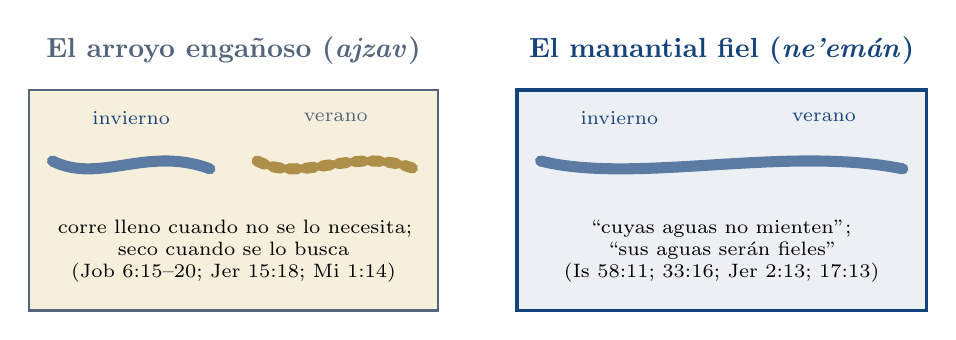
\begin{tikzpicture}[font=\small]
 % Arroyo engañoso
 \begin{scope}
  \node[font=\bfseries,text=gris] at (2.6,3.3) {El arroyo engañoso (\emph{ajzav})};
  \fill[papiro] (0,0) rectangle (5.2,2.8);
  \draw[gris,line width=0.8pt] (0,0) rectangle (5.2,2.8);
  \node[font=\scriptsize,text=azul] at (1.3,2.45) {invierno};
  \draw[azul!70,line width=4pt,line cap=round] (0.3,1.9) .. controls (0.9,1.6) and (1.5,2.1) .. (2.3,1.8);
  \node[font=\scriptsize,text=gris] at (3.9,2.45) {verano};
  \draw[dorado!80!gris,line width=4pt,line cap=round,dash pattern=on 3pt off 3pt] (2.9,1.9) .. controls (3.5,1.6) and (4.1,2.1) .. (4.9,1.8);
  \node[text width=4.8cm,align=center,font=\scriptsize] at (2.6,0.75) {corre lleno cuando no se lo necesita;\\ seco cuando se lo busca\\ (Job 6:15--20; Jer 15:18; Mi 1:14)};
 \end{scope}
 % Manantial
 \begin{scope}[xshift=6.2cm]
  \node[font=\bfseries,text=azul] at (2.6,3.3) {El manantial fiel (\emph{ne'emán})};
  \fill[azul!8] (0,0) rectangle (5.2,2.8);
  \draw[azul,line width=1.2pt] (0,0) rectangle (5.2,2.8);
  \node[font=\scriptsize,text=azul] at (1.3,2.45) {invierno};
  \node[font=\scriptsize,text=azul] at (3.9,2.45) {verano};
  \draw[azul!70,line width=4pt,line cap=round] (0.3,1.9) .. controls (1.5,1.6) and (3.4,2.1) .. (4.9,1.8);
  \node[text width=4.8cm,align=center,font=\scriptsize] at (2.6,0.75) {``cuyas aguas no mienten'';\\ ``sus aguas serán fieles''\\ (Is 58:11; 33:16; Jer 2:13; 17:13)};
 \end{scope}
\end{tikzpicture}\par
{\footnotesize\color{gris}\textit{Figura 2.} El arroyo engañoso y el manantial fiel. \textit{Nota.} Elaboración propia.}
\end{center}

\subsection{La fuente de agua viva}
Jeremías da al \SENOR{} el nombre que corresponde a esta imagen. El pecado de Israel no consistió solo en buscar otra agua, sino en cambiar el manantial por depósitos que la pierden:

\begin{verso}{Jeremías 2:13}
Porque dos males ha hecho mi pueblo: me dejaron a mí, fuente de agua viva, y cavaron para sí cisternas, cisternas rotas que no retienen agua.
\end{verso}

El profeta vuelve sobre ello más adelante: ``Oh \SENOR, esperanza de Israel\ldots{} dejaron a \SENOR, manantial de aguas vivas'' (Jer 17:13). Y Jesús retoma la promesa cuando dice que ``el agua que yo le daré será en él una fuente de agua que salte para vida eterna'' (Jn 4:14).

La imagen condensa todo el atributo. Lo infiel no siempre es lo que nunca dio nada; con frecuencia es lo que dio en invierno y falta en verano. Preguntar por la fidelidad de Dios equivale a formular la pregunta de Jeremías: ¿será Dios como el \emph{wadi} en tiempo de sequía? La Escritura responde con el manantial, cuya agua está presente cuando se la busca.

\precision{la elección de esta imagen como eje del capítulo es una decisión de esta serie. Los textos (Job 6; Jer 15:18; Is 58:11; Mi 1:14) y el sentido de \emph{ajzav} como arroyo que se seca están en los diccionarios (BDB; HALOT).}

%===================================================================
\section{La fidelidad cantada}

\subsection{El Salmo 89: siete veces fidelidad, siete veces \emph{jésed}}
El Salmo 89 es el gran poema de la fidelidad de Dios, y se abre con un voto:

\hebverso{חַסְדֵי יְהוָה עוֹלָם אָשִׁירָה לְדֹר וָדֹר אוֹדִיעַ אֱמוּנָתְךָ בְּפִי}
\begin{verso}{Salmo 89:1–2 [89:2–3]}
Las misericordias de \SENOR{} cantaré perpetuamente; De generación en generación haré notoria tu fidelidad con mi boca. Porque dije: Para siempre será edificada misericordia; En los cielos mismos afirmarás tu verdad.
\end{verso}

El salmista cumple su voto mediante una repetición que el oyente hebreo podía percibir: en el salmo, \emph{emuná} aparece siete veces y \emph{jésed} otras siete.

\begin{center}\small\renewcommand{\arraystretch}{1.18}
\begin{tabular}{@{}L{1.6cm}L{6.4cm}L{6.4cm}@{}}
\toprule
\textbf{Verso} & \textbf{\emph{emuná}} (RVR1960) & \textbf{\emph{jésed}} (RVR1960) \\ \midrule
1 [2] & ``tu fidelidad'' & ``las misericordias'' \\
2 [3] & ``tu verdad'' & ``misericordia'' \\
5 [6] & ``tu verdad'' & --- \\
8 [9] & ``tu fidelidad te rodea'' & --- \\
14 [15] & --- & ``misericordia y verdad'' (\emph{emet}) \\
24 [25] & ``mi verdad'' & ``mi misericordia'' \\
28 [29] & (\emph{ne'emán}: ``mi pacto será firme'') & ``mi misericordia'' \\
33 [34] & ``ni falsearé mi verdad'' & ``no quitaré\ldots{} mi misericordia'' \\
49 [50] & ``que juraste a David por tu verdad'' & ``tus antiguas misericordias'' \\
\bottomrule
\end{tabular}\par
{\footnotesize\color{gris}\textit{Tabla 5.} \emph{Emuná} y \emph{jésed} en el Salmo 89. \textit{Nota.} Conteo propio con la BHS; numeración española [hebrea]. La RVR1960 traduce \emph{emuná} ``fidelidad'' dos veces y ``verdad'' cinco.}
\end{center}

El dato revela cómo opera la traducción: quien lee la RVR1960 encuentra ``fidelidad'' solo dos veces, mientras que el hebreo repite la palabra siete. Además, ambas palabras aparecen juntas en el primer verso y en el último uso (v. 49), de modo que la pareja \emph{jésed} y \emph{emuná} enmarca todo el salmo.

\subsection{La promesa a David y su crisis}
En el centro del salmo está la promesa que Natán dio a David (2~S 7:12--16), ahora cantada como juramento:

\begin{verso}{Salmo 89:30–35 [89:31–36]}
Si dejaren sus hijos mi ley, Y no anduvieren en mis juicios, Si profanaren mis estatutos, Y no guardaren mis mandamientos, Entonces castigaré con vara su rebelión, Y con azotes sus iniquidades. Mas no quitaré de él mi misericordia, Ni falsearé mi verdad. No olvidaré mi pacto, Ni mudaré lo que ha salido de mis labios. Una vez he jurado por mi santidad, Y no mentiré a David.
\end{verso}

\begin{filologia}{Sal 89:33--35}
\heb{וְלֹא־אֲשַׁקֵּר בֶּאֱמוּנָתִי} & \heb{שׁקר} & ``y no mentiré en mi fidelidad'': el verbo de \emph{shéqer}, la mentira (cap. 13). RVR1960: ``ni falsearé mi verdad''. \\
\heb{וּמוֹצָא שְׂפָתַי לֹא אֲשַׁנֶּה} & \heb{שׁנה} & ``y lo que salió de mis labios no lo cambiaré''. \\
\heb{אִם־לְדָוִד אֲכַזֵּב} & \heb{כזב} & ``si a David miento'': fórmula de juramento. El verbo de \emph{ajzav}: Dios no será un arroyo engañoso para David. \\
\end{filologia}

Pink recurre a estos versos para mostrar que la disciplina no contradice la fidelidad: ``El castigo, no sólo es reconciliable con la tierna misericordia de Dios, sino que es el efecto y la expresión de la misma'' (Pink, 2020, cap. 10, p. 57). Dios promete la vara y, al mismo tiempo, promete no retirar la \emph{jésed}; ambas promesas son expresión de su fidelidad.

El salmo, sin embargo, no se detiene en el juramento. A partir del v. 38 el tono cambia bruscamente:

\begin{verso}{Salmo 89:38–39, 46, 49 [89:39–40, 47, 50]}
Mas tú desechaste y menospreciaste a tu ungido, Y te has airado con él. Rompiste el pacto de tu siervo; Has profanado su corona hasta la tierra\ldots{} ¿Hasta cuándo, oh \SENOR? ¿Te esconderás para siempre?\ldots{} Señor, ¿dónde están tus antiguas misericordias, Que juraste a David por tu verdad?
\end{verso}

\begin{center}
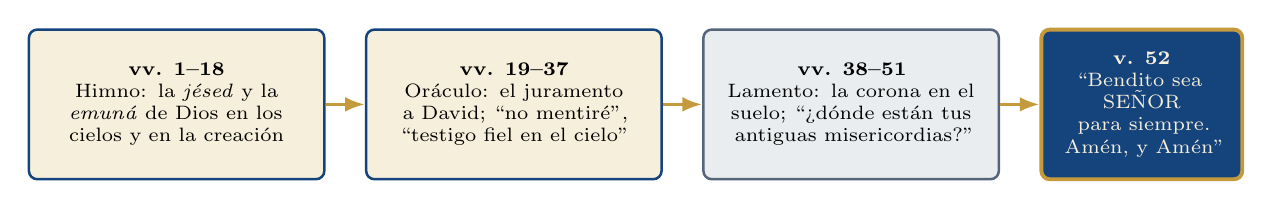
\begin{tikzpicture}[font=\scriptsize]
 \node[draw=azul,line width=0.9pt,fill=papiro,rounded corners=3pt,text width=3.4cm,align=center,inner sep=5pt,minimum height=1.9cm] (a) {\textbf{vv. 1--18}\\ Himno: la \emph{jésed} y la \emph{emuná} de Dios en los cielos y en la creación};
 \node[draw=azul,line width=0.9pt,fill=papiro,rounded corners=3pt,text width=3.4cm,align=center,inner sep=5pt,minimum height=1.9cm,right=0.5cm of a] (b) {\textbf{vv. 19--37}\\ Oráculo: el juramento a David; ``no mentiré'', ``testigo fiel en el cielo''};
 \node[draw=gris,line width=0.9pt,fill=gris!12,rounded corners=3pt,text width=3.4cm,align=center,inner sep=5pt,minimum height=1.9cm,right=0.5cm of b] (c) {\textbf{vv. 38--51}\\ Lamento: la corona en el suelo; ``¿dónde están tus antiguas misericordias?''};
 \node[draw=dorado,line width=1.4pt,fill=azul,text=papiro,rounded corners=3pt,text width=2.2cm,align=center,inner sep=5pt,minimum height=1.9cm,right=0.5cm of c] (d) {\textbf{v. 52}\\ ``Bendito sea \SENOR{} para siempre. Amén, y Amén''};
 \draw[-{Latex[length=2.5mm]},dorado,line width=1.2pt] (a)--(b);
 \draw[-{Latex[length=2.5mm]},dorado,line width=1.2pt] (b)--(c);
 \draw[-{Latex[length=2.5mm]},dorado,line width=1.2pt] (c)--(d);
\end{tikzpicture}\par
{\footnotesize\color{gris}\textit{Figura 3.} Las tres partes del Salmo 89 y su doxología. \textit{Nota.} Elaboración propia; numeración española.}
\end{center}

El poeta canta la fidelidad sobre las ruinas de la monarquía davídica. No niega el juramento, sino que se lo recuerda a Dios: es la fe que reclama la fidelidad precisamente cuando no se la ve, la misma que Pink describe: ``Hay épocas en la vida de todas las personas cuando no es fácil, ni siquiera para los cristianos, creer que Dios es fiel'' (Pink, 2020, cap. 10, p. 54). El v. 52 cierra el tercer libro de los Salmos con un ``Amén, y Amén'', palabra de la misma raíz que la fidelidad. La respuesta a la pregunta del v. 49 llegará en Isaías 55:3 y en Pablo (sección~\ref{sec:davidfiel}).

\precision{la división del salmo en himno, oráculo y lamento es la habitual en los comentarios; la ocasión histórica del lamento (la caída de un rey davídico, probablemente en el destierro) se discute. El v. 52 es la doxología que cierra el Libro III del Salterio (Sal 73--89), no una parte original del poema.}

\subsection{“Grande es tu fidelidad”: en el centro del acróstico}
Lamentaciones, escrito sobre las ruinas de Jerusalén, sitúa en su centro la frase más conocida sobre la fidelidad de Dios:

\hebverso{חַסְדֵי יְהוָה כִּי לֹא־תָמְנוּ כִּי לֹא־כָלוּ רַחֲמָיו \\ חֲדָשִׁים לַבְּקָרִים רַבָּה אֱמוּנָתֶךָ}
\begin{verso}{Lamentaciones 3:21–24}
Esto recapacitaré en mi corazón, por lo tanto esperaré. Por la misericordia de \SENOR{} no hemos sido consumidos, porque nunca decayeron sus misericordias. Nuevas son cada mañana; grande es tu fidelidad. Mi porción es \SENOR, dijo mi alma; por tanto, en él esperaré.
\end{verso}

El capítulo 14 estudió estos versos desde la misericordia; aquí interesa su última palabra: \heb{רַבָּה אֱמוּנָתֶךָ} (\emph{rabbá emunatéja}), ``grande es tu fidelidad''. Esa fidelidad se renueva ``cada mañana'', como el maná. El poeta no la deduce de las circunstancias, que son de ruina, sino de la memoria: ``esto recapacitaré en mi corazón'' (\heb{זֹאת אָשִׁיב אֶל־לִבִּי}, ``esto haré volver a mi corazón''). Su respuesta es esperar (\heb{אוֹחִיל}), y lo dice dos veces (vv. 21, 24).

\precision{(textual) el texto griego de la Septuaginta usado en esta serie no contiene Lam 3:22--24, sino que salta del v. 21 al 25 (conviene cotejarlo en la edición de Rahlfs-Hanhart). Los versos están en el texto masorético, que la RVR1960 sigue.}

\subsection{La letra que falta: \emph{nun} en el Salmo 145}
El Salmo 145 es un acróstico en el que cada verso comienza con una letra del alfabeto hebreo. En el texto masorético, sin embargo, falta la letra \emph{nun} (\heb{נ}), que debería ir entre el v. 13 (\emph{mem}) y el v. 14 (\emph{sámej}), y por eso la RVR1960, que sigue ese texto, no tiene el verso. Otros testigos sí lo conservan:

\begin{center}\small\renewcommand{\arraystretch}{1.25}
\begin{tabular}{@{}L{3.6cm}L{10.8cm}@{}}
\toprule
\textbf{Testigo} & \textbf{El verso de \emph{nun}} \\ \midrule
Texto masorético & no lo tiene; el acróstico pasa de \emph{mem} a \emph{sámej} \\
11QPs\textsuperscript{a} (Qumrán) & \heb{נאמן אלוהים בדבריו וחסיד בכול מעשיו}: ``Fiel es Dios en sus palabras, y bondadoso en todas sus obras'' \\
Septuaginta (Sal 144:13a) & \grc{πιστὸς κύριος ἐν τοῖς λόγοις αὐτοῦ καὶ ὅσιος ἐν πᾶσι τοῖς ἔργοις αὐτοῦ}: ``Fiel es el Señor en sus palabras, y santo en todas sus obras'' \\
\bottomrule
\end{tabular}\par
{\footnotesize\color{gris}\textit{Tabla 6.} El verso de \emph{nun} del Salmo 145. \textit{Nota.} 11QPs\textsuperscript{a} según Sanders (1965); LXX según Rahlfs-Hanhart.}
\end{center}

El verso ausente comienza precisamente con \emph{ne'emán}: ``Fiel es Dios en sus palabras''. Y el que le sigue en el texto masorético emplea el verbo del texto ancla de este capítulo: ``Sostiene \SENOR{} a todos los que caen (\heb{הַנֹּפְלִים}, \emph{hanofelim}), y levanta a todos los oprimidos'' (Sal 145:14).

\precision{(textual) los estudiosos están divididos: unos piensan que el verso de \emph{nun} se perdió en la copia del texto masorético; otros, que fue añadido después para completar el acróstico. La RVR1960 sigue el texto masorético. El texto de 11QPs\textsuperscript{a} se cita desde Sanders (1965); conviene cotejarlo con las imágenes del rollo en la Leon Levy Dead Sea Scrolls Digital Library.}

El Talmud ya conocía el salmo sin \emph{nun} y se preguntó por la razón de esa ausencia. Su respuesta se estudia en la sección sobre el judaísmo.

%===================================================================
\section{Teología: el Dios que no puede negarse a sí mismo}

La teología de la fidelidad parte del Nombre que la revela. Moisés no presenta a Israel una cualidad que Dios posea ocasionalmente, sino lo que Dios es: ``Conoce, pues, que \SENOR{} tu Dios es Dios, Dios fiel, que guarda el pacto y la misericordia a los que le aman y guardan sus mandamientos, hasta mil generaciones'' (Dt 7:9). Si la fidelidad pertenece a su ser, Dios no podría dejar de ser fiel sin dejar de ser Dios. Pablo lo afirma con una frase que sorprende justamente porque toma en serio la infidelidad humana: ``Si fuéremos infieles, él permanece fiel; él no puede negarse a sí mismo'' (2~Ti 2:13). La fidelidad de Dios no depende de la respuesta del hombre, porque su raíz no está en el hombre, sino en Dios mismo. Pink lo observa con precisión: ``esta cualidad es esencial para su Ser; sin ella no sería Dios. Para Dios, ser infiel, sería actuar en contra de su naturaleza, lo cual sería imposible'' (Pink, 2020, cap. 10, p. 53); de ahí que ``él nunca olvida, nunca falla, nunca vacila, nunca falta a su Palabra'' (Pink, 2020, cap. 10, pp. 53--54). Es, formulada en negativo, la misma definición de esta serie.

\subsection{La fidelidad en la oscuridad}
Que Dios es fiel se cree con facilidad en la teoría y con dificultad en la prueba. Pink lo advierte: ``una cosa es aceptar la fidelidad de Dios como una verdad divina y otra muy distinta es actuar de acuerdo con ella'' (Pink, 2020, cap. 10, p. 54). Isaías se dirige precisamente al creyente que no ve:

\begin{verso}{Isaías 50:10}
¿Quién hay entre vosotros que teme a \SENOR, y oye la voz de su siervo? El que anda en tinieblas y carece de luz, confíe en el nombre de \SENOR, y apóyese en su Dios.
\end{verso}

``Apóyese'' traduce \heb{וְיִשָּׁעֵן} (\emph{veyisha'én}), ``que se recueste'': quien no ve el camino descansa su peso en Aquel que no falla. El profeta no promete luz inmediata, sino un apoyo firme en medio de la oscuridad. Jesús dirá algo semejante a Pedro: ``Lo que yo hago, tú no lo comprendes ahora; mas lo entenderás después'' (Jn 13:7). La demora, por tanto, no es indiferencia, sino una espera de Dios mismo: ``\SENOR{} esperará para tener piedad de vosotros'' (Is 30:18). La fidelidad de Dios incluye también sus tiempos.

\subsection{La fidelidad en tres obras}
La Escritura muestra esa fidelidad en tres obras que abarcan toda la vida del pueblo de Dios. La primera es preservar. Pablo escribe a los corintios que Cristo ``os confirmará hasta el fin, para que seáis irreprensibles en el día de nuestro Señor Jesucristo. Fiel es Dios, por el cual fuisteis llamados a la comunión con su Hijo'' (1~Co 1:8--9). La perseverancia del creyente no descansa, en palabras de Pink, ``en la fuerza de sus resoluciones'', sino ``en la veracidad de Aquel que no puede mentir'' (Pink, 2020, cap. 10, p. 56).

La segunda obra es disciplinar, y es la que más cuesta reconocer como fidelidad. El salmista, sin embargo, la reconoce: ``Conozco, oh \SENOR, que tus juicios son justos, y que conforme a tu fidelidad me afligiste'' (Sal 119:75). Lejos de contradecir la fidelidad, la aflicción nace de ella, porque Dios no abandona a los suyos a su extravío. Por eso, como observa Pink, Dios ``es tan fiel cuando retiene algo como cuando da algo'' (Pink, 2020, cap. 10, pp. 56--57).

La tercera obra es glorificar: el Dios que comenzó la obra la llevará a término. ``Fiel es el que os llama, el cual también lo hará'' (1~Ts 5:24). Pablo encadena el llamado con la gloria final sin dejar un eslabón suelto: ``a los que llamó, a éstos también justificó; y a los que justificó, a éstos también glorificó'' (Ro 8:30). Preservar, disciplinar y glorificar son, así, tres momentos de una misma fidelidad.

\subsection{Descansar en el fiel Creador}
De esa certeza nace una manera de vivir. La fidelidad de Dios, escribe Pink, ``nos preservará de la preocupación'', ``refrenará nuestros sollozos'' y ``engendrará una confianza cada vez mayor en Dios'' (Pink, 2020, cap. 10, pp. 57--58). Pedro convierte esa certeza en exhortación para los que sufren: ``De modo que los que padecen según la voluntad de Dios, encomienden sus almas al fiel Creador, y hagan el bien'' (1~P 4:19). Encomendar el alma significa entregar en depósito lo más valioso a quien no puede fallar; hacer el bien es la respuesta de quien ya no necesita defenderse a sí mismo.

\precision{Pink (2020, cap. 10) presenta también a Faraón, Coré y Acán como ejemplos de fidelidad en el juicio, y cita un himno de William Cowper (\emph{God moves in a mysterious way}). El capítulo 13 estudió lo que corresponde a la veracidad (Nm 23:19 y las promesas a Abraham y por Isaías); aquí se estudia lo que es propio de la fidelidad.}

%===================================================================
\section{Un encuentro en la historia de Israel: Salomón en la dedicación del templo}

Unos cuatro siglos después de Josué, Salomón concluyó el templo que David había querido edificar. Dios había dicho a David que no lo construiría él, sino su hijo, y le había prometido una casa, es decir, una dinastía (2~S 7:12--16). En la dedicación, con el arca ya en el lugar santísimo y la nube llenando la casa (1~R 8:10--11), Salomón se vuelve hacia el pueblo y lo bendice:

\hebverso{בָּרוּךְ יְהוָה אֱלֹהֵי יִשְׂרָאֵל אֲשֶׁר דִּבֶּר בְּפִיו אֵת דָּוִד אָבִי וּבְיָדוֹ מִלֵּא}
\begin{verso}{1 Reyes 8:15, 20}
Y dijo: Bendito sea \SENOR, Dios de Israel, que habló a David mi padre lo que con su mano ha cumplido, diciendo\ldots{} Y \SENOR{} ha cumplido su palabra que había dicho; porque yo me he levantado en lugar de David mi padre, y me he sentado en el trono de Israel, como \SENOR{} había dicho, y he edificado la casa al nombre de \SENOR{} Dios de Israel.
\end{verso}

\begin{filologia}{1 R 8:15--26}
\heb{דִּבֶּר בְּפִיו} \ldots{} \heb{וּבְיָדוֹ מִלֵּא} & \heb{מלא} & ``habló con su boca\ldots{} y con su mano llenó'' (v. 15; también v. 24). La boca promete; la mano llena la promesa. \\
\heb{וַיָּקֶם יְהוָה אֶת־דְּבָרוֹ} \ldots{} \heb{וָאָקֻם} & \heb{קום} & ``y levantó el \SENOR{} su palabra\ldots{} y yo me levanté'' (v. 20). Salomón mismo es la palabra puesta en pie. \\
\heb{יֵאָמֶן נָא דְּבָרֶיךָ} & \heb{אמן} & ``sea afirmada, te ruego, tu palabra'' (v. 26): nifal de \emph{amán}, la raíz de \emph{ne'emán}. RVR1960: ``cúmplase la palabra''. \\
\heb{לֹא־נָפַל דָּבָר אֶחָד} & \heb{נפל} & ``no cayó una sola palabra'' (v. 56): la frase de Jos 21:45 y 23:14. \\
\end{filologia}

La oración que sigue se construye sobre la fidelidad. Salomón comienza confesando lo que Dios ya hizo y, desde ahí, pide lo que todavía falta:

\begin{verso}{1 Reyes 8:23–26}
\SENOR{} Dios de Israel, no hay Dios como tú, ni arriba en los cielos ni abajo en la tierra, que guardas el pacto y la misericordia a tus siervos, los que andan delante de ti con todo su corazón; que has cumplido a tu siervo David mi padre lo que le prometiste; lo dijiste con tu boca, y con tu mano lo has cumplido, como sucede en este día. Ahora, pues, \SENOR{} Dios de Israel, cumple a tu siervo David mi padre lo que le prometiste\ldots{} Ahora, pues, oh \SENOR{} Dios de Israel, cúmplase la palabra que dijiste a tu siervo David mi padre.
\end{verso}

La fórmula ``que guardas el pacto y la misericordia'' reproduce Dt 7:9 casi palabra por palabra: Salomón ora invocando el Nombre del Dios fiel. Su oración sigue la lógica de toda oración bíblica de confianza: \emph{lo que ya cumpliste es la garantía de lo que te pido que cumplas}. Así había orado también David: ``confirma para siempre la palabra que has hablado sobre tu siervo\ldots{} y haz conforme a lo que has dicho'' (2~S 7:25).

Al terminar, Salomón bendice al pueblo con las palabras de Josué:

\begin{verso}{1 Reyes 8:56–57}
Bendito sea \SENOR, que ha dado paz a su pueblo Israel, conforme a todo lo que él había dicho; ninguna palabra de todas sus promesas que expresó por Moisés su siervo, ha faltado. Esté con nosotros \SENOR{} nuestro Dios, como estuvo con nuestros padres, y no nos desampare ni nos deje.
\end{verso}

``Reposo'' (\heb{מְנוּחָה}) y ``ninguna palabra ha caído'': con el templo se cumple el reposo que Josué había iniciado (Jos 21:44) y que Dt 12:9--10 anunciaba. Dos generaciones de la historia de Israel, la de Josué y la de Salomón, suscriben la misma frase.

El relato, con todo, no termina en la fiesta. En la segunda aparición, Dios advierte a Salomón: ``si obstinadamente os apartareis de mí\ldots{} yo cortaré a Israel de sobre la faz de la tierra\ldots{} y esta casa\ldots{} yo la echaré de delante de mí'' (1~R 9:6--7). Resuena otra vez Jos 23:15, con su palabra buena y su palabra mala. Casi cuatro siglos más tarde, el templo fue quemado (2~R 25:9); y aun entonces la fidelidad siguió hablando: ``Cuando en Babilonia se cumplan los setenta años, yo os visitaré, y despertaré sobre vosotros mi buena palabra'' (Jer 29:10). Por eso el libro de Esdras se abre con el decreto de Ciro, promulgado ``para que se cumpliese la palabra de \SENOR{} por boca de Jeremías'' (Esd 1:1).

\precision{``Despertaré\ldots{} mi buena palabra'' (Jer 29:10) traduce \heb{וַהֲקִמֹתִי עֲלֵיכֶם אֶת־דְּבָרִי הַטּוֹב}, ``levantaré sobre vosotros mi palabra buena'', con el mismo verbo de 1~R 8:20 y la misma ``palabra buena'' de Jos 21:45. La cadena Josué--Salomón--Jeremías es una lectura propia de esta serie, apoyada en ese vocabulario común.}

%===================================================================
\section{La fidelidad en el judaísmo}

\subsection{“Dios, Rey fiel”: el sentido del amén}
El Talmud de Babilonia se pregunta qué significa la palabra con que el pueblo responde a cada bendición:

\hebverso{מַאי אָמֵן אָמַר רַבִּי חֲנִינָא אֵל מֶלֶךְ נֶאֱמָן}

``¿Qué es \emph{amén}? Dijo Rabí Janiná: \emph{El Mélej Ne'emán}'', ``Dios, Rey fiel'' (\emph{Shabat} 119b). Las tres palabras comienzan con las tres letras de \heb{אָמֵן}, álef, mem y nun, de modo que quien dice ``amén'' confiesa que el que bendijo es un Rey que cumple.

\precision{interpretación rabínica (Talmud de Babilonia, edición William Davidson en Sefaria). La lectura de \emph{amén} como sigla es un recurso homilético, no una etimología: \emph{amén} procede de la raíz \emph{amán} (capítulo 13). Con todo, la sigla expresa bien lo que la raíz significa.}

\subsection{“El Dios fiel, que dice y hace”}
Ya en el siglo I se leía en la sinagoga cada sábado, después de la Torá, una sección de los Profetas; fue ``después de la lectura de la ley y de los profetas'' cuando Pablo recibió la invitación a hablar en Antioquía de Pisidia (Hch 13:15). Esa lectura se llama \emph{haftará}, y el tratado \emph{Masejet Soferim} (cap. 13) conserva la bendición que se pronuncia tras ella. En el sidur sefardí reza así:

\hebverso{הָאֵל הַנֶּאֱמָן הָאוֹמֵר וְעוֹשֶׂה הַמְדַבֵּר וּמְקַיֵּם שֶׁכָּל דְּבָרָיו אֱמֶת וָצֶדֶק \\ נֶאֱמָן אַתָּה הוּא יְהוָה אֱלֹהֵינוּ וְנֶאֱמָנִים דְּבָרֶיךָ \\ וְדָבָר אֶחָד מִדְּבָרֶיךָ אָחוֹר לֹא יָשׁוּב רֵיקָם כִּי אֵל מֶלֶךְ נֶאֱמָן וְרַחֲמָן אָתָּה}

\begin{quote}\itshape
\ldots{}el Dios fiel, que dice y hace, que habla y cumple, porque todas sus palabras son verdad y justicia. Fiel eres tú, \SENOR{} nuestro Dios, y fieles son tus palabras, y ni una sola de tus palabras vuelve atrás vacía, porque tú eres Dios, Rey fiel y misericordioso. Bendito eres tú, \SENOR, el Dios fiel en todas sus palabras.\par\hfill{\upshape\small\bfseries\textcolor{azul}{(Bendición después de la \emph{haftará}; \emph{Masejet Soferim} 13)}}
\end{quote}

La bendición ofrece una definición litúrgica del atributo, tejida con textos bíblicos. ``El Dios fiel'' procede de Dt 7:9. ``Que habla y cumple'' (\heb{הַמְדַבֵּר וּמְקַיֵּם}, ``que habla y pone en pie'') emplea el verbo \emph{qum} de 1~R 8:20. ``Ni una sola de tus palabras vuelve atrás vacía'' recoge Is 55:11: ``así será mi palabra que sale de mi boca; no volverá a mí vacía'' (\heb{לֹא־יָשׁוּב אֵלַי רֵיקָם}). El cierre, por último, ``Dios, Rey fiel'', es la sigla del amén de \emph{Shabat} 119b.

\precision{texto según el \emph{Sidur Sefard} (servicio de la mañana del sábado) y \emph{Masejet Soferim} 13 en Sefaria; las variantes entre sidurim son menores. Sobre la historia de la lectura de los Profetas y sus bendiciones, véase Elbogen (1993). No es casual que la bendición se pronuncie justo después de los Profetas: en ellos se anuncian las promesas que Dios cumplirá.}

\subsection{La \emph{Amidá}: fiel a los que duermen en el polvo}
La segunda bendición de la \emph{Amidá}, la oración que el judío recita tres veces al día, alaba el poder de Dios (capítulo 9), y en ella aparecen dos frases sobre la fidelidad:

\hebverso{וּמְקַיֵּם אֱמוּנָתוֹ לִישֵׁנֵי עָפָר \\ וְנֶאֱמָן אַתָּה לְהַחֲיוֹת מֵתִים}

``\ldots{}y cumple su fidelidad a los que duermen en el polvo'' y ``fiel eres tú para dar vida a los muertos''. La primera toma la expresión de Dn 12:2: ``muchos de los que duermen en el polvo de la tierra serán despertados''. La fidelidad de Dios, entonces, no termina en la tumba: la promesa hecha a los padres se cumplirá también en los muertos. En la misma bendición, Dios es \heb{סוֹמֵךְ נוֹפְלִים}, ``el que sostiene a los que caen'', con palabras de Sal 145:14.

\precision{texto según el \emph{Sidur Ashkenaz} en Sefaria. La \emph{Amidá} se fijó en su forma básica después de la destrucción del segundo templo, y la redacción exacta de algunas frases varió durante siglos (Elbogen, 1993). La conexión entre esta fidelidad ``a los que duermen'' y la resurrección es explícita en la bendición misma.}

\subsection{\emph{Modé aní}: la fidelidad cada mañana}
La primera oración del día, que se dice al despertar, todavía en la cama, concluye con las palabras de Lamentaciones:

\hebverso{מוֹדֶה אֲנִי לְפָנֶיךָ מֶלֶךְ חַי וְקַיָּם \\ שֶׁהֶחֱזַרְתָּ בִּי נִשְׁמָתִי בְּחֶמְלָה רַבָּה אֱמוּנָתֶךָ}

``Te doy gracias, Rey vivo y permanente, porque me devolviste el alma con compasión: grande es tu fidelidad''. La oración lee Lam 3:23 al pie de la letra, pues las misericordias ``nuevas cada mañana'' son el aliento que vuelve al despertar.

\precision{texto según el \emph{Sidur Ashkenaz} en Sefaria. \emph{Modé aní} es una oración tardía, que aparece por primera vez en el \emph{Séder haYom} de Moshé ben Majir (s.~XVI). La idea de que el alma se entrega a Dios al dormir y se recibe de vuelta al despertar es, en cambio, más antigua en la tradición judía.}

\subsection{La letra que falta y el que sostiene a los que caen}
El Talmud conocía el Salmo 145 sin el verso de \emph{nun} y propuso una explicación:

\begin{quote}\itshape
Dijo Rabí Yojanán: ¿Por qué no se dice \emph{nun} en el \emph{Ashré} (Sal 145)? Porque en ella está la caída de [los enemigos de] Israel, como está escrito: ``Cayó la virgen de Israel, y no podrá levantarse ya más'' (Am 5:2)\ldots{} Dijo Rav Najmán bar Yitsjak: Aun así, David volvió a sostenerlos por el Espíritu Santo, como está dicho: ``Sostiene el \SENOR{} a todos los que caen'' (Sal 145:14).\par\hfill{\upshape\small\bfseries\textcolor{azul}{(\emph{Berajot} 4b)}}
\end{quote}

\hebverso{סוֹמֵךְ יְהוָה לְכָל־הַנֹּפְלִים}

Am 5:2 comienza con \heb{נָפְלָה} (\emph{nafelá}), ``cayó''. Según el Talmud, David no quiso iniciar un verso con la letra de la caída; pero en el verso siguiente, que empieza con \emph{sámej}, el \SENOR{} sostiene a ``los que caen''. Se trata del mismo verbo de Jos 21:45: la palabra de Dios no cae, y Dios levanta a los que caen.

\precision{interpretación rabínica; ``los enemigos de Israel'' es un eufemismo del Talmud para no decir ``la caída de Israel''. La lectura que une \emph{Berajot} 4b con el verbo de Jos 21:45 es propia de esta serie. El verso de \emph{nun} que conservan Qumrán y la LXX (``Fiel es Dios en sus palabras'') no forma parte del texto que comentaba el Talmud.}

\subsection{“Aunque demore su recompensa”}
El Sifré, un midrash antiguo sobre Deuteronomio, comenta el título \emph{El emuná} de Dt 32:4 con una frase atrevida:

\hebverso{אֵל אֱמוּנָה שֶׁהֶאֱמִין בָּעוֹלָם וּבְרָאוֹ}

``Dios de fidelidad: que tuvo confianza en el mundo y lo creó'' (\emph{Sifré Devarim} 307). El midrash juega con la raíz, pues Dios es fiel y, a la vez, ``confió'' al crear; y añade que Dios retribuye a cada uno con exactitud, en este mundo o en el venidero. Rashi resume el pasaje con una frase que toca el punto más difícil de la fidelidad, la demora:

\begin{quote}\itshape
Para pagar a los justos su justicia en el mundo venidero; y aunque demore su recompensa, al final hace firmes sus palabras.\par\hfill{\upshape\small\bfseries\textcolor{azul}{(Rashi a Dt 32:4)}}
\end{quote}

``Al final hace firmes sus palabras'' traduce \heb{סוֹפוֹ לְאַמֵּן אֶת דְּבָרָיו}, y el verbo es, una vez más, \emph{amán}. La fidelidad abarca también el tiempo de espera.

\precision{interpretaciones rabínicas, según Sefaria (\emph{Sifré Devarim} 307; Rashi a Dt 32:4).}

\subsection{Qumrán: la espera y la fidelidad}
El \emph{Pésher de Habacuc} (1QpHab), uno de los primeros rollos hallados en Qumrán, comenta Hab 2:3--4 desde la experiencia de una comunidad que esperaba el fin y constataba que no llegaba. A propósito de ``aunque la visión tardará aún por un tiempo\ldots{} aunque tardare, espéralo'' (Hab 2:3), explica que ``el tiempo final se prolongará y excederá todo lo que dijeron los profetas, porque los misterios de Dios son asombrosos'', y que el texto alude a ``los hombres de verdad que cumplen la Ley, cuyas manos no se aflojarán en el servicio de la verdad cuando el tiempo final se prolongue'' (1QpHab VII 5--14). En cuanto a ``el justo por su fe vivirá'' (Hab 2:4), lo refiere a quienes cumplen la Ley en la casa de Judá, a los que Dios librará del juicio ``por su sufrimiento y por su fidelidad al Maestro de Justicia'' (1QpHab VIII 1--3).

\precision{traducción propia desde la versión de Vermes (2004); cf. García Martínez (1992). El término traducido ``fidelidad'' es la \emph{emuná} de Hab 2:4. Que Qumrán y Pablo comenten el mismo versículo, con lecturas distintas, muestra que Hab 2:4 era un texto clave del judaísmo del siglo I.}

%===================================================================
\section{La fidelidad en Cristo, leída con Pablo}

\subsection{“No que la palabra de Dios haya fallado”}
En Romanos 9--11 Pablo enfrenta la pregunta más dura que un judío de su tiempo podía plantear sobre la fidelidad de Dios: si el Mesías vino y la mayor parte de Israel no lo recibió, ¿falló la promesa? Tras enumerar los privilegios de Israel, ``la adopción, la gloria, el pacto, la promulgación de la ley, el culto y las promesas'' (Ro 9:4), responde:

\begin{verso}{Romanos 9:6}
No que la palabra de Dios haya fallado; porque no todos los que descienden de Israel son israelitas.
\end{verso}

\begin{filologia}{Ro 9:6}
\grc{οὐχ οἷον δὲ ὅτι ἐκπέπτωκεν} & \grc{ἐκπίπτω} & ``no es que haya caído'': perfecto de \grc{ἐκπίπτω}, ``caer fuera, caer al suelo''. La RVR1960 traduce ``haya fallado''. \\
\grc{ὁ λόγος τοῦ θεοῦ} & \grc{λόγος} & ``la palabra de Dios'': las promesas a los padres (Ro 9:4, 8--9). \\
\grc{οὐ διέπεσεν} (Jos 21:45 LXX) & \grc{πίπτω} & la Septuaginta de Josué usa la misma imagen: la palabra ``no cayó''. \\
\end{filologia}

Pablo formula la pregunta del Salmo 89:49 y responde con la certeza de Josué: la palabra no cayó. Los capítulos 9--11 desarrollan esa respuesta hasta llegar a ``¿Ha desechado Dios a su pueblo? En ninguna manera'' (Ro 11:1) y a ``irrevocables son los dones y el llamamiento de Dios'' (Ro 11:29; capítulo 8). Ya en Ro 3:3 había planteado la misma cuestión: ``¿Su incredulidad habrá hecho nula la fidelidad de Dios?'' (\grc{τὴν πίστιν τοῦ θεοῦ}; capítulo 13).

\precision{la relación verbal entre Ro 9:6 (\grc{ἐκπέπτωκεν}) y Jos 21:45 LXX (\grc{οὐ διέπεσεν}) es una lectura propia de esta serie: los verbos pertenecen a la misma familia y la imagen es la misma, pero Pablo no cita Josué. Que la pregunta de Ro 9--11 sea la fidelidad de Dios a Israel es la lectura común de los comentarios (Moo, 1996; Wright, 2013).}

\subsection{“Fiel es Dios”: una fórmula de Pablo}
Pablo convierte el título de Dt 7:9 en una fórmula que repite a lo largo de sus cartas, y siempre en el mismo punto del argumento: cuando la iglesia mira al futuro y teme no llegar.

\begin{center}\small\renewcommand{\arraystretch}{1.22}
\begin{tabular}{@{}L{2.2cm}L{5.4cm}L{6.8cm}@{}}
\toprule
\textbf{Texto} & \textbf{Griego} & \textbf{Lo que Dios hará por ser fiel} \\ \midrule
1~Co 1:9 & \grc{πιστὸς ὁ θεός} & confirmar a los creyentes ``hasta el fin'' (v. 8) en la comunión con su Hijo \\
1~Co 10:13 & \grc{πιστὸς δὲ ὁ θεός} & no permitir la prueba más allá de lo que se puede resistir; dar la salida \\
2~Co 1:18 & \grc{πιστὸς δὲ ὁ θεός} & que su palabra no sea ``Sí y No'' (capítulo 13) \\
1~Ts 5:24 & \grc{πιστὸς ὁ καλῶν ὑμᾶς} & santificar por completo y guardar hasta la venida de Cristo \\
2~Ts 3:3 & \grc{πιστὸς δέ ἐστιν ὁ κύριος} & afirmar y guardar del mal \\
2~Ti 2:13 & \grc{ἐκεῖνος πιστὸς μένει} & permanecer fiel aunque seamos infieles \\
\bottomrule
\end{tabular}\par
{\footnotesize\color{gris}\textit{Tabla 7.} La fórmula ``Fiel es Dios'' en las cartas de Pablo. \textit{Nota.} Texto griego NA28.}
\end{center}

\precision{la autoría paulina de 2 Tesalonicenses y 2 Timoteo se discute. La fórmula, sin embargo, está en cartas indiscutidas (1 Corintios, 2 Corintios, 1 Tesalonicenses), y la idea de 2~Ti 2:13 se encuentra ya en Ro 3:3--4.}

\subsection{Llamados a la comunión del Hijo}
\begin{verso}{1 Corintios 1:8–9}
el cual también os confirmará hasta el fin, para que seáis irreprensibles en el día de nuestro Señor Jesucristo. Fiel es Dios, por el cual fuisteis llamados a la comunión con su Hijo Jesucristo nuestro Señor.
\end{verso}

\begin{filologia}{1 Co 1:8--9}
\grc{βεβαιώσει ὑμᾶς ἕως τέλους} & \grc{βεβαιόω} & ``os hará firmes hasta el fin'': el verbo griego de la firmeza, cercano a \emph{amán}. \\
\grc{πιστὸς ὁ θεός} & \grc{πιστός} & ``fiel es Dios'': sin verbo, como una confesión. LXX Dt 7:9: \grc{θεὸς πιστός}. \\
\grc{εἰς κοινωνίαν τοῦ υἱοῦ αὐτοῦ} & \grc{κοινωνία} & ``a la comunión de su Hijo'': participar en él, ser de él. \\
\end{filologia}

Pablo se dirige aquí a la iglesia más problemática de sus cartas, marcada por divisiones, inmoralidad, pleitos y desorden en la Cena. Antes de corregir, sin embargo, establece el fundamento: los corintios llegarán al día de Cristo no por su propia firmeza, sino porque Dios es fiel. Pink subraya el mismo punto: la confianza del apóstol ``no se basó en la fuerza de sus resoluciones o capacidad de perseverar, sino en la veracidad de Aquel que no puede mentir'' (Pink, 2020, cap. 10, p. 56).

\subsection{Fiel en la prueba: la roca que los seguía}
En 1 Corintios 10 Pablo relee la historia del desierto. Israel pasó el mar, comió el maná y ``bebían de la roca espiritual que los seguía, y la roca era Cristo'' (10:4); pero cayó en idolatría, fornicación y murmuración, y ``cayeron en un día veintitrés mil'' (10:8). De ahí la advertencia: ``el que piensa estar firme, mire que no caiga'' (10:12). Y a continuación, el consuelo:

\begin{verso}{1 Corintios 10:13}
No os ha sobrevenido ninguna tentación que no sea humana; pero fiel es Dios, que no os dejará ser tentados más de lo que podéis resistir, sino que dará también juntamente con la tentación la salida, para que podáis soportar.
\end{verso}

El contraste es el que recorre todo este capítulo: el pueblo cae, Dios no. El Cántico de Moisés había llamado a Dios ``la Roca'' y \emph{El emuná}, título que la Septuaginta traduce \grc{θεὸς πιστός} (Dt 32:4); Pablo reúne ambas ideas en un mismo pasaje, donde Cristo es la roca que acompaña y Dios es fiel en la prueba.

\precision{es probable que Pablo tenga en mente Dt 32 en 1~Co 10, pues cita Dt 32:17 en 10:20 y alude a Dt 32:21 en 10:22 (Fee, 1987; Hays, 1989). El vínculo entre ``la roca'' de 10:4 y \grc{θεὸς πιστός} de 10:13 a través de Dt 32:4 es una lectura propia.}

\subsection{“El cual también lo hará”}
\begin{verso}{1 Tesalonicenses 5:23–24}
Y el mismo Dios de paz os santifique por completo; y todo vuestro ser, espíritu, alma y cuerpo, sea guardado irreprensible para la venida de nuestro Señor Jesucristo. Fiel es el que os llama, el cual también lo hará.
\end{verso}

En la frase \grc{πιστὸς ὁ καλῶν ὑμᾶς, ὃς καὶ ποιήσει} resuena, en boca de Pablo, la definición de esta serie: el que llama, cumple. La misma certeza reaparece en una carta indiscutida escrita desde la cárcel:

\begin{verso}{Filipenses 1:6}
estando persuadido de esto, que el que comenzó en vosotros la buena obra, la perfeccionará hasta el día de Jesucristo.
\end{verso}

``El que comenzó\ldots{} la perfeccionará'' (\grc{ὁ ἐναρξάμενος\ldots{} ἐπιτελέσει}): Dios no deja obras a medio hacer. Así creyó Abraham, ``plenamente convencido de que era también poderoso para hacer todo lo que había prometido'' (Ro 4:21; capítulo 9).

\subsection{“El justo por la fe vivirá”}
Habacuc se queja de que Dios tarda, y Dios le responde con una visión que ``no mentirá'' y que ``sin duda vendrá'' (Hab 2:3). En ese contexto de espera se encuentra la frase que Pablo sitúa al comienzo de Romanos:

\hebverso{וְצַדִּיק בֶּאֱמוּנָתוֹ יִחְיֶה}
\begin{verso}{Habacuc 2:4}
He aquí que aquel cuya alma no es recta, se enorgullece; mas el justo por su fe vivirá.
\end{verso}
\begin{verso}{Romanos 1:17}
Porque en el evangelio la justicia de Dios se revela por fe y para fe, como está escrito: Mas el justo por la fe vivirá.
\end{verso}

\begin{center}\small\renewcommand{\arraystretch}{1.25}
\begin{tabular}{@{}L{2.6cm}L{6.2cm}L{5.6cm}@{}}
\toprule
\textbf{Testigo} & \textbf{Texto} & \textbf{De quién es la fidelidad} \\ \midrule
Hab 2:4 TM & \heb{וְצַדִּיק בֶּאֱמוּנָתוֹ יִחְיֶה} & ``por \emph{su} \emph{emuná}'': la del justo, que se mantiene firme en la espera \\
Hab 2:4 LXX & \grc{ὁ δὲ δίκαιος ἐκ πίστεώς μου ζήσεται} & ``por \emph{mi} fidelidad'': la de Dios \\
1QpHab VIII 1--3 & ``por su fidelidad al Maestro de Justicia'' & la de la comunidad hacia su maestro \\
Ro 1:17; Gá 3:11 & \grc{ὁ δὲ δίκαιος ἐκ πίστεως ζήσεται} & sin pronombre: la fe del que cree, fundada en la fidelidad de Dios \\
He 10:38 & \grc{ὁ δὲ δίκαιός μου ἐκ πίστεως ζήσεται} & ``mi justo'': el pronombre pasa al justo \\
\bottomrule
\end{tabular}\par
{\footnotesize\color{gris}\textit{Tabla 8.} Hab 2:4 en el texto masorético, la LXX, Qumrán y el Nuevo Testamento. \textit{Nota.} Algunos manuscritos de la LXX ponen el pronombre como en Hebreos.}
\end{center}

Los testigos muestran que la frase, como la raíz, tiene dos caras. En hebreo, \emph{emuná} es la firmeza del justo que espera; en la Septuaginta, la fidelidad de Dios que no falla. Pablo deja la palabra sin pronombre y la abre a ambos sentidos: el justo vive por la fe, y esa fe se apoya en un Dios fiel. La fe es, así, la respuesta humana a la fidelidad divina, del mismo modo que \emph{he'emín} (creer) significa apoyarse en lo que es \emph{ne'emán} (firme).

\precision{se discute si el ``por fe'' de Ro 1:17 apunta a la fe del creyente, a la fidelidad de Dios o a la de Cristo. Moo (1996) lo lee como la fe del creyente; Dunn (1988) entiende ``de fe y para fe'' como ``de la fidelidad de Dios a la fe del hombre''; Hays (2002) lo relaciona con la fidelidad de Cristo. La lectura que aquí se ofrece, que une la fe humana a la fidelidad de Dios, está próxima a la de Dunn y no es unánime.}

\subsection{La fidelidad de Cristo}
Pablo emplea varias veces la expresión griega \grc{πίστις Ἰησοῦ Χριστοῦ}, literalmente ``fe de Jesucristo'' (Ro 3:22, 26; Gá 2:16, 20; 3:22; Flp 3:9). La RVR1960 la traduce ``fe en Jesucristo'' en Ro 3:22 y Gá 3:22, pero conserva la forma literal en Gá 2:16 (``por la fe de Jesucristo''), en Ro 3:26 (``el que es de la fe de Jesús'') y en Gá 2:20 (``lo vivo en la fe del Hijo de Dios, el cual me amó y se entregó a sí mismo por mí''). El debate gira en torno a si Pablo habla de la fe que el creyente pone en Cristo o de la fidelidad que Cristo mismo mantuvo hacia Dios.

\begin{center}\small\renewcommand{\arraystretch}{1.25}
\begin{tabular}{@{}L{3.6cm}L{5.4cm}L{5.4cm}@{}}
\toprule
 & \textbf{``Fe en Cristo''} (genitivo objetivo) & \textbf{``Fidelidad de Cristo''} (genitivo subjetivo) \\ \midrule
Lectura & la confianza del creyente puesta en Cristo & la obediencia fiel de Cristo hasta la cruz \\
Argumentos & Pablo usa el verbo ``creer en Cristo'' en el mismo versículo: ``nosotros también hemos creído en Jesucristo'' (Gá 2:16) & Ro 3:3 usa la misma construcción para ``la fidelidad de Dios''; Flp 2:8: ``obediente hasta la muerte'' \\
Autores & Dunn (1998) & Hays (2002); Wright (2013) \\
\bottomrule
\end{tabular}\par
{\footnotesize\color{gris}\textit{Tabla 9.} El debate sobre \grc{πίστις Χριστοῦ}. \textit{Nota.} Elaboración propia.}
\end{center}

Ambas lecturas afirman verdades paulinas: el creyente confía en Cristo, y Cristo fue fiel hasta la muerte. Para este capítulo basta advertir que, en Pablo, la fidelidad de Dios no queda reducida a un atributo abstracto, sino que toma la forma de un hombre ``obediente hasta la muerte, y muerte de cruz'' (Flp 2:8). Donde Israel cayó, Cristo permaneció fiel.

\precision{el debate sigue abierto en los estudios paulinos, y aquí se presentan las dos lecturas sin zanjarlo. La tabla resume posiciones generales; cada autor matiza la suya.}

\subsection{Las misericordias fieles de David}\label{sec:davidfiel}
El Salmo 89 terminaba con una pregunta: ``Señor, ¿dónde están tus antiguas misericordias, que juraste a David por tu verdad?'' (Sal 89:49). Isaías respondió con la promesa de un pacto eterno:

\hebverso{וְאֶכְרְתָה לָכֶם בְּרִית עוֹלָם חַסְדֵי דָוִד הַנֶּאֱמָנִים}
\begin{verso}{Isaías 55:3}
Inclinad vuestro oído, y venid a mí; oíd, y vivirá vuestra alma; y haré con vosotros pacto eterno, las misericordias firmes a David.
\end{verso}

En hebreo, ``las misericordias firmes a David'' son \emph{jasdé David hane'emanim}, las \emph{jésed} de David, las \emph{fieles}: las dos palabras del Salmo 89 reunidas en una sola frase. Y Pablo, según Hechos, predicó en la sinagoga de Antioquía de Pisidia que esa promesa se había cumplido en la resurrección de Jesús:

\begin{verso}{Hechos 13:32–34}
Y nosotros también os anunciamos el evangelio de aquella promesa hecha a nuestros padres, la cual Dios ha cumplido a los hijos de ellos, a nosotros, resucitando a Jesús\ldots{} Y en cuanto a que le levantó de los muertos para nunca más volver a corrupción, lo dijo así: Os daré las misericordias fieles de David.
\end{verso}

\begin{center}
\begin{tikzpicture}[font=\small,node distance=0.7cm]
 \node[draw=gris,line width=0.8pt,fill=gris!12,rounded corners=3pt,text width=3.2cm,align=center,inner sep=6pt] (a) {\textbf{Sal 89:49}\\ ``¿dónde están tus antiguas misericordias?''\\ \heb{חֲסָדֶיךָ} \ldots{} \heb{בֶּאֱמוּנָתֶךָ}};
 \node[draw=azul,line width=0.8pt,fill=papiro,rounded corners=3pt,text width=3.2cm,align=center,inner sep=6pt,right=of a] (b) {\textbf{Is 55:3}\\ ``las misericordias firmes a David''\\ \heb{חַסְדֵי דָוִד הַנֶּאֱמָנִים}};
 \node[draw=dorado,line width=1.6pt,fill=azul,text=papiro,rounded corners=3pt,text width=3.4cm,align=center,inner sep=6pt,right=of b] (c) {\textbf{Hch 13:34}\\ ``os daré las misericordias fieles de David''\\ \grc{τὰ ὅσια Δαυὶδ τὰ πιστά}};
 \draw[-{Latex[length=3mm]},dorado,line width=1.4pt] (a)--(b);
 \draw[-{Latex[length=3mm]},dorado,line width=1.4pt] (b)--(c);
\end{tikzpicture}\par
{\footnotesize\color{gris}\textit{Figura 4.} De la pregunta del Salmo 89 a la resurrección. \textit{Nota.} Elaboración propia.}
\end{center}

La respuesta de Dios a la corona caída de David no consistió en restaurar un trono en Jerusalén, sino en levantar de los muertos al Hijo de David. El verbo con que Hechos designa la resurrección, \grc{ἀνέστησεν} (``levantó'', 13:34), es el mismo con que la Septuaginta traduce 1~R 8:20: \grc{καὶ ἀνέστησεν κύριος τὸ ῥῆμα αὐτοῦ}, ``y el Señor levantó su palabra''. La fidelidad de Dios a David atravesó la tumba y salió de ella.

\precision{el discurso de Hch 13:16--41 es un resumen de Lucas, no una carta de Pablo; pero la idea es paulina, pues Cristo es ``del linaje de David según la carne'' y fue ``declarado Hijo de Dios con poder\ldots{} por la resurrección de entre los muertos'' (Ro 1:3--4). La coincidencia del verbo con 1~R 8:20 LXX está en el texto griego; que Lucas o Pablo la tuvieran en mente es una lectura propia.}

\subsection{El testigo fiel}
El Apocalipsis llama a Jesucristo ``el testigo fiel, el primogénito de los muertos, y el soberano de los reyes de la tierra'' (Ap 1:5), y los tres títulos proceden del Salmo 89: Dios pondrá a David ``por primogénito, el más excelso de los reyes de la tierra'' (89:27), y su trono será ``como un testigo fiel en el cielo'' (89:37; LXX \grc{ὁ μάρτυς ἐν οὐρανῷ πιστός}). Lo que el salmo prometió al rey de Israel, Juan lo contempla cumplido en el Resucitado. Por eso el último libro de la Biblia lo llama ``el Amén, el testigo fiel y verdadero'' (Ap 3:14) y ``Fiel y Verdadero'' (Ap 19:11).

\precision{Juan no es Pablo; se incluye aquí porque cierra el hilo del Salmo 89. Los comentarios señalan el uso del Salmo 89 en Ap 1:5 (Beale, 1999; Bauckham, 1993). Hebreos añade que Cristo ``es fiel al que le constituyó, como también lo fue Moisés en toda la casa de Dios'' (He 3:2), con la frase de Nm 12:7.}

Pablo resume la cristología del atributo en la carta que el capítulo 13 ya estudió: ``todas las promesas de Dios son en él Sí, y en él Amén'' (2~Co 1:20). La fidelidad de Dios no se reduce a que cumpla sus promesas; en Cristo, en quien ``habita corporalmente toda la plenitud de la Deidad'' (Col 2:9), la promesa y el cumplimiento son una misma Persona.

%===================================================================
\section{Aplicación: un atributo comunicable}

\subsection{Hallado fiel}
Dios es fiel en sentido absoluto; el ser humano lo es como reflejo. Por eso la Escritura aplica a algunos hombres la misma palabra que reserva para Dios. De Abraham dicen los levitas: ``hallaste fiel su corazón delante de ti\ldots{} y cumpliste tu palabra, porque eres justo'' (Neh 9:8). El verso pone frente a frente las dos fidelidades: Abraham fue \emph{ne'emán}, y Dios ``levantó'' su palabra (\heb{וַתָּקֶם אֶת־דְּבָרֶיךָ}). De Moisés, Dios mismo afirma que es ``fiel en toda mi casa'' (Nm 12:7); de Samuel se dice que fue ``fiel profeta'' (1~S 3:20), y antes, que Dios ``no dejó caer a tierra ninguna de sus palabras'' (1~S 3:19).

Pablo exige lo mismo a los ministros: ``se requiere de los administradores, que cada uno sea hallado fiel'' (1~Co 4:2). Además, sitúa la fidelidad entre los frutos del Espíritu: \grc{πίστις} en Gá 5:22, que la RVR1960 traduce ``fe'' pero que, en ese contexto de virtudes de trato (paciencia, benignidad, bondad, mansedumbre), significa ``fidelidad'' o ``lealtad''. Jesús lo resume en una sentencia: ``El que es fiel en lo muy poco, también en lo más es fiel'' (Lc 16:10).

\precision{que \grc{πίστις} en Gá 5:22 signifique ``fidelidad'' y no ``fe'' es la lectura de muchos comentarios y de versiones como LBLA (``fidelidad''); la RVR1960 traduce ``fe''.}

\subsection{La infidelidad humana y la fidelidad de Dios}
Precisamente porque es reflejo, la fidelidad humana puede fallar. La Biblia describe la infidelidad de Israel con el lenguaje del adulterio: ``como la esposa infiel abandona a su compañero, así prevaricasteis contra mí'' (Jer 3:20). La respuesta de Dios, sin embargo, no es el abandono: ``Y te desposaré conmigo en fidelidad (\heb{בֶּאֱמוּנָה}), y conocerás a \SENOR'' (Os 2:20 [2:22]). Dios vuelve a desposar a la infiel, y la dote que aporta es su propia fidelidad. Sobre ese fondo escribe Pablo:

\begin{verso}{2 Timoteo 2:13}
Si fuéremos infieles, él permanece fiel; El no puede negarse a sí mismo.
\end{verso}

\subsection{Cinco respuestas}
\begin{enumerate}
\item \textbf{Recordar lo cumplido.} Josué pidió a Israel que ``reconociera'' lo que ya había visto (Jos 23:14), y el poeta de Lamentaciones pudo esperar porque hizo ``volver a su corazón'' la fidelidad de Dios (Lam 3:21--23). La memoria de las promesas cumplidas sostiene la espera de las que aún faltan.
\item \textbf{Orar con sus palabras.} David y Salomón oraron recordando a Dios lo que él mismo había dicho: ``haz conforme a lo que has dicho'' (2~S 7:25); ``cúmplase la palabra'' (1~R 8:26). La oración más firme es la que se apoya en una promesa.
\item \textbf{Esperar en la demora.} ``Aunque tardare, espéralo'' (Hab 2:3); ``aunque demore su recompensa, al final hace firmes sus palabras'' (Rashi a Dt 32:4). De ahí la exhortación de Hebreos: ``Mantengamos firme, sin fluctuar, la profesión de nuestra esperanza, porque fiel es el que prometió'' (He 10:23).
\item \textbf{Apoyarse en él en la oscuridad.} ``El que anda en tinieblas y carece de luz, confíe en el nombre de \SENOR, y apóyese en su Dios'' (Is 50:10). Y en la prueba, ``fiel es Dios, que no os dejará ser tentados más de lo que podéis resistir'' (1~Co 10:13).
\item \textbf{Ser hallado fiel.} La fidelidad se pide en lo poco y en lo mucho (Lc 16:10), en la palabra dada y en el pacto matrimonial, en el servicio y en la confesión: ``Si confesamos nuestros pecados, él es fiel y justo para perdonar nuestros pecados'' (1~Jn 1:9). ``Sé fiel hasta la muerte, y yo te daré la corona de la vida'' (Ap 2:10).
\end{enumerate}

\begin{verso}{Hebreos 10:23}
Mantengamos firme, sin fluctuar, la profesión de nuestra esperanza, porque fiel es el que prometió.
\end{verso}

El atributo deja planteada la pregunta de Jeremías: ¿tratamos a Dios como un arroyo que puede secarse, o como el manantial cuyas aguas no mienten? Y deja también una segunda pregunta, dirigida al creyente mismo: ¿somos, para quienes dependen de nosotros, arroyo o manantial?

%===================================================================
\section{Síntesis}

\begin{tcolorbox}[colback=papiro,colframe=azul,boxrule=1pt,arc=3pt]
Dios cumple todo lo que promete; nunca falla. Josué lo expresó con una imagen: ``no cayó una palabra'' de todas las buenas promesas (Jos 21:45). Su Nombre es \emph{ha'El hane'emán}, ``el Dios fiel'', que guarda el pacto y la \emph{jésed} por mil generaciones (Dt 7:9). Frente al arroyo engañoso, él es el manantial cuyas aguas no mienten (Is 58:11; Jer 15:18). Cumple tanto la palabra buena como la advertencia, espera y enseña a esperar, y permanece fiel aun ante la infidelidad de su pueblo. Israel lo cantó en el Salmo 89 y lo confiesa cada vez que dice ``amén'' (\emph{El Mélej Ne'emán}); Pablo lo resumió en una fórmula, ``Fiel es Dios'' (1~Co 1:9), y lo vio cumplido en Cristo, el Hijo de David resucitado, en quien todas las promesas son ``Sí'' y ``Amén'' (Hch 13:34; 2~Co 1:20).
\end{tcolorbox}

\begin{center}\small\renewcommand{\arraystretch}{1.3}
\begin{tabular}{@{}L{3.0cm}L{11.4cm}@{}}
\toprule
\textbf{Mirada} & \textbf{Aporte al atributo} \\ \midrule
Hebrea & \emph{ne'emán}, \emph{emuná}, \emph{jésed ve'emuná}; los verbos de cumplir (no caer, llenar, levantar); Jos 21:45; Dt 7:9; el arroyo y el manantial; el Salmo 89; Lam 3:23; Salomón en 1~R 8. \\
Judía & \emph{amén} como \emph{El Mélej Ne'emán} (\emph{Shabat} 119b); ``el Dios fiel, que dice y hace'' (bendición de la \emph{haftará}); fiel a los que duermen en el polvo (\emph{Amidá}); \emph{Modé aní}; \emph{Berajot} 4b; Sifré y Rashi sobre la demora; 1QpHab. \\
Teológica & El Dios que no puede negarse a sí mismo (Dt 7:9; 2~Ti 2:13); fiel en la oscuridad (Is 50:10); demostrada al preservar, disciplinar y glorificar (1~Co 1:9; Sal 119:75; 1~Ts 5:24); vivida como descanso en el fiel Creador (1~P 4:19). \\
Paulina & ``Fiel es Dios'' (1~Co 1:9; 10:13; 1~Ts 5:24); la palabra que no cayó (Ro 9:6); el justo por la fe (Ro 1:17); la fidelidad de Cristo (Ro 3:22; Flp 2:8); las misericordias fieles de David (Hch 13:34); el Sí y el Amén (2~Co 1:20). \\
\bottomrule
\end{tabular}\end{center}

\begin{verso}{Jeremías 9:24 [9:23]}
Mas alábese en esto el que se hubiere de alabar: en entenderme y conocerme, que yo soy \SENOR{}, que hago misericordia, juicio y justicia en la tierra; porque estas cosas quiero, dice \SENOR{}.
\end{verso}

``Conoce, pues, que \SENOR{} tu Dios es Dios, Dios fiel'' (Dt 7:9). Conocer a Dios, como pide Jeremías, significa saber por experiencia lo que Josué supo al final de su vida: que ninguna de sus palabras cayó al suelo.

%===================================================================
\section*{Glosario del capítulo}
\begin{description}\setlength{\itemsep}{2pt}
\item[\emph{Ajzav}] (\heb{אַכְזָב}). ``Engañoso'': el arroyo que se seca en verano (Jer 15:18; Mi 1:14).
\item[\emph{Amén}] (\heb{אָמֵן}). ``Así es'', ``firme''; en el Talmud, sigla de \emph{El Mélej Ne'emán} (\emph{Shabat} 119b).
\item[\emph{Bagad}] (\heb{בָּגַד}). Traicionar, ser infiel (Jer 3:20; Job 6:15).
\item[\emph{Ekpíptō}] (\grc{ἐκπίπτω}). Caer, fallar: ``no que la palabra de Dios haya fallado'' (Ro 9:6).
\item[\emph{El emuná}] (\heb{אֵל אֱמוּנָה}). ``Dios de fidelidad'' (Dt 32:4); LXX \grc{θεὸς πιστός}.
\item[\emph{El Mélej Ne'emán}] (\heb{אֵל מֶלֶךְ נֶאֱמָן}). ``Dios, Rey fiel'': fórmula litúrgica judía.
\item[\emph{Emuná}] (\heb{אֱמוּנָה}). Fidelidad, firmeza; también fe (Lam 3:23; Hab 2:4).
\item[\emph{Ha'El hane'emán}] (\heb{הָאֵל הַנֶּאֱמָן}). ``El Dios fiel'': el Nombre del atributo (Dt 7:9).
\item[\emph{Haftará}] (\heb{הַפְטָרָה}). Lectura de los Profetas en la sinagoga, después de la Torá.
\item[\emph{Hekim}] (\heb{הֵקִים}). ``Levantar'', poner en pie: cumplir una palabra (1~R 8:20; Neh 9:8).
\item[\emph{Jésed}] (\heb{חֶסֶד}). Amor leal del pacto; pareja fija de \emph{emuná} (Sal 89).
\item[\emph{Ma'al}] (\heb{מַעַל}). Infidelidad, traición a lo sagrado (Nm 5:12).
\item[\emph{Milé}] (\heb{מִלֵּא}). ``Llenar'': la mano llena lo que la boca dijo (1~R 8:15, 24).
\item[\emph{Nafal}] (\heb{נָפַל}). Caer: ``no cayó una palabra'' (Jos 21:45; 1~R 8:56).
\item[\emph{Ne'emán}] (\heb{נֶאֱמָן}). Firme, seguro, fiel; participio nifal de \emph{amán}.
\item[\emph{Pístis}] (\grc{πίστις}). Fe, fidelidad (Ro 3:3; Gá 5:22).
\item[\emph{Pistós}] (\grc{πιστός}). Fiel, digno de confianza; también creyente (1~Co 1:9).
\item[\emph{Shoqed}] (\heb{שֹׁקֵד}). Vigilante: Dios ``vela'' sobre su palabra (Jer 1:12), con juego de palabras con \emph{shaqed}, almendro.
\end{description}

 · 16_celo
\chapter[Ira santa]{La ira santa de Dios}
% Capítulo: La ira santa de Dios (generado desde 17_Ira/latex/17_Ira_capitulo.tex)
% Texto ancla: Nahúm 1:2–7. Clasificación: Relación; incomunicable como juicio, reflejo limitado en el creyente (Ef 4:26).

\section{Una verdad incómoda}

La palabra ``ira'' aparece en la Biblia más de seiscientas veces, y en la Septuaginta la sola expresión ``la ira de Dios'' aparece 223 veces. Pink observa que la Escritura habla más de la ira, el furor y la indignación de Dios que de su amor y su ternura (Pink, 2020). Aun así, es el atributo que menos se predica. Muchos prefieren un Dios que no juzga; la Escritura no lo conoce.

\precision{las dos cifras son del material de estudio del autor de esta serie. Conviene verificarlas en una concordancia (e-Sword), porque cambian según la versión y según qué palabras se incluyan en el conteo.}

\hebverso{אֱלֹהִים שׁוֹפֵט צַדִּיק וְאֵל זֹעֵם בְּכָל־יוֹם}
\begin{verso}{Salmo 7:11 [7:12]}
Dios es juez justo, Y Dios está airado contra el impío todos los días.
\end{verso}

\begin{filologia}{Sal 7:11}
\heb{שׁוֹפֵט צַדִּיק} \emph{shofet tsaddiq} & \heb{שׁפט}, \heb{צדק} & ``juez justo'': la ira de Dios se presenta desde el principio como un acto judicial. \\
\heb{זֹעֵם} \emph{zo'em} & \heb{זעם} & ``indignado'': participio. La indignación de Dios contra el mal no es un arrebato ocasional, sino una disposición constante (``todos los días''). \\
\end{filologia}

\precision{(textual) la RVR1960 añade ``contra el impío'', que no está en el texto hebreo; lo toma del contexto (Sal 7:9, 14--16). El hebreo dice literalmente ``y Dios se indigna cada día''.}

%===================================================================
\section{Texto ancla: Nahúm 1:2--7}

\subsection{Nahúm y Nínive}
Nahúm anuncia la caída de Nínive, capital de Asiria, el imperio que en el 722~a.\,e.\,c. había llevado cautivo al reino del norte (2~R 17:6). El libro menciona la caída de Tebas, No-amón (Nah 3:8), ocurrida en el 663~a.\,e.\,c., y anuncia la de Nínive, que sucedió en el 612~a.\,e.\,c.; la profecía se ubica entre esas dos fechas (Robertson, 1990).

Un siglo antes, Nínive se había arrepentido con la predicación de Jonás, y Dios ``se arrepintió del mal que había dicho que les haría'' (Jon 3:10). Jonás se quejó citando la fórmula que Dios había pronunciado ante Moisés: ``sabía yo que tú eres Dios clemente y piadoso, tardo en enojarte, y de grande misericordia'' (Jon 4:2; cf. Éx 34:6). Nahúm vuelve a la misma fórmula, pero la completa con la segunda mitad de Éx 34:7: Dios es tardo para la ira, ``y no tendrá por inocente al culpable''. Los dos profetas leen el mismo Nombre de Dios; uno ve la paciencia que perdona, el otro la justicia que no se anula.

\begin{center}
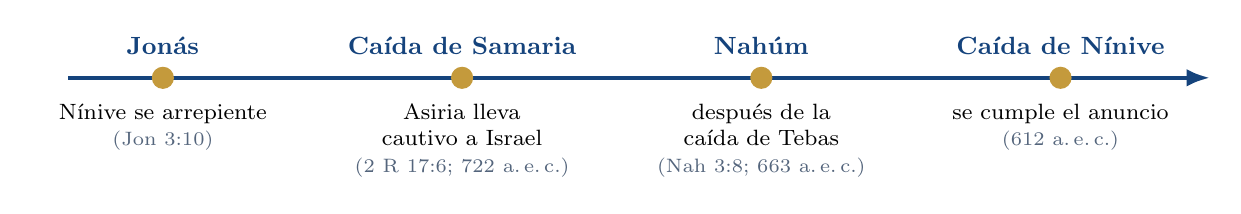
\begin{tikzpicture}[font=\small]
 \draw[line width=1.6pt,azul,-{Latex[length=3mm]}] (0,0) -- (14.5,0);
 \foreach \x/\t/\b/\r in {1.2/{Jonás}/{Nínive se arrepiente}/{Jon 3:10},
                          5.0/{Caída de Samaria}/{Asiria lleva cautivo a Israel}/{2 R 17:6; 722 a.\,e.\,c.},
                          8.8/{Nahúm}/{después de la caída de Tebas}/{Nah 3:8; 663 a.\,e.\,c.},
                          12.6/{Caída de Nínive}/{se cumple el anuncio}/{612 a.\,e.\,c.}}{
  \fill[dorado] (\x,0) circle (4pt);
  \node[above=5pt,font=\small\bfseries,text=azul] at (\x,0) {\t};
  \node[below=6pt,text width=3.2cm,align=center,font=\footnotesize] at (\x,0) {\b\\{\scriptsize\color{gris}(\r)}};}
\end{tikzpicture}\par
{\footnotesize\color{gris}\textit{Figura 1.} Nahúm en la historia de Asiria. \textit{Nota.} Elaboración propia con las fechas de Robertson (1990).}
\end{center}

\subsection{El Dios celoso y tardo para la ira}
\hebverso{אֵל קַנּוֹא וְנֹקֵם יְהוָה נֹקֵם יְהוָה וּבַעַל חֵמָה \\ יְהוָה אֶרֶךְ אַפַּיִם וּגְדָל־כֹּחַ וְנַקֵּה לֹא יְנַקֶּה}
\begin{verso}{Nahúm 1:2–3}
\SENOR{} es Dios celoso y vengador; \SENOR{} es vengador y lleno de indignación; se venga de sus adversarios, y guarda enojo para sus enemigos. \SENOR{} es tardo para la ira y grande en poder, y no tendrá por inocente al culpable. \SENOR{} marcha en la tempestad y el torbellino, y las nubes son el polvo de sus pies.
\end{verso}

\begin{filologia}{Nah 1:2--3}
\heb{קַנּוֹא} \emph{qanno} & \heb{קנא} & ``celoso'': el celo del esposo que no tolera rival (Éx 20:5; Jos 24:19). La ira nace del celo por lo que le pertenece. \\
\heb{נֹקֵם} \emph{noqem} & \heb{נקם} & ``vengador'', tres veces en el v.~2. No es revancha personal: es la reparación que el juez debe a la justicia (Dt 32:35). \\
\heb{בַּעַל חֵמָה} \emph{ba'al jemá} & \heb{יחם} & literalmente, ``señor de furor'' (RVR1960: ``lleno de indignación''). \emph{Jemá} es calor, ardor. \\
\heb{נוֹטֵר} \emph{noter} & \heb{נטר} & ``guarda'' el enojo: lo mantiene en reserva y no lo descarga de inmediato. \\
\heb{אֶרֶךְ אַפַּיִם} \emph{érej appáyim} & \heb{ארך}, \heb{אנף} & ``largo de narices'': lento para la ira. Es la fórmula de Éx 34:6. \\
\heb{וְנַקֵּה לֹא יְנַקֶּה} \emph{venaqqé lo yenaqqé} & \heb{נקה} & ``y absolver, no absolverá'': el infinitivo absoluto refuerza la negación. Cita Éx 34:7. \\
\end{filologia}

La paciencia de Dios (\emph{érej appáyim}) y su justicia (\emph{lo yenaqqé}) están en el mismo verso. La ira de Dios es lenta, pero no se anula. Nínive tuvo más de un siglo desde la predicación de Jonás; la paciencia no era indiferencia.

\subsection{¿Quién permanecerá?}
\hebverso{לִפְנֵי זַעְמוֹ מִי יַעֲמוֹד וּמִי יָקוּם בַּחֲרוֹן אַפּוֹ \\ חֲמָתוֹ נִתְּכָה כָאֵשׁ וְהַצֻּרִים נִתְּצוּ מִמֶּנּוּ}
\begin{verso}{Nahúm 1:6}
¿Quién permanecerá delante de su ira? ¿y quién quedará en pie en el ardor de su enojo? Su ira se derrama como fuego, y por él se hienden las peñas.
\end{verso}

\begin{filologia}{Nah 1:6}
\heb{זַעַם} \emph{za'am} & \heb{זעם} & ``indignación'': la ira que denuncia y condena. \\
\heb{חֲרוֹן אַף} \emph{jarón af} & \heb{חרה} & ``ardor de nariz'': la ira que se enciende. \\
\heb{נִתְּכָה} \emph{nittejá} & \heb{נתך} & ``se derrama''; el verbo se usa para el metal fundido (Ez 22:20--22). \\
\heb{מִי יַעֲמוֹד} \emph{mi ya'amod} & \heb{עמד} & ``¿quién permanecerá de pie?'': pregunta retórica cuya respuesta es ``nadie''. \\
\end{filologia}

La pregunta de Nahúm atraviesa la Escritura. Malaquías la repite ante la venida del Señor: ``¿Y quién podrá soportar el tiempo de su venida? ¿o quién podrá estar en pie cuando él se manifieste?'' (Mal 3:2). Apocalipsis la pone en boca de los reyes de la tierra: ``el gran día de su ira ha llegado; ¿y quién podrá sostenerse en pie?'' (Ap 6:17). Nahúm, sin embargo, no deja la pregunta sin salida:

\begin{verso}{Nahúm 1:7}
\SENOR{} es bueno, fortaleza en el día de la angustia; y conoce a los que en él confían.
\end{verso}

\precision{nah 1:2--8 forma un acróstico parcial: los versos siguen, con algunas irregularidades, el orden del alfabeto hebreo desde \heb{א} hasta \heb{כ} (Robertson, 1990). La forma sugiere un poema que dice ``todo'' sobre el Dios que juzga; la lectura de la forma como ``totalidad'' es una interpretación.}

\subsection{Bondad y severidad}
El mismo poema que muestra la ira muestra la bondad. Pablo, judío que lee a Israel cumplido en Cristo, pide mirar las dos caras a la vez:

\begin{verso}{Romanos 11:22}
Mira, pues, la bondad y la severidad de Dios; la severidad ciertamente para con los que cayeron, pero la bondad para contigo, si permaneces en esa bondad; pues de otra manera tú también serás cortado.
\end{verso}

\begin{filologia}{Ro 11:22}
\grc{ἀποτομία} \emph{apotomía} & \grc{τέμνω} & ``severidad'': de \grc{ἀποτέμνω}, ``cortar de raíz''. Un corte tajante (Bauer et~al., 2000). \\
\grc{χρηστότης} \emph{jrēstótēs} & \grc{χρηστός} & ``bondad'': benignidad que se hace útil al otro. \\
\end{filologia}

Separar la bondad de la severidad deforma a Dios. Un Dios solo severo sería un tirano; un Dios solo bondadoso sería indiferente al mal. Nahúm y Pablo ponen las dos en la misma frase.

%===================================================================
\section{La palabra: el vocabulario de la ira}

\subsection{Un campo con imágenes físicas}
El hebreo no tiene una sola palabra para la ira de Dios. Tiene un campo entero, y casi todas sus palabras son imágenes concretas: la nariz que resopla, el calor, el fuego, el agua que se desborda.

\begin{center}\small\renewcommand{\arraystretch}{1.25}
\begin{tabular}{@{}L{2.8cm}L{1.6cm}L{6.6cm}L{3.2cm}@{}}
\toprule
\textbf{Término} & \textbf{Raíz} & \textbf{Imagen y sentido} & \textbf{Ejemplo} \\ \midrule
\heb{אַף} \emph{af} & \heb{אנף} & nariz; la ira que se enciende & Nm 12:9; Sal 95:11 \\
\heb{חֵמָה} \emph{jemá} & \heb{יחם} & calor, veneno, furor & Nah 1:2, 6 \\
\heb{חָרוֹן} \emph{jarón} & \heb{חרה} & ardor, incendio & Éx 15:7; Nah 1:6 \\
\heb{עֶבְרָה} \emph{evrá} & \heb{עבר} & furia que pasa por encima, que se desborda & Sof 1:15 \\
\heb{קֶצֶף} \emph{qétsef} & \heb{קצף} & enojo, indignación & Nm 16:46 [17:11] \\
\heb{זַעַם} \emph{za'am} & \heb{זעם} & indignación que denuncia y condena & Nah 1:6 \\
\bottomrule
\end{tabular}\par\smallskip
{\footnotesize\color{gris}\textit{Tabla 1.} Vocabulario hebreo de la ira de Dios. \textit{Nota.} Sentidos según Koehler y Baumgartner (2001).}
\end{center}

\subsection{“Largo de narices”}
\hebverso{יְהוָה אֶרֶךְ אַפַּיִם וְרַב־חֶסֶד}
\begin{verso}{Números 14:18}
\SENOR, tardo para la ira y grande en misericordia, que perdona la iniquidad y la rebelión, aunque de ningún modo tendrá por inocente al culpable; que visita la maldad de los padres sobre los hijos hasta los terceros y hasta los cuartos.
\end{verso}

\begin{filologia}{Nm 14:18}
\heb{אַף} / \heb{אַפַּיִם} \emph{af} / \emph{appáyim} & \heb{אנף} & ``nariz'' / ``narices''. Cuando alguien se enoja, la nariz resopla y se ``enciende'': \heb{וַיִּחַר אַף} (\emph{vayyíjar af}), ``se encendió la ira'' (Nm 12:9). \\
\heb{אֶרֶךְ} \emph{érej} & \heb{ארך} & ``largo''. \emph{Érej appáyim}, ``largo de narices'', describe al que tarda en encenderse. \\
\heb{רַב־חֶסֶד} \emph{rav-jésed} & \heb{חסד} & ``grande en misericordia'': amor leal de pacto. \\
\end{filologia}

Moisés intercede por Israel después del informe de los espías citando a Dios mismo (Éx 34:6--7). No niega la justicia (``de ningún modo tendrá por inocente al culpable''); apela a la paciencia. Dios perdona, y aun así esa generación no entra en la tierra (Nm 14:20--23).

\subsection{Del hebreo a Pablo}
La Septuaginta traduce este campo sobre todo con dos palabras griegas, \grc{ὀργή} (\emph{orgē}) y \grc{θυμός} (\emph{thymós}). Pablo hereda el vocabulario y casi siempre usa \emph{orgē}; a menudo dice simplemente ``la ira'', sin más, para referirse al juicio final (Ro 5:9; 1~Ts 1:10).

\begin{center}
\begin{tikzpicture}[font=\small,node distance=0.8cm,
  b/.style={draw=azul,line width=0.8pt,fill=papiro,rounded corners=3pt,text width=3.6cm,align=center,inner sep=5pt}]
 \node[b] (h) {\textbf{Hebreo}\\ \heb{אַף} \emph{af}, \heb{חָרוֹן} \emph{jarón}, \heb{חֵמָה} \emph{jemá}};
 \node[b,right=of h] (l) {\textbf{Septuaginta}\\ \grc{ὀργή} \emph{orgē}\\ \grc{θυμός} \emph{thymós}};
 \node[b,right=of l] (p) {\textbf{Pablo}\\ \grc{ὀργή} (Ro 1:18; 5:9)\\ \grc{ὀργὴ καὶ θυμός} (Ro 2:8)};
 \draw[-{Latex[length=2.5mm]},dorado,line width=1.2pt] (h)--(l);
 \draw[-{Latex[length=2.5mm]},dorado,line width=1.2pt] (l)--(p);
\end{tikzpicture}\par
{\footnotesize\color{gris}\textit{Figura 2.} El vocabulario de la ira del hebreo a Pablo. \textit{Nota.} Elaboración propia.}
\end{center}

\precision{trench (1880) distinguió \emph{orgē}, la ira como disposición firme, de \emph{thymós}, el estallido de la pasión. La distinción ayuda, pero el uso no es rígido: Pablo pone las dos palabras juntas en Ro 2:8 (``ira y enojo''), y en sus listas de vicios \emph{thymós} describe la ira humana (Gá 5:20).}

%===================================================================
\section{El Nombre que revela la ira santa}

En la Escritura el nombre de Dios es la revelación de lo que él es (Éx 33:18--19). El mismo Nombre proclamado en el Sinaí contiene la paciencia y el juicio: ``tardo para la ira'' y ``de ningún modo tendrá por inocente al malvado'' (Éx 34:6--7). En el texto ancla, Nahúm repite tres veces el Nombre con el título ``vengador'' y llama a Dios \heb{בַּעַל חֵמָה} (\emph{ba'al jemá}), ``señor de furor'' (Nah 1:2). La Escritura forma con la ira otros títulos.

\subsection{“Dios de las venganzas”}
\hebverso{אֵל־נְקָמוֹת יְהוָה \\ אֵל נְקָמוֹת הוֹפִיעַ}
\begin{verso}{Salmo 94:1–2}
\SENOR{}, Dios de las venganzas, Dios de las venganzas, muéstrate. Engrandécete, oh Juez de la tierra; Da el pago a los soberbios.
\end{verso}

\begin{filologia}{Sal 94:1--2}
\heb{אֵל נְקָמוֹת} \emph{El neqamot} & \heb{נקם} & ``Dios de venganzas''; el plural intensifica. La \emph{neqamá} bíblica no es revancha personal: es la reparación que el juez debe al agraviado (Dt 32:35). \\
\heb{הוֹפִיעַ} \emph{hofí'a} & \heb{יפע} & ``resplandece'', ``muéstrate'': verbo de teofanía, el que describe a Dios cuando aparece para actuar (Dt 33:2; Sal 50:2; 80:1 [80:2]). \\
\heb{שֹׁפֵט הָאָרֶץ} \emph{shofet ha'árets} & \heb{שׁפט} & ``Juez de la tierra'': el título de Gn 18:25 (``el Juez de toda la tierra''). \\
\grc{ὁ θεὸς ἐκδικήσεων} & --- & la Septuaginta traduce ``el Dios de las vindicaciones'' (Sal 93:1 LXX), con la familia de \grc{ἐκδικ-} que usará Pablo. \\
\end{filologia}

El salmo explica por qué el salmista llama así a Dios: ``A la viuda y al extranjero matan, Y a los huérfanos quitan la vida'' (Sal 94:6). El nombre ``Dios de las venganzas'' no es una amenaza contra el débil, sino su esperanza. Si Dios no fuera el vengador de la viuda y del huérfano, la injusticia tendría la última palabra.

\subsection{“Dios de retribuciones”}
\hebverso{כִּי אֵל גְּמֻלוֹת יְהוָה שַׁלֵּם יְשַׁלֵּם}
\begin{verso}{Jeremías 51:56}
Porque vino destruidor contra ella, contra Babilonia, y sus valientes fueron apresados; el arco de ellos fue quebrado; porque \SENOR{}, Dios de retribuciones, dará la paga.
\end{verso}

\begin{filologiatexto}{Jer 51:56}
\heb{אֵל גְּמֻלוֹת} (\emph{El gemulot}) es ``Dios de retribuciones''; la raíz \heb{גמל} significa ``dar a cada uno lo que corresponde''. \heb{שַׁלֵּם יְשַׁלֵּם} (\emph{shallem yeshallem}) une el infinitivo absoluto y el verbo de la raíz \heb{שׁלם}: ``ciertamente pagará''. Es la misma raíz de \emph{shalom}: la retribución restablece lo que la injusticia quebró.
\end{filologiatexto}

El oráculo es contra Babilonia, el imperio que destruyó Jerusalén. La ira de Dios contra el opresor es también fidelidad a su pueblo.

\subsection{“Cuyo nombre es Celoso”}
\hebverso{כִּי יְהוָה קַנָּא שְׁמוֹ אֵל קַנָּא הוּא}
\begin{verso}{Éxodo 34:14}
Porque no te has de inclinar a ningún otro dios, pues \SENOR{}, cuyo nombre es Celoso, Dios celoso es.
\end{verso}

\begin{filologiatexto}{Éx 34:14}
\heb{קַנָּא שְׁמוֹ} (\emph{qanná shemó}): ``Celoso (es) su nombre''. Como con ``Santo'' (Is 57:15), el atributo se vuelve Nombre. El verso está en el mismo capítulo de las trece medidas (Éx 34:6--7). La ira nace del celo; el celo tendrá su propio capítulo.
\end{filologiatexto}

\precision{la tradición rabínica asoció cada nombre de Dios con una de sus obras. En \emph{Shemot Rabá} 3:6, Rabí Abbá bar Memel pone en boca de Dios: ``Cuando juzgo a las criaturas, soy llamado \emph{Elohim}; cuando hago guerra contra los impíos, soy llamado \emph{Tsevaot}; cuando suspendo el castigo por los pecados del hombre, soy llamado \emph{El Shadday}; y cuando tengo misericordia de mi mundo, soy llamado \SENOR{}''. Es una lectura rabínica, no una etimología: une el juicio, la guerra contra el mal, la paciencia y la misericordia en el mismo Dios.}

\subsection{El Señor vengador y el nombre de Jesús, con Pablo}
Pablo hereda el vocabulario del Dios de las venganzas. Cita Dt 32:35 (``Mía es la venganza, yo pagaré, dice el Señor'', Ro 12:19) y advierte a los tesalonicenses:

\begin{verso}{1 Tesalonicenses 4:6}
que ninguno agravie ni engañe en nada a su hermano; porque el Señor es vengador de todo esto, como ya os hemos dicho y testificado.
\end{verso}

\begin{filologiatexto}{1~Ts 4:6}
\grc{ἔκδικος κύριος} (\emph{ékdikos kýrios}): ``vengador (es el) Señor''. \grc{ἔκδικος} pertenece a la misma familia que \grc{ἐκδικήσεων} de Sal 93:1 LXX y \grc{ἐκδίκησις} de Ro 12:19. Pablo aplica a ``el Señor'' el título del Sal 94.
\end{filologiatexto}

Pero el mismo Pablo anuncia otro Nombre frente a esa ira: ``a Jesús, quien nos libra de la ira venidera'' (\grc{Ἰησοῦν τὸν ῥυόμενον ἡμᾶς ἐκ τῆς ὀργῆς τῆς ἐρχομένης}, 1~Ts 1:10). El nombre de Jesús, en hebreo \heb{יְהוֹשׁוּעַ} (\emph{Yehoshúa}) o \heb{יֵשׁוּעַ} (\emph{Yeshúa}), une el Nombre divino con la raíz \heb{ישׁע}, ``salvar'': ``el \SENOR{} salva''. Así lo explica el ángel: ``llamarás su nombre JESÚS, porque él salvará a su pueblo de sus pecados'' (Mt 1:21). El Dios de las venganzas da a su Hijo un nombre de salvación.

\precision{en 1~Ts 4:6, ``el Señor'' puede referirse a Dios o a Cristo; los comentaristas se dividen. La explicación del nombre de Jesús por la raíz \heb{ישׁע} es la que da el propio Mateo; la relación con el título de Sal 94:1 es lectura propia.}

\begin{center}
\small\renewcommand{\arraystretch}{1.2}
\begin{tabular}{@{}L{4.2cm}L{3.6cm}L{3.0cm}L{4.6cm}@{}}
\toprule
\textbf{Nombre o título} & \textbf{Hebreo / griego} & \textbf{Texto} & \textbf{Qué revela} \\ \midrule
``Tardo para la ira \ldots{} no tendrá por inocente'' & \heb{אֶרֶךְ אַפַּיִם}; \heb{וְנַקֵּה לֹא יְנַקֶּה} & Éx 34:6--7 & Paciencia y juicio en el Nombre \\
``Dios celoso y vengador'', ``señor de furor'' & \heb{אֵל קַנּוֹא וְנֹקֵם}; \heb{בַּעַל חֵמָה} & Nah 1:2 & El texto ancla \\
``Cuyo nombre es Celoso'' & \heb{קַנָּא שְׁמוֹ} & Éx 34:14 & La ira nace del celo \\
``Dios de las venganzas'' & \heb{אֵל נְקָמוֹת} & Sal 94:1 & Esperanza del oprimido \\
``Juez de la tierra'' & \heb{שֹׁפֵט הָאָרֶץ} & Sal 94:2; Gn 18:25 & Juicio justo \\
``Dios de retribuciones'' & \heb{אֵל גְּמֻלוֹת} & Jer 51:56 & Da a cada uno lo suyo \\
``El Señor es vengador'' & \grc{ἔκδικος κύριος} & 1~Ts 4:6; Ro 12:19 & Pablo hereda el título \\
``Jesús, que nos libra de la ira'' & \grc{Ἰησοῦς}, \heb{יֵשׁוּעַ} & 1~Ts 1:10; Mt 1:21 & El Nombre que salva \\ \bottomrule
\end{tabular}\par\smallskip
{\footnotesize\color{gris}\textit{Tabla.} La ira santa en los nombres de Dios. \textit{Nota.} Elaboración propia.}
\end{center}

%===================================================================
\section{Definición}

\subsection{Lo que la ira de Dios no es}
La palabra ``ira'' trae a la mente la experiencia humana: el grito, el portazo, el rencor. La ira de Dios no es eso.
\begin{itemize}
\item No es pérdida de control ni explosión emocional (D.~A. Carson).
\item No es caprichosa, impulsiva ni irracional.
\item No es venganza humana ni temperamento explosivo.
\item Es una reacción decidida, voluntaria y justa contra todo lo que deshonra a Dios y destruye su creación.
\end{itemize}

\begin{verso}{Santiago 1:19–20}
Por esto, mis amados hermanos, todo hombre sea pronto para oír, tardo para hablar, tardo para airarse; porque la ira del hombre no obra la justicia de Dios.
\end{verso}

\begin{filologiatexto}{Stg 1:20}
\grc{ὀργὴ γὰρ ἀνδρὸς δικαιοσύνην θεοῦ οὐκ ἐργάζεται}. La ira del varón (\grc{ὀργὴ ἀνδρός}) no produce la justicia de Dios. Santiago usa la misma palabra, \emph{orgē}, para la ira humana y para la divina; la diferencia no está en el término, sino en su fuente y en su fin. La ira humana sirve al yo; la de Dios es su justicia en acción.
\end{filologiatexto}

\subsection{Lo que la ira de Dios es}
\begin{tcolorbox}[colback=papiro,colframe=azul,boxrule=1pt,arc=3pt,fonttitle=\bfseries\small,title=Definición]
La ira de Dios es la respuesta santa, justa y deliberada de Dios ante el pecado. Surge de su santidad y de su justicia ofendidas, es continua y a la vez futura, y no niega su amor ni su misericordia: es coherente con su santidad.
\end{tcolorbox}

\begin{center}\small\renewcommand{\arraystretch}{1.25}
\begin{tabular}{@{}L{2.6cm}L{7.4cm}L{4.4cm}@{}}
\toprule
\textbf{Rasgo} & \textbf{Qué afirma} & \textbf{Textos} \\ \midrule
Santa & nace de su santidad, no de un temperamento & Is 6:3; Hab 1:13 \\
Justa & da a cada uno lo que corresponde & Gn 18:25; Ro 2:5--6 \\
Presente & ``se revela'', en presente & Ro 1:18 \\
Futura & ``el día de la ira'' & Ro 2:5; Ap 6:17 \\
Lenta & tarda en encenderse & Nah 1:3; Nm 14:18 \\
\bottomrule
\end{tabular}\end{center}

\subsection{¿Perfección eterna o reacción?}
El material de estudio de esta serie llama a la ira un \emph{atributo secundario}: no es parte esencial del ser de Dios como el amor o la santidad, sino una respuesta santa y justa al pecado. Pink, en cambio, la llama una perfección divina, tan real como su fidelidad, su poder o su misericordia (Pink, 2020). Las dos afirmaciones se concilian si se distingue la raíz de la manifestación. Lo eterno es la santidad y la justicia de Dios; la ira es esa misma perfección cuando encuentra el pecado. Antes de que hubiera pecado no había contra qué airarse, pero Dios ya era el que se airaría contra él.

\precision{la conciliación es una propuesta propia de este capítulo. La serie entiende todos los atributos como perfecciones eternas; aquí la ira se entiende como perfección eterna en su raíz y como reacción en su manifestación.}

\subsection{La ira entre los atributos}
La ira no compite con los demás atributos. La santidad la origina, la justicia la mide, y el amor y la misericordia la demoran y le abren una salida.

\begin{center}\small\renewcommand{\arraystretch}{1.25}
\begin{tabular}{@{}L{2.8cm}L{8.2cm}L{3.4cm}@{}}
\toprule
\textbf{Atributo} & \textbf{Relación con la ira} & \textbf{Texto} \\ \midrule
Santidad & separación absoluta del pecado y perfección moral; todo lo que Dios hace es coherente con ella & Is 6:3 \\
Justicia & exige que el pecado sea castigado; no puede dejarlo impune & Dt 32:4 \\
Amor & su inclinación a buscar el bien del hombre aun cuando no lo merece & 1~Jn 4:8 \\
Misericordia & Dios detiene el castigo merecido y da tiempo para el arrepentimiento & Sal 103:8 \\
\bottomrule
\end{tabular}\end{center}

\begin{verso}{Deuteronomio 32:4}
Él es la Roca, cuya obra es perfecta, Porque todos sus caminos son rectitud; Dios de verdad, y sin ninguna iniquidad en él; Es justo y recto.
\end{verso}

\begin{verso}{Salmo 103:8}
Misericordioso y clemente es \SENOR; Lento para la ira, y grande en misericordia.
\end{verso}

\subsection{Clasificación}
En la clasificación de esta obra, la ira pertenece a los atributos de la \destacar{relación con el ser humano}: responde a la pregunta ``¿cómo se revela?''. Es \destacar{incomunicable} como juicio: ``Mía es la venganza, yo pagaré'' (Ro 12:19). El creyente participa de ella solo como un reflejo limitado y vigilado: ``Airaos, pero no pequéis'' (Ef 4:26).

%===================================================================
\section{Teología: la exposición de Pink}

Pink dedica un capítulo de \emph{Los atributos de Dios} a la ira. Su recorrido puede resumirse en cinco pasos (Pink, 2020):
\begin{enumerate}
\item La ira es una perfección del carácter divino, tan real como su fidelidad, su poder o su misericordia. Un Dios que no se airara contra el pecado no sería santo.
\item La Escritura habla de ella con más frecuencia que de su amor y su ternura; callarla es mutilar la revelación.
\item Es el aborrecimiento eterno de Dios hacia toda injusticia, y por eso es santa y justa.
\item Se ha manifestado en la ley, en la historia y, sobre todo, en la cruz.
\item Meditarla tiene tres frutos: ver la gravedad del pecado, temer a Dios con reverencia y agradecer la liberación.
\end{enumerate}

\begin{verso}{Salmo 90:11}
¿Quién conoce el poder de tu ira, Y tu indignación según que debes ser temido?
\end{verso}

\begin{verso}{1 Tesalonicenses 1:10}
y esperar de los cielos a su Hijo, al cual resucitó de los muertos, a Jesús, quien nos libra de la ira venidera.
\end{verso}

\precision{el resumen del recorrido de Pink está en palabras propias; no es una cita textual.}

%===================================================================
\section{Un encuentro en la historia de Israel}

La ira de Dios en Israel no es una idea abstracta: tiene lugares, nombres y fechas. Y en casi todos los episodios aparece también un intercesor o un camino de escape.

\begin{center}
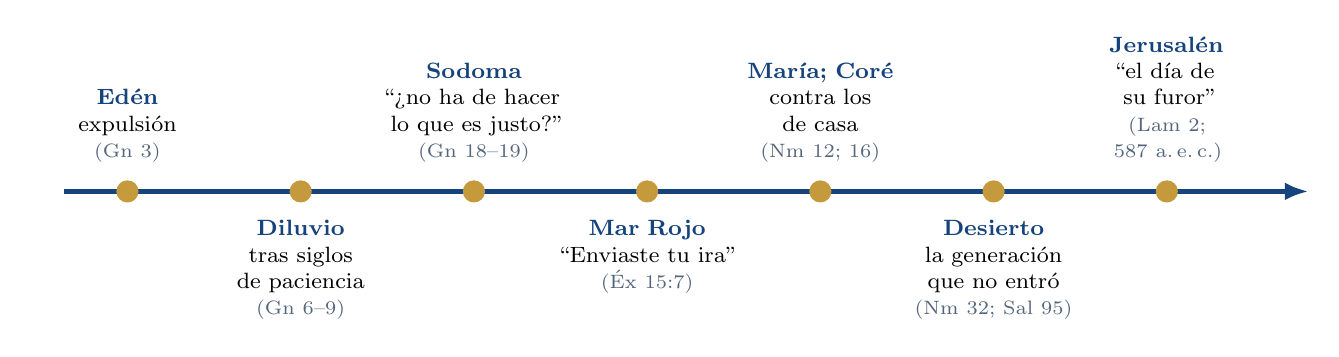
\begin{tikzpicture}[font=\footnotesize]
 \draw[line width=1.6pt,azul,-{Latex[length=3mm]}] (-0.4,0) -- (15.4,0);
 \foreach \x/\t/\b/\r/\pos in {0.4/{Edén}/{expulsión}/{Gn 3}/above,
   2.6/{Diluvio}/{tras siglos de paciencia}/{Gn 6--9}/below,
   4.8/{Sodoma}/{``¿no ha de hacer lo que es justo?''}/{Gn 18--19}/above,
   7.0/{Mar Rojo}/{``Enviaste tu ira''}/{Éx 15:7}/below,
   9.2/{María; Coré}/{contra los de casa}/{Nm 12; 16}/above,
   11.4/{Desierto}/{la generación que no entró}/{Nm 32; Sal 95}/below,
   13.6/{Jerusalén}/{``el día de su furor''}/{Lam 2; 587 a.\,e.\,c.}/above}{
  \fill[dorado] (\x,0) circle (4pt);
  \node[\pos=7pt,text width=2.3cm,align=center] at (\x,0) {\textbf{\textcolor{azul}{\t}}\\ \b\\ {\scriptsize\color{gris}(\r)}};}
\end{tikzpicture}\par
{\footnotesize\color{gris}\textit{Figura 3.} Hechos históricos de la ira de Dios. \textit{Nota.} Elaboración propia.}
\end{center}

\subsection{En el Mar Rojo}
\hebverso{תְּשַׁלַּח חֲרֹנְךָ יֹאכְלֵמוֹ כַּקַּשׁ}
\begin{verso}{Éxodo 15:6–7}
Tu diestra, oh \SENOR, ha sido magnificada en poder; Tu diestra, oh \SENOR, ha quebrantado al enemigo. Y con la grandeza de tu poder has derribado a los que se levantaron contra ti. Enviaste tu ira; los consumió como a hojarasca.
\end{verso}

\begin{filologia}{Éx 15:7}
\heb{חֲרֹנְךָ} \emph{jaronja} & \heb{חרה} & ``tu ardor'' (RVR1960: ``tu ira''): la ira como fuego. \\
\heb{תְּשַׁלַּח} \emph{teshallaj} & \heb{שׁלח} & ``envías'': la ira es un enviado de Dios, no un descontrol. \\
\heb{קַשׁ} \emph{qash} & \heb{קשׁשׁ} & ``hojarasca, paja'': lo que el fuego consume sin resistencia. \\
\end{filologia}

Es el primer canto de Israel, y la ira de Dios aparece en él como salvación. La ira que destruye al opresor libra al oprimido.

\subsection{Contra los de casa: María y Coré}
La ira de Dios no se dirige solo contra los enemigos de Israel. Cuando María y Aarón murmuran contra Moisés, ``la ira de \SENOR{} se encendió contra ellos; y se fue'' (Nm 12:9; \heb{וַיִּחַר אַף יְהוָה בָּם}, ``se encendió la nariz del \SENOR{} contra ellos''). Cuando Coré, Datán y Abiram se rebelan, la tierra los traga:

\begin{verso}{Números 16:32–33}
Abrió la tierra su boca, y los tragó a ellos, a sus casas, a todos los hombres de Coré, y a todos sus bienes. Y ellos, con todo lo que tenían, descendieron vivos al Seol, y los cubrió la tierra, y perecieron de en medio de la congregación.
\end{verso}

Pedro aplica este principio al pueblo de Dios del nuevo pacto:

\begin{verso}{1 Pedro 4:17}
Porque es tiempo de que el juicio comience por la casa de Dios; y si primero comienza por nosotros, ¿cuál será el fin de aquellos que no obedecen al evangelio de Dios?
\end{verso}

\begin{filologiatexto}{1~P 4:17}
\grc{κρίμα} (\emph{krima}; Strong G2917), ``juicio'': la sentencia y su ejecución, resultado de \grc{κρίνω}, ``juzgar'' (Strong, 1890; Bauer et~al., 2000). El juicio comienza por la casa de Dios porque la cercanía no exime: aumenta la responsabilidad.
\end{filologiatexto}

\subsection{Entre los muertos y los vivos}
``El día siguiente'' de la rebelión de Coré, toda la congregación murmura contra Moisés y Aarón: ``Vosotros habéis dado muerte al pueblo de \SENOR'' (Nm 16:41). Dios responde: ``Apartaos de en medio de esta congregación, y los consumiré en un momento'' (Nm 16:45). Entonces ocurre una de las escenas más intensas de la Torá:

\hebverso{כִּי־יָצָא הַקֶּצֶף מִלִּפְנֵי יְהוָה הֵחֵל הַנָּגֶף \\ וַיַּעֲמֹד בֵּין־הַמֵּתִים וּבֵין הַחַיִּים וַתֵּעָצַר הַמַּגֵּפָה}
\begin{verso}{Números 16:46–48 [17:11–13]}
Y dijo Moisés a Aarón: Toma el incensario, y pon en él fuego del altar, y sobre él pon incienso, y ve pronto a la congregación, y haz expiación por ellos, porque el furor ha salido de la presencia de \SENOR; la mortandad ha comenzado. Entonces tomó Aarón el incensario, como dijo Moisés, y corrió en medio de la congregación; y he aquí que la mortandad había comenzado en el pueblo; y él puso incienso, e hizo expiación por el pueblo, y se puso entre los muertos y los vivos; y cesó la mortandad.
\end{verso}

\begin{filologia}{Nm 16:46--48}
\heb{הַקֶּצֶף} \emph{haqqétsef} & \heb{קצף} & ``el furor'' que ``salió'' de la presencia del \SENOR: la ira casi personificada. \\
\heb{הַנָּגֶף} \emph{hannégef} & \heb{נגף} & ``el golpe, la plaga'' (RVR1960: ``la mortandad''). \\
\heb{וְכַפֵּר} \emph{vejapper} & \heb{כפר} & ``y haz expiación'': la misma raíz de \emph{Yom Kippur}. \\
\heb{וַיַּעֲמֹד בֵּין} \emph{vayya'amod beyn} & \heb{עמד} & ``y se puso de pie entre'': el sacerdote ocupa el espacio entre la ira y el pueblo. \\
\heb{וַתֵּעָצַר} \emph{vatte'atsar} & \heb{עצר} & ``y fue detenida'' la plaga. \\
\end{filologia}

La ira de Dios avanza y alguien se pone en medio. Murieron catorce mil setecientos (Nm 16:49), pero la plaga se detuvo donde estaba el sacerdote con el fuego del altar. La misma escena que muestra la ira muestra que Dios provee el camino para detenerla.

\begin{center}
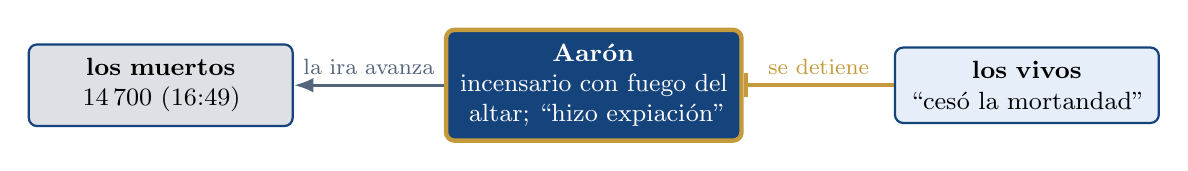
\begin{tikzpicture}[font=\small,
  b/.style={draw=azul,line width=0.8pt,fill=papiro,rounded corners=3pt,text width=3.0cm,align=center,inner sep=5pt}]
 \node[b,fill=gris!20] (m) at (0,0) {\textbf{los muertos}\\ 14\,700 (16:49)};
 \node[draw=dorado,line width=1.6pt,fill=azul,text=white,rounded corners=3pt,text width=3.4cm,align=center,inner sep=5pt] (a) at (5.5,0) {\textbf{Aarón}\\ incensario con fuego del altar; ``hizo expiación''};
 \node[b,fill=celeste!15] (v) at (11,0) {\textbf{los vivos}\\ ``cesó la mortandad''};
 \draw[-{Latex[length=2.5mm]},gris,line width=1.2pt] (a)--node[above,font=\footnotesize]{la ira avanza}(m);
 \draw[{Bar[width=3mm]}-,dorado,line width=1.4pt] (a)--node[above,font=\footnotesize]{se detiene}(v);
\end{tikzpicture}\par
{\footnotesize\color{gris}\textit{Figura 4.} Nm 16:46--48 [17:11--13]. \textit{Nota.} Elaboración propia.}
\end{center}

\precision{ver en Aarón una figura de Cristo, que se pone entre la ira y el pueblo, es una lectura tipológica propia; el texto de Números no la hace.}

\subsection{La generación que no entró}
La ira de Dios tuvo también una forma lenta: cuarenta años de desierto. Moisés la recuerda a los hijos de esa generación cuando las tribus de Rubén y Gad quieren quedarse al otro lado del Jordán:

\begin{verso}{Números 32:13–15}
Y la ira de \SENOR{} se encendió contra Israel, y los hizo andar errantes cuarenta años por el desierto, hasta que fue acabada toda aquella generación que había hecho mal delante de \SENOR. Y he aquí, vosotros habéis sucedido en lugar de vuestros padres, prole de hombres pecadores, para añadir aún a la ira de \SENOR{} contra Israel. Si os volviereis de en pos de él, él volverá otra vez a dejaros en el desierto, y destruiréis a todo este pueblo.
\end{verso}

El mismo hecho aparece en Deuteronomio y en los Salmos:

\begin{verso}{Deuteronomio 1:34–35}
Y oyó \SENOR{} la voz de vuestras palabras, y se enojó, y juró diciendo: No verá hombre alguno de estos, de esta mala generación, la buena tierra que juré que había de dar a vuestros padres.
\end{verso}

\hebverso{אֲשֶׁר־נִשְׁבַּעְתִּי בְאַפִּי אִם־יְבֹאוּן אֶל־מְנוּחָתִי}
\begin{verso}{Salmo 95:10–11}
Cuarenta años estuve disgustado con la nación, Y dije: Pueblo es que divaga de corazón, Y no conocen mis caminos. Por tanto, juré en mi furor Que no entrarían en mi reposo.
\end{verso}

\begin{filologia}{Dt 1:34; Sal 95:11}
\heb{וַיִּקְצֹף} \emph{vayyiqtsof} & \heb{קצף} & ``y se indignó'' (Dt 1:34). \\
\heb{וַיִּשָּׁבַע} \emph{vayyishava} & \heb{שׁבע} & ``y juró'': la ira se expresa como juramento, una decisión firme y no un arrebato. \\
\heb{בְאַפִּי} \emph{ve'appi} & \heb{אנף} & ``en mi furor'', literalmente ``en mi nariz'' (Sal 95:11). \\
\heb{מְנוּחָתִי} \emph{menujatí} & \heb{נוח} & ``mi reposo'': la tierra prometida como descanso de Dios. \\
\end{filologia}

Moisés habla a los hijos de esa generación: la ira de Dios en la historia es también una advertencia para los que vienen después. Hebreos lee el Sal 95 del mismo modo (He 3:7--4:11).

\subsection{Sodoma: el Juez de toda la tierra}
\begin{verso}{Génesis 18:20}
Entonces \SENOR{} le dijo: Por cuanto el clamor contra Sodoma y Gomorra se aumenta más y más, y el pecado de ellos se ha agravado en extremo.
\end{verso}

Dios no juzga sin examinar: ``descenderé ahora, y veré'' (Gn 18:21). Abraham intercede seis veces, de cincuenta justos a diez, y en el centro de su oración pone una pregunta:

\hebverso{הֲשֹׁפֵט כָּל־הָאָרֶץ לֹא יַעֲשֶׂה מִשְׁפָּט}
\begin{verso}{Génesis 18:25}
Lejos de ti el hacer tal, que hagas morir al justo con el impío, y que sea el justo tratado como el impío; nunca tal hagas. El Juez de toda la tierra, ¿no ha de hacer lo que es justo?
\end{verso}

\begin{filologia}{Gn 18:25}
\heb{חָלִלָה לְּךָ} \emph{jalila leja} & \heb{חלל} & ``lejos de ti'': fórmula de rechazo enfático; ``sería profano para ti''. \\
\heb{צַדִּיק עִם־רָשָׁע} \emph{tsaddiq im-rasha} & \heb{צדק}, \heb{רשׁע} & ``el justo con el impío'': el par que Abraham no puede aceptar que se confunda. \\
\heb{שֹׁפֵט} / \heb{מִשְׁפָּט} \emph{shofet} / \emph{mishpat} & \heb{שׁפט} & ``juez'' / ``juicio''. El Juez hará juicio: la ira de Dios es un acto judicial. \\
\end{filologia}

\begin{verso}{Génesis 18:32}
Y volvió a decir: No se enoje ahora mi Señor, si hablare solamente una vez: quizá se hallarán allí diez. No la destruiré, respondió, por amor a los diez.
\end{verso}

\subsection{Lamentaciones: el día de su furor}
La ira de Dios alcanzó también a Jerusalén, el templo y el trono de David. Lamentaciones llora la destrucción del 587~a.\,e.\,c.:

\hebverso{אֵיכָה יָעִיב בְּאַפּוֹ אֲדֹנָי אֶת־בַּת־צִיּוֹן}
\begin{verso}{Lamentaciones 2:1}
¡Cómo oscureció el Señor en su furor a la hija de Sion! Derribó del cielo a la tierra la hermosura de Israel, Y no se acordó del estrado de sus pies en el día de su furor.
\end{verso}

\begin{verso}{Lamentaciones 2:6}
Quitó su tienda como enramada de huerto; Destruyó el lugar en donde se congregaban; \SENOR{} ha hecho olvidar las fiestas solemnes y los días de reposo en Sion, Y en el ardor de su ira ha desechado al rey y al sacerdote.
\end{verso}

\begin{filologiatexto}{Lam 2:1}
\heb{אֵיכָה} (\emph{ejá}), ``¡cómo!'', es el grito del lamento y da nombre al libro en hebreo. \heb{יָעִיב בְּאַפּוֹ} (\emph{ya'iv be'appó}): ``nubló en su ira''. Lamentaciones 2 es un acróstico: cada verso comienza con una letra del alfabeto, de \heb{א} a \heb{ת}. El dolor se ordena letra por letra (Berlin, 2002).
\end{filologiatexto}

La ira llega al templo, a las fiestas, al rey y al sacerdote. Nada santo protege a quien vive sin el Santo.

%===================================================================
\section{Yom Kipur: una respuesta temporal}

\subsection{El Día de la Expiación}
Frente a la ira, Dios dio a Israel un día para la expiación. En Levítico 16, el sumo sacerdote entra una vez al año al Lugar Santísimo con sangre para cubrir el pecado del pueblo.

\hebverso{אַךְ בֶּעָשׂוֹר לַחֹדֶשׁ הַשְּׁבִיעִי הַזֶּה יוֹם הַכִּפֻּרִים הוּא}
\begin{verso}{Levítico 23:27–29}
A los diez días de este mes séptimo será el día de expiación; tendréis santa convocación, y afligiréis vuestras almas, y ofreceréis ofrenda encendida a \SENOR. Ningún trabajo haréis en este día; porque es día de expiación, para reconciliaros delante de \SENOR{} vuestro Dios. Porque toda persona que no se afligiere en este mismo día, será cortada de su pueblo.
\end{verso}

\begin{filologia}{Lv 23:27--29}
\heb{כָּפַר} / \heb{כִּפֶּר} \emph{kafar} / \emph{kipper} & \heb{כפר} & ``cubrir, limpiar, purgar la culpa''. En \emph{Yom Kippur} el sumo sacerdote rociaba sangre para cubrir el pecado del pueblo y permitir la comunión con Dios. \\
\heb{יוֹם הַכִּפֻּרִים} \emph{Yom hakkippurim} & \heb{כפר} & ``día de las expiaciones'': el plural intensifica. \\
\heb{כַּפֹּרֶת} \emph{kapporet} & \heb{כפר} & la tapa del arca, el propiciatorio, donde se rociaba la sangre (Lv 16:14--15). \\
\heb{תְּעַנּוּ} / \heb{תְעֻנֶּה} \emph{te'annú} / \emph{te'unné} & \heb{ענה} & ``afligiréis'' / ``se afligiere'': ayunar, humillarse, reconocer el pecado. \\
\heb{וְנִכְרְתָה} \emph{venijretá} & \heb{כרת} & ``será cortada'': excluida de la comunidad del pacto y expuesta al juicio divino. \\
\end{filologia}

\subsection{Sentido teológico}
Afligirse era la actitud que Dios exigía para recibir el beneficio de la expiación. Quien no se afligía mostraba desprecio por el sacrificio y por la santidad de Dios. ``Será cortada de su pueblo'' significa quedar excluido de la comunidad del pacto y expuesto al juicio divino; podía implicar la muerte física o la separación total bajo el desagrado de Dios. Es una manifestación directa de la ira: el que rechaza el camino que Dios proveyó para aplacarla queda bajo condenación.

En Yom Kipur se juntan tres atributos:
\begin{itemize}
\item \textbf{Santidad:} el pecado no puede entrar al Lugar Santísimo.
\item \textbf{Justicia:} la sangre es derramada por la culpa.
\item \textbf{Amor y misericordia:} Dios provee un sustituto.
\end{itemize}

\begin{verso}{Levítico 16:30}
Porque en este día se hará expiación por vosotros, y seréis limpios de todos vuestros pecados delante de \SENOR.
\end{verso}

\subsection{Una expiación insuficiente}
Pero esa expiación era insuficiente y temporal: debía repetirse cada año, porque la sangre de animales no podía quitar el pecado de manera definitiva.

\begin{verso}{Hebreos 10:1}
Porque la ley, teniendo la sombra de los bienes venideros, no la imagen misma de las cosas, nunca puede, por los mismos sacrificios que se ofrecen continuamente cada año, hacer perfectos a los que se acercan.
\end{verso}

\begin{verso}{Hebreos 10:4}
porque la sangre de los toros y de los machos cabríos no puede quitar los pecados.
\end{verso}

%===================================================================
\section{La ira de Dios en Cristo, leída con Pablo}

\subsection{La ira se revela}
Pablo, judío formado en las Escrituras de Israel, abre la exposición de su evangelio con la ira de Dios. Antes de hablar de la gracia, muestra por qué se necesita.

\begin{verso}{Romanos 1:18}
Porque la ira de Dios se revela desde el cielo contra toda impiedad e injusticia de los hombres que detienen con injusticia la verdad.
\end{verso}

\begin{filologia}{Ro 1:17--18}
\grc{ἀποκαλύπτεται} \emph{apokalýptetai} & \grc{καλύπτω} & ``se revela'', en presente. El mismo verbo del v.~17: ``en el evangelio la justicia de Dios se revela''. Justicia e ira se revelan una al lado de la otra. \\
\grc{ὀργὴ θεοῦ} \emph{orgē theoû} & --- & ``ira de Dios'': no un sentimiento pasajero, sino su oposición judicial al pecado (Moo, 1996). \\
\grc{ἀσέβεια} \emph{asébeia} & \grc{σέβομαι} & ``impiedad'': falta de reverencia hacia Dios. \\
\grc{κατεχόντων} \emph{katejóntōn} & \grc{κατέχω} & ``los que detienen'': retienen o suprimen la verdad que conocen. \\
\end{filologia}

La ira es continua (``se revela'', en presente) y a la vez futura (``el día de la ira'', Ro 2:5). No niega el amor ni la misericordia de Dios; es coherente con su santidad.

\subsection{“Los entregó”}
La humanidad no agradeció ni recibió:

\begin{verso}{Romanos 1:21}
Pues habiendo conocido a Dios, no le glorificaron como a Dios, ni le dieron gracias, sino que se envanecieron en sus razonamientos, y su necio corazón fue entenebrecido.
\end{verso}

La respuesta de Dios es sorprendente. Pablo no describe primero fuego del cielo, sino una entrega: \grc{παρέδωκεν αὐτοὺς ὁ θεός}, ``Dios los entregó'', tres veces (Ro 1:24, 26, 28). La ira presente consiste en dejar al hombre en manos de lo que eligió. Muchos siguen suprimiendo la verdad y viviendo en desobediencia; por eso, aunque la cruz proveyó una salvación suficiente, no todos están cubiertos por esa sangre.

\subsection{La justicia y la paz se besaron}
\hebverso{חֶסֶד־וֶאֱמֶת נִפְגָּשׁוּ צֶדֶק וְשָׁלוֹם נָשָׁקוּ}
\begin{verso}{Salmo 85:10 [85:11]}
La misericordia y la verdad se encontraron; La justicia y la paz se besaron.
\end{verso}

\begin{filologia}{Sal 85:10}
\heb{נִפְגָּשׁוּ} \emph{nifgashu} & \heb{פגשׁ} & ``se encontraron'': dos que venían por caminos distintos. \\
\heb{נָשָׁקוּ} \emph{nashaqu} & \heb{נשׁק} & ``se besaron'': reconciliación plena. \\
\heb{צֶדֶק} \emph{tsédeq} & \heb{צדק} & ``justicia'': contiene la ira de Dios contra el pecado. \\
\heb{שָׁלוֹם} \emph{shalom} & \heb{שׁלם} & ``paz'': nace de la misericordia (\emph{jésed}). \\
\end{filologia}

La justicia de Dios contiene su ira, y la paz nace de su misericordia. Dios es justo, y por eso debe castigar; Dios es amor, y por eso quiere perdonar. Estos dos puntos se cumplen en el madero: se castiga el pecado y se perdona al pecador.

\begin{center}
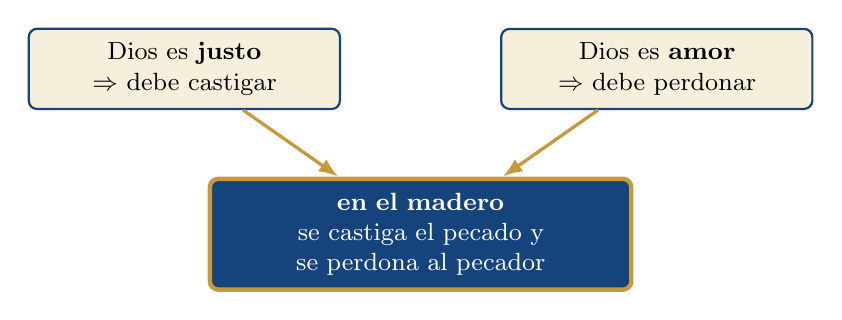
\begin{tikzpicture}[font=\small,
  b/.style={draw=azul,line width=0.8pt,fill=papiro,rounded corners=3pt,text width=3.6cm,align=center,inner sep=5pt}]
 \node[b] (j) at (-3,1.6) {Dios es \textbf{justo}\\ $\Rightarrow$ debe castigar};
 \node[b] (a) at (3,1.6) {Dios es \textbf{amor}\\ $\Rightarrow$ debe perdonar};
 \node[draw=dorado,line width=1.6pt,fill=azul,text=white,rounded corners=3pt,text width=5cm,align=center,inner sep=5pt] (m) at (0,-0.5) {\textbf{en el madero}\\ se castiga el pecado y se perdona al pecador};
 \draw[-{Latex[length=2.5mm]},dorado,line width=1.2pt] (j)--(m);
 \draw[-{Latex[length=2.5mm]},dorado,line width=1.2pt] (a)--(m);
\end{tikzpicture}\par
{\footnotesize\color{gris}\textit{Figura 5.} Justicia y amor en la cruz. \textit{Nota.} Elaboración propia a partir del comentario del autor de la serie al Sal 85:10.}
\end{center}

\precision{el Salmo 85 pide la restauración de Israel después del castigo (Sal 85:1--7); su aplicación a la cruz es una lectura cristológica propia.}

\subsection{La propiciación}
\begin{verso}{Romanos 3:23–26}
por cuanto todos pecaron, y están destituidos de la gloria de Dios, siendo justificados gratuitamente por su gracia, mediante la redención que es en Cristo Jesús, a quien Dios puso como propiciación por medio de la fe en su sangre, para manifestar su justicia, a causa de haber pasado por alto, en su paciencia, los pecados pasados, con la mira de manifestar en este tiempo su justicia, a fin de que él sea el justo, y el que justifica al que es de la fe de Jesús.
\end{verso}

\begin{filologia}{Ro 3:25}
\grc{ἱλαστήριον} \emph{hilastērion} & \grc{ἱλάσκομαι} & ``propiciación'': lo que aplaca la ira y hace favorable. En la LXX es la tapa del arca, la \heb{כַּפֹּרֶת} (\emph{kapporet}) donde se rociaba la sangre en Yom Kipur (Éx 25:17; Lv 16:14). Pablo presenta a Cristo como el verdadero lugar y sacrificio que satisface la ira santa de Dios. \\
\grc{ἐν τῇ ἀνοχῇ} \emph{en tē anojē} & \grc{ἀνέχω} & ``en su paciencia'': la ira detenida en el pasado esperaba la cruz. \\
\grc{δίκαιον καὶ δικαιοῦντα} \emph{díkaion kai dikaioûnta} & \grc{δικ-} & ``justo y que justifica'': la justicia de Dios se cumple y el pecador es declarado justo. \\
\end{filologia}

\precision{el sentido de \emph{hilastērion} se ha debatido. Dodd (1935) lo tradujo como ``expiación'', quitar el pecado, sin referencia a la ira. Morris (1955) defendió ``propiciación'', aplacar la ira de Dios. El contexto, que comienza en Ro 1:18 con la ira revelada, favorece incluir la ira en el sentido de la palabra (Moo, 1996).}

\subsection{La ira del Padre recayó sobre su Hijo}
\hebverso{וְהוּא מְחֹלָל מִפְּשָׁעֵנוּ מְדֻכָּא מֵעֲוֹנֹתֵינוּ \\ מוּסַר שְׁלוֹמֵנוּ עָלָיו וּבַחֲבֻרָתוֹ נִרְפָּא־לָנוּ}
\begin{verso}{Isaías 53:5–6}
Mas él herido fue por nuestras rebeliones, molido por nuestros pecados; el castigo de nuestra paz fue sobre él, y por su llaga fuimos nosotros curados. Todos nosotros nos descarriamos como ovejas, cada cual se apartó por su camino; mas \SENOR{} cargó en él el pecado de todos nosotros.
\end{verso}

\begin{filologiatexto}{Is 53:5}
\heb{מוּסַר שְׁלוֹמֵנוּ עָלָיו} (\emph{musar shelomenu alav}): ``el castigo de nuestra paz sobre él''. \heb{מוּסָר} (\emph{musar}, raíz \heb{יסר}) es corrección o castigo; \heb{שָׁלוֹם} es la misma paz que en el Sal 85 ``besa'' a la justicia. La paz del pueblo se obtiene por el castigo que cae sobre el Siervo.
\end{filologiatexto}

\begin{verso}{2 Corintios 5:21}
Al que no conoció pecado, por nosotros lo hizo pecado, para que nosotros fuésemos hechos justicia de Dios en él.
\end{verso}

En la cruz, el Padre descargó su ira santa sobre el Hijo. El castigo que merecíamos cayó sobre Cristo; el pecado recibió su pago completo; Dios entregó a su Hijo para salvarnos. Pedro lo dice con la palabra ``madero'':

\begin{verso}{1 Pedro 2:23–24}
quien cuando le maldecían, no respondía con maldición; cuando padecía, no amenazaba, sino encomendaba la causa al que juzga justamente; quien llevó él mismo nuestros pecados en su cuerpo sobre el madero, para que nosotros, estando muertos a los pecados, vivamos a la justicia; y por cuya herida fuisteis sanados.
\end{verso}

\precision{decir que ``el Padre descargó su ira sobre el Hijo'' es la lectura de la sustitución penal, que sostiene Pink. Los textos dicen que el \SENOR{} ``cargó en él'' el pecado (Is 53:6) y que Dios ``lo hizo pecado'' (2~Co 5:21).}

\subsection{El Justo con el impío}
Abraham había dicho: ``Lejos de ti el hacer tal, que hagas morir al justo con el impío'' (Gn 18:25). En la cruz, Dios hizo lo impensable: el Justo murió con impíos y por impíos. Fue ``contado con los pecadores'' (Is 53:12) y crucificado entre dos malhechores (Lc 23:33).

\begin{verso}{Romanos 5:6}
Porque Cristo, cuando aún éramos débiles, a su tiempo murió por los impíos.
\end{verso}

\begin{verso}{1 Pedro 3:18}
Porque también Cristo padeció una sola vez por los pecados, el justo por los injustos, para llevarnos a Dios.
\end{verso}

\begin{filologiatexto}{Ro 5:6}
\grc{ὑπὲρ ἀσεβῶν ἀπέθανεν} (\emph{hyper asebōn apéthanen}), ``murió por los impíos''. \grc{ἀσεβής} es de la misma familia que \grc{ἀσέβεια}, la impiedad contra la que ``se revela'' la ira en Ro 1:18. Cristo muere precisamente por aquellos contra quienes se revela la ira.
\end{filologiatexto}

\precision{la conexión entre Gn 18:25 y la cruz (``el Justo es Jesús, que murió en la cruz con el impío'') es un comentario del autor de la serie, una lectura propia.}

\subsection{La cruz del Calvario: el verdadero Yom Kipur}
\begin{center}\small\renewcommand{\arraystretch}{1.3}
\begin{tabular}{@{}L{2.6cm}L{5.6cm}L{6.2cm}@{}}
\toprule
& \textbf{Yom Kipur (Lv 16)} & \textbf{La cruz} \\ \midrule
Sacerdote & el sumo sacerdote, que ofrece también por su propio pecado (Lv 16:6) & Cristo, ``que no conoció pecado'' (2~Co 5:21) \\
Sangre & de machos cabríos y becerros (Lv 16:14--15) & ``por su propia sangre'' (He 9:12) \\
Lugar & la \emph{kapporet} sobre el arca & Cristo, el \emph{hilastērion} (Ro 3:25) \\
Frecuencia & una vez al año, cada año & ``una vez para siempre'' (He 9:12) \\
Resultado & cubre el pecado por un año & ``por él seremos salvos de la ira'' (Ro 5:9) \\
\bottomrule
\end{tabular}\par\smallskip
{\footnotesize\color{gris}\textit{Tabla 2.} Yom Kipur y la cruz. \textit{Nota.} Elaboración propia.}
\end{center}

\begin{verso}{Hebreos 9:12}
y no por sangre de machos cabríos ni de becerros, sino por su propia sangre, entró una vez para siempre en el Lugar Santísimo, habiendo obtenido eterna redención.
\end{verso}

\begin{tcolorbox}[colback=papiro,colframe=dorado,boxrule=1.2pt,arc=3pt]
\centering En la cruz se reunieron la santidad, la justicia y el amor: la ira fue satisfecha, la justicia cumplida y el amor derramado.
\end{tcolorbox}

\subsection{Despreciar la sangre del pacto}
Lo que Lv 23:29 decía del que no se afligía en Yom Kipur tiene su eco en el nuevo pacto:

\begin{verso}{Hebreos 10:28–29}
El que viola la ley de Moisés, por el testimonio de dos o tres testigos muere irremisiblemente. ¿Cuánto mayor castigo pensáis que merecerá el que pisoteare al Hijo de Dios, y tuviere por inmunda la sangre del pacto en la cual fue santificado, e hiciere afrenta al Espíritu de gracia?
\end{verso}

\precision{el autor de Hebreos es desconocido; no es Pablo. La misma advertencia está en el corpus paulino: ``por estas cosas viene la ira de Dios sobre los hijos de desobediencia'' (Ef 5:6). La autoría paulina de Efesios también se discute; Ro 2:5--8 dice lo mismo en una carta indiscutida.}

\subsection{Salvos de la ira por él}
\begin{verso}{Romanos 5:9}
Pues mucho más, estando ya justificados en su sangre, por él seremos salvos de la ira.
\end{verso}

\begin{filologiatexto}{Ro 5:9}
\grc{σωθησόμεθα δι᾽ αὐτοῦ ἀπὸ τῆς ὀργῆς}: ``seremos salvos por él de la ira''. El artículo (``\emph{la} ira'') señala el juicio final. Para Pablo, la salvación es, entre otras cosas, ser librado de la ira.
\end{filologiatexto}

\begin{verso}{1 Tesalonicenses 5:9}
Porque no nos ha puesto Dios para ira, sino para alcanzar salvación por medio de nuestro Señor Jesucristo.
\end{verso}

Los que eran ``por naturaleza hijos de ira'' (Ef 2:3) son ahora hijos de Dios. La tesis de esta obra encuentra aquí su lugar: en Cristo ``habita corporalmente toda la plenitud de la Deidad'' (Col 2:9). La santidad que exige y el amor que provee se encuentran en una sola persona.

%===================================================================
\section{La ira venidera}

\subsection{Día de ira}
\hebverso{יוֹם עֶבְרָה הַיּוֹם הַהוּא}
\begin{verso}{Sofonías 1:14–15}
Cercano está el día grande de \SENOR, cercano y muy próximo; es amarga la voz del día de \SENOR; gritará allí el valiente. Día de ira aquel día, día de angustia y de aprieto, día de alboroto y de asolamiento, día de tiniebla y de oscuridad, día de nublado y de entenebrecimiento.
\end{verso}

\begin{verso}{Sofonías 1:18}
Ni su plata ni su oro podrá librarlos en el día de la ira de \SENOR, pues toda la tierra será consumida con el fuego de su celo; porque ciertamente destrucción apresurada hará de todos los habitantes de la tierra.
\end{verso}

\begin{filologiatexto}{Sof 1:15}
\heb{יוֹם עֶבְרָה} (\emph{yom evrá}): ``día de furia desbordada''. La LXX traduce \grc{ἡμέρα ὀργῆς ἡ ἡμέρα ἐκείνη}, y la Vulgata \emph{dies irae, dies illa}, de donde viene el himno medieval \emph{Dies irae}. \heb{עֶבְרָה} viene de \heb{עבר}, ``pasar por encima'': la ira como río que se sale de su cauce.
\end{filologiatexto}

\begin{verso}{Isaías 13:5}
Vienen de lejana tierra, de lo postrero de los cielos, \SENOR{} y los instrumentos de su ira, para destruir toda la tierra.
\end{verso}

\begin{verso}{Isaías 13:9}
He aquí el día de \SENOR{} viene, terrible, y de indignación y ardor de ira, para convertir la tierra en soledad, y raer de ella a sus pecadores.
\end{verso}

\subsection{“Huir de la ira venidera”}
Juan el Bautista abre el Nuevo Testamento con la misma advertencia de los profetas:

\begin{verso}{Mateo 3:7}
Al ver él que muchos de los fariseos y de los saduceos venían a su bautismo, les decía: ¡Generación de víboras! ¿Quién os enseñó a huir de la ira venidera?
\end{verso}

Pablo describe la ira futura como algo que se acumula:

\begin{verso}{Romanos 2:5}
Pero por tu dureza y por tu corazón no arrepentido, atesoras para ti mismo ira para el día de la ira y de la revelación del justo juicio de Dios.
\end{verso}

\begin{filologiatexto}{Ro 2:5}
\grc{θησαυρίζεις σεαυτῷ ὀργήν} (\emph{thēsaurízeis seautō orgēn}): ``atesoras para ti mismo ira''. Es el verbo de guardar un tesoro. Quien no se arrepiente acumula ira como quien ahorra. Recuerda al \heb{נוֹטֵר} de Nah 1:2: Dios ``guarda'' el enojo.
\end{filologiatexto}

Jesús también advierte que el juicio alcanzará las palabras:

\begin{verso}{Mateo 12:36–37}
Mas yo os digo que de toda palabra ociosa que hablen los hombres, de ella darán cuenta en el día del juicio. Porque por tus palabras serás justificado, y por tus palabras serás condenado.
\end{verso}

Apocalipsis cierra la línea que abrió Nahúm:

\begin{verso}{Apocalipsis 6:17}
porque el gran día de su ira ha llegado; ¿y quién podrá sostenerse en pie?
\end{verso}

\precision{(textual) en Ap 6:17, NA28 lee \grc{τῆς ὀργῆς αὐτῶν}, ``de la ira de ellos'' (del que está sentado en el trono y del Cordero, v.~16); otros manuscritos leen \grc{αὐτοῦ}, ``su ira''. La RVR1960 sigue esta segunda lectura.}

\subsection{El Yom Kipur final}
La segunda venida de Cristo será el juicio final. Para quienes creyeron, la ira ya fue satisfecha en la cruz: ese día será vindicación, no condena. Para quienes la rechazaron, será el día de la ira definitiva.

\begin{center}
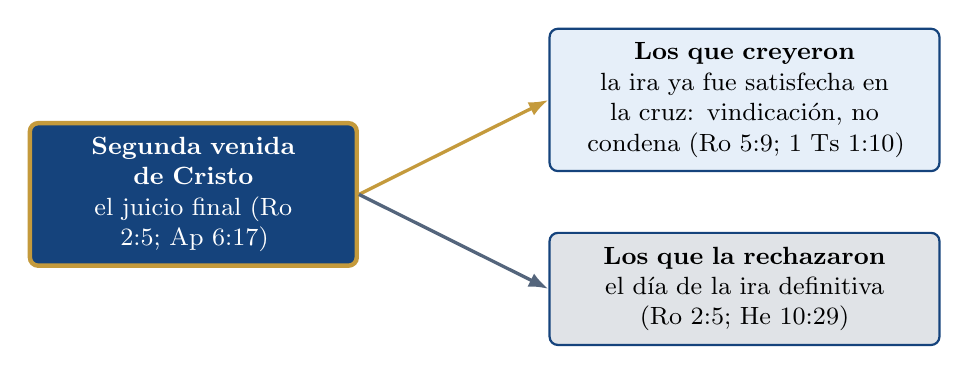
\begin{tikzpicture}[font=\small,
  b/.style={draw=azul,line width=0.8pt,fill=papiro,rounded corners=3pt,text width=4.6cm,align=center,inner sep=5pt}]
 \node[draw=dorado,line width=1.6pt,fill=azul,text=white,rounded corners=3pt,text width=3.8cm,align=center,inner sep=5pt] (v) at (0,0) {\textbf{Segunda venida de Cristo}\\ el juicio final (Ro 2:5; Ap 6:17)};
 \node[b,fill=celeste!15] (c) at (7,1.2) {\textbf{Los que creyeron}\\ la ira ya fue satisfecha en la cruz: vindicación, no condena (Ro 5:9; 1~Ts 1:10)};
 \node[b,fill=gris!18] (r) at (7,-1.2) {\textbf{Los que la rechazaron}\\ el día de la ira definitiva (Ro 2:5; He 10:29)};
 \draw[-{Latex[length=2.5mm]},dorado,line width=1.2pt] (v.east)--(c.west);
 \draw[-{Latex[length=2.5mm]},gris,line width=1.2pt] (v.east)--(r.west);
\end{tikzpicture}\par
{\footnotesize\color{gris}\textit{Figura 6.} El juicio final como Yom Kipur. \textit{Nota.} Elaboración propia.}
\end{center}

\precision{llamar al juicio final ``el Yom Kipur final'' es una lectura tipológica del material de estudio de esta serie; ningún texto bíblico lo nombra así.}

Sofonías, el profeta del ``día de ira'', deja una puerta abierta:

\begin{verso}{Sofonías 2:3}
Buscad a \SENOR{} todos los humildes de la tierra, los que pusisteis por obra su juicio; buscad justicia, buscad mansedumbre; quizás seréis guardados en el día del enojo de \SENOR.
\end{verso}

%===================================================================
\section{Aplicación: vivir ante la ira santa}

La ira de Dios no es una doctrina para asustar ni para esconder. Es una verdad ante la cual se vive. El texto ancla y los demás pasajes sugieren cuatro respuestas:

\begin{enumerate}
\item \textbf{Rendirse a la verdad de Dios.} No suprimirla ni acomodarla a nuestros ídolos. La ira se revela contra los que ``detienen con injusticia la verdad'' (Ro 1:18). ¿Qué verdad sobre Dios estoy deteniendo?
\item \textbf{Arrepentirse y creer hoy.} Hoy es el tiempo de gracia; mañana puede ser demasiado tarde. ``Buscad a \SENOR{}\ldots{} quizás seréis guardados'' (Sof 2:3). La paciencia de Dios es tiempo para arrepentirse, no permiso para seguir (Ro 2:4--5).
\item \textbf{Vivir en gratitud y obediencia.} La humanidad ``no le glorificaron como a Dios, ni le dieron gracias'' (Ro 1:21). El que fue librado de la ira responde con gratitud, y la fe genuina produce obras y honra a Dios.
\item \textbf{Esperar el regreso de Cristo con esperanza y reverencia.} Esperamos ``a Jesús, quien nos libra de la ira venidera'' (1~Ts 1:10). Para el creyente, el gran día final será vindicación, no condena.
\end{enumerate}

Queda una pregunta práctica: ¿qué hacer con nuestra propia ira? Pablo responde con la Torá:

\begin{verso}{Romanos 12:19}
No os venguéis vosotros mismos, amados míos, sino dejad lugar a la ira de Dios; porque escrito está: Mía es la venganza, yo pagaré, dice el Señor.
\end{verso}

\begin{filologiatexto}{Ro 12:19}
Pablo cita Dt 32:35, \heb{לִי נָקָם וְשִׁלֵּם} (\emph{li naqam veshillem}), ``mía es la venganza y la retribución''. Es la raíz \heb{נקם} de Nah 1:2. La venganza es de Dios porque solo él juzga con justicia perfecta; el creyente la deja en sus manos.
\end{filologiatexto}

El creyente puede indignarse ante el mal: ``Airaos, pero no pequéis; no se ponga el sol sobre vuestro enojo'' (Ef 4:26). Pero su ira es vigilada: tiene límite de tiempo y no se convierte en venganza, porque ``la ira del hombre no obra la justicia de Dios'' (Stg 1:20).

%===================================================================
\section{Síntesis}

\begin{tcolorbox}[colback=papiro,colframe=azul,boxrule=1pt,arc=3pt]
La ira de Dios es su respuesta santa, justa y deliberada ante el pecado. ``\SENOR{} es tardo para la ira\ldots{} y no tendrá por inocente al culpable'' (Nah 1:3). Israel la conoció en el Mar Rojo, en el desierto, en Sodoma y en Jerusalén, y también conoció el camino para escapar de ella: el intercesor que se pone entre los muertos y los vivos, y la sangre del Día de la Expiación. Pablo muestra que la ira ``se revela'' junto con la justicia (Ro 1:17--18) y que Dios puso a Cristo como propiciación (Ro 3:25). En la cruz la ira fue satisfecha, la justicia cumplida y el amor derramado; por él ``seremos salvos de la ira'' (Ro 5:9).
\end{tcolorbox}

\begin{center}\small\renewcommand{\arraystretch}{1.3}
\begin{tabular}{@{}L{3.0cm}L{11.4cm}@{}}
\toprule
\textbf{Mirada} & \textbf{Aporte al atributo} \\ \midrule
Hebrea & \emph{af}, \emph{jemá}, \emph{jarón}: la ira que se enciende; \emph{érej appáyim}: lenta para encenderse; la ira como juramento; Aarón entre los muertos y los vivos; \emph{Yom Kippur}. \\
Pink & La ira es perfección divina; es el aborrecimiento eterno del pecado; se ve en la cruz; meditarla produce reverencia y gratitud. \\
Paulina & La ira ``se revela'' junto a la justicia; ``los entregó''; Cristo, el \emph{hilastērion}; el Justo muere por los impíos; salvos de la ira venidera. \\
\bottomrule
\end{tabular}\end{center}

%===================================================================
\section*{Glosario del capítulo}
\begin{description}\setlength{\itemsep}{2pt}
\item[\emph{Af}] (\heb{אַף}). Nariz; por extensión, la ira que se enciende.
\item[\emph{Apotomía}] (\grc{ἀποτομία}). Severidad; literalmente, ``corte tajante'' (Ro 11:22).
\item[\emph{Érej appáyim}] (\heb{אֶרֶךְ אַפַּיִם}). ``Largo de narices'': lento para la ira (Éx 34:6; Nah 1:3).
\item[\emph{Evrá}] (\heb{עֶבְרָה}). Furia que se desborda (Sof 1:15).
\item[\emph{Hilastērion}] (\grc{ἱλαστήριον}). Propiciatorio o propiciación (Ro 3:25); en la LXX, la tapa del arca.
\item[\emph{Jarón}] (\heb{חָרוֹן}). Ardor de la ira.
\item[\emph{Jemá}] (\heb{חֵמָה}). Calor, furor.
\item[\emph{Kapporet}] (\heb{כַּפֹּרֶת}). Tapa del arca del pacto, el propiciatorio.
\item[\emph{Karet}] (\heb{כרת}). Ser ``cortado'' del pueblo (Lv 23:29).
\item[\emph{Kipper}] (\heb{כִּפֶּר}). Expiar, cubrir la culpa.
\item[\emph{Krima}] (\grc{κρίμα}). Juicio, sentencia (1~P 4:17).
\item[\emph{Noqem}] (\heb{נֹקֵם}). Vengador (Nah 1:2).
\item[\emph{Orgē}] (\grc{ὀργή}). Ira; en Pablo, a menudo el juicio final.
\item[\emph{Qétsef}] (\heb{קֶצֶף}). Enojo, indignación (Nm 16:46 [17:11]).
\item[\emph{Thymós}] (\grc{θυμός}). Ardor, furor (Ro 2:8).
\item[\emph{Za'am}] (\heb{זַעַם}). Indignación que denuncia y condena (Nah 1:6).
\end{description}


% ===== Conclusión =====
\backmatter
\chapter*{Referencias}\addcontentsline{toc}{chapter}{Referencias}\markboth{Referencias}{}
\refapa{Bauer, W., Danker, F.~W., Arndt, W.~F., \& Gingrich, F.~W. (2000). \emph{A Greek-English lexicon of the New Testament and other early Christian literature} (3.ª ed.). University of Chicago Press.}
\refapa{Berkhof, L. (1938). \emph{Systematic theology}. Eerdmans.}
\refapa{Berlin, A. (2002). \emph{Lamentations: A commentary}. Westminster John Knox Press.}
\refapa{Block, D.~I. (1999). \emph{Judges, Ruth}. Broadman \& Holman.}
\refapa{Carson, D.~A. (1991). \emph{The Gospel according to John}. Eerdmans.}
\refapa{Charnock, S. (1996). \emph{The existence and attributes of God} (Vols. 1--2). Baker Books. (Obra original publicada en 1682)}
\refapa{Dodd, C.~H. (1935). \emph{The Bible and the Greeks}. Hodder \& Stoughton.}
\refapa{Dunn, J.~D.~G. (1998). \emph{The theology of Paul the apostle}. Eerdmans.}
\refapa{Elbogen, I. (1993). \emph{Jewish liturgy: A comprehensive history} (R.~P. Scheindlin, Trad.). Jewish Publication Society.}
\refapa{Elliger, K., \& Rudolph, W. (Eds.). (1997). \emph{Biblia Hebraica Stuttgartensia} (5.ª ed.). Deutsche Bibelgesellschaft.}
\refapa{Grudem, W. (2007). \emph{Teología sistemática: Una introducción a la doctrina bíblica}. Editorial Vida.}
\refapa{Hays, R.~B. (1989). \emph{Echoes of Scripture in the letters of Paul}. Yale University Press.}
\refapa{Koehler, L., \& Baumgartner, W. (2001). \emph{The Hebrew and Aramaic lexicon of the Old Testament} (M.~E.~J. Richardson, Trad.; Ed. de estudio). Brill.}
\refapa{Marshall, B. J., Armstrong, J. A., McGechie, D. B., \& Glancy, R. J. (1985). Attempt to fulfil Koch's postulates for pyloric \emph{Campylobacter}. \emph{Medical Journal of Australia, 142}(8), 436--439.}
\refapa{Moo, D.~J. (1996). \emph{The epistle to the Romans}. Eerdmans.}
\refapa{Morris, L. (1955). \emph{The apostolic preaching of the cross}. Tyndale Press.}
\refapa{Nestle, E., \& Aland, K. (Eds.). (2012). \emph{Novum Testamentum Graece} (28.ª ed.). Deutsche Bibelgesellschaft.}
\refapa{Oswalt, J.~N. (1986). \emph{The book of Isaiah: Chapters 1--39}. Eerdmans.}
\refapa{Otto, R. (1980). \emph{Lo santo: Lo racional y lo irracional en la idea de Dios} (F. Vela, Trad.). Alianza Editorial. (Obra original publicada en 1917)}
\refapa{Pink, A. W. (2020). \emph{Los atributos de Dios} (E. Rodríguez Cruz, Trad.). Chapel Library. (Obra original publicada en 1930)}
\refapa{Rahlfs, A., \& Hanhart, R. (Eds.). (2006). \emph{Septuaginta} (Ed. rev.). Deutsche Bibelgesellschaft.}
\refapa{Rashi. (s.f.). \emph{Comentario a la Torá} [Gn 1:1; Éx 34:6]. Sefaria. https://www.sefaria.org}
\refapa{Robertson, O.~P. (1990). \emph{The books of Nahum, Habakkuk, and Zephaniah}. Eerdmans.}
\refapa{Sanders, J.~A. (1965). \emph{The Psalms scroll of Qumrân Cave 11 (11QPs\textsuperscript{a})} (Discoveries in the Judaean Desert IV). Clarendon Press.}
\refapa{\emph{Santa Biblia: Reina-Valera 1960}. (1960). Sociedades Bíblicas en América Latina.}
\refapa{Steinsaltz, A. (Ed.). (2017). \emph{Koren Talmud Bavli: Edición William Davidson} [Rosh Hashaná 17b; Shabat 133b; Sotá 14a; Meguilá 31a]. Sefaria. https://www.sefaria.org}
\refapa{Strong, J. (1890). \emph{The exhaustive concordance of the Bible}. Hunt \& Eaton.}
\refapa{\emph{Targum Ónkelos} [Éxodo 34:6--7]. (s.f.). Sefaria. https://www.sefaria.org}
\refapa{Trench, R.~C. (1880). \emph{Synonyms of the New Testament} (9.ª ed.). Macmillan.}
\refapa{Wenham, G.~J. (1987). \emph{Genesis 1--15}. Word.}
\end{document}
